% Options for packages loaded elsewhere
\PassOptionsToPackage{unicode}{hyperref}
\PassOptionsToPackage{hyphens}{url}
\PassOptionsToPackage{dvipsnames,svgnames,x11names}{xcolor}
%
\documentclass[
  letterpaper,
  DIV=11,
  numbers=noendperiod]{scrartcl}

\usepackage{amsmath,amssymb}
\usepackage{setspace}
\usepackage{iftex}
\ifPDFTeX
  \usepackage[T1]{fontenc}
  \usepackage[utf8]{inputenc}
  \usepackage{textcomp} % provide euro and other symbols
\else % if luatex or xetex
  \usepackage{unicode-math}
  \defaultfontfeatures{Scale=MatchLowercase}
  \defaultfontfeatures[\rmfamily]{Ligatures=TeX,Scale=1}
\fi
\usepackage{lmodern}
\ifPDFTeX\else  
    % xetex/luatex font selection
\fi
% Use upquote if available, for straight quotes in verbatim environments
\IfFileExists{upquote.sty}{\usepackage{upquote}}{}
\IfFileExists{microtype.sty}{% use microtype if available
  \usepackage[]{microtype}
  \UseMicrotypeSet[protrusion]{basicmath} % disable protrusion for tt fonts
}{}
\makeatletter
\@ifundefined{KOMAClassName}{% if non-KOMA class
  \IfFileExists{parskip.sty}{%
    \usepackage{parskip}
  }{% else
    \setlength{\parindent}{0pt}
    \setlength{\parskip}{6pt plus 2pt minus 1pt}}
}{% if KOMA class
  \KOMAoptions{parskip=half}}
\makeatother
\usepackage{xcolor}
\setlength{\emergencystretch}{3em} % prevent overfull lines
\setcounter{secnumdepth}{-\maxdimen} % remove section numbering
% Make \paragraph and \subparagraph free-standing
\makeatletter
\ifx\paragraph\undefined\else
  \let\oldparagraph\paragraph
  \renewcommand{\paragraph}{
    \@ifstar
      \xxxParagraphStar
      \xxxParagraphNoStar
  }
  \newcommand{\xxxParagraphStar}[1]{\oldparagraph*{#1}\mbox{}}
  \newcommand{\xxxParagraphNoStar}[1]{\oldparagraph{#1}\mbox{}}
\fi
\ifx\subparagraph\undefined\else
  \let\oldsubparagraph\subparagraph
  \renewcommand{\subparagraph}{
    \@ifstar
      \xxxSubParagraphStar
      \xxxSubParagraphNoStar
  }
  \newcommand{\xxxSubParagraphStar}[1]{\oldsubparagraph*{#1}\mbox{}}
  \newcommand{\xxxSubParagraphNoStar}[1]{\oldsubparagraph{#1}\mbox{}}
\fi
\makeatother


\providecommand{\tightlist}{%
  \setlength{\itemsep}{0pt}\setlength{\parskip}{0pt}}\usepackage{longtable,booktabs,array}
\usepackage{calc} % for calculating minipage widths
% Correct order of tables after \paragraph or \subparagraph
\usepackage{etoolbox}
\makeatletter
\patchcmd\longtable{\par}{\if@noskipsec\mbox{}\fi\par}{}{}
\makeatother
% Allow footnotes in longtable head/foot
\IfFileExists{footnotehyper.sty}{\usepackage{footnotehyper}}{\usepackage{footnote}}
\makesavenoteenv{longtable}
\usepackage{graphicx}
\makeatletter
\newsavebox\pandoc@box
\newcommand*\pandocbounded[1]{% scales image to fit in text height/width
  \sbox\pandoc@box{#1}%
  \Gscale@div\@tempa{\textheight}{\dimexpr\ht\pandoc@box+\dp\pandoc@box\relax}%
  \Gscale@div\@tempb{\linewidth}{\wd\pandoc@box}%
  \ifdim\@tempb\p@<\@tempa\p@\let\@tempa\@tempb\fi% select the smaller of both
  \ifdim\@tempa\p@<\p@\scalebox{\@tempa}{\usebox\pandoc@box}%
  \else\usebox{\pandoc@box}%
  \fi%
}
% Set default figure placement to htbp
% \makeatother
% definitions for citeproc citations
\NewDocumentCommand\citeproctext{}{}
\NewDocumentCommand\citeproc{mm}{%
  \begingroup\def\citeproctext{#2}\cite{#1}\endgroup}
\makeatletter
 % allow citations to break across lines
 \let\@cite@ofmt\@firstofone
 % avoid brackets around text for \cite:
 \def\@biblabel#1{}
 \def\@cite#1#2{{#1\if@tempswa , #2\fi}}
\makeatother
\newlength{\cslhangindent}
\setlength{\cslhangindent}{1.5em}
\newlength{\csllabelwidth}
\setlength{\csllabelwidth}{3em}
\newenvironment{CSLReferences}[2] % #1 hanging-indent, #2 entry-spacing
 {\begin{list}{}{%
  \setlength{\itemindent}{0pt}
  \setlength{\leftmargin}{0pt}
  \setlength{\parsep}{0pt}
  % turn on hanging indent if param 1 is 1
  \ifodd #1
   \setlength{\leftmargin}{\cslhangindent}
   \setlength{\itemindent}{-1\cslhangindent}
  \fi
  % set entry spacing
  \setlength{\itemsep}{#2\baselineskip}}}
 {\end{list}}
\usepackage{calc}
\newcommand{\CSLBlock}[1]{\hfill\break\parbox[t]{\linewidth}{\strut\ignorespaces#1\strut}}
\newcommand{\CSLLeftMargin}[1]{\parbox[t]{\csllabelwidth}{\strut#1\strut}}
\newcommand{\CSLRightInline}[1]{\parbox[t]{\linewidth - \csllabelwidth}{\strut#1\strut}}
\newcommand{\CSLIndent}[1]{\hspace{\cslhangindent}#1}

\usepackage{fontspec}
\usepackage{multirow}
\usepackage{multicol}
\usepackage{colortbl}
\usepackage{ulem}
\usepackage{hhline}
\newlength\Oldarrayrulewidth
\newlength\Oldtabcolsep
\usepackage{longtable}
\usepackage{array}
\usepackage{hyperref}
\usepackage{float}
\usepackage{wrapfig}
\KOMAoption{captions}{tableheading}
\makeatletter
\@ifpackageloaded{caption}{}{\usepackage{caption}}
\AtBeginDocument{%
\ifdefined\contentsname
  \renewcommand*\contentsname{Table of contents}
\else
  \newcommand\contentsname{Table of contents}
\fi
\ifdefined\listfigurename
  \renewcommand*\listfigurename{List of Figures}
\else
  \newcommand\listfigurename{List of Figures}
\fi
\ifdefined\listtablename
  \renewcommand*\listtablename{List of Tables}
\else
  \newcommand\listtablename{List of Tables}
\fi
\ifdefined\figurename
  \renewcommand*\figurename{Figure}
\else
  \newcommand\figurename{Figure}
\fi
\ifdefined\tablename
  \renewcommand*\tablename{Table}
\else
  \newcommand\tablename{Table}
\fi
}
\@ifpackageloaded{float}{}{\usepackage{float}}
\floatstyle{ruled}
\@ifundefined{c@chapter}{\newfloat{codelisting}{h}{lop}}{\newfloat{codelisting}{h}{lop}[chapter]}
\floatname{codelisting}{Listing}
\newcommand*\listoflistings{\listof{codelisting}{List of Listings}}
\makeatother
\makeatletter
\makeatother
\makeatletter
\@ifpackageloaded{caption}{}{\usepackage{caption}}
\@ifpackageloaded{subcaption}{}{\usepackage{subcaption}}
\makeatother

\usepackage{bookmark}

\IfFileExists{xurl.sty}{\usepackage{xurl}}{} % add URL line breaks if available
\urlstyle{same} % disable monospaced font for URLs
\hypersetup{
  pdftitle={Hiding in the trees: Unmasking a cryptic genus of arboreal New Guinea frogs with phylogenetic taxonomy},
  pdfauthor={Allison R Fisher, Ke Cao, Allen Allison, Bulisa Iova, and Marguerite A Butler},
  pdfkeywords={frogs, homoplasy, indo-pacific, morphology, new
classification, new genera, phylogenetic nomenclature, phylogenetics},
  colorlinks=true,
  linkcolor={blue},
  filecolor={Maroon},
  citecolor={Blue},
  urlcolor={Blue},
  pdfcreator={LaTeX via pandoc}}


\title{Hiding in the trees: Unmasking a cryptic genus of arboreal New
Guinea frogs with phylogenetic taxonomy}
\author{Allison R Fisher, Ke Cao, Allen Allison, Bulisa Iova, and
Marguerite A Butler}
\date{2026-06-15}

\begin{document}
\maketitle


\setstretch{2}
\newpage{}

\section{Abstract}\label{abstract}

Although cryptic species are known to underestimate biodiversity,
cryptic genera may present greater challenges for evolutionary studies.
Surprisingly there remain long-standing groups that contain unrecognized
polyphyly because they are morphologically undiagnosable. As new species
are described, even when molecular phylogenetic analysis is included,
the only way to identify cryptic polyphyly is via the inclusion of
appropriate outgroups -- however, there are no clues that there are any
problem with monophyly. Absent appropriate outgroups, the resulting
phylogenies may falsely appear to contain a single monophyletic group,
leading to the growth of cryptic polyphyletic groups. One example is the
frog genus \emph{Oreophryne}, recently discovered as polyphyletic
despite 130 years of research. Here we show that the two clades are
morphologically undiagnosible and define the clades using phylogenetic
taxonomy. We include the type species \emph{O. senckenbergiana},
resolving which clade retains the name \emph{Oreophryne}, and name the
strikingly similar genus of arboreal frogs \textbf{\emph{Auparoparo}
gen. nov.} from the indigenous Papuan language Motu. Their geographic
distributions implicate plate tectonic activity in diversification, with
\emph{Oreophryne} distributed from the Philippines to Indonesia, along
central to south New Guinea and its satellite islands, whereas
\emph{Auparoparo} occurs in Sulawesi and southern New Guinea and
satellite islands where there is range overlap. We caution that groups
with unrecognized polyphyly are still in use today, renewing a call for
careful confirmation of monophyly to promote nomenclatural stability and
improve the accuracy of evolutionary conclusions.

\newpage{}

\section{Introduction}\label{introduction}

\emph{Oreophryne} (Boettger, 1895) is the oldest and arguably the best
studied genus of the hyperdivsere subfamily Asterophryinae. Well known
for its aboreal morphology and lifestyle, the taxonomy of the genus
\emph{Oreophryne} as currently recognized has been stable over the past
century, until it was recently discovered that the single large clade
is, in fact, two independently evolved clades (reviewed in Hill \emph{et
al.}, 2022). A natural question is how did this happen and why did it
remain undiscovered for so long? One obvious answer is that their
morphology is remarkably similar (Figure~\ref{fig-photos}).
\emph{Oreophryne} are consipicuously arboreal and account for nearly all
arboreal species of Asterophryinae (Günther, Richards, \& Iskandar,
2001; Menzies, 2006), inhabiting lowland to montane rain forest,
although there is a small group of diminutive, high-elevation, grassland
species, a few of which are terrestrial (Zweifel, Cogger, \& Richards,
2005; Günther \& Richards, 2012; Putri \emph{et al.}, 2023). In short,
\emph{Oreophryne} are morphologically distinctive, consistent with their
arboreal lifestyle, and appear in the field to be a natural group
preserved by niche conservatism.

Although the taxonomic instability is well known in the history of the
subfamily Asterophyinae (reviewed in Rivera \emph{et al.}, 2017; Hill
\emph{et al.}, 2022), it appeared that \emph{Oreophryne} was united by a
useful diagnostic character distinct from all other genera. Based on a
pectoral anatomy with highly reduced and distinctly curved clavicles
(Parker, 1934; Zweifel, 2003), hypothetical new species could be
assigned to \emph{Oreophryne}, and for modern studies, confirmed by
phylogenetic analysis with other members of \emph{Oreophryne}. Over the
past 130 years the genus \emph{Oreophryne} has grown to 75 currently
recognized species, fully 1/5 of the total diversity of subfamily
Asterophryinae and the largest of the \textasciitilde16 genera (Hill
\emph{et al.}, 2022; Frost, 2024). \emph{Oreophryne} as currently
recognized has the largest geographic distribution in the subfamily
(Hill \emph{et al.}, 2023a), with species centered on mainland New
Guinea and its offshore islands (Werner, 1898; Zweifel, 1956; Zweifel,
Menzies, \& Price, 2003; Kraus \& Allison, 2004; Kraus \& Allison, 2009;
Kraus, 2013; Frost, 2024), but ranging westward to distant oceanic
islands (Müller, 1894; Boulenger, 1896; Ahl, 1933; Putri \emph{et al.},
2023) and northward to Indonesia (Boettger, 1895; Setiadi \emph{et al.},
2010; Günther, Iskandar, \& Richards, 2023) and the Southern Philippines
Islands (Alcala, 1986; Balinton \& Seña, 2015).

The apparently reliable diagnostic character, however, has never been
demonstrated to be a synapomorphy, and recent studies have not found
evidence for monophyly (Zweifel \emph{et al.}, 2005; Rivera \emph{et
al.}, 2017). Recently, Hill et. al (2022, 2023b) established that
\emph{Oreophryne} sensu lato represents two reciprocally monophyletic
groups that are not sister taxa (Figure~\ref{fig-phylo}), temporarily
labeled ``\emph{Oreophryne} A'' and ``\emph{Oreophryne} B''.
Furthermore, it is unknown whether it is possible to identify these
groups with any morphological characters -- there may in fact be no
reliable diagnostic characters, rendering phylogenetic taxonomic
definitions for each clade an imperative for evolutionary study. The
aims of this study are to assess the phylogenetic position of the newly
available type species of \emph{Oreophryne} (\emph{Oreophryne
senkenbergiana}) to name and describe the new genus, and to develop
phylogenetic definitions for both clades in the context of the
subfamily-level Asterophrinae phylogeny including representatives from
all known genera. Furthermore, we analyze the morphological
characteristics to assess whether morphological diagnosis is possible,
and consider whether there are any additional features to assist
collectors when identifying putative \emph{Oreophryne} in the field
(e.g., call type, geography, other characters), and discuss the
implications of having misleading diagnostic characters for evolutionary
studies. Inclusion of samples in molecular phylogenetics is not enough,
and indeed it is necessary to include explicit tests of monophyly when
proposing a new taxonomy.

\paragraph{Taxonomic History:}\label{taxonomic-history}

Boettger (1895) described the genus \emph{Oreoprhyne} and the species
\emph{Oreophryne senckenbergiana} on the basis of two specimens from
Halmahera Island, in the Maluku Archipelago west of New Guinea, that
lacked procoracoids and had cartilaginous sterna. He also noted the
presence of expanded finger pads and transverse folds of skin in the
palate. Parker (1934) noted that procoracoids were present, but were
reduced and re-diagnosed the genus on the basis of this feature together
with the presence of reduced clavicles, no omosternum, and a large
cartilaginous sternum. Zweifel (2003) noted that ``the clavicles are
tiny, slightly curved bones lying on (ventral to) the procoracoid
cartilage and apart from the midline and the scapula.'' On the basis of
these features there are now 75 recognized species in the genus (Frost,
2024).

\begin{figure}

\centering{

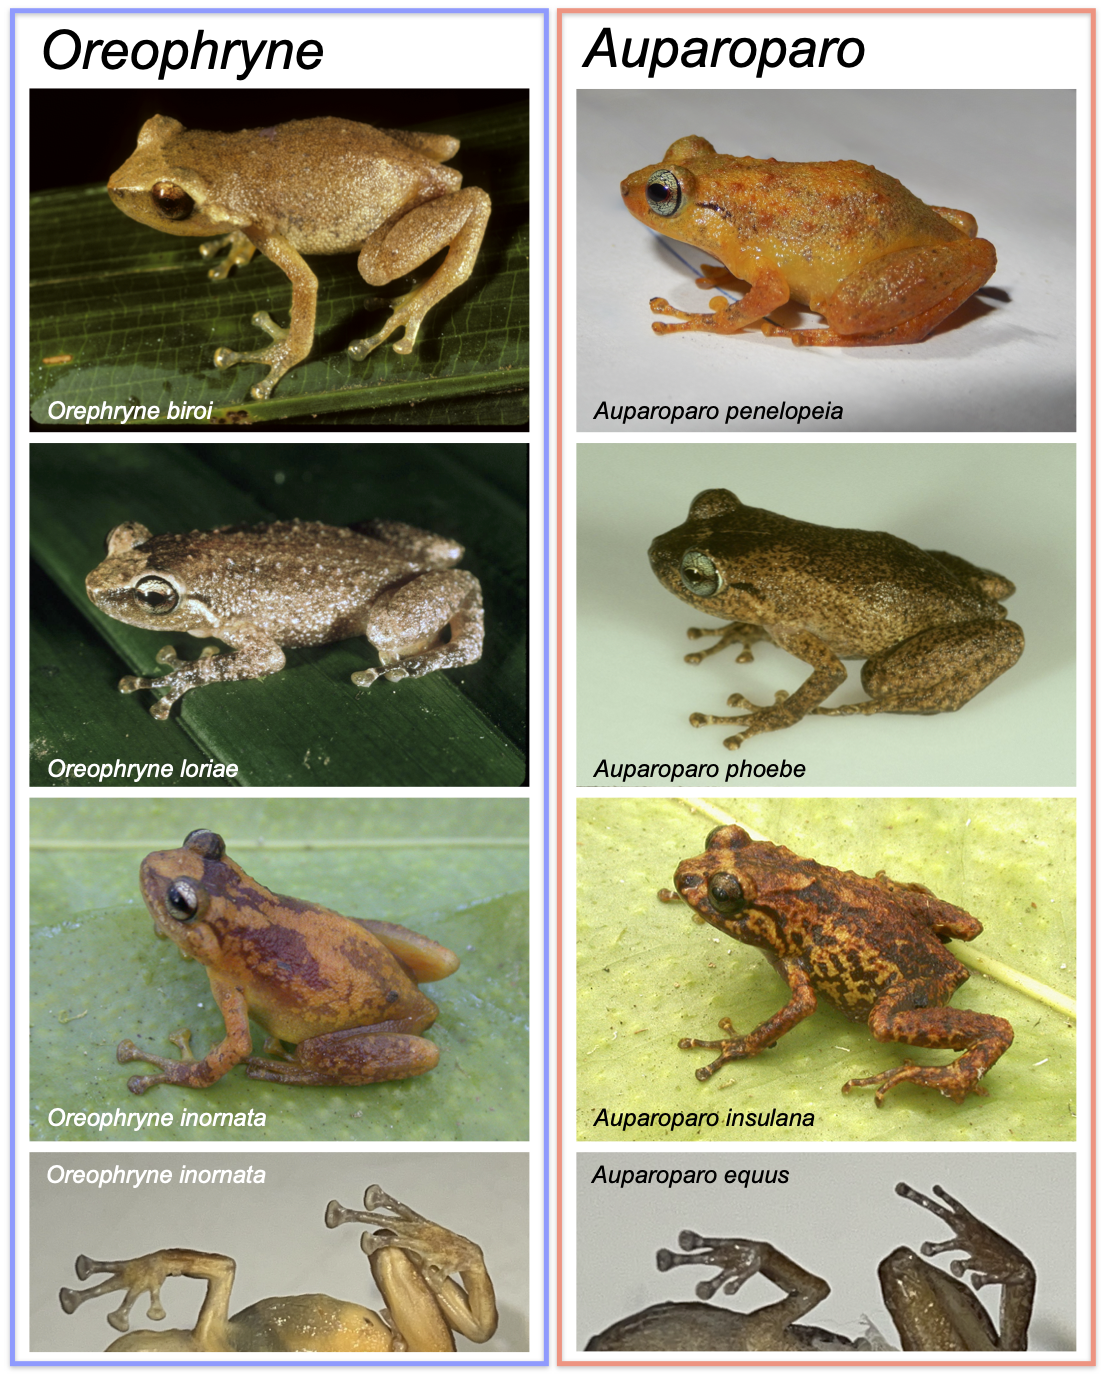
\includegraphics[width=0.8\linewidth,height=\textheight,keepaspectratio]{../Results/fig1.frogs.png}

}

\caption{\label{fig-photos}Photos of \emph{Oreophryne} species on the
left, \emph{Auparoparo} species on the right. Both genera are aboreal
with a few exceptions as noted in the text, and contain nearly all
arboreal species within Asterophryinae. Comparison of finger and toe pad
sizes in \emph{Oreophryne inornata} BPBM16217 vs.~\emph{Auparoparo
equus} BPBM15775, bottom row.}

\end{figure}%

While \emph{Oreophryne} sensu lato is morphologically similar
(Figure~\ref{fig-photos}), large scale molecular phylogenetic analysis
with many ingroup samples were required to clarify that this group
contains two reciprocally monophyletic clades that are not sister taxa
(Hill \emph{et al.}, 2022, 2023b). Early molecular phylogenetic studies
suggested monophyly but only included a few taxa within a larger-scale
study (Köhler \& Günther, 2008 included 9 \emph{Oreophryne} species; De
Sa \emph{et al.}, 2012 included 4). Rivera \emph{et al.} (2017) provided
the first molecular evidence of a polyphyletic \emph{Oreophryne} with 36
\emph{Oreophryne} species within a larger phylogeny Asterophryinae which
included 155 samples, followed by Tu \emph{et al.} (2018)'s sparse
supermatrix approach with 18 species of \emph{Oreophryne} falling out in
various places within a much larger phylogeny, but both of these lacked
strong nodal support connecting the hypothesized clades to the backbone
of the phylogeny. The polyphyletic nature of \emph{Oreophryne} sensu
lato was not clearly demonstrated until Hill et. al (2022, 2023b)
included 44 species of \emph{Oreophryne} (with data 96\% complete for
sampled loci) within a 218 taxon phylogeny of Asterophryinae. This
phylogeny is the most complete and robust phylogeny to date. The two
clades, labeled ``\emph{Oreophryne} A'' and ``\emph{Oreophryne} B'' have
deep histories of \textasciitilde{} 18MY and \textasciitilde16MY,
respectively, with ``\emph{Oreophryne} A'' sister to the rest of the
subfamily (2022, 2023b).

\section{Materials and Methods}\label{materials-and-methods}

\subsection{Taxon Sampling}\label{taxon-sampling}

Asterophryinae is an adaptive radiation with short branch lengths along
the backbone separating currently recognized genera (Rivera \emph{et
al.}, 2017; Hill \emph{et al.}, 2022, 2023b); we reconstruct the
phylogeny of \emph{Oreophryne} sensu lato within the larger context of
the subfamily. We include 30 named species and 18 unnamed species of
\emph{Oreophryne} within a larger dataset of 234 samples of 203 species
of Asterophryinae collected across New Guinea, the Philippines, and
Indonesia with three outgroup species to root the phylogeny
(\emph{Dyscophus antongilii}, \emph{Scaphiophryne marmorata}, and
\emph{Platypelis grandis}). Importantly, we include the type species
\emph{Oreophryne senckenbergiana} (Boettger, 1895) in a molecular
phylogeny for the first time. The samples were collected in Halmahera,
North Maluku Province, Indonesia by Iqbal Setiadi
, Table~\ref{tbl-localities}, near the type locality for \emph{O.
senkenbergiana} (Halmahera, Indonesia as documented by Boettger, 1895).

\global\setlength{\Oldarrayrulewidth}{\arrayrulewidth}

\global\setlength{\Oldtabcolsep}{\tabcolsep}

\setlength{\tabcolsep}{2pt}

\renewcommand*{\arraystretch}{1.5}



\providecommand{\ascline}[3]{\noalign{\global\arrayrulewidth #1}\arrayrulecolor[HTML]{#2}\cline{#3}}

\begin{longtable}[c]{|p{0.88in}|p{2.19in}|p{2.36in}|p{1.36in}}

\caption{\label{tbl-localities}Locality information for samples
sequenced in this study. See Hill, et al., 2023, Table 1 for additional
metadata.}

\tabularnewline

\ascline{1.5pt}{666666}{1-4}

\multicolumn{1}{>{\raggedright}b{\dimexpr 0.88in+0\tabcolsep}}{} & \multicolumn{1}{>{\raggedright}b{\dimexpr 2.19in+0\tabcolsep}}{} & \multicolumn{1}{>{\raggedright}b{\dimexpr 2.36in+0\tabcolsep}}{} & \multicolumn{1}{>{\raggedright}m{\dimexpr 1.36in+0\tabcolsep}}{\advance\leftskip by 2.0pt\relax \advance\rightskip by 2.0pt\relax \textcolor[HTML]{666666}{\fontsize{11}{11}\selectfont{{\fontspec{Helvetica} Latitude}}}} \\





\multicolumn{1}{>{\raggedright}b{\dimexpr 0.88in+0\tabcolsep}}{\advance\leftskip by 2.0pt\relax \advance\rightskip by 2.0pt\relax \textcolor[HTML]{666666}{\fontsize{11}{11}\selectfont{{\fontspec{Helvetica} ID}}}} & \multicolumn{1}{>{\raggedright}b{\dimexpr 2.19in+0\tabcolsep}}{\advance\leftskip by 2.0pt\relax \advance\rightskip by 2.0pt\relax \textcolor[HTML]{666666}{\fontsize{11}{11}\selectfont{{\fontspec{Helvetica} Species}}}} & \multicolumn{1}{>{\raggedright}b{\dimexpr 2.36in+0\tabcolsep}}{\advance\leftskip by 2.0pt\relax \advance\rightskip by 2.0pt\relax \textcolor[HTML]{666666}{\fontsize{11}{11}\selectfont{{\fontspec{Helvetica} Locality}}}} & \multicolumn{1}{>{\raggedright}m{\dimexpr 1.36in+0\tabcolsep}}{\advance\leftskip by 2.0pt\relax \advance\rightskip by 2.0pt\relax \textcolor[HTML]{666666}{\fontsize{11}{11}\selectfont{{\fontspec{Helvetica} Latitude,\ Longitude}}}} \\

\ascline{1.5pt}{666666}{1-4}\endfirsthead 

\ascline{1.5pt}{666666}{1-4}

\multicolumn{1}{>{\raggedright}b{\dimexpr 0.88in+0\tabcolsep}}{} & \multicolumn{1}{>{\raggedright}b{\dimexpr 2.19in+0\tabcolsep}}{} & \multicolumn{1}{>{\raggedright}b{\dimexpr 2.36in+0\tabcolsep}}{} & \multicolumn{1}{>{\raggedright}m{\dimexpr 1.36in+0\tabcolsep}}{\advance\leftskip by 2.0pt\relax \advance\rightskip by 2.0pt\relax \textcolor[HTML]{666666}{\fontsize{11}{11}\selectfont{{\fontspec{Helvetica} Latitude}}}} \\





\multicolumn{1}{>{\raggedright}b{\dimexpr 0.88in+0\tabcolsep}}{\advance\leftskip by 2.0pt\relax \advance\rightskip by 2.0pt\relax \textcolor[HTML]{666666}{\fontsize{11}{11}\selectfont{{\fontspec{Helvetica} ID}}}} & \multicolumn{1}{>{\raggedright}b{\dimexpr 2.19in+0\tabcolsep}}{\advance\leftskip by 2.0pt\relax \advance\rightskip by 2.0pt\relax \textcolor[HTML]{666666}{\fontsize{11}{11}\selectfont{{\fontspec{Helvetica} Species}}}} & \multicolumn{1}{>{\raggedright}b{\dimexpr 2.36in+0\tabcolsep}}{\advance\leftskip by 2.0pt\relax \advance\rightskip by 2.0pt\relax \textcolor[HTML]{666666}{\fontsize{11}{11}\selectfont{{\fontspec{Helvetica} Locality}}}} & \multicolumn{1}{>{\raggedright}m{\dimexpr 1.36in+0\tabcolsep}}{\advance\leftskip by 2.0pt\relax \advance\rightskip by 2.0pt\relax \textcolor[HTML]{666666}{\fontsize{11}{11}\selectfont{{\fontspec{Helvetica} Latitude,\ Longitude}}}} \\

\ascline{1.5pt}{666666}{1-4}\endhead



\multicolumn{1}{>{\raggedright}m{\dimexpr 0.88in+0\tabcolsep}}{\advance\leftskip by 2.0pt\relax \advance\rightskip by 2.0pt\relax \textcolor[HTML]{666666}{\fontsize{11}{11}\selectfont{{\fontspec{Helvetica} BJE01143}}}} & \multicolumn{1}{>{\raggedright}m{\dimexpr 2.19in+0\tabcolsep}}{\advance\leftskip by 2.0pt\relax \advance\rightskip by 2.0pt\relax \textcolor[HTML]{666666}{\fontsize{11}{11}\selectfont{{\fontspec{Helvetica} \textit{Oreophryne\ senckenbergiana}}}}} & \multicolumn{1}{>{\raggedright}m{\dimexpr 2.36in+0\tabcolsep}}{\advance\leftskip by 2.0pt\relax \advance\rightskip by 2.0pt\relax \textcolor[HTML]{666666}{\fontsize{11}{11}\selectfont{{\fontspec{Helvetica} Kabupaten\ Halmahera\ Utara,}}}\textcolor[HTML]{666666}{\fontsize{11}{11}\selectfont{{\fontspec{Helvetica} \linebreak }}}\textcolor[HTML]{666666}{\fontsize{11}{11}\selectfont{{\fontspec{Helvetica} Halmahera\ Island,\ North\ Maluku}}}} & \multicolumn{1}{>{\raggedright}m{\dimexpr 1.36in+0\tabcolsep}}{\advance\leftskip by 2.0pt\relax \advance\rightskip by 2.0pt\relax \textcolor[HTML]{666666}{\fontsize{11}{11}\selectfont{{\fontspec{Helvetica} 1.7899,\ 127.8910}}}} \\





\multicolumn{1}{>{\raggedright}m{\dimexpr 0.88in+0\tabcolsep}}{\advance\leftskip by 2.0pt\relax \advance\rightskip by 2.0pt\relax \textcolor[HTML]{666666}{\fontsize{11}{11}\selectfont{{\fontspec{Helvetica} BJE01144}}}} & \multicolumn{1}{>{\raggedright}m{\dimexpr 2.19in+0\tabcolsep}}{\advance\leftskip by 2.0pt\relax \advance\rightskip by 2.0pt\relax \textcolor[HTML]{666666}{\fontsize{11}{11}\selectfont{{\fontspec{Helvetica} \textit{Oreophryne\ senckenbergiana}}}}} & \multicolumn{1}{>{\raggedright}m{\dimexpr 2.36in+0\tabcolsep}}{\advance\leftskip by 2.0pt\relax \advance\rightskip by 2.0pt\relax \textcolor[HTML]{666666}{\fontsize{11}{11}\selectfont{{\fontspec{Helvetica} Kabupaten\ Halmahera\ Utara,}}}\textcolor[HTML]{666666}{\fontsize{11}{11}\selectfont{{\fontspec{Helvetica} \linebreak }}}\textcolor[HTML]{666666}{\fontsize{11}{11}\selectfont{{\fontspec{Helvetica} Halmahera\ Island,\ North\ Maluku}}}} & \multicolumn{1}{>{\raggedright}m{\dimexpr 1.36in+0\tabcolsep}}{\advance\leftskip by 2.0pt\relax \advance\rightskip by 2.0pt\relax \textcolor[HTML]{666666}{\fontsize{11}{11}\selectfont{{\fontspec{Helvetica} 1.7899,\ 127.8910}}}} \\





\multicolumn{1}{>{\raggedright}m{\dimexpr 0.88in+0\tabcolsep}}{\advance\leftskip by 2.0pt\relax \advance\rightskip by 2.0pt\relax \textcolor[HTML]{666666}{\fontsize{11}{11}\selectfont{{\fontspec{Helvetica} BJE01120}}}} & \multicolumn{1}{>{\raggedright}m{\dimexpr 2.19in+0\tabcolsep}}{\advance\leftskip by 2.0pt\relax \advance\rightskip by 2.0pt\relax \textcolor[HTML]{666666}{\fontsize{11}{11}\selectfont{{\fontspec{Helvetica} \textit{Oreophryne\ senckenbergiana}}}}} & \multicolumn{1}{>{\raggedright}m{\dimexpr 2.36in+0\tabcolsep}}{\advance\leftskip by 2.0pt\relax \advance\rightskip by 2.0pt\relax \textcolor[HTML]{666666}{\fontsize{11}{11}\selectfont{{\fontspec{Helvetica} Kabupaten\ Halmahera\ Utara,}}}\textcolor[HTML]{666666}{\fontsize{11}{11}\selectfont{{\fontspec{Helvetica} \linebreak }}}\textcolor[HTML]{666666}{\fontsize{11}{11}\selectfont{{\fontspec{Helvetica} Halmahera\ Island,\ North\ Maluku}}}} & \multicolumn{1}{>{\raggedright}m{\dimexpr 1.36in+0\tabcolsep}}{\advance\leftskip by 2.0pt\relax \advance\rightskip by 2.0pt\relax \textcolor[HTML]{666666}{\fontsize{11}{11}\selectfont{{\fontspec{Helvetica} 1.8228,\ 127.8300}}}} \\

\ascline{1.5pt}{666666}{1-4}


\end{longtable}

\arrayrulecolor[HTML]{000000}

\global\setlength{\arrayrulewidth}{\Oldarrayrulewidth}

\global\setlength{\tabcolsep}{\Oldtabcolsep}

\renewcommand*{\arraystretch}{1}

\subsubsection{Molecular Sequence}\label{molecular-sequence}

We obtained nearly complete DNA sequence data for five loci (three
nuclear: Seventh in Absentia {[}SIA{]}, Brain Derived Neurotrophic
Factor {[}BDNF{]}, Sodium Calcium Exchange subunit-1 {[}NXC-1{]}, and
two mitochondrial loci (Cytochrome oxidase b {[}CYTB{]}, and NADH
dehydrogenase subunit 4 {[}ND4{]} from four samples of two species not
previously sequenced and combined these with previously published data
(Rivera \emph{et al.}, 2017; Hill \emph{et al.}, 2022, 2023b) for a
dataset of 240 samples with 207 species and 2475 base pairs that is 96\%
complete. All loci were complete for the added samples. Sequence quality
was evaluated using chromatogram quality scores, checks for stop codons
indicating pseudogenes, BLAST searches (Ye \emph{et al.}, 2012), and
concordance of pairwise similarities with other Asterophryinae
sequences. Primer sequences and detailed methods are provided in (Hill
\emph{et al.}, 2023b). We note that we excluded from the previous
alignment (Hill \emph{et al.}, 2022, 2023b) two samples of
\emph{Aphantophryne pansa} (BPBM 5299 and BPBM 8312) which were deemed
unreliable as they came from formalin-fixed material, and three samples
which fell out in odd places that should be confirmed with new material
prior to recommending taxonomic revision (BPBM 22708 \emph{Copiula
tyleri}, BPBM 38939 \emph{Copiula sp. 7}, BPBM 37753 \emph{Paedophryne
dekot}). We note that genetic material from 47 species of
\emph{Oreophryne} sensu lato was not available for this molecular
analysis.

\subsubsection{Morphology, Behavior, and Geographic
Distribution}\label{morphology-behavior-and-geographic-distribution}

We collected new morphological characters and reexamined traits compiled
from the literature , character states defined in
Table~\ref{tbl-morphcharacters} for all named species of
\emph{Oreophryne} in our phylogenetic dataset. Our sample included all
species available in the collections of the Bishop Museum, Honolulu,
Hawaii (BPBM): thirteen species of ``\emph{Oreophryne} A'', eight
species ``\emph{Oreophryne} B'' (Table~\ref{tbl-morph}). Finger and toe
pads were photographed and length and width of the toe tips were
measured using ImageJ software. Trait information for the remaining
species were gathered from the literature, six species of
\_``Oreophryne\_ A'' and one of ``\emph{Oreophryne} B''. In addition, we
compiled information on call type from the literature and collection
location from the respective collectors or the BPBM database (global
positioning coordinates {[}GPS{]}; Table~\ref{tbl-morph}). We examined
the ability of morphological and behavioral characters to provide a
diagnosis to the two \emph{Oreophryne} clades consistent with molecular
phylogenetics.

\global\setlength{\Oldarrayrulewidth}{\arrayrulewidth}

\global\setlength{\Oldtabcolsep}{\tabcolsep}

\setlength{\tabcolsep}{2pt}

\renewcommand*{\arraystretch}{1.5}



\providecommand{\ascline}[3]{\noalign{\global\arrayrulewidth #1}\arrayrulecolor[HTML]{#2}\cline{#3}}

\begin{longtable}[c]{|p{0.70in}|p{1.86in}|p{5.32in}}

\caption{\label{tbl-morphcharacters}Description of traits surveyed.}

\tabularnewline

\ascline{1.5pt}{666666}{1-3}

\multicolumn{1}{>{\raggedright}m{\dimexpr 0.7in+0\tabcolsep}}{\advance\leftskip by 2.0pt\relax \advance\rightskip by 2.0pt\relax \textcolor[HTML]{666666}{\fontsize{11}{11}\selectfont{{\fontspec{Helvetica} Column*}}}} & \multicolumn{1}{>{\raggedright}m{\dimexpr 1.86in+0\tabcolsep}}{\advance\leftskip by 2.0pt\relax \advance\rightskip by 2.0pt\relax \textcolor[HTML]{666666}{\fontsize{11}{11}\selectfont{{\fontspec{Helvetica} Trait}}}} & \multicolumn{1}{>{\raggedright}m{\dimexpr 5.32in+0\tabcolsep}}{\advance\leftskip by 2.0pt\relax \advance\rightskip by 2.0pt\relax \textcolor[HTML]{666666}{\fontsize{11}{11}\selectfont{{\fontspec{Helvetica} Definition}}}} \\

\ascline{1.5pt}{666666}{1-3}\endfirsthead 

\ascline{1.5pt}{666666}{1-3}

\multicolumn{1}{>{\raggedright}m{\dimexpr 0.7in+0\tabcolsep}}{\advance\leftskip by 2.0pt\relax \advance\rightskip by 2.0pt\relax \textcolor[HTML]{666666}{\fontsize{11}{11}\selectfont{{\fontspec{Helvetica} Column*}}}} & \multicolumn{1}{>{\raggedright}m{\dimexpr 1.86in+0\tabcolsep}}{\advance\leftskip by 2.0pt\relax \advance\rightskip by 2.0pt\relax \textcolor[HTML]{666666}{\fontsize{11}{11}\selectfont{{\fontspec{Helvetica} Trait}}}} & \multicolumn{1}{>{\raggedright}m{\dimexpr 5.32in+0\tabcolsep}}{\advance\leftskip by 2.0pt\relax \advance\rightskip by 2.0pt\relax \textcolor[HTML]{666666}{\fontsize{11}{11}\selectfont{{\fontspec{Helvetica} Definition}}}} \\

\ascline{1.5pt}{666666}{1-3}\endhead



\multicolumn{3}{>{\raggedright}m{\dimexpr 7.88in+4\tabcolsep}}{\advance\leftskip by 2.0pt\relax \advance\rightskip by 2.0pt\relax \textcolor[HTML]{666666}{\fontsize{11}{11}\selectfont{{\fontspec{Helvetica} *Corresponding\ column\ in\ Table\ 3.\ The\ last\ three\ traits\ were\ scored\ and\ are\ invariable\ across\ species,\ thus\ not\ tabluated\ in\ Table\ 3.}}}} \\

\endlastfoot



\multicolumn{1}{>{\raggedright}m{\dimexpr 0.7in+0\tabcolsep}}{\advance\leftskip by 2.0pt\relax \advance\rightskip by 2.0pt\relax \textcolor[HTML]{666666}{\fontsize{11}{11}\selectfont{{\fontspec{Helvetica} 1}}}} & \multicolumn{1}{>{\raggedright}m{\dimexpr 1.86in+0\tabcolsep}}{\advance\leftskip by 2.0pt\relax \advance\rightskip by 2.0pt\relax \textcolor[HTML]{666666}{\fontsize{11}{11}\selectfont{{\fontspec{Helvetica} Procoracoids}}}} & \multicolumn{1}{>{\raggedright}m{\dimexpr 5.32in+0\tabcolsep}}{\advance\leftskip by 2.0pt\relax \advance\rightskip by 2.0pt\relax \textcolor[HTML]{666666}{\fontsize{11}{11}\selectfont{{\fontspec{Helvetica} Size\ and\ shape\ of\ the\ procoracoid\ cartilages,\ CR=\ curved,\ reduced}}}} \\





\multicolumn{1}{>{\raggedright}m{\dimexpr 0.7in+0\tabcolsep}}{\advance\leftskip by 2.0pt\relax \advance\rightskip by 2.0pt\relax \textcolor[HTML]{666666}{\fontsize{11}{11}\selectfont{{\fontspec{Helvetica} 2}}}} & \multicolumn{1}{>{\raggedright}m{\dimexpr 1.86in+0\tabcolsep}}{\advance\leftskip by 2.0pt\relax \advance\rightskip by 2.0pt\relax \textcolor[HTML]{666666}{\fontsize{11}{11}\selectfont{{\fontspec{Helvetica} Clavicles}}}} & \multicolumn{1}{>{\raggedright}m{\dimexpr 5.32in+0\tabcolsep}}{\advance\leftskip by 2.0pt\relax \advance\rightskip by 2.0pt\relax \textcolor[HTML]{666666}{\fontsize{11}{11}\selectfont{{\fontspec{Helvetica} Size\ and\ shape\ of\ the\ clavicles,\ CR=\ curved,\ reduced}}}} \\





\multicolumn{1}{>{\raggedright}m{\dimexpr 0.7in+0\tabcolsep}}{\advance\leftskip by 2.0pt\relax \advance\rightskip by 2.0pt\relax \textcolor[HTML]{666666}{\fontsize{11}{11}\selectfont{{\fontspec{Helvetica} 3}}}} & \multicolumn{1}{>{\raggedright}m{\dimexpr 1.86in+0\tabcolsep}}{\advance\leftskip by 2.0pt\relax \advance\rightskip by 2.0pt\relax \textcolor[HTML]{666666}{\fontsize{11}{11}\selectfont{{\fontspec{Helvetica} Omasternum}}}} & \multicolumn{1}{>{\raggedright}m{\dimexpr 5.32in+0\tabcolsep}}{\advance\leftskip by 2.0pt\relax \advance\rightskip by 2.0pt\relax \textcolor[HTML]{666666}{\fontsize{11}{11}\selectfont{{\fontspec{Helvetica} Presence\ (+)\ or\ absence\ (-)\ of\ the\ omasternum}}}} \\





\multicolumn{1}{>{\raggedright}m{\dimexpr 0.7in+0\tabcolsep}}{\advance\leftskip by 2.0pt\relax \advance\rightskip by 2.0pt\relax \textcolor[HTML]{666666}{\fontsize{11}{11}\selectfont{{\fontspec{Helvetica} 4}}}} & \multicolumn{1}{>{\raggedright}m{\dimexpr 1.86in+0\tabcolsep}}{\advance\leftskip by 2.0pt\relax \advance\rightskip by 2.0pt\relax \textcolor[HTML]{666666}{\fontsize{11}{11}\selectfont{{\fontspec{Helvetica} Sternum}}}} & \multicolumn{1}{>{\raggedright}m{\dimexpr 5.32in+0\tabcolsep}}{\advance\leftskip by 2.0pt\relax \advance\rightskip by 2.0pt\relax \textcolor[HTML]{666666}{\fontsize{11}{11}\selectfont{{\fontspec{Helvetica} Cartilaginous\ sternum\ or\ sternal\ plate}}}} \\





\multicolumn{1}{>{\raggedright}m{\dimexpr 0.7in+0\tabcolsep}}{\advance\leftskip by 2.0pt\relax \advance\rightskip by 2.0pt\relax \textcolor[HTML]{666666}{\fontsize{11}{11}\selectfont{{\fontspec{Helvetica} 5}}}} & \multicolumn{1}{>{\raggedright}m{\dimexpr 1.86in+0\tabcolsep}}{\advance\leftskip by 2.0pt\relax \advance\rightskip by 2.0pt\relax \textcolor[HTML]{666666}{\fontsize{11}{11}\selectfont{{\fontspec{Helvetica} Call\ type}}}} & \multicolumn{1}{>{\raggedright}m{\dimexpr 5.32in+0\tabcolsep}}{\advance\leftskip by 2.0pt\relax \advance\rightskip by 2.0pt\relax \textcolor[HTML]{666666}{\fontsize{11}{11}\selectfont{{\fontspec{Helvetica} Qualitative\ description\ of\ the\ call\ type}}}} \\





\multicolumn{1}{>{\raggedright}m{\dimexpr 0.7in+0\tabcolsep}}{\advance\leftskip by 2.0pt\relax \advance\rightskip by 2.0pt\relax \textcolor[HTML]{666666}{\fontsize{11}{11}\selectfont{{\fontspec{Helvetica} 6}}}} & \multicolumn{1}{>{\raggedright}m{\dimexpr 1.86in+0\tabcolsep}}{\advance\leftskip by 2.0pt\relax \advance\rightskip by 2.0pt\relax \textcolor[HTML]{666666}{\fontsize{11}{11}\selectfont{{\fontspec{Helvetica} Finger:toe\ width}}}} & \multicolumn{1}{>{\raggedright}m{\dimexpr 5.32in+0\tabcolsep}}{\advance\leftskip by 2.0pt\relax \advance\rightskip by 2.0pt\relax \textcolor[HTML]{666666}{\fontsize{11}{11}\selectfont{{\fontspec{Helvetica} The\ ratio\ of\ finger\ pad\ width\ to\ toe\ pad\ width}}}} \\





\multicolumn{1}{>{\raggedright}m{\dimexpr 0.7in+0\tabcolsep}}{\advance\leftskip by 2.0pt\relax \advance\rightskip by 2.0pt\relax \textcolor[HTML]{666666}{\fontsize{11}{11}\selectfont{{\fontspec{Helvetica} 7}}}} & \multicolumn{1}{>{\raggedright}m{\dimexpr 1.86in+0\tabcolsep}}{\advance\leftskip by 2.0pt\relax \advance\rightskip by 2.0pt\relax \textcolor[HTML]{666666}{\fontsize{11}{11}\selectfont{{\fontspec{Helvetica} Pectoral\ ligament}}}} & \multicolumn{1}{>{\raggedright}m{\dimexpr 5.32in+0\tabcolsep}}{\advance\leftskip by 2.0pt\relax \advance\rightskip by 2.0pt\relax \textcolor[HTML]{666666}{\fontsize{11}{11}\selectfont{{\fontspec{Helvetica} Cartilaginous\ or\ ligamentous\ connection\ between\ scapula\ and\ procoracoid}}}} \\





\multicolumn{1}{>{\raggedright}m{\dimexpr 0.7in+0\tabcolsep}}{\advance\leftskip by 2.0pt\relax \advance\rightskip by 2.0pt\relax \textcolor[HTML]{666666}{\fontsize{11}{11}\selectfont{{\fontspec{Helvetica} 8}}}} & \multicolumn{1}{>{\raggedright}m{\dimexpr 1.86in+0\tabcolsep}}{\advance\leftskip by 2.0pt\relax \advance\rightskip by 2.0pt\relax \textcolor[HTML]{666666}{\fontsize{11}{11}\selectfont{{\fontspec{Helvetica} Rel\ toe\ length}}}} & \multicolumn{1}{>{\raggedright}m{\dimexpr 5.32in+0\tabcolsep}}{\advance\leftskip by 2.0pt\relax \advance\rightskip by 2.0pt\relax \textcolor[HTML]{666666}{\fontsize{11}{11}\selectfont{{\fontspec{Helvetica} Relative\ length\ of\ 5th\ toe\ compared\ to\ length\ of\ 3rd\ toe\ (5<3,\ 5=3,\ 5>3)}}}} \\





\multicolumn{1}{>{\raggedright}m{\dimexpr 0.7in+0\tabcolsep}}{\advance\leftskip by 2.0pt\relax \advance\rightskip by 2.0pt\relax \textcolor[HTML]{666666}{\fontsize{11}{11}\selectfont{{\fontspec{Helvetica} 9}}}} & \multicolumn{1}{>{\raggedright}m{\dimexpr 1.86in+0\tabcolsep}}{\advance\leftskip by 2.0pt\relax \advance\rightskip by 2.0pt\relax \textcolor[HTML]{666666}{\fontsize{11}{11}\selectfont{{\fontspec{Helvetica} Toe\ webbing}}}} & \multicolumn{1}{>{\raggedright}m{\dimexpr 5.32in+0\tabcolsep}}{\advance\leftskip by 2.0pt\relax \advance\rightskip by 2.0pt\relax \textcolor[HTML]{666666}{\fontsize{11}{11}\selectfont{{\fontspec{Helvetica} Toe\ webbing\ assessed\ on\ 5th\ toe\ (absent\ (-),\ basally\ webbed,\ well\ webbed)}}}} \\





\multicolumn{1}{>{\raggedright}m{\dimexpr 0.7in+0\tabcolsep}}{\advance\leftskip by 2.0pt\relax \advance\rightskip by 2.0pt\relax \textcolor[HTML]{666666}{\fontsize{11}{11}\selectfont{{\fontspec{Helvetica} 10}}}} & \multicolumn{1}{>{\raggedright}m{\dimexpr 1.86in+0\tabcolsep}}{\advance\leftskip by 2.0pt\relax \advance\rightskip by 2.0pt\relax \textcolor[HTML]{666666}{\fontsize{11}{11}\selectfont{{\fontspec{Helvetica} Tympanum:eye\ diameter}}}} & \multicolumn{1}{>{\raggedright}m{\dimexpr 5.32in+0\tabcolsep}}{\advance\leftskip by 2.0pt\relax \advance\rightskip by 2.0pt\relax \textcolor[HTML]{666666}{\fontsize{11}{11}\selectfont{{\fontspec{Helvetica} Tympanum\ diameter\ relative\ to\ eye\ diameter\ (¼,\ ⅓,\ or\ ½)}}}} \\





\multicolumn{1}{>{\raggedright}m{\dimexpr 0.7in+0\tabcolsep}}{\advance\leftskip by 2.0pt\relax \advance\rightskip by 2.0pt\relax \textcolor[HTML]{666666}{\fontsize{11}{11}\selectfont{{\fontspec{Helvetica} }}}} & \multicolumn{1}{>{\raggedright}m{\dimexpr 1.86in+0\tabcolsep}}{\advance\leftskip by 2.0pt\relax \advance\rightskip by 2.0pt\relax \textcolor[HTML]{666666}{\fontsize{11}{11}\selectfont{{\fontspec{Helvetica} Pupil\ horizontal}}}} & \multicolumn{1}{>{\raggedright}m{\dimexpr 5.32in+0\tabcolsep}}{\advance\leftskip by 2.0pt\relax \advance\rightskip by 2.0pt\relax \textcolor[HTML]{666666}{\fontsize{11}{11}\selectfont{{\fontspec{Helvetica} Whether\ the\ pupil\ is\ horizontal\ }}}} \\





\multicolumn{1}{>{\raggedright}m{\dimexpr 0.7in+0\tabcolsep}}{\advance\leftskip by 2.0pt\relax \advance\rightskip by 2.0pt\relax \textcolor[HTML]{666666}{\fontsize{11}{11}\selectfont{{\fontspec{Helvetica} }}}} & \multicolumn{1}{>{\raggedright}m{\dimexpr 1.86in+0\tabcolsep}}{\advance\leftskip by 2.0pt\relax \advance\rightskip by 2.0pt\relax \textcolor[HTML]{666666}{\fontsize{11}{11}\selectfont{{\fontspec{Helvetica} Teeth}}}} & \multicolumn{1}{>{\raggedright}m{\dimexpr 5.32in+0\tabcolsep}}{\advance\leftskip by 2.0pt\relax \advance\rightskip by 2.0pt\relax \textcolor[HTML]{666666}{\fontsize{11}{11}\selectfont{{\fontspec{Helvetica} Whether\ teeth\ are\ present}}}} \\





\multicolumn{1}{>{\raggedright}m{\dimexpr 0.7in+0\tabcolsep}}{\advance\leftskip by 2.0pt\relax \advance\rightskip by 2.0pt\relax \textcolor[HTML]{666666}{\fontsize{11}{11}\selectfont{{\fontspec{Helvetica} }}}} & \multicolumn{1}{>{\raggedright}m{\dimexpr 1.86in+0\tabcolsep}}{\advance\leftskip by 2.0pt\relax \advance\rightskip by 2.0pt\relax \textcolor[HTML]{666666}{\fontsize{11}{11}\selectfont{{\fontspec{Helvetica} Palatal\ folds}}}} & \multicolumn{1}{>{\raggedright}m{\dimexpr 5.32in+0\tabcolsep}}{\advance\leftskip by 2.0pt\relax \advance\rightskip by 2.0pt\relax \textcolor[HTML]{666666}{\fontsize{11}{11}\selectfont{{\fontspec{Helvetica} Whether\ two\ horizontal\ palatal\ folds\ in\ front\ of\ the\ pharynx\ are\ present}}}} \\

\ascline{1.5pt}{666666}{1-3}


\end{longtable}

\arrayrulecolor[HTML]{000000}

\global\setlength{\arrayrulewidth}{\Oldarrayrulewidth}

\global\setlength{\tabcolsep}{\Oldtabcolsep}

\renewcommand*{\arraystretch}{1}

\subsection{Nomenclature}\label{nomenclature}

We conducted a comprehensive taxonomic literature review of diagnoses
for all species known to belong to the clades ``\emph{Oreophryne} A''
and ``\emph{Oreophryne} B'' (Hill \emph{et al.}, 2022). We applied the
ICZN code (International Commission on Zoological Nomenclature, 1999) as
well as the Phylocode (De Queiroz \& Cantino, 2020). We support the
nascent effort to assign indigenous names in taxonomy whenever possible
(e.g., Gillman \& Wright, 2020). One of us (B. Iova) provided guidance
in proposing the novel genus name, \emph{Auparoparo}, meaning ``tree
frog'' in Motu, an indigenous language of Papua New Guinea, for
\emph{Oreophryne} ``B''.

\subsection{Phylogenetic
Reconstruction}\label{phylogenetic-reconstruction}

We used Partitionfinder in IQTREE2 to find the best-fit evolutionary
model followed by Maximum Likelihood (ML) phylogenetic reconstruction
(Lanfear \emph{et al.}, 2012; Minh \emph{et al.}, 2020). Following Hill
\emph{et al.} (2022), we tested models partitioned by both locus and
codon versus by loci only (15 vs.~5 partition scheme) with merging of
partitions allowed. We found following merging that a 10-partition
scheme involving locus and codon models with merged partitions was
superior by the Akaike Information Criterion (models by partition
included in Supplementary Materials). Nodal support values for the ML
tree were inferred using 2000 bootstrap replicates.

\subsection{Phylogenetic Definition}\label{phylogenetic-definition}

We use a maximum crown-clade definition under the PhyloCode (De Queiroz
\& Gauthier, 1990, 1992; De Queiroz \& Cantino, 2020), specifically, the
largest crown clade originating with the most recent common ancestor of
the reference species for the clade (e.g., the type species of the
genus), and all extant species that share a more recent common ancestor
with that reference species then they do with reference species of other
clades (i.e., in this study, type species of other genera or their
proxies). This definition is robust to uncertainty in basal
relationships such as in the case of adaptive radiations with short
branch lengths along the backbone as in Asterophryinae, as well as being
robust to identification of new species and new clades.

\subsection{Analyses, Visualization, and Data
Availability}\label{analyses-visualization-and-data-availability}

All analyses were conducted and graphics produced in the R Statistical
Computing Environment unless noted below (R Core Team, 2024). Initial
DNA sequence alignment was conducted using \texttt{MUSCLE} (Edgar, 2004)
with manual adjustments in \texttt{Mesquite} (Maddison \& Maddison,
2023). Phylogenetic reconstruction was conducted using the
\texttt{IQTREE2} suite of software (Lanfear \emph{et al.}, 2012; Minh
\emph{et al.}, 2020).

The known ranges of \emph{Oreophryne} sensu lato were downloaded as
shape files from the IUCN (2025) redlist database, and sites from
collection locations for \emph{Oreophryne} and \emph{Auparoparo} were
mapped using the \texttt{sf} and \texttt{ggplot2} packages (Wickham,
2016; Pebesma, 2018), overlaid on a basemap created using
\texttt{rnaturalearth}, \texttt{grid}, and \texttt{ggspatial} packages
(Dunnington, 2023; Massicotte \& South, 2023). Tree graphics were
produced with the \texttt{ggtree} package (Yu \emph{et al.}, 2017; Yu,
2020) supplemented by \texttt{ggplot2} (Wickham, 2016). All data,
alignments, model and tree outputs, and code to reproduce analyses are
available in the public repository \ldots{}

\section{Results}\label{results}

\subsection{Phylogeny and Phylogenetic
Taxonomy}\label{phylogeny-and-phylogenetic-taxonomy}

For our subfamily-level phylogeny, a partition scheme including codon as
well as locus resulted in an improvment of fit by 3,127 AIC units
(evolutionary model partitioned by locus and codon, 15-partitions: AIC
of 155,492, versus partitioned by locus only, 5 partitions: AIC of
158,619). Unless otherwise noted, all phylogenetic reconstructions used
the 15-partition scheme identified as best-fit by IQTREE2.

We recovered a maximum likelihood topology that confirms that
\emph{Oreophryne} sensu lato is polyphyletic, with species falling into
two independently-evolved, reciprocally monophyletic, highly-supported
clades that are not sister groups Figure~\ref{fig-phylo}. Nearly all
nodes are moderately or highly supported, with most of the weakly
supported nodes falling along the backbone where there are very short
branch lengths as characteristic of an adaptive radiation.

Furthermore, these findings demonstrate that the clade descended from
node A should retain the name \emph{Oreophryne}, as the type species,
\emph{O. senckenbergiana}, from North Maluku Island, Indonesia, is
situated within \emph{Oreophryne} with high support
(Figure~\ref{fig-phylo}). We propose the new clade name
\emph{Auparoparo} for the clade descended from node B. \emph{Oreophryne}
is the earliest diverging genus-level clade in the Papuan subfamily,
with genera \emph{Cophixalus} and \emph{Paedophryne} arising before
\emph{Auparoparo}, which split from the remaining genera of
Asterophryinae.

\newpage{}

\begin{figure}

\centering{

\pandocbounded{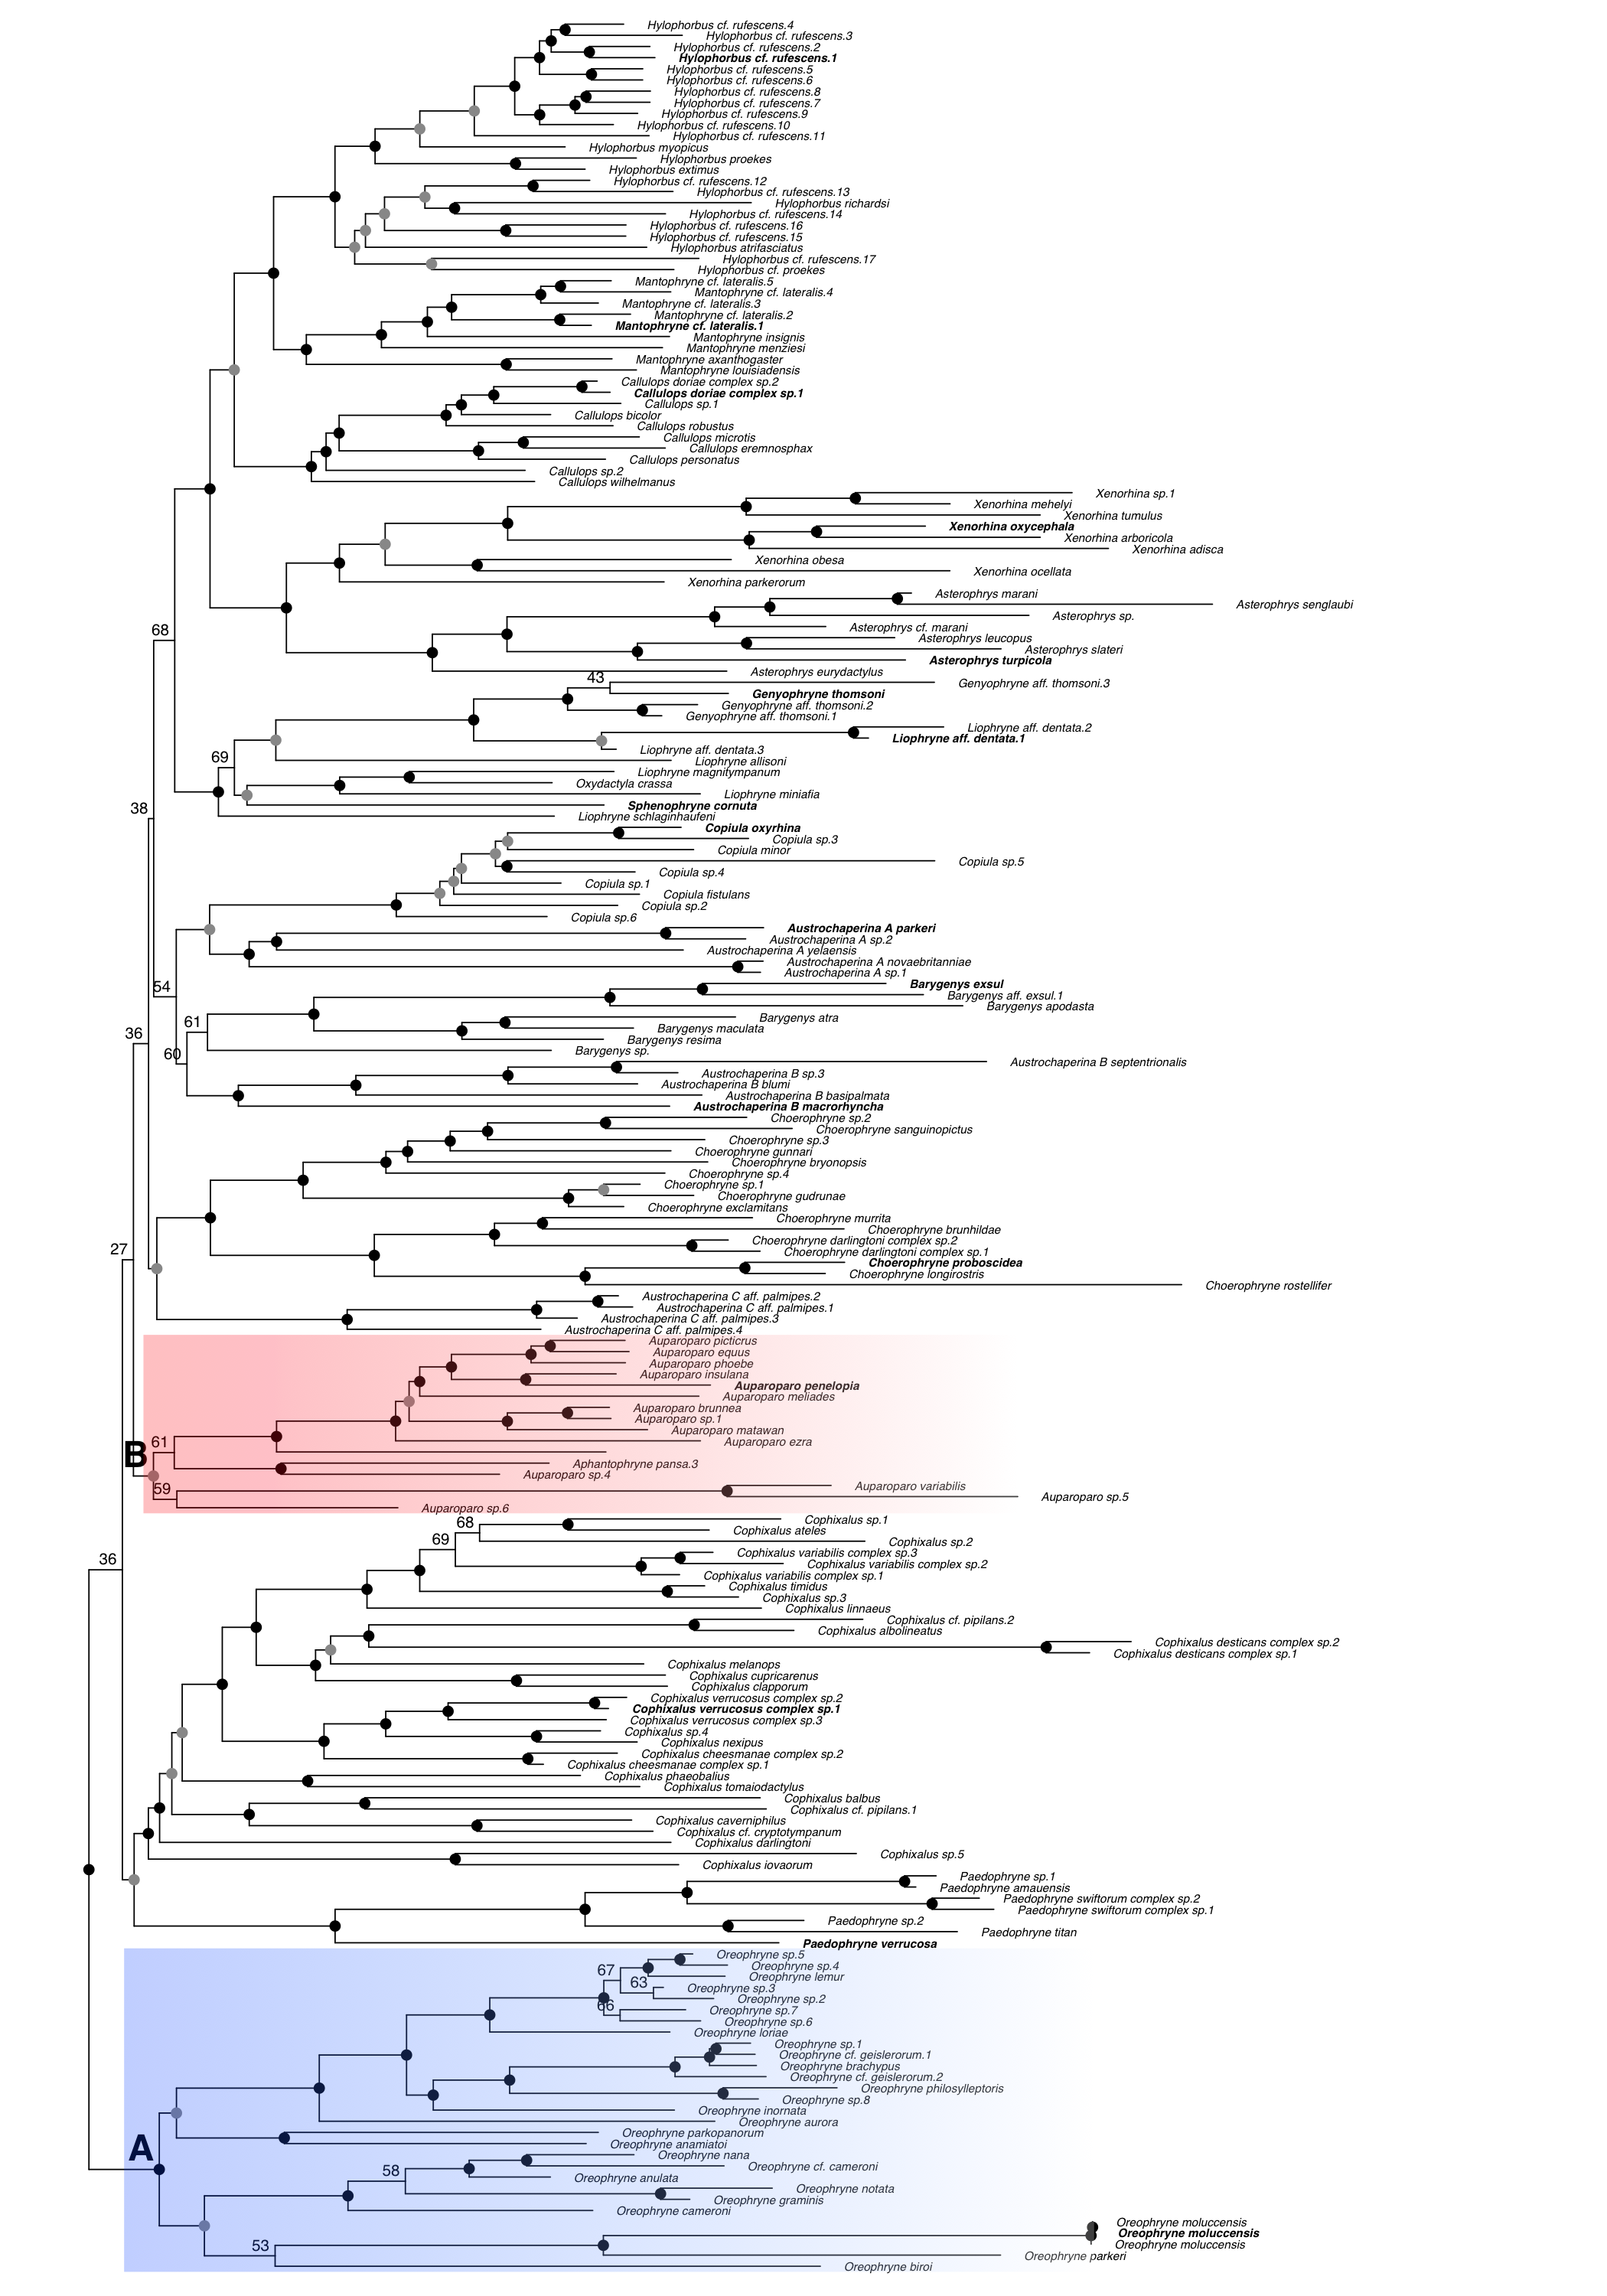
\includegraphics[keepaspectratio]{../Results/fig2.FullTree_support_highlight.png}}

}

\caption{\label{fig-phylo}Molecular phyogenetic hypothesis of
Asterophryinae showing polyphyly of \emph{Oreophryne} sensu lato, into
two reciprocally monophyletic clades that are not sister taxa. Node A is
\emph{Oreophryne} (blue clade) and node B is \emph{Auparoparo} (red
clade) based on the position of the type species \emph{Oreophryne
senkenbergiana}. Nodal support: black dots indicate ML boostrap support
\textgreater= 95\%, grey dots \textgreater= 75\%, numeric values given
for nodes below 75\% support. Outgroup taxa excluded. Taxa in bold are
the type species for each genus (or a proxy species used as an internal
reference).}

\end{figure}%

\subsection{Morphology, Behavior, and Ranked
Taxonomy}\label{morphology-behavior-and-ranked-taxonomy}

We find no morphological synapomorphies that distinguish
\emph{Auparoparo} from \emph{Oreophryne}. \emph{Oreophryne} sensu lato
is diagnosed by characters of the pectoral girdle: posessing highly
reduced, curved procoracoid cartilages and clavicles, and lacking an
omosternum (Parker, 1934; Zweifel, 2003). We found that this suite of
characters is present in both \emph{Oreophryne} and \emph{Auparoparo},
and therefore is not diagnostic for either \emph{Oreophryne} or
\emph{Auparoparo} (Table~\ref{tbl-morph}).

Two traits imperfectly segregate between the clades, relative finger and
toe pad widths and call type (Table~\ref{tbl-morph}), which may assist
in preliminary identification. Both \emph{Oreophryne} and
\emph{Auparoparo} are arboreal clades with expanded digital pads.
Whereas \emph{Oreophryne} have finger and toe pads of roughly equal
width, \emph{Auparoparo} have visibly larger finger pads, with finger
pads roughly 20-30\% wider than toes. Both \emph{Oreophryne} and
\emph{Auparoparo} use a variety of call types, with ``honks'' or
``peeps'' used only by \emph{Oreophryne}, whereas ``whinny'' calls are
used only by \emph{Auparoparo}. A minority of species in both groups use
the ``rattle'' call type. However, both toe pad width and call type are
variable traits with some overlap and thus not unambiguosly diagnostic.
Furthermore, possesssion of expanded digital pads is clearly an adaptive
trait for arboreality and prone to homoplasy.

\global\setlength{\Oldarrayrulewidth}{\arrayrulewidth}

\global\setlength{\Oldtabcolsep}{\tabcolsep}

\setlength{\tabcolsep}{2pt}

\renewcommand*{\arraystretch}{1.5}



\providecommand{\ascline}[3]{\noalign{\global\arrayrulewidth #1}\arrayrulecolor[HTML]{#2}\cline{#3}}

\begin{longtable}[c]{|p{0.98in}|p{1.18in}|p{0.47in}|p{0.45in}|p{0.47in}|p{0.43in}|p{1.39in}|p{1.12in}|p{0.62in}|p{0.85in}|p{0.71in}|p{1.17in}|p{2.28in}}

\caption{\label{tbl-morph}Morphological character matrix.}

\tabularnewline

\ascline{1.5pt}{666666}{1-13}

\multicolumn{1}{>{\raggedright}m{\dimexpr 0.98in+0\tabcolsep}}{\advance\leftskip by 2.0pt\relax \advance\rightskip by 2.0pt\relax \textcolor[HTML]{666666}{\fontsize{11}{11}\selectfont{{\fontspec{Helvetica} \textbf{}}}}} & \multicolumn{1}{>{\raggedright}m{\dimexpr 1.18in+0\tabcolsep}}{\advance\leftskip by 2.0pt\relax \advance\rightskip by 2.0pt\relax \textcolor[HTML]{666666}{\fontsize{11}{11}\selectfont{{\fontspec{Helvetica} \textbf{}}}}} & \multicolumn{1}{>{\raggedright}m{\dimexpr 0.47in+0\tabcolsep}}{\advance\leftskip by 2.0pt\relax \advance\rightskip by 2.0pt\relax \textcolor[HTML]{666666}{\fontsize{11}{11}\selectfont{{\fontspec{Helvetica} \textbf{(1)}}}}} & \multicolumn{1}{>{\raggedright}m{\dimexpr 0.45in+0\tabcolsep}}{\advance\leftskip by 2.0pt\relax \advance\rightskip by 2.0pt\relax \textcolor[HTML]{666666}{\fontsize{11}{11}\selectfont{{\fontspec{Helvetica} \textbf{(2)}}}}} & \multicolumn{1}{>{\raggedright}m{\dimexpr 0.47in+0\tabcolsep}}{\advance\leftskip by 2.0pt\relax \advance\rightskip by 2.0pt\relax \textcolor[HTML]{666666}{\fontsize{11}{11}\selectfont{{\fontspec{Helvetica} \textbf{(3)}}}}} & \multicolumn{1}{>{\raggedright}m{\dimexpr 0.43in+0\tabcolsep}}{\advance\leftskip by 2.0pt\relax \advance\rightskip by 2.0pt\relax \textcolor[HTML]{666666}{\fontsize{11}{11}\selectfont{{\fontspec{Helvetica} \textbf{(4)}}}}} & \multicolumn{1}{>{\raggedright}m{\dimexpr 1.39in+0\tabcolsep}}{\advance\leftskip by 2.0pt\relax \advance\rightskip by 2.0pt\relax \textcolor[HTML]{666666}{\fontsize{11}{11}\selectfont{{\fontspec{Helvetica} \textbf{(5)}}}}} & \multicolumn{1}{>{\raggedright}m{\dimexpr 1.12in+0\tabcolsep}}{\advance\leftskip by 2.0pt\relax \advance\rightskip by 2.0pt\relax \textcolor[HTML]{666666}{\fontsize{11}{11}\selectfont{{\fontspec{Helvetica} \textbf{(6)}}}}} & \multicolumn{1}{>{\raggedright}m{\dimexpr 0.62in+0\tabcolsep}}{\advance\leftskip by 2.0pt\relax \advance\rightskip by 2.0pt\relax \textcolor[HTML]{666666}{\fontsize{11}{11}\selectfont{{\fontspec{Helvetica} \textbf{(7)}}}}} & \multicolumn{1}{>{\raggedright}m{\dimexpr 0.85in+0\tabcolsep}}{\advance\leftskip by 2.0pt\relax \advance\rightskip by 2.0pt\relax \textcolor[HTML]{666666}{\fontsize{11}{11}\selectfont{{\fontspec{Helvetica} \textbf{(8)}}}}} & \multicolumn{1}{>{\raggedright}m{\dimexpr 0.71in+0\tabcolsep}}{\advance\leftskip by 2.0pt\relax \advance\rightskip by 2.0pt\relax \textcolor[HTML]{666666}{\fontsize{11}{11}\selectfont{{\fontspec{Helvetica} \textbf{(9)}}}}} & \multicolumn{1}{>{\raggedright}m{\dimexpr 1.17in+0\tabcolsep}}{\advance\leftskip by 2.0pt\relax \advance\rightskip by 2.0pt\relax \textcolor[HTML]{666666}{\fontsize{11}{11}\selectfont{{\fontspec{Helvetica} \textbf{(10)}}}}} & \multicolumn{1}{>{\raggedright}m{\dimexpr 2.28in+0\tabcolsep}}{\advance\leftskip by 2.0pt\relax \advance\rightskip by 2.0pt\relax \textcolor[HTML]{666666}{\fontsize{11}{11}\selectfont{{\fontspec{Helvetica} \textbf{(11)}}}}} \\





\multicolumn{1}{>{\raggedright}m{\dimexpr 0.98in+0\tabcolsep}}{\advance\leftskip by 2.0pt\relax \advance\rightskip by 2.0pt\relax \textcolor[HTML]{666666}{\fontsize{11}{11}\selectfont{{\fontspec{Helvetica} \textbf{Genus}}}}} & \multicolumn{1}{>{\raggedright}m{\dimexpr 1.18in+0\tabcolsep}}{\advance\leftskip by 2.0pt\relax \advance\rightskip by 2.0pt\relax \textcolor[HTML]{666666}{\fontsize{11}{11}\selectfont{{\fontspec{Helvetica} \textbf{species}}}}} & \multicolumn{1}{>{\raggedright}m{\dimexpr 0.47in+0\tabcolsep}}{\advance\leftskip by 2.0pt\relax \advance\rightskip by 2.0pt\relax \textcolor[HTML]{666666}{\fontsize{11}{11}\selectfont{{\fontspec{Helvetica} \textbf{proc}}}}} & \multicolumn{1}{>{\raggedright}m{\dimexpr 0.45in+0\tabcolsep}}{\advance\leftskip by 2.0pt\relax \advance\rightskip by 2.0pt\relax \textcolor[HTML]{666666}{\fontsize{11}{11}\selectfont{{\fontspec{Helvetica} \textbf{clav}}}}} & \multicolumn{1}{>{\raggedright}m{\dimexpr 0.47in+0\tabcolsep}}{\advance\leftskip by 2.0pt\relax \advance\rightskip by 2.0pt\relax \textcolor[HTML]{666666}{\fontsize{11}{11}\selectfont{{\fontspec{Helvetica} \textbf{omo}}}}} & \multicolumn{1}{>{\raggedright}m{\dimexpr 0.43in+0\tabcolsep}}{\advance\leftskip by 2.0pt\relax \advance\rightskip by 2.0pt\relax \textcolor[HTML]{666666}{\fontsize{11}{11}\selectfont{{\fontspec{Helvetica} \textbf{ster}}}}} & \multicolumn{1}{>{\raggedright}m{\dimexpr 1.39in+0\tabcolsep}}{\advance\leftskip by 2.0pt\relax \advance\rightskip by 2.0pt\relax \textcolor[HTML]{666666}{\fontsize{11}{11}\selectfont{{\fontspec{Helvetica} \textbf{call\ type}}}}} & \multicolumn{1}{>{\raggedright}m{\dimexpr 1.12in+0\tabcolsep}}{\advance\leftskip by 2.0pt\relax \advance\rightskip by 2.0pt\relax \textcolor[HTML]{666666}{\fontsize{11}{11}\selectfont{{\fontspec{Helvetica} \textbf{fing:\ toe\ width}}}}} & \multicolumn{1}{>{\raggedright}m{\dimexpr 0.62in+0\tabcolsep}}{\advance\leftskip by 2.0pt\relax \advance\rightskip by 2.0pt\relax \textcolor[HTML]{666666}{\fontsize{11}{11}\selectfont{{\fontspec{Helvetica} \textbf{pec\ lig}}}}} & \multicolumn{1}{>{\raggedright}m{\dimexpr 0.85in+0\tabcolsep}}{\advance\leftskip by 2.0pt\relax \advance\rightskip by 2.0pt\relax \textcolor[HTML]{666666}{\fontsize{11}{11}\selectfont{{\fontspec{Helvetica} \textbf{rel\ toe\ len}}}}} & \multicolumn{1}{>{\raggedright}m{\dimexpr 0.71in+0\tabcolsep}}{\advance\leftskip by 2.0pt\relax \advance\rightskip by 2.0pt\relax \textcolor[HTML]{666666}{\fontsize{11}{11}\selectfont{{\fontspec{Helvetica} \textbf{toe\ web}}}}} & \multicolumn{1}{>{\raggedright}m{\dimexpr 1.17in+0\tabcolsep}}{\advance\leftskip by 2.0pt\relax \advance\rightskip by 2.0pt\relax \textcolor[HTML]{666666}{\fontsize{11}{11}\selectfont{{\fontspec{Helvetica} \textbf{tymp:eye\ diam}}}}} & \multicolumn{1}{>{\raggedright}m{\dimexpr 2.28in+0\tabcolsep}}{\advance\leftskip by 2.0pt\relax \advance\rightskip by 2.0pt\relax \textcolor[HTML]{666666}{\fontsize{11}{11}\selectfont{{\fontspec{Helvetica} \textbf{character\ data\ reference}}}}} \\

\ascline{1.5pt}{666666}{1-13}\endfirsthead 

\ascline{1.5pt}{666666}{1-13}

\multicolumn{1}{>{\raggedright}m{\dimexpr 0.98in+0\tabcolsep}}{\advance\leftskip by 2.0pt\relax \advance\rightskip by 2.0pt\relax \textcolor[HTML]{666666}{\fontsize{11}{11}\selectfont{{\fontspec{Helvetica} \textbf{}}}}} & \multicolumn{1}{>{\raggedright}m{\dimexpr 1.18in+0\tabcolsep}}{\advance\leftskip by 2.0pt\relax \advance\rightskip by 2.0pt\relax \textcolor[HTML]{666666}{\fontsize{11}{11}\selectfont{{\fontspec{Helvetica} \textbf{}}}}} & \multicolumn{1}{>{\raggedright}m{\dimexpr 0.47in+0\tabcolsep}}{\advance\leftskip by 2.0pt\relax \advance\rightskip by 2.0pt\relax \textcolor[HTML]{666666}{\fontsize{11}{11}\selectfont{{\fontspec{Helvetica} \textbf{(1)}}}}} & \multicolumn{1}{>{\raggedright}m{\dimexpr 0.45in+0\tabcolsep}}{\advance\leftskip by 2.0pt\relax \advance\rightskip by 2.0pt\relax \textcolor[HTML]{666666}{\fontsize{11}{11}\selectfont{{\fontspec{Helvetica} \textbf{(2)}}}}} & \multicolumn{1}{>{\raggedright}m{\dimexpr 0.47in+0\tabcolsep}}{\advance\leftskip by 2.0pt\relax \advance\rightskip by 2.0pt\relax \textcolor[HTML]{666666}{\fontsize{11}{11}\selectfont{{\fontspec{Helvetica} \textbf{(3)}}}}} & \multicolumn{1}{>{\raggedright}m{\dimexpr 0.43in+0\tabcolsep}}{\advance\leftskip by 2.0pt\relax \advance\rightskip by 2.0pt\relax \textcolor[HTML]{666666}{\fontsize{11}{11}\selectfont{{\fontspec{Helvetica} \textbf{(4)}}}}} & \multicolumn{1}{>{\raggedright}m{\dimexpr 1.39in+0\tabcolsep}}{\advance\leftskip by 2.0pt\relax \advance\rightskip by 2.0pt\relax \textcolor[HTML]{666666}{\fontsize{11}{11}\selectfont{{\fontspec{Helvetica} \textbf{(5)}}}}} & \multicolumn{1}{>{\raggedright}m{\dimexpr 1.12in+0\tabcolsep}}{\advance\leftskip by 2.0pt\relax \advance\rightskip by 2.0pt\relax \textcolor[HTML]{666666}{\fontsize{11}{11}\selectfont{{\fontspec{Helvetica} \textbf{(6)}}}}} & \multicolumn{1}{>{\raggedright}m{\dimexpr 0.62in+0\tabcolsep}}{\advance\leftskip by 2.0pt\relax \advance\rightskip by 2.0pt\relax \textcolor[HTML]{666666}{\fontsize{11}{11}\selectfont{{\fontspec{Helvetica} \textbf{(7)}}}}} & \multicolumn{1}{>{\raggedright}m{\dimexpr 0.85in+0\tabcolsep}}{\advance\leftskip by 2.0pt\relax \advance\rightskip by 2.0pt\relax \textcolor[HTML]{666666}{\fontsize{11}{11}\selectfont{{\fontspec{Helvetica} \textbf{(8)}}}}} & \multicolumn{1}{>{\raggedright}m{\dimexpr 0.71in+0\tabcolsep}}{\advance\leftskip by 2.0pt\relax \advance\rightskip by 2.0pt\relax \textcolor[HTML]{666666}{\fontsize{11}{11}\selectfont{{\fontspec{Helvetica} \textbf{(9)}}}}} & \multicolumn{1}{>{\raggedright}m{\dimexpr 1.17in+0\tabcolsep}}{\advance\leftskip by 2.0pt\relax \advance\rightskip by 2.0pt\relax \textcolor[HTML]{666666}{\fontsize{11}{11}\selectfont{{\fontspec{Helvetica} \textbf{(10)}}}}} & \multicolumn{1}{>{\raggedright}m{\dimexpr 2.28in+0\tabcolsep}}{\advance\leftskip by 2.0pt\relax \advance\rightskip by 2.0pt\relax \textcolor[HTML]{666666}{\fontsize{11}{11}\selectfont{{\fontspec{Helvetica} \textbf{(11)}}}}} \\





\multicolumn{1}{>{\raggedright}m{\dimexpr 0.98in+0\tabcolsep}}{\advance\leftskip by 2.0pt\relax \advance\rightskip by 2.0pt\relax \textcolor[HTML]{666666}{\fontsize{11}{11}\selectfont{{\fontspec{Helvetica} \textbf{Genus}}}}} & \multicolumn{1}{>{\raggedright}m{\dimexpr 1.18in+0\tabcolsep}}{\advance\leftskip by 2.0pt\relax \advance\rightskip by 2.0pt\relax \textcolor[HTML]{666666}{\fontsize{11}{11}\selectfont{{\fontspec{Helvetica} \textbf{species}}}}} & \multicolumn{1}{>{\raggedright}m{\dimexpr 0.47in+0\tabcolsep}}{\advance\leftskip by 2.0pt\relax \advance\rightskip by 2.0pt\relax \textcolor[HTML]{666666}{\fontsize{11}{11}\selectfont{{\fontspec{Helvetica} \textbf{proc}}}}} & \multicolumn{1}{>{\raggedright}m{\dimexpr 0.45in+0\tabcolsep}}{\advance\leftskip by 2.0pt\relax \advance\rightskip by 2.0pt\relax \textcolor[HTML]{666666}{\fontsize{11}{11}\selectfont{{\fontspec{Helvetica} \textbf{clav}}}}} & \multicolumn{1}{>{\raggedright}m{\dimexpr 0.47in+0\tabcolsep}}{\advance\leftskip by 2.0pt\relax \advance\rightskip by 2.0pt\relax \textcolor[HTML]{666666}{\fontsize{11}{11}\selectfont{{\fontspec{Helvetica} \textbf{omo}}}}} & \multicolumn{1}{>{\raggedright}m{\dimexpr 0.43in+0\tabcolsep}}{\advance\leftskip by 2.0pt\relax \advance\rightskip by 2.0pt\relax \textcolor[HTML]{666666}{\fontsize{11}{11}\selectfont{{\fontspec{Helvetica} \textbf{ster}}}}} & \multicolumn{1}{>{\raggedright}m{\dimexpr 1.39in+0\tabcolsep}}{\advance\leftskip by 2.0pt\relax \advance\rightskip by 2.0pt\relax \textcolor[HTML]{666666}{\fontsize{11}{11}\selectfont{{\fontspec{Helvetica} \textbf{call\ type}}}}} & \multicolumn{1}{>{\raggedright}m{\dimexpr 1.12in+0\tabcolsep}}{\advance\leftskip by 2.0pt\relax \advance\rightskip by 2.0pt\relax \textcolor[HTML]{666666}{\fontsize{11}{11}\selectfont{{\fontspec{Helvetica} \textbf{fing:\ toe\ width}}}}} & \multicolumn{1}{>{\raggedright}m{\dimexpr 0.62in+0\tabcolsep}}{\advance\leftskip by 2.0pt\relax \advance\rightskip by 2.0pt\relax \textcolor[HTML]{666666}{\fontsize{11}{11}\selectfont{{\fontspec{Helvetica} \textbf{pec\ lig}}}}} & \multicolumn{1}{>{\raggedright}m{\dimexpr 0.85in+0\tabcolsep}}{\advance\leftskip by 2.0pt\relax \advance\rightskip by 2.0pt\relax \textcolor[HTML]{666666}{\fontsize{11}{11}\selectfont{{\fontspec{Helvetica} \textbf{rel\ toe\ len}}}}} & \multicolumn{1}{>{\raggedright}m{\dimexpr 0.71in+0\tabcolsep}}{\advance\leftskip by 2.0pt\relax \advance\rightskip by 2.0pt\relax \textcolor[HTML]{666666}{\fontsize{11}{11}\selectfont{{\fontspec{Helvetica} \textbf{toe\ web}}}}} & \multicolumn{1}{>{\raggedright}m{\dimexpr 1.17in+0\tabcolsep}}{\advance\leftskip by 2.0pt\relax \advance\rightskip by 2.0pt\relax \textcolor[HTML]{666666}{\fontsize{11}{11}\selectfont{{\fontspec{Helvetica} \textbf{tymp:eye\ diam}}}}} & \multicolumn{1}{>{\raggedright}m{\dimexpr 2.28in+0\tabcolsep}}{\advance\leftskip by 2.0pt\relax \advance\rightskip by 2.0pt\relax \textcolor[HTML]{666666}{\fontsize{11}{11}\selectfont{{\fontspec{Helvetica} \textbf{character\ data\ reference}}}}} \\

\ascline{1.5pt}{666666}{1-13}\endhead



\multicolumn{13}{>{\raggedright}m{\dimexpr 12.1in+24\tabcolsep}}{\advance\leftskip by 2.0pt\relax \advance\rightskip by 2.0pt\relax \textcolor[HTML]{666666}{\fontsize{11}{11}\selectfont{{\fontspec{Helvetica} \textsuperscript{1}}}}\textcolor[HTML]{666666}{\fontsize{11}{11}\selectfont{{\fontspec{Helvetica} Character\ states\ obtained\ from\ the\ literature,\ specimens\ not\ available\ for\ examination\ in\ this\ study.}}}} \\





\multicolumn{13}{>{\raggedright}m{\dimexpr 12.1in+24\tabcolsep}}{\advance\leftskip by 2.0pt\relax \advance\rightskip by 2.0pt\relax \textcolor[HTML]{666666}{\fontsize{11}{11}\selectfont{{\fontspec{Helvetica} \textsuperscript{2}}}}\textcolor[HTML]{666666}{\fontsize{11}{11}\selectfont{{\fontspec{Helvetica} Hill\ et\ al.\ 2022\ places\ }}}\textcolor[HTML]{666666}{\fontsize{11}{11}\selectfont{{\fontspec{Helvetica} \textit{Aphantophryne\ pansa}}}}\textcolor[HTML]{666666}{\fontsize{11}{11}\selectfont{{\fontspec{Helvetica} \ within\ }}}\textcolor[HTML]{666666}{\fontsize{11}{11}\selectfont{{\fontspec{Helvetica} \textit{Auparoparo}}}}\textcolor[HTML]{666666}{\fontsize{11}{11}\selectfont{{\fontspec{Helvetica} ,\ but\ the\ status\ of\ }}}\textcolor[HTML]{666666}{\fontsize{11}{11}\selectfont{{\fontspec{Helvetica} \textit{Aphantophryne}}}}\textcolor[HTML]{666666}{\fontsize{11}{11}\selectfont{{\fontspec{Helvetica} \ requires\ further\ study\ with\ samples\ from\ additional\ species\ and\ localities.}}}} \\





\multicolumn{13}{>{\raggedright}m{\dimexpr 12.1in+24\tabcolsep}}{\advance\leftskip by 2.0pt\relax \advance\rightskip by 2.0pt\relax \textcolor[HTML]{666666}{\fontsize{11}{11}\selectfont{{\fontspec{Helvetica} *External\ characters\ were\ examined\ from\ specimens,\ internal\ characters\ and\ pupil\ shape\ taken\ from\ the\ literature.}}}} \\

\endlastfoot



\multicolumn{1}{>{\raggedright}p{\dimexpr 0.98in+0\tabcolsep}}{\advance\leftskip by 2.0pt\relax \advance\rightskip by 2.0pt\relax \textcolor[HTML]{666666}{\fontsize{11}{11}\selectfont{{\fontspec{Helvetica} \textit{Oreophryne}}}}} & \multicolumn{1}{>{\raggedright}m{\dimexpr 1.18in+0\tabcolsep}}{\advance\leftskip by 2.0pt\relax \advance\rightskip by 2.0pt\relax \textcolor[HTML]{666666}{\fontsize{11}{11}\selectfont{{\fontspec{Helvetica} \textit{anamiatoi}}}}} & \multicolumn{1}{>{\raggedright}m{\dimexpr 0.47in+0\tabcolsep}}{\advance\leftskip by 2.0pt\relax \advance\rightskip by 2.0pt\relax \textcolor[HTML]{666666}{\fontsize{11}{11}\selectfont{{\fontspec{Helvetica} CR}}}} & \multicolumn{1}{>{\raggedright}m{\dimexpr 0.45in+0\tabcolsep}}{\advance\leftskip by 2.0pt\relax \advance\rightskip by 2.0pt\relax \textcolor[HTML]{666666}{\fontsize{11}{11}\selectfont{{\fontspec{Helvetica} CR}}}} & \multicolumn{1}{>{\raggedright}m{\dimexpr 0.47in+0\tabcolsep}}{\advance\leftskip by 2.0pt\relax \advance\rightskip by 2.0pt\relax \textcolor[HTML]{666666}{\fontsize{11}{11}\selectfont{{\fontspec{Helvetica} –}}}} & \multicolumn{1}{>{\raggedright}m{\dimexpr 0.43in+0\tabcolsep}}{\advance\leftskip by 2.0pt\relax \advance\rightskip by 2.0pt\relax \textcolor[HTML]{666666}{\fontsize{11}{11}\selectfont{{\fontspec{Helvetica} cart}}}} & \multicolumn{1}{>{\raggedright}m{\dimexpr 1.39in+0\tabcolsep}}{\advance\leftskip by 2.0pt\relax \advance\rightskip by 2.0pt\relax \textcolor[HTML]{666666}{\fontsize{11}{11}\selectfont{{\fontspec{Helvetica} \ chuckle\ or\ cackle}}}} & \multicolumn{1}{>{\raggedright}m{\dimexpr 1.12in+0\tabcolsep}}{\advance\leftskip by 2.0pt\relax \advance\rightskip by 2.0pt\relax \textcolor[HTML]{666666}{\fontsize{11}{11}\selectfont{{\fontspec{Helvetica} 1.2}}}} & \multicolumn{1}{>{\raggedright}m{\dimexpr 0.62in+0\tabcolsep}}{\advance\leftskip by 2.0pt\relax \advance\rightskip by 2.0pt\relax \textcolor[HTML]{666666}{\fontsize{11}{11}\selectfont{{\fontspec{Helvetica} cart}}}} & \multicolumn{1}{>{\raggedright}m{\dimexpr 0.85in+0\tabcolsep}}{\advance\leftskip by 2.0pt\relax \advance\rightskip by 2.0pt\relax \textcolor[HTML]{666666}{\fontsize{11}{11}\selectfont{{\fontspec{Helvetica} 5>3}}}} & \multicolumn{1}{>{\raggedright}m{\dimexpr 0.71in+0\tabcolsep}}{\advance\leftskip by 2.0pt\relax \advance\rightskip by 2.0pt\relax \textcolor[HTML]{666666}{\fontsize{11}{11}\selectfont{{\fontspec{Helvetica} –}}}} & \multicolumn{1}{>{\raggedright}m{\dimexpr 1.17in+0\tabcolsep}}{\advance\leftskip by 2.0pt\relax \advance\rightskip by 2.0pt\relax \textcolor[HTML]{666666}{\fontsize{11}{11}\selectfont{{\fontspec{Helvetica} 1/4}}}} & \multicolumn{1}{>{\raggedright}m{\dimexpr 2.28in+0\tabcolsep}}{\advance\leftskip by 2.0pt\relax \advance\rightskip by 2.0pt\relax \textcolor[HTML]{666666}{\fontsize{11}{11}\selectfont{{\fontspec{Helvetica} Kraus\ Allison\ 2009}}}} \\





\multicolumn{1}{>{\raggedright}p{\dimexpr 0.98in+0\tabcolsep}}{} & \multicolumn{1}{>{\raggedright}m{\dimexpr 1.18in+0\tabcolsep}}{\advance\leftskip by 2.0pt\relax \advance\rightskip by 2.0pt\relax \textcolor[HTML]{666666}{\fontsize{11}{11}\selectfont{{\fontspec{Helvetica} \textit{anulata}}}}\textcolor[HTML]{666666}{\fontsize{11}{11}\selectfont{{\fontspec{Helvetica} \textit{\textsuperscript{1}}}}}} & \multicolumn{1}{>{\raggedright}m{\dimexpr 0.47in+0\tabcolsep}}{\advance\leftskip by 2.0pt\relax \advance\rightskip by 2.0pt\relax \textcolor[HTML]{666666}{\fontsize{11}{11}\selectfont{{\fontspec{Helvetica} CR}}}} & \multicolumn{1}{>{\raggedright}m{\dimexpr 0.45in+0\tabcolsep}}{\advance\leftskip by 2.0pt\relax \advance\rightskip by 2.0pt\relax \textcolor[HTML]{666666}{\fontsize{11}{11}\selectfont{{\fontspec{Helvetica} CR}}}} & \multicolumn{1}{>{\raggedright}m{\dimexpr 0.47in+0\tabcolsep}}{\advance\leftskip by 2.0pt\relax \advance\rightskip by 2.0pt\relax \textcolor[HTML]{666666}{\fontsize{11}{11}\selectfont{{\fontspec{Helvetica} –}}}} & \multicolumn{1}{>{\raggedright}m{\dimexpr 0.43in+0\tabcolsep}}{\advance\leftskip by 2.0pt\relax \advance\rightskip by 2.0pt\relax \textcolor[HTML]{666666}{\fontsize{11}{11}\selectfont{{\fontspec{Helvetica} cart}}}} & \multicolumn{1}{>{\raggedright}m{\dimexpr 1.39in+0\tabcolsep}}{\advance\leftskip by 2.0pt\relax \advance\rightskip by 2.0pt\relax \textcolor[HTML]{666666}{\fontsize{11}{11}\selectfont{{\fontspec{Helvetica} }}}} & \multicolumn{1}{>{\raggedright}m{\dimexpr 1.12in+0\tabcolsep}}{\advance\leftskip by 2.0pt\relax \advance\rightskip by 2.0pt\relax \textcolor[HTML]{666666}{\fontsize{11}{11}\selectfont{{\fontspec{Helvetica} slightly\ larger}}}} & \multicolumn{1}{>{\raggedright}m{\dimexpr 0.62in+0\tabcolsep}}{\advance\leftskip by 2.0pt\relax \advance\rightskip by 2.0pt\relax \textcolor[HTML]{666666}{\fontsize{11}{11}\selectfont{{\fontspec{Helvetica} }}}} & \multicolumn{1}{>{\raggedright}m{\dimexpr 0.85in+0\tabcolsep}}{\advance\leftskip by 2.0pt\relax \advance\rightskip by 2.0pt\relax \textcolor[HTML]{666666}{\fontsize{11}{11}\selectfont{{\fontspec{Helvetica} 5>3}}}} & \multicolumn{1}{>{\raggedright}m{\dimexpr 0.71in+0\tabcolsep}}{\advance\leftskip by 2.0pt\relax \advance\rightskip by 2.0pt\relax \textcolor[HTML]{666666}{\fontsize{11}{11}\selectfont{{\fontspec{Helvetica} –}}}} & \multicolumn{1}{>{\raggedright}m{\dimexpr 1.17in+0\tabcolsep}}{\advance\leftskip by 2.0pt\relax \advance\rightskip by 2.0pt\relax \textcolor[HTML]{666666}{\fontsize{11}{11}\selectfont{{\fontspec{Helvetica} 1/2}}}} & \multicolumn{1}{>{\raggedright}m{\dimexpr 2.28in+0\tabcolsep}}{\advance\leftskip by 2.0pt\relax \advance\rightskip by 2.0pt\relax \textcolor[HTML]{666666}{\fontsize{11}{11}\selectfont{{\fontspec{Helvetica} Stejneger\ 1908}}}} \\





\multicolumn{1}{>{\raggedright}p{\dimexpr 0.98in+0\tabcolsep}}{} & \multicolumn{1}{>{\raggedright}m{\dimexpr 1.18in+0\tabcolsep}}{\advance\leftskip by 2.0pt\relax \advance\rightskip by 2.0pt\relax \textcolor[HTML]{666666}{\fontsize{11}{11}\selectfont{{\fontspec{Helvetica} \textit{aurora}}}}} & \multicolumn{1}{>{\raggedright}m{\dimexpr 0.47in+0\tabcolsep}}{\advance\leftskip by 2.0pt\relax \advance\rightskip by 2.0pt\relax \textcolor[HTML]{666666}{\fontsize{11}{11}\selectfont{{\fontspec{Helvetica} CR}}}} & \multicolumn{1}{>{\raggedright}m{\dimexpr 0.45in+0\tabcolsep}}{\advance\leftskip by 2.0pt\relax \advance\rightskip by 2.0pt\relax \textcolor[HTML]{666666}{\fontsize{11}{11}\selectfont{{\fontspec{Helvetica} CR}}}} & \multicolumn{1}{>{\raggedright}m{\dimexpr 0.47in+0\tabcolsep}}{\advance\leftskip by 2.0pt\relax \advance\rightskip by 2.0pt\relax \textcolor[HTML]{666666}{\fontsize{11}{11}\selectfont{{\fontspec{Helvetica} –}}}} & \multicolumn{1}{>{\raggedright}m{\dimexpr 0.43in+0\tabcolsep}}{\advance\leftskip by 2.0pt\relax \advance\rightskip by 2.0pt\relax \textcolor[HTML]{666666}{\fontsize{11}{11}\selectfont{{\fontspec{Helvetica} cart}}}} & \multicolumn{1}{>{\raggedright}m{\dimexpr 1.39in+0\tabcolsep}}{\advance\leftskip by 2.0pt\relax \advance\rightskip by 2.0pt\relax \textcolor[HTML]{666666}{\fontsize{11}{11}\selectfont{{\fontspec{Helvetica} harsh\ croaks}}}} & \multicolumn{1}{>{\raggedright}m{\dimexpr 1.12in+0\tabcolsep}}{\advance\leftskip by 2.0pt\relax \advance\rightskip by 2.0pt\relax \textcolor[HTML]{666666}{\fontsize{11}{11}\selectfont{{\fontspec{Helvetica} }}}} & \multicolumn{1}{>{\raggedright}m{\dimexpr 0.62in+0\tabcolsep}}{\advance\leftskip by 2.0pt\relax \advance\rightskip by 2.0pt\relax \textcolor[HTML]{666666}{\fontsize{11}{11}\selectfont{{\fontspec{Helvetica} lig}}}} & \multicolumn{1}{>{\raggedright}m{\dimexpr 0.85in+0\tabcolsep}}{\advance\leftskip by 2.0pt\relax \advance\rightskip by 2.0pt\relax \textcolor[HTML]{666666}{\fontsize{11}{11}\selectfont{{\fontspec{Helvetica} 5>3}}}} & \multicolumn{1}{>{\raggedright}m{\dimexpr 0.71in+0\tabcolsep}}{\advance\leftskip by 2.0pt\relax \advance\rightskip by 2.0pt\relax \textcolor[HTML]{666666}{\fontsize{11}{11}\selectfont{{\fontspec{Helvetica} webbed}}}} & \multicolumn{1}{>{\raggedright}m{\dimexpr 1.17in+0\tabcolsep}}{\advance\leftskip by 2.0pt\relax \advance\rightskip by 2.0pt\relax \textcolor[HTML]{666666}{\fontsize{11}{11}\selectfont{{\fontspec{Helvetica} 1/4}}}} & \multicolumn{1}{>{\raggedright}m{\dimexpr 2.28in+0\tabcolsep}}{\advance\leftskip by 2.0pt\relax \advance\rightskip by 2.0pt\relax \textcolor[HTML]{666666}{\fontsize{11}{11}\selectfont{{\fontspec{Helvetica} Kraus\ 2016}}}} \\





\multicolumn{1}{>{\raggedright}p{\dimexpr 0.98in+0\tabcolsep}}{} & \multicolumn{1}{>{\raggedright}m{\dimexpr 1.18in+0\tabcolsep}}{\advance\leftskip by 2.0pt\relax \advance\rightskip by 2.0pt\relax \textcolor[HTML]{666666}{\fontsize{11}{11}\selectfont{{\fontspec{Helvetica} \textit{biroi}}}}} & \multicolumn{1}{>{\raggedright}m{\dimexpr 0.47in+0\tabcolsep}}{\advance\leftskip by 2.0pt\relax \advance\rightskip by 2.0pt\relax \textcolor[HTML]{666666}{\fontsize{11}{11}\selectfont{{\fontspec{Helvetica} CR}}}} & \multicolumn{1}{>{\raggedright}m{\dimexpr 0.45in+0\tabcolsep}}{\advance\leftskip by 2.0pt\relax \advance\rightskip by 2.0pt\relax \textcolor[HTML]{666666}{\fontsize{11}{11}\selectfont{{\fontspec{Helvetica} CR}}}} & \multicolumn{1}{>{\raggedright}m{\dimexpr 0.47in+0\tabcolsep}}{\advance\leftskip by 2.0pt\relax \advance\rightskip by 2.0pt\relax \textcolor[HTML]{666666}{\fontsize{11}{11}\selectfont{{\fontspec{Helvetica} –}}}} & \multicolumn{1}{>{\raggedright}m{\dimexpr 0.43in+0\tabcolsep}}{\advance\leftskip by 2.0pt\relax \advance\rightskip by 2.0pt\relax \textcolor[HTML]{666666}{\fontsize{11}{11}\selectfont{{\fontspec{Helvetica} cart}}}} & \multicolumn{1}{>{\raggedright}m{\dimexpr 1.39in+0\tabcolsep}}{\advance\leftskip by 2.0pt\relax \advance\rightskip by 2.0pt\relax \textcolor[HTML]{666666}{\fontsize{11}{11}\selectfont{{\fontspec{Helvetica} rattle}}}} & \multicolumn{1}{>{\raggedright}m{\dimexpr 1.12in+0\tabcolsep}}{\advance\leftskip by 2.0pt\relax \advance\rightskip by 2.0pt\relax \textcolor[HTML]{666666}{\fontsize{11}{11}\selectfont{{\fontspec{Helvetica} 1.1}}}} & \multicolumn{1}{>{\raggedright}m{\dimexpr 0.62in+0\tabcolsep}}{\advance\leftskip by 2.0pt\relax \advance\rightskip by 2.0pt\relax \textcolor[HTML]{666666}{\fontsize{11}{11}\selectfont{{\fontspec{Helvetica} lig}}}} & \multicolumn{1}{>{\raggedright}m{\dimexpr 0.85in+0\tabcolsep}}{\advance\leftskip by 2.0pt\relax \advance\rightskip by 2.0pt\relax \textcolor[HTML]{666666}{\fontsize{11}{11}\selectfont{{\fontspec{Helvetica} 5=3}}}} & \multicolumn{1}{>{\raggedright}m{\dimexpr 0.71in+0\tabcolsep}}{\advance\leftskip by 2.0pt\relax \advance\rightskip by 2.0pt\relax \textcolor[HTML]{666666}{\fontsize{11}{11}\selectfont{{\fontspec{Helvetica} webbed}}}} & \multicolumn{1}{>{\raggedright}m{\dimexpr 1.17in+0\tabcolsep}}{\advance\leftskip by 2.0pt\relax \advance\rightskip by 2.0pt\relax \textcolor[HTML]{666666}{\fontsize{11}{11}\selectfont{{\fontspec{Helvetica} 1/4}}}} & \multicolumn{1}{>{\raggedright}m{\dimexpr 2.28in+0\tabcolsep}}{\advance\leftskip by 2.0pt\relax \advance\rightskip by 2.0pt\relax \textcolor[HTML]{666666}{\fontsize{11}{11}\selectfont{{\fontspec{Helvetica} Zweifel\ et\ al.\ 2003}}}} \\





\multicolumn{1}{>{\raggedright}p{\dimexpr 0.98in+0\tabcolsep}}{} & \multicolumn{1}{>{\raggedright}m{\dimexpr 1.18in+0\tabcolsep}}{\advance\leftskip by 2.0pt\relax \advance\rightskip by 2.0pt\relax \textcolor[HTML]{666666}{\fontsize{11}{11}\selectfont{{\fontspec{Helvetica} \textit{brachypus}}}}} & \multicolumn{1}{>{\raggedright}m{\dimexpr 0.47in+0\tabcolsep}}{\advance\leftskip by 2.0pt\relax \advance\rightskip by 2.0pt\relax \textcolor[HTML]{666666}{\fontsize{11}{11}\selectfont{{\fontspec{Helvetica} CR}}}} & \multicolumn{1}{>{\raggedright}m{\dimexpr 0.45in+0\tabcolsep}}{\advance\leftskip by 2.0pt\relax \advance\rightskip by 2.0pt\relax \textcolor[HTML]{666666}{\fontsize{11}{11}\selectfont{{\fontspec{Helvetica} CR}}}} & \multicolumn{1}{>{\raggedright}m{\dimexpr 0.47in+0\tabcolsep}}{\advance\leftskip by 2.0pt\relax \advance\rightskip by 2.0pt\relax \textcolor[HTML]{666666}{\fontsize{11}{11}\selectfont{{\fontspec{Helvetica} –}}}} & \multicolumn{1}{>{\raggedright}m{\dimexpr 0.43in+0\tabcolsep}}{\advance\leftskip by 2.0pt\relax \advance\rightskip by 2.0pt\relax \textcolor[HTML]{666666}{\fontsize{11}{11}\selectfont{{\fontspec{Helvetica} cart}}}} & \multicolumn{1}{>{\raggedright}m{\dimexpr 1.39in+0\tabcolsep}}{\advance\leftskip by 2.0pt\relax \advance\rightskip by 2.0pt\relax \textcolor[HTML]{666666}{\fontsize{11}{11}\selectfont{{\fontspec{Helvetica} long\ squeak}}}} & \multicolumn{1}{>{\raggedright}m{\dimexpr 1.12in+0\tabcolsep}}{\advance\leftskip by 2.0pt\relax \advance\rightskip by 2.0pt\relax \textcolor[HTML]{666666}{\fontsize{11}{11}\selectfont{{\fontspec{Helvetica} 1.1}}}} & \multicolumn{1}{>{\raggedright}m{\dimexpr 0.62in+0\tabcolsep}}{\advance\leftskip by 2.0pt\relax \advance\rightskip by 2.0pt\relax \textcolor[HTML]{666666}{\fontsize{11}{11}\selectfont{{\fontspec{Helvetica} lig}}}} & \multicolumn{1}{>{\raggedright}m{\dimexpr 0.85in+0\tabcolsep}}{\advance\leftskip by 2.0pt\relax \advance\rightskip by 2.0pt\relax \textcolor[HTML]{666666}{\fontsize{11}{11}\selectfont{{\fontspec{Helvetica} 5>3}}}} & \multicolumn{1}{>{\raggedright}m{\dimexpr 0.71in+0\tabcolsep}}{\advance\leftskip by 2.0pt\relax \advance\rightskip by 2.0pt\relax \textcolor[HTML]{666666}{\fontsize{11}{11}\selectfont{{\fontspec{Helvetica} webbed}}}} & \multicolumn{1}{>{\raggedright}m{\dimexpr 1.17in+0\tabcolsep}}{\advance\leftskip by 2.0pt\relax \advance\rightskip by 2.0pt\relax \textcolor[HTML]{666666}{\fontsize{11}{11}\selectfont{{\fontspec{Helvetica} 1/4}}}} & \multicolumn{1}{>{\raggedright}m{\dimexpr 2.28in+0\tabcolsep}}{\advance\leftskip by 2.0pt\relax \advance\rightskip by 2.0pt\relax \textcolor[HTML]{666666}{\fontsize{11}{11}\selectfont{{\fontspec{Helvetica} Zweifel\ et\ al.\ 2003}}}} \\





\multicolumn{1}{>{\raggedright}p{\dimexpr 0.98in+0\tabcolsep}}{} & \multicolumn{1}{>{\raggedright}m{\dimexpr 1.18in+0\tabcolsep}}{\advance\leftskip by 2.0pt\relax \advance\rightskip by 2.0pt\relax \textcolor[HTML]{666666}{\fontsize{11}{11}\selectfont{{\fontspec{Helvetica} \textit{cameroni}}}}} & \multicolumn{1}{>{\raggedright}m{\dimexpr 0.47in+0\tabcolsep}}{\advance\leftskip by 2.0pt\relax \advance\rightskip by 2.0pt\relax \textcolor[HTML]{666666}{\fontsize{11}{11}\selectfont{{\fontspec{Helvetica} CR}}}} & \multicolumn{1}{>{\raggedright}m{\dimexpr 0.45in+0\tabcolsep}}{\advance\leftskip by 2.0pt\relax \advance\rightskip by 2.0pt\relax \textcolor[HTML]{666666}{\fontsize{11}{11}\selectfont{{\fontspec{Helvetica} CR}}}} & \multicolumn{1}{>{\raggedright}m{\dimexpr 0.47in+0\tabcolsep}}{\advance\leftskip by 2.0pt\relax \advance\rightskip by 2.0pt\relax \textcolor[HTML]{666666}{\fontsize{11}{11}\selectfont{{\fontspec{Helvetica} –}}}} & \multicolumn{1}{>{\raggedright}m{\dimexpr 0.43in+0\tabcolsep}}{\advance\leftskip by 2.0pt\relax \advance\rightskip by 2.0pt\relax \textcolor[HTML]{666666}{\fontsize{11}{11}\selectfont{{\fontspec{Helvetica} cart}}}} & \multicolumn{1}{>{\raggedright}m{\dimexpr 1.39in+0\tabcolsep}}{\advance\leftskip by 2.0pt\relax \advance\rightskip by 2.0pt\relax \textcolor[HTML]{666666}{\fontsize{11}{11}\selectfont{{\fontspec{Helvetica} peep}}}} & \multicolumn{1}{>{\raggedright}m{\dimexpr 1.12in+0\tabcolsep}}{\advance\leftskip by 2.0pt\relax \advance\rightskip by 2.0pt\relax \textcolor[HTML]{666666}{\fontsize{11}{11}\selectfont{{\fontspec{Helvetica} }}}} & \multicolumn{1}{>{\raggedright}m{\dimexpr 0.62in+0\tabcolsep}}{\advance\leftskip by 2.0pt\relax \advance\rightskip by 2.0pt\relax \textcolor[HTML]{666666}{\fontsize{11}{11}\selectfont{{\fontspec{Helvetica} cart}}}} & \multicolumn{1}{>{\raggedright}m{\dimexpr 0.85in+0\tabcolsep}}{\advance\leftskip by 2.0pt\relax \advance\rightskip by 2.0pt\relax \textcolor[HTML]{666666}{\fontsize{11}{11}\selectfont{{\fontspec{Helvetica} 5>3}}}} & \multicolumn{1}{>{\raggedright}m{\dimexpr 0.71in+0\tabcolsep}}{\advance\leftskip by 2.0pt\relax \advance\rightskip by 2.0pt\relax \textcolor[HTML]{666666}{\fontsize{11}{11}\selectfont{{\fontspec{Helvetica} basal}}}} & \multicolumn{1}{>{\raggedright}m{\dimexpr 1.17in+0\tabcolsep}}{\advance\leftskip by 2.0pt\relax \advance\rightskip by 2.0pt\relax \textcolor[HTML]{666666}{\fontsize{11}{11}\selectfont{{\fontspec{Helvetica} 1/4}}}} & \multicolumn{1}{>{\raggedright}m{\dimexpr 2.28in+0\tabcolsep}}{\advance\leftskip by 2.0pt\relax \advance\rightskip by 2.0pt\relax \textcolor[HTML]{666666}{\fontsize{11}{11}\selectfont{{\fontspec{Helvetica} Kraus\ 2013}}}} \\





\multicolumn{1}{>{\raggedright}p{\dimexpr 0.98in+0\tabcolsep}}{} & \multicolumn{1}{>{\raggedright}m{\dimexpr 1.18in+0\tabcolsep}}{\advance\leftskip by 2.0pt\relax \advance\rightskip by 2.0pt\relax \textcolor[HTML]{666666}{\fontsize{11}{11}\selectfont{{\fontspec{Helvetica} \textit{frontifasciata}}}}\textcolor[HTML]{666666}{\fontsize{11}{11}\selectfont{{\fontspec{Helvetica} \textit{\textsuperscript{1}}}}}} & \multicolumn{1}{>{\raggedright}m{\dimexpr 0.47in+0\tabcolsep}}{\advance\leftskip by 2.0pt\relax \advance\rightskip by 2.0pt\relax \textcolor[HTML]{666666}{\fontsize{11}{11}\selectfont{{\fontspec{Helvetica} CR}}}} & \multicolumn{1}{>{\raggedright}m{\dimexpr 0.45in+0\tabcolsep}}{\advance\leftskip by 2.0pt\relax \advance\rightskip by 2.0pt\relax \textcolor[HTML]{666666}{\fontsize{11}{11}\selectfont{{\fontspec{Helvetica} CR}}}} & \multicolumn{1}{>{\raggedright}m{\dimexpr 0.47in+0\tabcolsep}}{\advance\leftskip by 2.0pt\relax \advance\rightskip by 2.0pt\relax \textcolor[HTML]{666666}{\fontsize{11}{11}\selectfont{{\fontspec{Helvetica} –}}}} & \multicolumn{1}{>{\raggedright}m{\dimexpr 0.43in+0\tabcolsep}}{\advance\leftskip by 2.0pt\relax \advance\rightskip by 2.0pt\relax \textcolor[HTML]{666666}{\fontsize{11}{11}\selectfont{{\fontspec{Helvetica} cart}}}} & \multicolumn{1}{>{\raggedright}m{\dimexpr 1.39in+0\tabcolsep}}{\advance\leftskip by 2.0pt\relax \advance\rightskip by 2.0pt\relax \textcolor[HTML]{666666}{\fontsize{11}{11}\selectfont{{\fontspec{Helvetica} }}}} & \multicolumn{1}{>{\raggedright}m{\dimexpr 1.12in+0\tabcolsep}}{\advance\leftskip by 2.0pt\relax \advance\rightskip by 2.0pt\relax \textcolor[HTML]{666666}{\fontsize{11}{11}\selectfont{{\fontspec{Helvetica} slightly\ larger}}}} & \multicolumn{1}{>{\raggedright}m{\dimexpr 0.62in+0\tabcolsep}}{\advance\leftskip by 2.0pt\relax \advance\rightskip by 2.0pt\relax \textcolor[HTML]{666666}{\fontsize{11}{11}\selectfont{{\fontspec{Helvetica} cart}}}} & \multicolumn{1}{>{\raggedright}m{\dimexpr 0.85in+0\tabcolsep}}{\advance\leftskip by 2.0pt\relax \advance\rightskip by 2.0pt\relax \textcolor[HTML]{666666}{\fontsize{11}{11}\selectfont{{\fontspec{Helvetica} 5>3}}}} & \multicolumn{1}{>{\raggedright}m{\dimexpr 0.71in+0\tabcolsep}}{\advance\leftskip by 2.0pt\relax \advance\rightskip by 2.0pt\relax \textcolor[HTML]{666666}{\fontsize{11}{11}\selectfont{{\fontspec{Helvetica} basal}}}} & \multicolumn{1}{>{\raggedright}m{\dimexpr 1.17in+0\tabcolsep}}{\advance\leftskip by 2.0pt\relax \advance\rightskip by 2.0pt\relax \textcolor[HTML]{666666}{\fontsize{11}{11}\selectfont{{\fontspec{Helvetica} 1/2}}}} & \multicolumn{1}{>{\raggedright}m{\dimexpr 2.28in+0\tabcolsep}}{\advance\leftskip by 2.0pt\relax \advance\rightskip by 2.0pt\relax \textcolor[HTML]{666666}{\fontsize{11}{11}\selectfont{{\fontspec{Helvetica} Horst\ 1883,\ Brongersma\ 1948}}}} \\





\multicolumn{1}{>{\raggedright}p{\dimexpr 0.98in+0\tabcolsep}}{} & \multicolumn{1}{>{\raggedright}m{\dimexpr 1.18in+0\tabcolsep}}{\advance\leftskip by 2.0pt\relax \advance\rightskip by 2.0pt\relax \textcolor[HTML]{666666}{\fontsize{11}{11}\selectfont{{\fontspec{Helvetica} \textit{geislerorum}}}}} & \multicolumn{1}{>{\raggedright}m{\dimexpr 0.47in+0\tabcolsep}}{\advance\leftskip by 2.0pt\relax \advance\rightskip by 2.0pt\relax \textcolor[HTML]{666666}{\fontsize{11}{11}\selectfont{{\fontspec{Helvetica} CR}}}} & \multicolumn{1}{>{\raggedright}m{\dimexpr 0.45in+0\tabcolsep}}{\advance\leftskip by 2.0pt\relax \advance\rightskip by 2.0pt\relax \textcolor[HTML]{666666}{\fontsize{11}{11}\selectfont{{\fontspec{Helvetica} CR}}}} & \multicolumn{1}{>{\raggedright}m{\dimexpr 0.47in+0\tabcolsep}}{\advance\leftskip by 2.0pt\relax \advance\rightskip by 2.0pt\relax \textcolor[HTML]{666666}{\fontsize{11}{11}\selectfont{{\fontspec{Helvetica} –}}}} & \multicolumn{1}{>{\raggedright}m{\dimexpr 0.43in+0\tabcolsep}}{\advance\leftskip by 2.0pt\relax \advance\rightskip by 2.0pt\relax \textcolor[HTML]{666666}{\fontsize{11}{11}\selectfont{{\fontspec{Helvetica} cart}}}} & \multicolumn{1}{>{\raggedright}m{\dimexpr 1.39in+0\tabcolsep}}{\advance\leftskip by 2.0pt\relax \advance\rightskip by 2.0pt\relax \textcolor[HTML]{666666}{\fontsize{11}{11}\selectfont{{\fontspec{Helvetica} rattle}}}} & \multicolumn{1}{>{\raggedright}m{\dimexpr 1.12in+0\tabcolsep}}{\advance\leftskip by 2.0pt\relax \advance\rightskip by 2.0pt\relax \textcolor[HTML]{666666}{\fontsize{11}{11}\selectfont{{\fontspec{Helvetica} }}}} & \multicolumn{1}{>{\raggedright}m{\dimexpr 0.62in+0\tabcolsep}}{\advance\leftskip by 2.0pt\relax \advance\rightskip by 2.0pt\relax \textcolor[HTML]{666666}{\fontsize{11}{11}\selectfont{{\fontspec{Helvetica} lig}}}} & \multicolumn{1}{>{\raggedright}m{\dimexpr 0.85in+0\tabcolsep}}{\advance\leftskip by 2.0pt\relax \advance\rightskip by 2.0pt\relax \textcolor[HTML]{666666}{\fontsize{11}{11}\selectfont{{\fontspec{Helvetica} 5>3}}}} & \multicolumn{1}{>{\raggedright}m{\dimexpr 0.71in+0\tabcolsep}}{\advance\leftskip by 2.0pt\relax \advance\rightskip by 2.0pt\relax \textcolor[HTML]{666666}{\fontsize{11}{11}\selectfont{{\fontspec{Helvetica} webbed}}}} & \multicolumn{1}{>{\raggedright}m{\dimexpr 1.17in+0\tabcolsep}}{\advance\leftskip by 2.0pt\relax \advance\rightskip by 2.0pt\relax \textcolor[HTML]{666666}{\fontsize{11}{11}\selectfont{{\fontspec{Helvetica} 1/3}}}} & \multicolumn{1}{>{\raggedright}m{\dimexpr 2.28in+0\tabcolsep}}{\advance\leftskip by 2.0pt\relax \advance\rightskip by 2.0pt\relax \textcolor[HTML]{666666}{\fontsize{11}{11}\selectfont{{\fontspec{Helvetica} Zweifel\ et\ al.\ 2003}}}} \\





\multicolumn{1}{>{\raggedright}p{\dimexpr 0.98in+0\tabcolsep}}{} & \multicolumn{1}{>{\raggedright}m{\dimexpr 1.18in+0\tabcolsep}}{\advance\leftskip by 2.0pt\relax \advance\rightskip by 2.0pt\relax \textcolor[HTML]{666666}{\fontsize{11}{11}\selectfont{{\fontspec{Helvetica} \textit{graminis}}}}\textcolor[HTML]{666666}{\fontsize{11}{11}\selectfont{{\fontspec{Helvetica} \textit{\textsuperscript{1}}}}}} & \multicolumn{1}{>{\raggedright}m{\dimexpr 0.47in+0\tabcolsep}}{\advance\leftskip by 2.0pt\relax \advance\rightskip by 2.0pt\relax \textcolor[HTML]{666666}{\fontsize{11}{11}\selectfont{{\fontspec{Helvetica} CR}}}} & \multicolumn{1}{>{\raggedright}m{\dimexpr 0.45in+0\tabcolsep}}{\advance\leftskip by 2.0pt\relax \advance\rightskip by 2.0pt\relax \textcolor[HTML]{666666}{\fontsize{11}{11}\selectfont{{\fontspec{Helvetica} CR}}}} & \multicolumn{1}{>{\raggedright}m{\dimexpr 0.47in+0\tabcolsep}}{\advance\leftskip by 2.0pt\relax \advance\rightskip by 2.0pt\relax \textcolor[HTML]{666666}{\fontsize{11}{11}\selectfont{{\fontspec{Helvetica} –}}}} & \multicolumn{1}{>{\raggedright}m{\dimexpr 0.43in+0\tabcolsep}}{\advance\leftskip by 2.0pt\relax \advance\rightskip by 2.0pt\relax \textcolor[HTML]{666666}{\fontsize{11}{11}\selectfont{{\fontspec{Helvetica} cart}}}} & \multicolumn{1}{>{\raggedright}m{\dimexpr 1.39in+0\tabcolsep}}{\advance\leftskip by 2.0pt\relax \advance\rightskip by 2.0pt\relax \textcolor[HTML]{666666}{\fontsize{11}{11}\selectfont{{\fontspec{Helvetica} peep}}}} & \multicolumn{1}{>{\raggedright}m{\dimexpr 1.12in+0\tabcolsep}}{\advance\leftskip by 2.0pt\relax \advance\rightskip by 2.0pt\relax \textcolor[HTML]{666666}{\fontsize{11}{11}\selectfont{{\fontspec{Helvetica} approx\ equal}}}} & \multicolumn{1}{>{\raggedright}m{\dimexpr 0.62in+0\tabcolsep}}{\advance\leftskip by 2.0pt\relax \advance\rightskip by 2.0pt\relax \textcolor[HTML]{666666}{\fontsize{11}{11}\selectfont{{\fontspec{Helvetica} cart}}}} & \multicolumn{1}{>{\raggedright}m{\dimexpr 0.85in+0\tabcolsep}}{\advance\leftskip by 2.0pt\relax \advance\rightskip by 2.0pt\relax \textcolor[HTML]{666666}{\fontsize{11}{11}\selectfont{{\fontspec{Helvetica} 5>3}}}} & \multicolumn{1}{>{\raggedright}m{\dimexpr 0.71in+0\tabcolsep}}{\advance\leftskip by 2.0pt\relax \advance\rightskip by 2.0pt\relax \textcolor[HTML]{666666}{\fontsize{11}{11}\selectfont{{\fontspec{Helvetica} –}}}} & \multicolumn{1}{>{\raggedright}m{\dimexpr 1.17in+0\tabcolsep}}{\advance\leftskip by 2.0pt\relax \advance\rightskip by 2.0pt\relax \textcolor[HTML]{666666}{\fontsize{11}{11}\selectfont{{\fontspec{Helvetica} 1/3}}}} & \multicolumn{1}{>{\raggedright}m{\dimexpr 2.28in+0\tabcolsep}}{\advance\leftskip by 2.0pt\relax \advance\rightskip by 2.0pt\relax \textcolor[HTML]{666666}{\fontsize{11}{11}\selectfont{{\fontspec{Helvetica} Gunther\ Richards\ 2012}}}} \\





\multicolumn{1}{>{\raggedright}p{\dimexpr 0.98in+0\tabcolsep}}{} & \multicolumn{1}{>{\raggedright}m{\dimexpr 1.18in+0\tabcolsep}}{\advance\leftskip by 2.0pt\relax \advance\rightskip by 2.0pt\relax \textcolor[HTML]{666666}{\fontsize{11}{11}\selectfont{{\fontspec{Helvetica} \textit{inornata}}}}} & \multicolumn{1}{>{\raggedright}m{\dimexpr 0.47in+0\tabcolsep}}{\advance\leftskip by 2.0pt\relax \advance\rightskip by 2.0pt\relax \textcolor[HTML]{666666}{\fontsize{11}{11}\selectfont{{\fontspec{Helvetica} CR}}}} & \multicolumn{1}{>{\raggedright}m{\dimexpr 0.45in+0\tabcolsep}}{\advance\leftskip by 2.0pt\relax \advance\rightskip by 2.0pt\relax \textcolor[HTML]{666666}{\fontsize{11}{11}\selectfont{{\fontspec{Helvetica} CR}}}} & \multicolumn{1}{>{\raggedright}m{\dimexpr 0.47in+0\tabcolsep}}{\advance\leftskip by 2.0pt\relax \advance\rightskip by 2.0pt\relax \textcolor[HTML]{666666}{\fontsize{11}{11}\selectfont{{\fontspec{Helvetica} –}}}} & \multicolumn{1}{>{\raggedright}m{\dimexpr 0.43in+0\tabcolsep}}{\advance\leftskip by 2.0pt\relax \advance\rightskip by 2.0pt\relax \textcolor[HTML]{666666}{\fontsize{11}{11}\selectfont{{\fontspec{Helvetica} cart}}}} & \multicolumn{1}{>{\raggedright}m{\dimexpr 1.39in+0\tabcolsep}}{\advance\leftskip by 2.0pt\relax \advance\rightskip by 2.0pt\relax \textcolor[HTML]{666666}{\fontsize{11}{11}\selectfont{{\fontspec{Helvetica} honk}}}} & \multicolumn{1}{>{\raggedright}m{\dimexpr 1.12in+0\tabcolsep}}{\advance\leftskip by 2.0pt\relax \advance\rightskip by 2.0pt\relax \textcolor[HTML]{666666}{\fontsize{11}{11}\selectfont{{\fontspec{Helvetica} 1.0}}}} & \multicolumn{1}{>{\raggedright}m{\dimexpr 0.62in+0\tabcolsep}}{\advance\leftskip by 2.0pt\relax \advance\rightskip by 2.0pt\relax \textcolor[HTML]{666666}{\fontsize{11}{11}\selectfont{{\fontspec{Helvetica} lig}}}} & \multicolumn{1}{>{\raggedright}m{\dimexpr 0.85in+0\tabcolsep}}{\advance\leftskip by 2.0pt\relax \advance\rightskip by 2.0pt\relax \textcolor[HTML]{666666}{\fontsize{11}{11}\selectfont{{\fontspec{Helvetica} 5>3}}}} & \multicolumn{1}{>{\raggedright}m{\dimexpr 0.71in+0\tabcolsep}}{\advance\leftskip by 2.0pt\relax \advance\rightskip by 2.0pt\relax \textcolor[HTML]{666666}{\fontsize{11}{11}\selectfont{{\fontspec{Helvetica} basal}}}} & \multicolumn{1}{>{\raggedright}m{\dimexpr 1.17in+0\tabcolsep}}{\advance\leftskip by 2.0pt\relax \advance\rightskip by 2.0pt\relax \textcolor[HTML]{666666}{\fontsize{11}{11}\selectfont{{\fontspec{Helvetica} 1/4}}}} & \multicolumn{1}{>{\raggedright}m{\dimexpr 2.28in+0\tabcolsep}}{\advance\leftskip by 2.0pt\relax \advance\rightskip by 2.0pt\relax \textcolor[HTML]{666666}{\fontsize{11}{11}\selectfont{{\fontspec{Helvetica} Kraus\ 2016}}}} \\





\multicolumn{1}{>{\raggedright}p{\dimexpr 0.98in+0\tabcolsep}}{} & \multicolumn{1}{>{\raggedright}m{\dimexpr 1.18in+0\tabcolsep}}{\advance\leftskip by 2.0pt\relax \advance\rightskip by 2.0pt\relax \textcolor[HTML]{666666}{\fontsize{11}{11}\selectfont{{\fontspec{Helvetica} \textit{lemur}}}}} & \multicolumn{1}{>{\raggedright}m{\dimexpr 0.47in+0\tabcolsep}}{\advance\leftskip by 2.0pt\relax \advance\rightskip by 2.0pt\relax \textcolor[HTML]{666666}{\fontsize{11}{11}\selectfont{{\fontspec{Helvetica} CR}}}} & \multicolumn{1}{>{\raggedright}m{\dimexpr 0.45in+0\tabcolsep}}{\advance\leftskip by 2.0pt\relax \advance\rightskip by 2.0pt\relax \textcolor[HTML]{666666}{\fontsize{11}{11}\selectfont{{\fontspec{Helvetica} CR}}}} & \multicolumn{1}{>{\raggedright}m{\dimexpr 0.47in+0\tabcolsep}}{\advance\leftskip by 2.0pt\relax \advance\rightskip by 2.0pt\relax \textcolor[HTML]{666666}{\fontsize{11}{11}\selectfont{{\fontspec{Helvetica} –}}}} & \multicolumn{1}{>{\raggedright}m{\dimexpr 0.43in+0\tabcolsep}}{\advance\leftskip by 2.0pt\relax \advance\rightskip by 2.0pt\relax \textcolor[HTML]{666666}{\fontsize{11}{11}\selectfont{{\fontspec{Helvetica} cart}}}} & \multicolumn{1}{>{\raggedright}m{\dimexpr 1.39in+0\tabcolsep}}{\advance\leftskip by 2.0pt\relax \advance\rightskip by 2.0pt\relax \textcolor[HTML]{666666}{\fontsize{11}{11}\selectfont{{\fontspec{Helvetica} honk}}}} & \multicolumn{1}{>{\raggedright}m{\dimexpr 1.12in+0\tabcolsep}}{\advance\leftskip by 2.0pt\relax \advance\rightskip by 2.0pt\relax \textcolor[HTML]{666666}{\fontsize{11}{11}\selectfont{{\fontspec{Helvetica} }}}} & \multicolumn{1}{>{\raggedright}m{\dimexpr 0.62in+0\tabcolsep}}{\advance\leftskip by 2.0pt\relax \advance\rightskip by 2.0pt\relax \textcolor[HTML]{666666}{\fontsize{11}{11}\selectfont{{\fontspec{Helvetica} lig}}}} & \multicolumn{1}{>{\raggedright}m{\dimexpr 0.85in+0\tabcolsep}}{\advance\leftskip by 2.0pt\relax \advance\rightskip by 2.0pt\relax \textcolor[HTML]{666666}{\fontsize{11}{11}\selectfont{{\fontspec{Helvetica} 5>3}}}} & \multicolumn{1}{>{\raggedright}m{\dimexpr 0.71in+0\tabcolsep}}{\advance\leftskip by 2.0pt\relax \advance\rightskip by 2.0pt\relax \textcolor[HTML]{666666}{\fontsize{11}{11}\selectfont{{\fontspec{Helvetica} basal}}}} & \multicolumn{1}{>{\raggedright}m{\dimexpr 1.17in+0\tabcolsep}}{\advance\leftskip by 2.0pt\relax \advance\rightskip by 2.0pt\relax \textcolor[HTML]{666666}{\fontsize{11}{11}\selectfont{{\fontspec{Helvetica} 1/4}}}} & \multicolumn{1}{>{\raggedright}m{\dimexpr 2.28in+0\tabcolsep}}{\advance\leftskip by 2.0pt\relax \advance\rightskip by 2.0pt\relax \textcolor[HTML]{666666}{\fontsize{11}{11}\selectfont{{\fontspec{Helvetica} Kraus\ 2016}}}} \\





\multicolumn{1}{>{\raggedright}p{\dimexpr 0.98in+0\tabcolsep}}{} & \multicolumn{1}{>{\raggedright}m{\dimexpr 1.18in+0\tabcolsep}}{\advance\leftskip by 2.0pt\relax \advance\rightskip by 2.0pt\relax \textcolor[HTML]{666666}{\fontsize{11}{11}\selectfont{{\fontspec{Helvetica} \textit{loriae}}}}} & \multicolumn{1}{>{\raggedright}m{\dimexpr 0.47in+0\tabcolsep}}{\advance\leftskip by 2.0pt\relax \advance\rightskip by 2.0pt\relax \textcolor[HTML]{666666}{\fontsize{11}{11}\selectfont{{\fontspec{Helvetica} CR}}}} & \multicolumn{1}{>{\raggedright}m{\dimexpr 0.45in+0\tabcolsep}}{\advance\leftskip by 2.0pt\relax \advance\rightskip by 2.0pt\relax \textcolor[HTML]{666666}{\fontsize{11}{11}\selectfont{{\fontspec{Helvetica} CR}}}} & \multicolumn{1}{>{\raggedright}m{\dimexpr 0.47in+0\tabcolsep}}{\advance\leftskip by 2.0pt\relax \advance\rightskip by 2.0pt\relax \textcolor[HTML]{666666}{\fontsize{11}{11}\selectfont{{\fontspec{Helvetica} –}}}} & \multicolumn{1}{>{\raggedright}m{\dimexpr 0.43in+0\tabcolsep}}{\advance\leftskip by 2.0pt\relax \advance\rightskip by 2.0pt\relax \textcolor[HTML]{666666}{\fontsize{11}{11}\selectfont{{\fontspec{Helvetica} cart}}}} & \multicolumn{1}{>{\raggedright}m{\dimexpr 1.39in+0\tabcolsep}}{\advance\leftskip by 2.0pt\relax \advance\rightskip by 2.0pt\relax \textcolor[HTML]{666666}{\fontsize{11}{11}\selectfont{{\fontspec{Helvetica} honk}}}} & \multicolumn{1}{>{\raggedright}m{\dimexpr 1.12in+0\tabcolsep}}{\advance\leftskip by 2.0pt\relax \advance\rightskip by 2.0pt\relax \textcolor[HTML]{666666}{\fontsize{11}{11}\selectfont{{\fontspec{Helvetica} }}}} & \multicolumn{1}{>{\raggedright}m{\dimexpr 0.62in+0\tabcolsep}}{\advance\leftskip by 2.0pt\relax \advance\rightskip by 2.0pt\relax \textcolor[HTML]{666666}{\fontsize{11}{11}\selectfont{{\fontspec{Helvetica} lig}}}} & \multicolumn{1}{>{\raggedright}m{\dimexpr 0.85in+0\tabcolsep}}{\advance\leftskip by 2.0pt\relax \advance\rightskip by 2.0pt\relax \textcolor[HTML]{666666}{\fontsize{11}{11}\selectfont{{\fontspec{Helvetica} 5>3}}}} & \multicolumn{1}{>{\raggedright}m{\dimexpr 0.71in+0\tabcolsep}}{\advance\leftskip by 2.0pt\relax \advance\rightskip by 2.0pt\relax \textcolor[HTML]{666666}{\fontsize{11}{11}\selectfont{{\fontspec{Helvetica} webbed}}}} & \multicolumn{1}{>{\raggedright}m{\dimexpr 1.17in+0\tabcolsep}}{\advance\leftskip by 2.0pt\relax \advance\rightskip by 2.0pt\relax \textcolor[HTML]{666666}{\fontsize{11}{11}\selectfont{{\fontspec{Helvetica} 1/3}}}} & \multicolumn{1}{>{\raggedright}m{\dimexpr 2.28in+0\tabcolsep}}{\advance\leftskip by 2.0pt\relax \advance\rightskip by 2.0pt\relax \textcolor[HTML]{666666}{\fontsize{11}{11}\selectfont{{\fontspec{Helvetica} Kraus\ 2016}}}} \\





\multicolumn{1}{>{\raggedright}p{\dimexpr 0.98in+0\tabcolsep}}{} & \multicolumn{1}{>{\raggedright}m{\dimexpr 1.18in+0\tabcolsep}}{\advance\leftskip by 2.0pt\relax \advance\rightskip by 2.0pt\relax \textcolor[HTML]{666666}{\fontsize{11}{11}\selectfont{{\fontspec{Helvetica} \textit{moluccensis}}}}\textcolor[HTML]{666666}{\fontsize{11}{11}\selectfont{{\fontspec{Helvetica} \textit{\textsuperscript{1}}}}}} & \multicolumn{1}{>{\raggedright}m{\dimexpr 0.47in+0\tabcolsep}}{\advance\leftskip by 2.0pt\relax \advance\rightskip by 2.0pt\relax \textcolor[HTML]{666666}{\fontsize{11}{11}\selectfont{{\fontspec{Helvetica} CR}}}} & \multicolumn{1}{>{\raggedright}m{\dimexpr 0.45in+0\tabcolsep}}{\advance\leftskip by 2.0pt\relax \advance\rightskip by 2.0pt\relax \textcolor[HTML]{666666}{\fontsize{11}{11}\selectfont{{\fontspec{Helvetica} CR}}}} & \multicolumn{1}{>{\raggedright}m{\dimexpr 0.47in+0\tabcolsep}}{\advance\leftskip by 2.0pt\relax \advance\rightskip by 2.0pt\relax \textcolor[HTML]{666666}{\fontsize{11}{11}\selectfont{{\fontspec{Helvetica} –}}}} & \multicolumn{1}{>{\raggedright}m{\dimexpr 0.43in+0\tabcolsep}}{\advance\leftskip by 2.0pt\relax \advance\rightskip by 2.0pt\relax \textcolor[HTML]{666666}{\fontsize{11}{11}\selectfont{{\fontspec{Helvetica} cart}}}} & \multicolumn{1}{>{\raggedright}m{\dimexpr 1.39in+0\tabcolsep}}{\advance\leftskip by 2.0pt\relax \advance\rightskip by 2.0pt\relax \textcolor[HTML]{666666}{\fontsize{11}{11}\selectfont{{\fontspec{Helvetica} }}}} & \multicolumn{1}{>{\raggedright}m{\dimexpr 1.12in+0\tabcolsep}}{\advance\leftskip by 2.0pt\relax \advance\rightskip by 2.0pt\relax \textcolor[HTML]{666666}{\fontsize{11}{11}\selectfont{{\fontspec{Helvetica} slightly\ larger}}}} & \multicolumn{1}{>{\raggedright}m{\dimexpr 0.62in+0\tabcolsep}}{\advance\leftskip by 2.0pt\relax \advance\rightskip by 2.0pt\relax \textcolor[HTML]{666666}{\fontsize{11}{11}\selectfont{{\fontspec{Helvetica} }}}} & \multicolumn{1}{>{\raggedright}m{\dimexpr 0.85in+0\tabcolsep}}{\advance\leftskip by 2.0pt\relax \advance\rightskip by 2.0pt\relax \textcolor[HTML]{666666}{\fontsize{11}{11}\selectfont{{\fontspec{Helvetica} 5=3}}}} & \multicolumn{1}{>{\raggedright}m{\dimexpr 0.71in+0\tabcolsep}}{\advance\leftskip by 2.0pt\relax \advance\rightskip by 2.0pt\relax \textcolor[HTML]{666666}{\fontsize{11}{11}\selectfont{{\fontspec{Helvetica} basal}}}} & \multicolumn{1}{>{\raggedright}m{\dimexpr 1.17in+0\tabcolsep}}{\advance\leftskip by 2.0pt\relax \advance\rightskip by 2.0pt\relax \textcolor[HTML]{666666}{\fontsize{11}{11}\selectfont{{\fontspec{Helvetica} 1/3}}}} & \multicolumn{1}{>{\raggedright}m{\dimexpr 2.28in+0\tabcolsep}}{\advance\leftskip by 2.0pt\relax \advance\rightskip by 2.0pt\relax \textcolor[HTML]{666666}{\fontsize{11}{11}\selectfont{{\fontspec{Helvetica} Boettger\ 1895,\ Parker\ 1934}}}} \\





\multicolumn{1}{>{\raggedright}p{\dimexpr 0.98in+0\tabcolsep}}{} & \multicolumn{1}{>{\raggedright}m{\dimexpr 1.18in+0\tabcolsep}}{\advance\leftskip by 2.0pt\relax \advance\rightskip by 2.0pt\relax \textcolor[HTML]{666666}{\fontsize{11}{11}\selectfont{{\fontspec{Helvetica} \textit{nana}}}}\textcolor[HTML]{666666}{\fontsize{11}{11}\selectfont{{\fontspec{Helvetica} \textit{\textsuperscript{1}}}}}} & \multicolumn{1}{>{\raggedright}m{\dimexpr 0.47in+0\tabcolsep}}{\advance\leftskip by 2.0pt\relax \advance\rightskip by 2.0pt\relax \textcolor[HTML]{666666}{\fontsize{11}{11}\selectfont{{\fontspec{Helvetica} CR}}}} & \multicolumn{1}{>{\raggedright}m{\dimexpr 0.45in+0\tabcolsep}}{\advance\leftskip by 2.0pt\relax \advance\rightskip by 2.0pt\relax \textcolor[HTML]{666666}{\fontsize{11}{11}\selectfont{{\fontspec{Helvetica} CR}}}} & \multicolumn{1}{>{\raggedright}m{\dimexpr 0.47in+0\tabcolsep}}{\advance\leftskip by 2.0pt\relax \advance\rightskip by 2.0pt\relax \textcolor[HTML]{666666}{\fontsize{11}{11}\selectfont{{\fontspec{Helvetica} –}}}} & \multicolumn{1}{>{\raggedright}m{\dimexpr 0.43in+0\tabcolsep}}{\advance\leftskip by 2.0pt\relax \advance\rightskip by 2.0pt\relax \textcolor[HTML]{666666}{\fontsize{11}{11}\selectfont{{\fontspec{Helvetica} cart}}}} & \multicolumn{1}{>{\raggedright}m{\dimexpr 1.39in+0\tabcolsep}}{\advance\leftskip by 2.0pt\relax \advance\rightskip by 2.0pt\relax \textcolor[HTML]{666666}{\fontsize{11}{11}\selectfont{{\fontspec{Helvetica} }}}} & \multicolumn{1}{>{\raggedright}m{\dimexpr 1.12in+0\tabcolsep}}{\advance\leftskip by 2.0pt\relax \advance\rightskip by 2.0pt\relax \textcolor[HTML]{666666}{\fontsize{11}{11}\selectfont{{\fontspec{Helvetica} approx\ equal}}}} & \multicolumn{1}{>{\raggedright}m{\dimexpr 0.62in+0\tabcolsep}}{\advance\leftskip by 2.0pt\relax \advance\rightskip by 2.0pt\relax \textcolor[HTML]{666666}{\fontsize{11}{11}\selectfont{{\fontspec{Helvetica} cart}}}} & \multicolumn{1}{>{\raggedright}m{\dimexpr 0.85in+0\tabcolsep}}{\advance\leftskip by 2.0pt\relax \advance\rightskip by 2.0pt\relax \textcolor[HTML]{666666}{\fontsize{11}{11}\selectfont{{\fontspec{Helvetica} 5<3}}}} & \multicolumn{1}{>{\raggedright}m{\dimexpr 0.71in+0\tabcolsep}}{\advance\leftskip by 2.0pt\relax \advance\rightskip by 2.0pt\relax \textcolor[HTML]{666666}{\fontsize{11}{11}\selectfont{{\fontspec{Helvetica} –}}}} & \multicolumn{1}{>{\raggedright}m{\dimexpr 1.17in+0\tabcolsep}}{\advance\leftskip by 2.0pt\relax \advance\rightskip by 2.0pt\relax \textcolor[HTML]{666666}{\fontsize{11}{11}\selectfont{{\fontspec{Helvetica} 1/2}}}} & \multicolumn{1}{>{\raggedright}m{\dimexpr 2.28in+0\tabcolsep}}{\advance\leftskip by 2.0pt\relax \advance\rightskip by 2.0pt\relax \textcolor[HTML]{666666}{\fontsize{11}{11}\selectfont{{\fontspec{Helvetica} Brown\ Alcala,\ 1967}}}} \\





\multicolumn{1}{>{\raggedright}p{\dimexpr 0.98in+0\tabcolsep}}{} & \multicolumn{1}{>{\raggedright}m{\dimexpr 1.18in+0\tabcolsep}}{\advance\leftskip by 2.0pt\relax \advance\rightskip by 2.0pt\relax \textcolor[HTML]{666666}{\fontsize{11}{11}\selectfont{{\fontspec{Helvetica} \textit{notata}}}}} & \multicolumn{1}{>{\raggedright}m{\dimexpr 0.47in+0\tabcolsep}}{\advance\leftskip by 2.0pt\relax \advance\rightskip by 2.0pt\relax \textcolor[HTML]{666666}{\fontsize{11}{11}\selectfont{{\fontspec{Helvetica} CR}}}} & \multicolumn{1}{>{\raggedright}m{\dimexpr 0.45in+0\tabcolsep}}{\advance\leftskip by 2.0pt\relax \advance\rightskip by 2.0pt\relax \textcolor[HTML]{666666}{\fontsize{11}{11}\selectfont{{\fontspec{Helvetica} CR}}}} & \multicolumn{1}{>{\raggedright}m{\dimexpr 0.47in+0\tabcolsep}}{\advance\leftskip by 2.0pt\relax \advance\rightskip by 2.0pt\relax \textcolor[HTML]{666666}{\fontsize{11}{11}\selectfont{{\fontspec{Helvetica} –}}}} & \multicolumn{1}{>{\raggedright}m{\dimexpr 0.43in+0\tabcolsep}}{\advance\leftskip by 2.0pt\relax \advance\rightskip by 2.0pt\relax \textcolor[HTML]{666666}{\fontsize{11}{11}\selectfont{{\fontspec{Helvetica} cart}}}} & \multicolumn{1}{>{\raggedright}m{\dimexpr 1.39in+0\tabcolsep}}{\advance\leftskip by 2.0pt\relax \advance\rightskip by 2.0pt\relax \textcolor[HTML]{666666}{\fontsize{11}{11}\selectfont{{\fontspec{Helvetica} peep}}}} & \multicolumn{1}{>{\raggedright}m{\dimexpr 1.12in+0\tabcolsep}}{\advance\leftskip by 2.0pt\relax \advance\rightskip by 2.0pt\relax \textcolor[HTML]{666666}{\fontsize{11}{11}\selectfont{{\fontspec{Helvetica} }}}} & \multicolumn{1}{>{\raggedright}m{\dimexpr 0.62in+0\tabcolsep}}{\advance\leftskip by 2.0pt\relax \advance\rightskip by 2.0pt\relax \textcolor[HTML]{666666}{\fontsize{11}{11}\selectfont{{\fontspec{Helvetica} cart}}}} & \multicolumn{1}{>{\raggedright}m{\dimexpr 0.85in+0\tabcolsep}}{\advance\leftskip by 2.0pt\relax \advance\rightskip by 2.0pt\relax \textcolor[HTML]{666666}{\fontsize{11}{11}\selectfont{{\fontspec{Helvetica} 5>3}}}} & \multicolumn{1}{>{\raggedright}m{\dimexpr 0.71in+0\tabcolsep}}{\advance\leftskip by 2.0pt\relax \advance\rightskip by 2.0pt\relax \textcolor[HTML]{666666}{\fontsize{11}{11}\selectfont{{\fontspec{Helvetica} –}}}} & \multicolumn{1}{>{\raggedright}m{\dimexpr 1.17in+0\tabcolsep}}{\advance\leftskip by 2.0pt\relax \advance\rightskip by 2.0pt\relax \textcolor[HTML]{666666}{\fontsize{11}{11}\selectfont{{\fontspec{Helvetica} 1/4}}}} & \multicolumn{1}{>{\raggedright}m{\dimexpr 2.28in+0\tabcolsep}}{\advance\leftskip by 2.0pt\relax \advance\rightskip by 2.0pt\relax \textcolor[HTML]{666666}{\fontsize{11}{11}\selectfont{{\fontspec{Helvetica} Zweifel\ 2003}}}} \\





\multicolumn{1}{>{\raggedright}p{\dimexpr 0.98in+0\tabcolsep}}{} & \multicolumn{1}{>{\raggedright}m{\dimexpr 1.18in+0\tabcolsep}}{\advance\leftskip by 2.0pt\relax \advance\rightskip by 2.0pt\relax \textcolor[HTML]{666666}{\fontsize{11}{11}\selectfont{{\fontspec{Helvetica} \textit{parkeri}}}}} & \multicolumn{1}{>{\raggedright}m{\dimexpr 0.47in+0\tabcolsep}}{\advance\leftskip by 2.0pt\relax \advance\rightskip by 2.0pt\relax \textcolor[HTML]{666666}{\fontsize{11}{11}\selectfont{{\fontspec{Helvetica} CR}}}} & \multicolumn{1}{>{\raggedright}m{\dimexpr 0.45in+0\tabcolsep}}{\advance\leftskip by 2.0pt\relax \advance\rightskip by 2.0pt\relax \textcolor[HTML]{666666}{\fontsize{11}{11}\selectfont{{\fontspec{Helvetica} CR}}}} & \multicolumn{1}{>{\raggedright}m{\dimexpr 0.47in+0\tabcolsep}}{\advance\leftskip by 2.0pt\relax \advance\rightskip by 2.0pt\relax \textcolor[HTML]{666666}{\fontsize{11}{11}\selectfont{{\fontspec{Helvetica} –}}}} & \multicolumn{1}{>{\raggedright}m{\dimexpr 0.43in+0\tabcolsep}}{\advance\leftskip by 2.0pt\relax \advance\rightskip by 2.0pt\relax \textcolor[HTML]{666666}{\fontsize{11}{11}\selectfont{{\fontspec{Helvetica} cart}}}} & \multicolumn{1}{>{\raggedright}m{\dimexpr 1.39in+0\tabcolsep}}{\advance\leftskip by 2.0pt\relax \advance\rightskip by 2.0pt\relax \textcolor[HTML]{666666}{\fontsize{11}{11}\selectfont{{\fontspec{Helvetica} peep}}}} & \multicolumn{1}{>{\raggedright}m{\dimexpr 1.12in+0\tabcolsep}}{\advance\leftskip by 2.0pt\relax \advance\rightskip by 2.0pt\relax \textcolor[HTML]{666666}{\fontsize{11}{11}\selectfont{{\fontspec{Helvetica} }}}} & \multicolumn{1}{>{\raggedright}m{\dimexpr 0.62in+0\tabcolsep}}{\advance\leftskip by 2.0pt\relax \advance\rightskip by 2.0pt\relax \textcolor[HTML]{666666}{\fontsize{11}{11}\selectfont{{\fontspec{Helvetica} lig}}}} & \multicolumn{1}{>{\raggedright}m{\dimexpr 0.85in+0\tabcolsep}}{\advance\leftskip by 2.0pt\relax \advance\rightskip by 2.0pt\relax \textcolor[HTML]{666666}{\fontsize{11}{11}\selectfont{{\fontspec{Helvetica} 5>3}}}} & \multicolumn{1}{>{\raggedright}m{\dimexpr 0.71in+0\tabcolsep}}{\advance\leftskip by 2.0pt\relax \advance\rightskip by 2.0pt\relax \textcolor[HTML]{666666}{\fontsize{11}{11}\selectfont{{\fontspec{Helvetica} webbed}}}} & \multicolumn{1}{>{\raggedright}m{\dimexpr 1.17in+0\tabcolsep}}{\advance\leftskip by 2.0pt\relax \advance\rightskip by 2.0pt\relax \textcolor[HTML]{666666}{\fontsize{11}{11}\selectfont{{\fontspec{Helvetica} 1/3}}}} & \multicolumn{1}{>{\raggedright}m{\dimexpr 2.28in+0\tabcolsep}}{\advance\leftskip by 2.0pt\relax \advance\rightskip by 2.0pt\relax \textcolor[HTML]{666666}{\fontsize{11}{11}\selectfont{{\fontspec{Helvetica} Kraus\ 2013,\ Zweifel\ et\ al.\ 2003}}}} \\





\multicolumn{1}{>{\raggedright}p{\dimexpr 0.98in+0\tabcolsep}}{} & \multicolumn{1}{>{\raggedright}m{\dimexpr 1.18in+0\tabcolsep}}{\advance\leftskip by 2.0pt\relax \advance\rightskip by 2.0pt\relax \textcolor[HTML]{666666}{\fontsize{11}{11}\selectfont{{\fontspec{Helvetica} \textit{parkopanorum}}}}} & \multicolumn{1}{>{\raggedright}m{\dimexpr 0.47in+0\tabcolsep}}{\advance\leftskip by 2.0pt\relax \advance\rightskip by 2.0pt\relax \textcolor[HTML]{666666}{\fontsize{11}{11}\selectfont{{\fontspec{Helvetica} CR}}}} & \multicolumn{1}{>{\raggedright}m{\dimexpr 0.45in+0\tabcolsep}}{\advance\leftskip by 2.0pt\relax \advance\rightskip by 2.0pt\relax \textcolor[HTML]{666666}{\fontsize{11}{11}\selectfont{{\fontspec{Helvetica} CR}}}} & \multicolumn{1}{>{\raggedright}m{\dimexpr 0.47in+0\tabcolsep}}{\advance\leftskip by 2.0pt\relax \advance\rightskip by 2.0pt\relax \textcolor[HTML]{666666}{\fontsize{11}{11}\selectfont{{\fontspec{Helvetica} –}}}} & \multicolumn{1}{>{\raggedright}m{\dimexpr 0.43in+0\tabcolsep}}{\advance\leftskip by 2.0pt\relax \advance\rightskip by 2.0pt\relax \textcolor[HTML]{666666}{\fontsize{11}{11}\selectfont{{\fontspec{Helvetica} cart}}}} & \multicolumn{1}{>{\raggedright}m{\dimexpr 1.39in+0\tabcolsep}}{\advance\leftskip by 2.0pt\relax \advance\rightskip by 2.0pt\relax \textcolor[HTML]{666666}{\fontsize{11}{11}\selectfont{{\fontspec{Helvetica} }}}} & \multicolumn{1}{>{\raggedright}m{\dimexpr 1.12in+0\tabcolsep}}{\advance\leftskip by 2.0pt\relax \advance\rightskip by 2.0pt\relax \textcolor[HTML]{666666}{\fontsize{11}{11}\selectfont{{\fontspec{Helvetica} }}}} & \multicolumn{1}{>{\raggedright}m{\dimexpr 0.62in+0\tabcolsep}}{\advance\leftskip by 2.0pt\relax \advance\rightskip by 2.0pt\relax \textcolor[HTML]{666666}{\fontsize{11}{11}\selectfont{{\fontspec{Helvetica} cart}}}} & \multicolumn{1}{>{\raggedright}m{\dimexpr 0.85in+0\tabcolsep}}{\advance\leftskip by 2.0pt\relax \advance\rightskip by 2.0pt\relax \textcolor[HTML]{666666}{\fontsize{11}{11}\selectfont{{\fontspec{Helvetica} 5<3}}}} & \multicolumn{1}{>{\raggedright}m{\dimexpr 0.71in+0\tabcolsep}}{\advance\leftskip by 2.0pt\relax \advance\rightskip by 2.0pt\relax \textcolor[HTML]{666666}{\fontsize{11}{11}\selectfont{{\fontspec{Helvetica} –}}}} & \multicolumn{1}{>{\raggedright}m{\dimexpr 1.17in+0\tabcolsep}}{\advance\leftskip by 2.0pt\relax \advance\rightskip by 2.0pt\relax \textcolor[HTML]{666666}{\fontsize{11}{11}\selectfont{{\fontspec{Helvetica} 1/4}}}} & \multicolumn{1}{>{\raggedright}m{\dimexpr 2.28in+0\tabcolsep}}{\advance\leftskip by 2.0pt\relax \advance\rightskip by 2.0pt\relax \textcolor[HTML]{666666}{\fontsize{11}{11}\selectfont{{\fontspec{Helvetica} Kraus\ 2013}}}} \\





\multicolumn{1}{>{\raggedright}p{\dimexpr 0.98in+0\tabcolsep}}{} & \multicolumn{1}{>{\raggedright}m{\dimexpr 1.18in+0\tabcolsep}}{\advance\leftskip by 2.0pt\relax \advance\rightskip by 2.0pt\relax \textcolor[HTML]{666666}{\fontsize{11}{11}\selectfont{{\fontspec{Helvetica} \textit{philosylleptoris}}}}} & \multicolumn{1}{>{\raggedright}m{\dimexpr 0.47in+0\tabcolsep}}{\advance\leftskip by 2.0pt\relax \advance\rightskip by 2.0pt\relax \textcolor[HTML]{666666}{\fontsize{11}{11}\selectfont{{\fontspec{Helvetica} CR}}}} & \multicolumn{1}{>{\raggedright}m{\dimexpr 0.45in+0\tabcolsep}}{\advance\leftskip by 2.0pt\relax \advance\rightskip by 2.0pt\relax \textcolor[HTML]{666666}{\fontsize{11}{11}\selectfont{{\fontspec{Helvetica} CR}}}} & \multicolumn{1}{>{\raggedright}m{\dimexpr 0.47in+0\tabcolsep}}{\advance\leftskip by 2.0pt\relax \advance\rightskip by 2.0pt\relax \textcolor[HTML]{666666}{\fontsize{11}{11}\selectfont{{\fontspec{Helvetica} –}}}} & \multicolumn{1}{>{\raggedright}m{\dimexpr 0.43in+0\tabcolsep}}{\advance\leftskip by 2.0pt\relax \advance\rightskip by 2.0pt\relax \textcolor[HTML]{666666}{\fontsize{11}{11}\selectfont{{\fontspec{Helvetica} cart}}}} & \multicolumn{1}{>{\raggedright}m{\dimexpr 1.39in+0\tabcolsep}}{\advance\leftskip by 2.0pt\relax \advance\rightskip by 2.0pt\relax \textcolor[HTML]{666666}{\fontsize{11}{11}\selectfont{{\fontspec{Helvetica} honk}}}} & \multicolumn{1}{>{\raggedright}m{\dimexpr 1.12in+0\tabcolsep}}{\advance\leftskip by 2.0pt\relax \advance\rightskip by 2.0pt\relax \textcolor[HTML]{666666}{\fontsize{11}{11}\selectfont{{\fontspec{Helvetica} 1.0}}}} & \multicolumn{1}{>{\raggedright}m{\dimexpr 0.62in+0\tabcolsep}}{\advance\leftskip by 2.0pt\relax \advance\rightskip by 2.0pt\relax \textcolor[HTML]{666666}{\fontsize{11}{11}\selectfont{{\fontspec{Helvetica} lig}}}} & \multicolumn{1}{>{\raggedright}m{\dimexpr 0.85in+0\tabcolsep}}{\advance\leftskip by 2.0pt\relax \advance\rightskip by 2.0pt\relax \textcolor[HTML]{666666}{\fontsize{11}{11}\selectfont{{\fontspec{Helvetica} 5>3}}}} & \multicolumn{1}{>{\raggedright}m{\dimexpr 0.71in+0\tabcolsep}}{\advance\leftskip by 2.0pt\relax \advance\rightskip by 2.0pt\relax \textcolor[HTML]{666666}{\fontsize{11}{11}\selectfont{{\fontspec{Helvetica} webbed}}}} & \multicolumn{1}{>{\raggedright}m{\dimexpr 1.17in+0\tabcolsep}}{\advance\leftskip by 2.0pt\relax \advance\rightskip by 2.0pt\relax \textcolor[HTML]{666666}{\fontsize{11}{11}\selectfont{{\fontspec{Helvetica} 1/3}}}} & \multicolumn{1}{>{\raggedright}m{\dimexpr 2.28in+0\tabcolsep}}{\advance\leftskip by 2.0pt\relax \advance\rightskip by 2.0pt\relax \textcolor[HTML]{666666}{\fontsize{11}{11}\selectfont{{\fontspec{Helvetica} Kraus\ 2016}}}} \\

\ascline{1pt}{666666}{1-13}



\multicolumn{1}{>{\raggedright}p{\dimexpr 0.98in+0\tabcolsep}}{\advance\leftskip by 2.0pt\relax \advance\rightskip by 2.0pt\relax \textcolor[HTML]{666666}{\fontsize{11}{11}\selectfont{{\fontspec{Helvetica} \textit{Auparoparo}}}}\textcolor[HTML]{666666}{\fontsize{11}{11}\selectfont{{\fontspec{Helvetica} \textit{\textsuperscript{2}}}}}} & \multicolumn{1}{>{\raggedright}m{\dimexpr 1.18in+0\tabcolsep}}{\advance\leftskip by 2.0pt\relax \advance\rightskip by 2.0pt\relax \textcolor[HTML]{666666}{\fontsize{11}{11}\selectfont{{\fontspec{Helvetica} \textit{brunnea}}}}\textcolor[HTML]{666666}{\fontsize{11}{11}\selectfont{{\fontspec{Helvetica} \textit{\textsuperscript{1}}}}}} & \multicolumn{1}{>{\raggedright}m{\dimexpr 0.47in+0\tabcolsep}}{\advance\leftskip by 2.0pt\relax \advance\rightskip by 2.0pt\relax \textcolor[HTML]{666666}{\fontsize{11}{11}\selectfont{{\fontspec{Helvetica} CR}}}} & \multicolumn{1}{>{\raggedright}m{\dimexpr 0.45in+0\tabcolsep}}{\advance\leftskip by 2.0pt\relax \advance\rightskip by 2.0pt\relax \textcolor[HTML]{666666}{\fontsize{11}{11}\selectfont{{\fontspec{Helvetica} CR}}}} & \multicolumn{1}{>{\raggedright}m{\dimexpr 0.47in+0\tabcolsep}}{\advance\leftskip by 2.0pt\relax \advance\rightskip by 2.0pt\relax \textcolor[HTML]{666666}{\fontsize{11}{11}\selectfont{{\fontspec{Helvetica} –}}}} & \multicolumn{1}{>{\raggedright}m{\dimexpr 0.43in+0\tabcolsep}}{\advance\leftskip by 2.0pt\relax \advance\rightskip by 2.0pt\relax \textcolor[HTML]{666666}{\fontsize{11}{11}\selectfont{{\fontspec{Helvetica} cart}}}} & \multicolumn{1}{>{\raggedright}m{\dimexpr 1.39in+0\tabcolsep}}{\advance\leftskip by 2.0pt\relax \advance\rightskip by 2.0pt\relax \textcolor[HTML]{666666}{\fontsize{11}{11}\selectfont{{\fontspec{Helvetica} rattle}}}} & \multicolumn{1}{>{\raggedright}m{\dimexpr 1.12in+0\tabcolsep}}{\advance\leftskip by 2.0pt\relax \advance\rightskip by 2.0pt\relax \textcolor[HTML]{666666}{\fontsize{11}{11}\selectfont{{\fontspec{Helvetica} larger}}}} & \multicolumn{1}{>{\raggedright}m{\dimexpr 0.62in+0\tabcolsep}}{\advance\leftskip by 2.0pt\relax \advance\rightskip by 2.0pt\relax \textcolor[HTML]{666666}{\fontsize{11}{11}\selectfont{{\fontspec{Helvetica} lig}}}} & \multicolumn{1}{>{\raggedright}m{\dimexpr 0.85in+0\tabcolsep}}{\advance\leftskip by 2.0pt\relax \advance\rightskip by 2.0pt\relax \textcolor[HTML]{666666}{\fontsize{11}{11}\selectfont{{\fontspec{Helvetica} 5=3}}}} & \multicolumn{1}{>{\raggedright}m{\dimexpr 0.71in+0\tabcolsep}}{\advance\leftskip by 2.0pt\relax \advance\rightskip by 2.0pt\relax \textcolor[HTML]{666666}{\fontsize{11}{11}\selectfont{{\fontspec{Helvetica} basal}}}} & \multicolumn{1}{>{\raggedright}m{\dimexpr 1.17in+0\tabcolsep}}{\advance\leftskip by 2.0pt\relax \advance\rightskip by 2.0pt\relax \textcolor[HTML]{666666}{\fontsize{11}{11}\selectfont{{\fontspec{Helvetica} 1/3}}}} & \multicolumn{1}{>{\raggedright}m{\dimexpr 2.28in+0\tabcolsep}}{\advance\leftskip by 2.0pt\relax \advance\rightskip by 2.0pt\relax \textcolor[HTML]{666666}{\fontsize{11}{11}\selectfont{{\fontspec{Helvetica} Kraus\ 2017}}}} \\





\multicolumn{1}{>{\raggedright}p{\dimexpr 0.98in+0\tabcolsep}}{} & \multicolumn{1}{>{\raggedright}m{\dimexpr 1.18in+0\tabcolsep}}{\advance\leftskip by 2.0pt\relax \advance\rightskip by 2.0pt\relax \textcolor[HTML]{666666}{\fontsize{11}{11}\selectfont{{\fontspec{Helvetica} \textit{equus}}}}} & \multicolumn{1}{>{\raggedright}m{\dimexpr 0.47in+0\tabcolsep}}{\advance\leftskip by 2.0pt\relax \advance\rightskip by 2.0pt\relax \textcolor[HTML]{666666}{\fontsize{11}{11}\selectfont{{\fontspec{Helvetica} CR}}}} & \multicolumn{1}{>{\raggedright}m{\dimexpr 0.45in+0\tabcolsep}}{\advance\leftskip by 2.0pt\relax \advance\rightskip by 2.0pt\relax \textcolor[HTML]{666666}{\fontsize{11}{11}\selectfont{{\fontspec{Helvetica} CR}}}} & \multicolumn{1}{>{\raggedright}m{\dimexpr 0.47in+0\tabcolsep}}{\advance\leftskip by 2.0pt\relax \advance\rightskip by 2.0pt\relax \textcolor[HTML]{666666}{\fontsize{11}{11}\selectfont{{\fontspec{Helvetica} –}}}} & \multicolumn{1}{>{\raggedright}m{\dimexpr 0.43in+0\tabcolsep}}{\advance\leftskip by 2.0pt\relax \advance\rightskip by 2.0pt\relax \textcolor[HTML]{666666}{\fontsize{11}{11}\selectfont{{\fontspec{Helvetica} cart}}}} & \multicolumn{1}{>{\raggedright}m{\dimexpr 1.39in+0\tabcolsep}}{\advance\leftskip by 2.0pt\relax \advance\rightskip by 2.0pt\relax \textcolor[HTML]{666666}{\fontsize{11}{11}\selectfont{{\fontspec{Helvetica} whinny}}}} & \multicolumn{1}{>{\raggedright}m{\dimexpr 1.12in+0\tabcolsep}}{\advance\leftskip by 2.0pt\relax \advance\rightskip by 2.0pt\relax \textcolor[HTML]{666666}{\fontsize{11}{11}\selectfont{{\fontspec{Helvetica} 1.3}}}} & \multicolumn{1}{>{\raggedright}m{\dimexpr 0.62in+0\tabcolsep}}{\advance\leftskip by 2.0pt\relax \advance\rightskip by 2.0pt\relax \textcolor[HTML]{666666}{\fontsize{11}{11}\selectfont{{\fontspec{Helvetica} lig}}}} & \multicolumn{1}{>{\raggedright}m{\dimexpr 0.85in+0\tabcolsep}}{\advance\leftskip by 2.0pt\relax \advance\rightskip by 2.0pt\relax \textcolor[HTML]{666666}{\fontsize{11}{11}\selectfont{{\fontspec{Helvetica} 5=3}}}} & \multicolumn{1}{>{\raggedright}m{\dimexpr 0.71in+0\tabcolsep}}{\advance\leftskip by 2.0pt\relax \advance\rightskip by 2.0pt\relax \textcolor[HTML]{666666}{\fontsize{11}{11}\selectfont{{\fontspec{Helvetica} basal}}}} & \multicolumn{1}{>{\raggedright}m{\dimexpr 1.17in+0\tabcolsep}}{\advance\leftskip by 2.0pt\relax \advance\rightskip by 2.0pt\relax \textcolor[HTML]{666666}{\fontsize{11}{11}\selectfont{{\fontspec{Helvetica} 1/4}}}} & \multicolumn{1}{>{\raggedright}m{\dimexpr 2.28in+0\tabcolsep}}{\advance\leftskip by 2.0pt\relax \advance\rightskip by 2.0pt\relax \textcolor[HTML]{666666}{\fontsize{11}{11}\selectfont{{\fontspec{Helvetica} Kraus\ 2016}}}} \\





\multicolumn{1}{>{\raggedright}p{\dimexpr 0.98in+0\tabcolsep}}{} & \multicolumn{1}{>{\raggedright}m{\dimexpr 1.18in+0\tabcolsep}}{\advance\leftskip by 2.0pt\relax \advance\rightskip by 2.0pt\relax \textcolor[HTML]{666666}{\fontsize{11}{11}\selectfont{{\fontspec{Helvetica} \textit{ezra}}}}} & \multicolumn{1}{>{\raggedright}m{\dimexpr 0.47in+0\tabcolsep}}{\advance\leftskip by 2.0pt\relax \advance\rightskip by 2.0pt\relax \textcolor[HTML]{666666}{\fontsize{11}{11}\selectfont{{\fontspec{Helvetica} CR}}}} & \multicolumn{1}{>{\raggedright}m{\dimexpr 0.45in+0\tabcolsep}}{\advance\leftskip by 2.0pt\relax \advance\rightskip by 2.0pt\relax \textcolor[HTML]{666666}{\fontsize{11}{11}\selectfont{{\fontspec{Helvetica} CR}}}} & \multicolumn{1}{>{\raggedright}m{\dimexpr 0.47in+0\tabcolsep}}{\advance\leftskip by 2.0pt\relax \advance\rightskip by 2.0pt\relax \textcolor[HTML]{666666}{\fontsize{11}{11}\selectfont{{\fontspec{Helvetica} –}}}} & \multicolumn{1}{>{\raggedright}m{\dimexpr 0.43in+0\tabcolsep}}{\advance\leftskip by 2.0pt\relax \advance\rightskip by 2.0pt\relax \textcolor[HTML]{666666}{\fontsize{11}{11}\selectfont{{\fontspec{Helvetica} cart}}}} & \multicolumn{1}{>{\raggedright}m{\dimexpr 1.39in+0\tabcolsep}}{\advance\leftskip by 2.0pt\relax \advance\rightskip by 2.0pt\relax \textcolor[HTML]{666666}{\fontsize{11}{11}\selectfont{{\fontspec{Helvetica} chatter}}}} & \multicolumn{1}{>{\raggedright}m{\dimexpr 1.12in+0\tabcolsep}}{\advance\leftskip by 2.0pt\relax \advance\rightskip by 2.0pt\relax \textcolor[HTML]{666666}{\fontsize{11}{11}\selectfont{{\fontspec{Helvetica} }}}} & \multicolumn{1}{>{\raggedright}m{\dimexpr 0.62in+0\tabcolsep}}{\advance\leftskip by 2.0pt\relax \advance\rightskip by 2.0pt\relax \textcolor[HTML]{666666}{\fontsize{11}{11}\selectfont{{\fontspec{Helvetica} lig}}}} & \multicolumn{1}{>{\raggedright}m{\dimexpr 0.85in+0\tabcolsep}}{\advance\leftskip by 2.0pt\relax \advance\rightskip by 2.0pt\relax \textcolor[HTML]{666666}{\fontsize{11}{11}\selectfont{{\fontspec{Helvetica} 5>3}}}} & \multicolumn{1}{>{\raggedright}m{\dimexpr 0.71in+0\tabcolsep}}{\advance\leftskip by 2.0pt\relax \advance\rightskip by 2.0pt\relax \textcolor[HTML]{666666}{\fontsize{11}{11}\selectfont{{\fontspec{Helvetica} basal}}}} & \multicolumn{1}{>{\raggedright}m{\dimexpr 1.17in+0\tabcolsep}}{\advance\leftskip by 2.0pt\relax \advance\rightskip by 2.0pt\relax \textcolor[HTML]{666666}{\fontsize{11}{11}\selectfont{{\fontspec{Helvetica} 1/4}}}} & \multicolumn{1}{>{\raggedright}m{\dimexpr 2.28in+0\tabcolsep}}{\advance\leftskip by 2.0pt\relax \advance\rightskip by 2.0pt\relax \textcolor[HTML]{666666}{\fontsize{11}{11}\selectfont{{\fontspec{Helvetica} Kraus\ Allison\ 2009}}}} \\





\multicolumn{1}{>{\raggedright}p{\dimexpr 0.98in+0\tabcolsep}}{} & \multicolumn{1}{>{\raggedright}m{\dimexpr 1.18in+0\tabcolsep}}{\advance\leftskip by 2.0pt\relax \advance\rightskip by 2.0pt\relax \textcolor[HTML]{666666}{\fontsize{11}{11}\selectfont{{\fontspec{Helvetica} \textit{insulana}}}}} & \multicolumn{1}{>{\raggedright}m{\dimexpr 0.47in+0\tabcolsep}}{\advance\leftskip by 2.0pt\relax \advance\rightskip by 2.0pt\relax \textcolor[HTML]{666666}{\fontsize{11}{11}\selectfont{{\fontspec{Helvetica} CR}}}} & \multicolumn{1}{>{\raggedright}m{\dimexpr 0.45in+0\tabcolsep}}{\advance\leftskip by 2.0pt\relax \advance\rightskip by 2.0pt\relax \textcolor[HTML]{666666}{\fontsize{11}{11}\selectfont{{\fontspec{Helvetica} CR}}}} & \multicolumn{1}{>{\raggedright}m{\dimexpr 0.47in+0\tabcolsep}}{\advance\leftskip by 2.0pt\relax \advance\rightskip by 2.0pt\relax \textcolor[HTML]{666666}{\fontsize{11}{11}\selectfont{{\fontspec{Helvetica} –}}}} & \multicolumn{1}{>{\raggedright}m{\dimexpr 0.43in+0\tabcolsep}}{\advance\leftskip by 2.0pt\relax \advance\rightskip by 2.0pt\relax \textcolor[HTML]{666666}{\fontsize{11}{11}\selectfont{{\fontspec{Helvetica} cart}}}} & \multicolumn{1}{>{\raggedright}m{\dimexpr 1.39in+0\tabcolsep}}{\advance\leftskip by 2.0pt\relax \advance\rightskip by 2.0pt\relax \textcolor[HTML]{666666}{\fontsize{11}{11}\selectfont{{\fontspec{Helvetica} whinny}}}} & \multicolumn{1}{>{\raggedright}m{\dimexpr 1.12in+0\tabcolsep}}{\advance\leftskip by 2.0pt\relax \advance\rightskip by 2.0pt\relax \textcolor[HTML]{666666}{\fontsize{11}{11}\selectfont{{\fontspec{Helvetica} }}}} & \multicolumn{1}{>{\raggedright}m{\dimexpr 0.62in+0\tabcolsep}}{\advance\leftskip by 2.0pt\relax \advance\rightskip by 2.0pt\relax \textcolor[HTML]{666666}{\fontsize{11}{11}\selectfont{{\fontspec{Helvetica} lig}}}} & \multicolumn{1}{>{\raggedright}m{\dimexpr 0.85in+0\tabcolsep}}{\advance\leftskip by 2.0pt\relax \advance\rightskip by 2.0pt\relax \textcolor[HTML]{666666}{\fontsize{11}{11}\selectfont{{\fontspec{Helvetica} 5>3}}}} & \multicolumn{1}{>{\raggedright}m{\dimexpr 0.71in+0\tabcolsep}}{\advance\leftskip by 2.0pt\relax \advance\rightskip by 2.0pt\relax \textcolor[HTML]{666666}{\fontsize{11}{11}\selectfont{{\fontspec{Helvetica} basal}}}} & \multicolumn{1}{>{\raggedright}m{\dimexpr 1.17in+0\tabcolsep}}{\advance\leftskip by 2.0pt\relax \advance\rightskip by 2.0pt\relax \textcolor[HTML]{666666}{\fontsize{11}{11}\selectfont{{\fontspec{Helvetica} 1/4}}}} & \multicolumn{1}{>{\raggedright}m{\dimexpr 2.28in+0\tabcolsep}}{\advance\leftskip by 2.0pt\relax \advance\rightskip by 2.0pt\relax \textcolor[HTML]{666666}{\fontsize{11}{11}\selectfont{{\fontspec{Helvetica} Kraus\ 2016,\ Zweifel\ 1956}}}} \\





\multicolumn{1}{>{\raggedright}p{\dimexpr 0.98in+0\tabcolsep}}{} & \multicolumn{1}{>{\raggedright}m{\dimexpr 1.18in+0\tabcolsep}}{\advance\leftskip by 2.0pt\relax \advance\rightskip by 2.0pt\relax \textcolor[HTML]{666666}{\fontsize{11}{11}\selectfont{{\fontspec{Helvetica} \textit{matawan}}}}} & \multicolumn{1}{>{\raggedright}m{\dimexpr 0.47in+0\tabcolsep}}{\advance\leftskip by 2.0pt\relax \advance\rightskip by 2.0pt\relax \textcolor[HTML]{666666}{\fontsize{11}{11}\selectfont{{\fontspec{Helvetica} CR}}}} & \multicolumn{1}{>{\raggedright}m{\dimexpr 0.45in+0\tabcolsep}}{\advance\leftskip by 2.0pt\relax \advance\rightskip by 2.0pt\relax \textcolor[HTML]{666666}{\fontsize{11}{11}\selectfont{{\fontspec{Helvetica} CR}}}} & \multicolumn{1}{>{\raggedright}m{\dimexpr 0.47in+0\tabcolsep}}{\advance\leftskip by 2.0pt\relax \advance\rightskip by 2.0pt\relax \textcolor[HTML]{666666}{\fontsize{11}{11}\selectfont{{\fontspec{Helvetica} –}}}} & \multicolumn{1}{>{\raggedright}m{\dimexpr 0.43in+0\tabcolsep}}{\advance\leftskip by 2.0pt\relax \advance\rightskip by 2.0pt\relax \textcolor[HTML]{666666}{\fontsize{11}{11}\selectfont{{\fontspec{Helvetica} cart}}}} & \multicolumn{1}{>{\raggedright}m{\dimexpr 1.39in+0\tabcolsep}}{\advance\leftskip by 2.0pt\relax \advance\rightskip by 2.0pt\relax \textcolor[HTML]{666666}{\fontsize{11}{11}\selectfont{{\fontspec{Helvetica} rattle}}}} & \multicolumn{1}{>{\raggedright}m{\dimexpr 1.12in+0\tabcolsep}}{\advance\leftskip by 2.0pt\relax \advance\rightskip by 2.0pt\relax \textcolor[HTML]{666666}{\fontsize{11}{11}\selectfont{{\fontspec{Helvetica} }}}} & \multicolumn{1}{>{\raggedright}m{\dimexpr 0.62in+0\tabcolsep}}{\advance\leftskip by 2.0pt\relax \advance\rightskip by 2.0pt\relax \textcolor[HTML]{666666}{\fontsize{11}{11}\selectfont{{\fontspec{Helvetica} lig}}}} & \multicolumn{1}{>{\raggedright}m{\dimexpr 0.85in+0\tabcolsep}}{\advance\leftskip by 2.0pt\relax \advance\rightskip by 2.0pt\relax \textcolor[HTML]{666666}{\fontsize{11}{11}\selectfont{{\fontspec{Helvetica} 5≥3}}}} & \multicolumn{1}{>{\raggedright}m{\dimexpr 0.71in+0\tabcolsep}}{\advance\leftskip by 2.0pt\relax \advance\rightskip by 2.0pt\relax \textcolor[HTML]{666666}{\fontsize{11}{11}\selectfont{{\fontspec{Helvetica} –}}}} & \multicolumn{1}{>{\raggedright}m{\dimexpr 1.17in+0\tabcolsep}}{\advance\leftskip by 2.0pt\relax \advance\rightskip by 2.0pt\relax \textcolor[HTML]{666666}{\fontsize{11}{11}\selectfont{{\fontspec{Helvetica} 1/4}}}} & \multicolumn{1}{>{\raggedright}m{\dimexpr 2.28in+0\tabcolsep}}{\advance\leftskip by 2.0pt\relax \advance\rightskip by 2.0pt\relax \textcolor[HTML]{666666}{\fontsize{11}{11}\selectfont{{\fontspec{Helvetica} Kraus\ 2016}}}} \\





\multicolumn{1}{>{\raggedright}p{\dimexpr 0.98in+0\tabcolsep}}{} & \multicolumn{1}{>{\raggedright}m{\dimexpr 1.18in+0\tabcolsep}}{\advance\leftskip by 2.0pt\relax \advance\rightskip by 2.0pt\relax \textcolor[HTML]{666666}{\fontsize{11}{11}\selectfont{{\fontspec{Helvetica} \textit{meliades}}}}} & \multicolumn{1}{>{\raggedright}m{\dimexpr 0.47in+0\tabcolsep}}{\advance\leftskip by 2.0pt\relax \advance\rightskip by 2.0pt\relax \textcolor[HTML]{666666}{\fontsize{11}{11}\selectfont{{\fontspec{Helvetica} CR}}}} & \multicolumn{1}{>{\raggedright}m{\dimexpr 0.45in+0\tabcolsep}}{\advance\leftskip by 2.0pt\relax \advance\rightskip by 2.0pt\relax \textcolor[HTML]{666666}{\fontsize{11}{11}\selectfont{{\fontspec{Helvetica} CR}}}} & \multicolumn{1}{>{\raggedright}m{\dimexpr 0.47in+0\tabcolsep}}{\advance\leftskip by 2.0pt\relax \advance\rightskip by 2.0pt\relax \textcolor[HTML]{666666}{\fontsize{11}{11}\selectfont{{\fontspec{Helvetica} –}}}} & \multicolumn{1}{>{\raggedright}m{\dimexpr 0.43in+0\tabcolsep}}{\advance\leftskip by 2.0pt\relax \advance\rightskip by 2.0pt\relax \textcolor[HTML]{666666}{\fontsize{11}{11}\selectfont{{\fontspec{Helvetica} cart}}}} & \multicolumn{1}{>{\raggedright}m{\dimexpr 1.39in+0\tabcolsep}}{\advance\leftskip by 2.0pt\relax \advance\rightskip by 2.0pt\relax \textcolor[HTML]{666666}{\fontsize{11}{11}\selectfont{{\fontspec{Helvetica} whinny}}}} & \multicolumn{1}{>{\raggedright}m{\dimexpr 1.12in+0\tabcolsep}}{\advance\leftskip by 2.0pt\relax \advance\rightskip by 2.0pt\relax \textcolor[HTML]{666666}{\fontsize{11}{11}\selectfont{{\fontspec{Helvetica} 1.2}}}} & \multicolumn{1}{>{\raggedright}m{\dimexpr 0.62in+0\tabcolsep}}{\advance\leftskip by 2.0pt\relax \advance\rightskip by 2.0pt\relax \textcolor[HTML]{666666}{\fontsize{11}{11}\selectfont{{\fontspec{Helvetica} lig}}}} & \multicolumn{1}{>{\raggedright}m{\dimexpr 0.85in+0\tabcolsep}}{\advance\leftskip by 2.0pt\relax \advance\rightskip by 2.0pt\relax \textcolor[HTML]{666666}{\fontsize{11}{11}\selectfont{{\fontspec{Helvetica} 5=3}}}} & \multicolumn{1}{>{\raggedright}m{\dimexpr 0.71in+0\tabcolsep}}{\advance\leftskip by 2.0pt\relax \advance\rightskip by 2.0pt\relax \textcolor[HTML]{666666}{\fontsize{11}{11}\selectfont{{\fontspec{Helvetica} basal}}}} & \multicolumn{1}{>{\raggedright}m{\dimexpr 1.17in+0\tabcolsep}}{\advance\leftskip by 2.0pt\relax \advance\rightskip by 2.0pt\relax \textcolor[HTML]{666666}{\fontsize{11}{11}\selectfont{{\fontspec{Helvetica} 1/3}}}} & \multicolumn{1}{>{\raggedright}m{\dimexpr 2.28in+0\tabcolsep}}{\advance\leftskip by 2.0pt\relax \advance\rightskip by 2.0pt\relax \textcolor[HTML]{666666}{\fontsize{11}{11}\selectfont{{\fontspec{Helvetica} Kraus\ 2016}}}} \\





\multicolumn{1}{>{\raggedright}p{\dimexpr 0.98in+0\tabcolsep}}{} & \multicolumn{1}{>{\raggedright}m{\dimexpr 1.18in+0\tabcolsep}}{\advance\leftskip by 2.0pt\relax \advance\rightskip by 2.0pt\relax \textcolor[HTML]{666666}{\fontsize{11}{11}\selectfont{{\fontspec{Helvetica} \textit{penelopeia}}}}} & \multicolumn{1}{>{\raggedright}m{\dimexpr 0.47in+0\tabcolsep}}{\advance\leftskip by 2.0pt\relax \advance\rightskip by 2.0pt\relax \textcolor[HTML]{666666}{\fontsize{11}{11}\selectfont{{\fontspec{Helvetica} CR}}}} & \multicolumn{1}{>{\raggedright}m{\dimexpr 0.45in+0\tabcolsep}}{\advance\leftskip by 2.0pt\relax \advance\rightskip by 2.0pt\relax \textcolor[HTML]{666666}{\fontsize{11}{11}\selectfont{{\fontspec{Helvetica} CR}}}} & \multicolumn{1}{>{\raggedright}m{\dimexpr 0.47in+0\tabcolsep}}{\advance\leftskip by 2.0pt\relax \advance\rightskip by 2.0pt\relax \textcolor[HTML]{666666}{\fontsize{11}{11}\selectfont{{\fontspec{Helvetica} –}}}} & \multicolumn{1}{>{\raggedright}m{\dimexpr 0.43in+0\tabcolsep}}{\advance\leftskip by 2.0pt\relax \advance\rightskip by 2.0pt\relax \textcolor[HTML]{666666}{\fontsize{11}{11}\selectfont{{\fontspec{Helvetica} cart}}}} & \multicolumn{1}{>{\raggedright}m{\dimexpr 1.39in+0\tabcolsep}}{\advance\leftskip by 2.0pt\relax \advance\rightskip by 2.0pt\relax \textcolor[HTML]{666666}{\fontsize{11}{11}\selectfont{{\fontspec{Helvetica} whinny}}}} & \multicolumn{1}{>{\raggedright}m{\dimexpr 1.12in+0\tabcolsep}}{\advance\leftskip by 2.0pt\relax \advance\rightskip by 2.0pt\relax \textcolor[HTML]{666666}{\fontsize{11}{11}\selectfont{{\fontspec{Helvetica} 1.3}}}} & \multicolumn{1}{>{\raggedright}m{\dimexpr 0.62in+0\tabcolsep}}{\advance\leftskip by 2.0pt\relax \advance\rightskip by 2.0pt\relax \textcolor[HTML]{666666}{\fontsize{11}{11}\selectfont{{\fontspec{Helvetica} lig}}}} & \multicolumn{1}{>{\raggedright}m{\dimexpr 0.85in+0\tabcolsep}}{\advance\leftskip by 2.0pt\relax \advance\rightskip by 2.0pt\relax \textcolor[HTML]{666666}{\fontsize{11}{11}\selectfont{{\fontspec{Helvetica} 5>3}}}} & \multicolumn{1}{>{\raggedright}m{\dimexpr 0.71in+0\tabcolsep}}{\advance\leftskip by 2.0pt\relax \advance\rightskip by 2.0pt\relax \textcolor[HTML]{666666}{\fontsize{11}{11}\selectfont{{\fontspec{Helvetica} basal}}}} & \multicolumn{1}{>{\raggedright}m{\dimexpr 1.17in+0\tabcolsep}}{\advance\leftskip by 2.0pt\relax \advance\rightskip by 2.0pt\relax \textcolor[HTML]{666666}{\fontsize{11}{11}\selectfont{{\fontspec{Helvetica} 1/4}}}} & \multicolumn{1}{>{\raggedright}m{\dimexpr 2.28in+0\tabcolsep}}{\advance\leftskip by 2.0pt\relax \advance\rightskip by 2.0pt\relax \textcolor[HTML]{666666}{\fontsize{11}{11}\selectfont{{\fontspec{Helvetica} Kraus\ 2016}}}} \\





\multicolumn{1}{>{\raggedright}p{\dimexpr 0.98in+0\tabcolsep}}{} & \multicolumn{1}{>{\raggedright}m{\dimexpr 1.18in+0\tabcolsep}}{\advance\leftskip by 2.0pt\relax \advance\rightskip by 2.0pt\relax \textcolor[HTML]{666666}{\fontsize{11}{11}\selectfont{{\fontspec{Helvetica} \textit{phoebe}}}}} & \multicolumn{1}{>{\raggedright}m{\dimexpr 0.47in+0\tabcolsep}}{\advance\leftskip by 2.0pt\relax \advance\rightskip by 2.0pt\relax \textcolor[HTML]{666666}{\fontsize{11}{11}\selectfont{{\fontspec{Helvetica} CR}}}} & \multicolumn{1}{>{\raggedright}m{\dimexpr 0.45in+0\tabcolsep}}{\advance\leftskip by 2.0pt\relax \advance\rightskip by 2.0pt\relax \textcolor[HTML]{666666}{\fontsize{11}{11}\selectfont{{\fontspec{Helvetica} CR}}}} & \multicolumn{1}{>{\raggedright}m{\dimexpr 0.47in+0\tabcolsep}}{\advance\leftskip by 2.0pt\relax \advance\rightskip by 2.0pt\relax \textcolor[HTML]{666666}{\fontsize{11}{11}\selectfont{{\fontspec{Helvetica} –}}}} & \multicolumn{1}{>{\raggedright}m{\dimexpr 0.43in+0\tabcolsep}}{\advance\leftskip by 2.0pt\relax \advance\rightskip by 2.0pt\relax \textcolor[HTML]{666666}{\fontsize{11}{11}\selectfont{{\fontspec{Helvetica} cart}}}} & \multicolumn{1}{>{\raggedright}m{\dimexpr 1.39in+0\tabcolsep}}{\advance\leftskip by 2.0pt\relax \advance\rightskip by 2.0pt\relax \textcolor[HTML]{666666}{\fontsize{11}{11}\selectfont{{\fontspec{Helvetica} whinny}}}} & \multicolumn{1}{>{\raggedright}m{\dimexpr 1.12in+0\tabcolsep}}{\advance\leftskip by 2.0pt\relax \advance\rightskip by 2.0pt\relax \textcolor[HTML]{666666}{\fontsize{11}{11}\selectfont{{\fontspec{Helvetica} 1.2}}}} & \multicolumn{1}{>{\raggedright}m{\dimexpr 0.62in+0\tabcolsep}}{\advance\leftskip by 2.0pt\relax \advance\rightskip by 2.0pt\relax \textcolor[HTML]{666666}{\fontsize{11}{11}\selectfont{{\fontspec{Helvetica} cart}}}} & \multicolumn{1}{>{\raggedright}m{\dimexpr 0.85in+0\tabcolsep}}{\advance\leftskip by 2.0pt\relax \advance\rightskip by 2.0pt\relax \textcolor[HTML]{666666}{\fontsize{11}{11}\selectfont{{\fontspec{Helvetica} 5>3}}}} & \multicolumn{1}{>{\raggedright}m{\dimexpr 0.71in+0\tabcolsep}}{\advance\leftskip by 2.0pt\relax \advance\rightskip by 2.0pt\relax \textcolor[HTML]{666666}{\fontsize{11}{11}\selectfont{{\fontspec{Helvetica} webbed}}}} & \multicolumn{1}{>{\raggedright}m{\dimexpr 1.17in+0\tabcolsep}}{\advance\leftskip by 2.0pt\relax \advance\rightskip by 2.0pt\relax \textcolor[HTML]{666666}{\fontsize{11}{11}\selectfont{{\fontspec{Helvetica} 1/4}}}} & \multicolumn{1}{>{\raggedright}m{\dimexpr 2.28in+0\tabcolsep}}{\advance\leftskip by 2.0pt\relax \advance\rightskip by 2.0pt\relax \textcolor[HTML]{666666}{\fontsize{11}{11}\selectfont{{\fontspec{Helvetica} Kraus\ 2017}}}} \\





\multicolumn{1}{>{\raggedright}p{\dimexpr 0.98in+0\tabcolsep}}{} & \multicolumn{1}{>{\raggedright}m{\dimexpr 1.18in+0\tabcolsep}}{\advance\leftskip by 2.0pt\relax \advance\rightskip by 2.0pt\relax \textcolor[HTML]{666666}{\fontsize{11}{11}\selectfont{{\fontspec{Helvetica} \textit{picticrus}}}}} & \multicolumn{1}{>{\raggedright}m{\dimexpr 0.47in+0\tabcolsep}}{\advance\leftskip by 2.0pt\relax \advance\rightskip by 2.0pt\relax \textcolor[HTML]{666666}{\fontsize{11}{11}\selectfont{{\fontspec{Helvetica} CR}}}} & \multicolumn{1}{>{\raggedright}m{\dimexpr 0.45in+0\tabcolsep}}{\advance\leftskip by 2.0pt\relax \advance\rightskip by 2.0pt\relax \textcolor[HTML]{666666}{\fontsize{11}{11}\selectfont{{\fontspec{Helvetica} CR}}}} & \multicolumn{1}{>{\raggedright}m{\dimexpr 0.47in+0\tabcolsep}}{\advance\leftskip by 2.0pt\relax \advance\rightskip by 2.0pt\relax \textcolor[HTML]{666666}{\fontsize{11}{11}\selectfont{{\fontspec{Helvetica} –}}}} & \multicolumn{1}{>{\raggedright}m{\dimexpr 0.43in+0\tabcolsep}}{\advance\leftskip by 2.0pt\relax \advance\rightskip by 2.0pt\relax \textcolor[HTML]{666666}{\fontsize{11}{11}\selectfont{{\fontspec{Helvetica} cart}}}} & \multicolumn{1}{>{\raggedright}m{\dimexpr 1.39in+0\tabcolsep}}{\advance\leftskip by 2.0pt\relax \advance\rightskip by 2.0pt\relax \textcolor[HTML]{666666}{\fontsize{11}{11}\selectfont{{\fontspec{Helvetica} whinny}}}} & \multicolumn{1}{>{\raggedright}m{\dimexpr 1.12in+0\tabcolsep}}{\advance\leftskip by 2.0pt\relax \advance\rightskip by 2.0pt\relax \textcolor[HTML]{666666}{\fontsize{11}{11}\selectfont{{\fontspec{Helvetica} 1.3}}}} & \multicolumn{1}{>{\raggedright}m{\dimexpr 0.62in+0\tabcolsep}}{\advance\leftskip by 2.0pt\relax \advance\rightskip by 2.0pt\relax \textcolor[HTML]{666666}{\fontsize{11}{11}\selectfont{{\fontspec{Helvetica} lig}}}} & \multicolumn{1}{>{\raggedright}m{\dimexpr 0.85in+0\tabcolsep}}{\advance\leftskip by 2.0pt\relax \advance\rightskip by 2.0pt\relax \textcolor[HTML]{666666}{\fontsize{11}{11}\selectfont{{\fontspec{Helvetica} 5>3}}}} & \multicolumn{1}{>{\raggedright}m{\dimexpr 0.71in+0\tabcolsep}}{\advance\leftskip by 2.0pt\relax \advance\rightskip by 2.0pt\relax \textcolor[HTML]{666666}{\fontsize{11}{11}\selectfont{{\fontspec{Helvetica} basal}}}} & \multicolumn{1}{>{\raggedright}m{\dimexpr 1.17in+0\tabcolsep}}{\advance\leftskip by 2.0pt\relax \advance\rightskip by 2.0pt\relax \textcolor[HTML]{666666}{\fontsize{11}{11}\selectfont{{\fontspec{Helvetica} 1/3}}}} & \multicolumn{1}{>{\raggedright}m{\dimexpr 2.28in+0\tabcolsep}}{\advance\leftskip by 2.0pt\relax \advance\rightskip by 2.0pt\relax \textcolor[HTML]{666666}{\fontsize{11}{11}\selectfont{{\fontspec{Helvetica} Kraus\ 2016}}}} \\





\multicolumn{1}{>{\raggedright}p{\dimexpr 0.98in+0\tabcolsep}}{} & \multicolumn{1}{>{\raggedright}m{\dimexpr 1.18in+0\tabcolsep}}{\advance\leftskip by 2.0pt\relax \advance\rightskip by 2.0pt\relax \textcolor[HTML]{666666}{\fontsize{11}{11}\selectfont{{\fontspec{Helvetica} \textit{variabilis}}}}\textcolor[HTML]{666666}{\fontsize{11}{11}\selectfont{{\fontspec{Helvetica} \textit{\textsuperscript{1}}}}}} & \multicolumn{1}{>{\raggedright}m{\dimexpr 0.47in+0\tabcolsep}}{\advance\leftskip by 2.0pt\relax \advance\rightskip by 2.0pt\relax \textcolor[HTML]{666666}{\fontsize{11}{11}\selectfont{{\fontspec{Helvetica} CR}}}} & \multicolumn{1}{>{\raggedright}m{\dimexpr 0.45in+0\tabcolsep}}{\advance\leftskip by 2.0pt\relax \advance\rightskip by 2.0pt\relax \textcolor[HTML]{666666}{\fontsize{11}{11}\selectfont{{\fontspec{Helvetica} CR}}}} & \multicolumn{1}{>{\raggedright}m{\dimexpr 0.47in+0\tabcolsep}}{\advance\leftskip by 2.0pt\relax \advance\rightskip by 2.0pt\relax \textcolor[HTML]{666666}{\fontsize{11}{11}\selectfont{{\fontspec{Helvetica} –}}}} & \multicolumn{1}{>{\raggedright}m{\dimexpr 0.43in+0\tabcolsep}}{\advance\leftskip by 2.0pt\relax \advance\rightskip by 2.0pt\relax \textcolor[HTML]{666666}{\fontsize{11}{11}\selectfont{{\fontspec{Helvetica} cart}}}} & \multicolumn{1}{>{\raggedright}m{\dimexpr 1.39in+0\tabcolsep}}{\advance\leftskip by 2.0pt\relax \advance\rightskip by 2.0pt\relax \textcolor[HTML]{666666}{\fontsize{11}{11}\selectfont{{\fontspec{Helvetica} }}}} & \multicolumn{1}{>{\raggedright}m{\dimexpr 1.12in+0\tabcolsep}}{\advance\leftskip by 2.0pt\relax \advance\rightskip by 2.0pt\relax \textcolor[HTML]{666666}{\fontsize{11}{11}\selectfont{{\fontspec{Helvetica} much\ larger}}}} & \multicolumn{1}{>{\raggedright}m{\dimexpr 0.62in+0\tabcolsep}}{\advance\leftskip by 2.0pt\relax \advance\rightskip by 2.0pt\relax \textcolor[HTML]{666666}{\fontsize{11}{11}\selectfont{{\fontspec{Helvetica} cart}}}} & \multicolumn{1}{>{\raggedright}m{\dimexpr 0.85in+0\tabcolsep}}{\advance\leftskip by 2.0pt\relax \advance\rightskip by 2.0pt\relax \textcolor[HTML]{666666}{\fontsize{11}{11}\selectfont{{\fontspec{Helvetica} }}}} & \multicolumn{1}{>{\raggedright}m{\dimexpr 0.71in+0\tabcolsep}}{\advance\leftskip by 2.0pt\relax \advance\rightskip by 2.0pt\relax \textcolor[HTML]{666666}{\fontsize{11}{11}\selectfont{{\fontspec{Helvetica} –}}}} & \multicolumn{1}{>{\raggedright}m{\dimexpr 1.17in+0\tabcolsep}}{\advance\leftskip by 2.0pt\relax \advance\rightskip by 2.0pt\relax \textcolor[HTML]{666666}{\fontsize{11}{11}\selectfont{{\fontspec{Helvetica} >2/3}}}} & \multicolumn{1}{>{\raggedright}m{\dimexpr 2.28in+0\tabcolsep}}{\advance\leftskip by 2.0pt\relax \advance\rightskip by 2.0pt\relax \textcolor[HTML]{666666}{\fontsize{11}{11}\selectfont{{\fontspec{Helvetica} Boulenger\ 1896}}}} \\

\ascline{1pt}{666666}{1-13}


\end{longtable}

\arrayrulecolor[HTML]{000000}

\global\setlength{\arrayrulewidth}{\Oldarrayrulewidth}

\global\setlength{\tabcolsep}{\Oldtabcolsep}

\renewcommand*{\arraystretch}{1}

\subsection{Geographic Distribution}\label{geographic-distribution}

\emph{Oreophryne} has a wide distribution with species spanning from the
southern Philippines to the Papuan Louisade Archipelago
(Figure~\ref{fig-map}, localities for \emph{Oreophryne} species included
in our phylogeny are mapped with blue triangles). This range encompasses
the additional species from the type locality in Indonesia.
\emph{Auparoparo} is mainly clustered in the southeastern tip of
mainland Papua New Guinea and its satellite islands with two species in
Sulawesi, an Indonesian island (Figure~\ref{fig-map}, \emph{Auparoparo}
localities mapped in red circles). We also mapped \emph{Oreophryne}
sensu lato ranges obtained from the IUCN Red List (IUCN, 2025), which
require phylogenetic diagnosis. Note the Indonesian region of New Guinea
is difficult to attain samples from and it is unknown whether these
groups inhabit this connective area.

\begin{figure}

\centering{

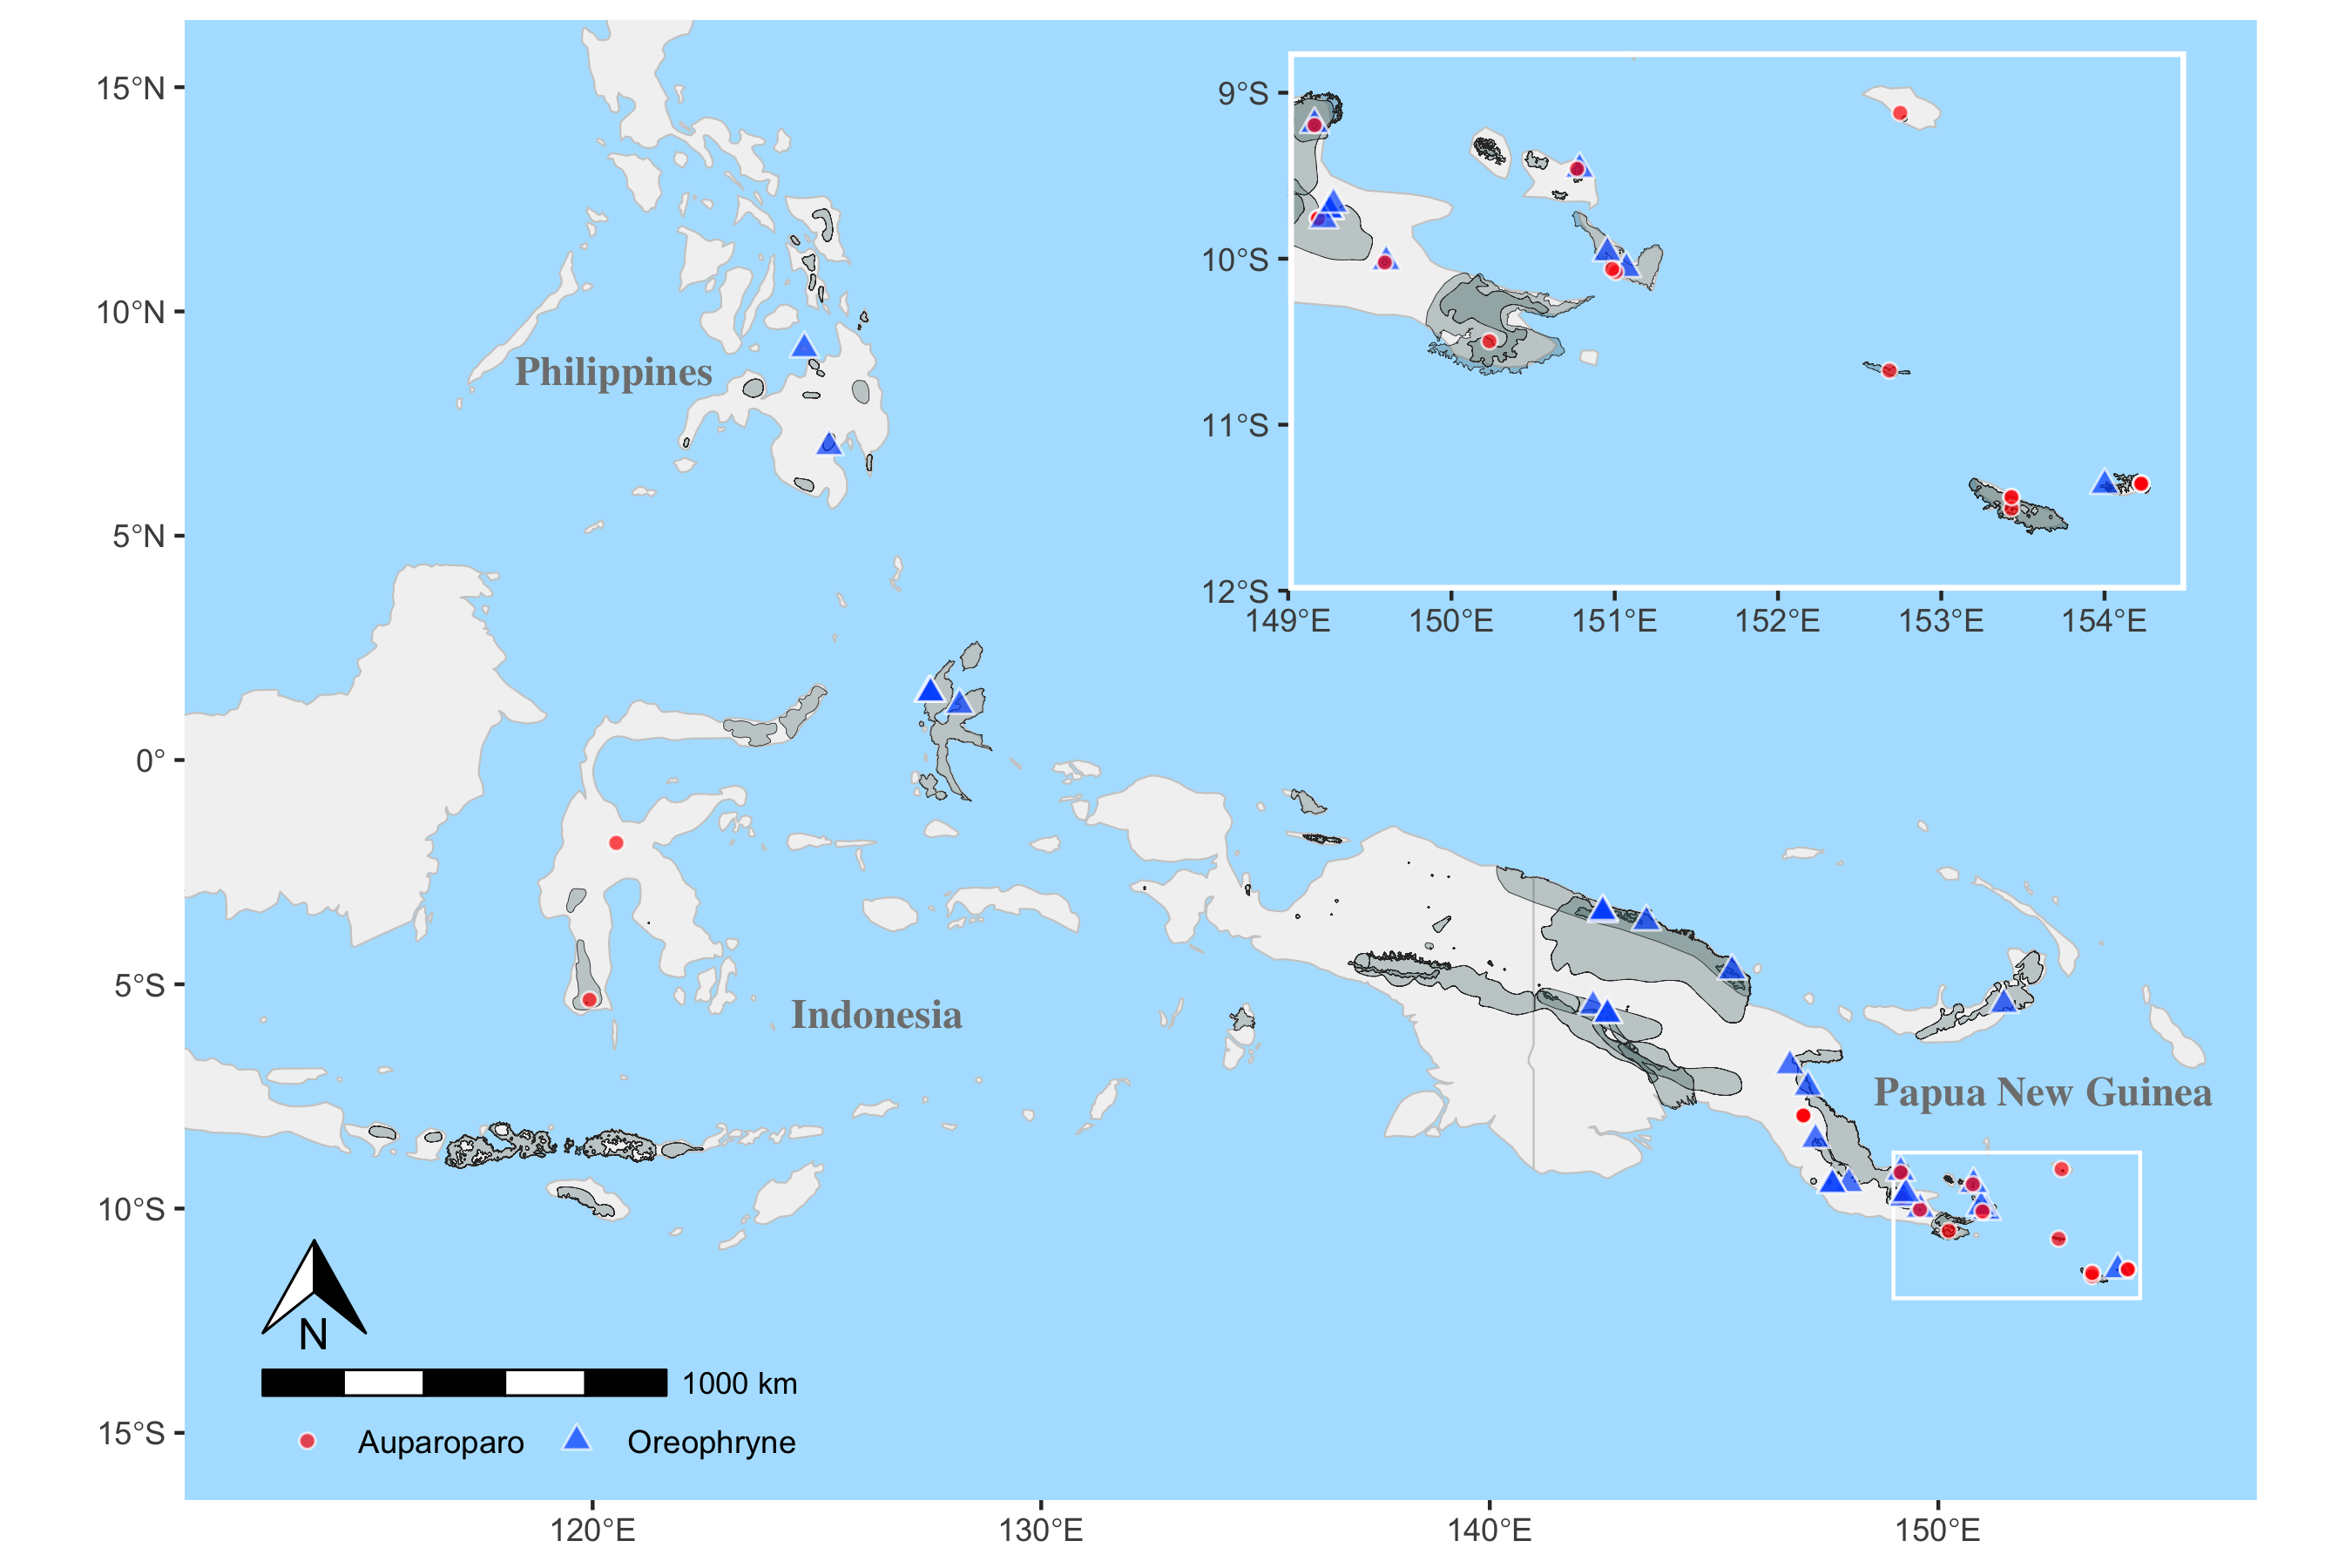
\includegraphics[width=1\linewidth,height=\textheight,keepaspectratio]{../Results/fig3.map-dot.png}

}

\caption{\label{fig-map}The known distribution of \emph{Oreophryne} as
currently recognized is plotted in grey polygons (data source IUCN,
2025), with points indicating \emph{Auparoparo} (red) and
\emph{Oreophryne} (blue) as assigned by our phylogenetic analysis
Figure~\ref{fig-phylo}. Note that there is range overlap along the East
Papuan Composite Terrane and on some offshore islands (see inset).}

\end{figure}%

\subsection{Taxonomy}\label{taxonomy}

We use a maximum crown-clade definitions for designating
\emph{Oreophryne} and \emph{Auparoparo} because the monophyly of these
taxa are strongly supported, and the relationships of these taxa to each
other and to other genera of Asterophryinae are well-supported (this
study, Hill \emph{et al.}, 2022, 2023b), as has been done for other
anuran taxa (Brown \emph{et al.}, 2015) following the methods of
phylogenetic nomenclature (De Queiroz \& Gauthier, 1990, 1992, 1994).
That is, we adopt phylogenetic definitions of these genera that
explicitly identify them as clades. Specifically, we define each genus
to include all descendants of the most recent common ancestor of the
type species and all other extant species that are more closely related
to it than to the type species of the other Asterophryine genera
recognized here. This definition is robust to uncertainty in basal
relationships such as in the case of adaptive radiations with short
branch lengths along the backbone as in Asterophryinae, as well as being
robust to identification of new species {[}{[}Find citation{]}{]}. We
retain the name \emph{Oreophryne} for species included in the
phylogenetic redefinition of \emph{Oreophryne}, and new clade name
\emph{Auparoparo} for newly designated species of \emph{Auparoparo}. The
previously defined polyphyletic \emph{Oreophryne} is indicated by
``sensu lato'', which contains many species which require molecular
phylogenetic assignment.

\textbf{Family \emph{Microhylidae} Günther 1858}\\
\textbf{Subfamily \emph{Asterophryinae} Günther 1858}\\
\textbf{Genus \emph{Oreophryne} Boettger 1895 amended}\\
\emph{Microhyla} Peters 1878\\
\emph{Callula} (Horst 1883) \emph{Oreophryne} Boettger 1895 Type
species: \emph{Oreophryne senckenbergiana} Boettger 1895. (=
\emph{Microhyla achatina} var. \emph{moluccensis} Peters 1878, by
monotypy) Placed on Official List of Generic Names in Zoology by Opinion
1266, Anonymous, 1984.\\
\emph{Sphenophryne} in part (Méhely 1897) \emph{Phrynixalus} (Stejneger
1908) \emph{Mehelyia} Wandolleck 1911, Type species: \emph{Meheylia
lineata} Wandolleck 1911 (=\emph{Sphenophryne biroi} Mehely 1897, by
subsequent designation of Parker 1934. Synonymy by Nieden (1926).\\
\emph{Cophixalus} in part (Boettger 1892)\\
\emph{Chaperina} in part (Taylor 1920)

\textbf{Diagnosis:} We note that there are no synapomorphies in adult
\emph{Oreophryne} that differ from the morphologically similar genus
\emph{Auparoparo}. Diagnoses should be made by molecular phylogenetic
analysis, based on the phylogenetic definition below. \emph{Oreophryne}
differs from most other genera in subfamily Asterophryinae, but not from
\emph{Auparoparo}, by the combination of (1) presence of highly reduced
clavicles (vs absence or elongate) which have a distinctly curved shape;
(2) presence of well developed digital pads, often with finger and toe
pads of similar size; (3) arboreal lifestyle (perch height
\textgreater2m above ground); (4) most species range in body size from
16mm (\emph{O. graminis}, Günther \& Richards, 2012) to 30mm, with a few
larger species \textasciitilde40mm (\emph{O. inornata}); (5) small to
invisible tympanum; (6) large eyes with horizontal pupils; (7)
occasional presence of toe webbing; (8) thin, elongated limbs; and (9)
in many species males that call with ``honk'' or ``peep'' types or in
some species ``rattle'' type. Some species of \emph{Oreophryne} may be
distinguished from \emph{Auparoparo} by roughly equal finger to toe pad
ratio and males calling with ``honk'' or ``peep'' but not ``whinny''
call types.

\textbf{Phylogenetic definition:} \emph{Oreophryne} Boettger 1895
(Converted Clade Name) is defined as the largest crown clade including
\emph{Oreophryne senckenbergiana} Boettger 1895 and excluding the type
species of the other genus-ranked clades listed in Table
Table~\ref{tbl-genus-types}.

\global\setlength{\Oldarrayrulewidth}{\arrayrulewidth}

\global\setlength{\Oldtabcolsep}{\tabcolsep}

\setlength{\tabcolsep}{2pt}

\renewcommand*{\arraystretch}{1.5}



\providecommand{\ascline}[3]{\noalign{\global\arrayrulewidth #1}\arrayrulecolor[HTML]{#2}\cline{#3}}

\begin{longtable}[c]{|p{1.40in}|p{6.27in}}

\caption{\label{tbl-genus-types}Genus-level clades of Asterophryinae and
their internal specifiers (type species or proxies).}

\tabularnewline

\ascline{1.5pt}{666666}{1-2}

\multicolumn{1}{>{\raggedright}m{\dimexpr 1.4in+0\tabcolsep}}{\advance\leftskip by 2.0pt\relax \advance\rightskip by 2.0pt\relax \textcolor[HTML]{666666}{\fontsize{11}{11}\selectfont{{\fontspec{Helvetica} Genus-level\ clade}}}} & \multicolumn{1}{>{\raggedright}m{\dimexpr 6.27in+0\tabcolsep}}{\advance\leftskip by 2.0pt\relax \advance\rightskip by 2.0pt\relax \textcolor[HTML]{666666}{\fontsize{11}{11}\selectfont{{\fontspec{Helvetica} Internal\ Specifier\ (Type\ Species\ or\ proxy)}}}} \\

\ascline{1.5pt}{666666}{1-2}\endfirsthead 

\ascline{1.5pt}{666666}{1-2}

\multicolumn{1}{>{\raggedright}m{\dimexpr 1.4in+0\tabcolsep}}{\advance\leftskip by 2.0pt\relax \advance\rightskip by 2.0pt\relax \textcolor[HTML]{666666}{\fontsize{11}{11}\selectfont{{\fontspec{Helvetica} Genus-level\ clade}}}} & \multicolumn{1}{>{\raggedright}m{\dimexpr 6.27in+0\tabcolsep}}{\advance\leftskip by 2.0pt\relax \advance\rightskip by 2.0pt\relax \textcolor[HTML]{666666}{\fontsize{11}{11}\selectfont{{\fontspec{Helvetica} Internal\ Specifier\ (Type\ Species\ or\ proxy)}}}} \\

\ascline{1.5pt}{666666}{1-2}\endhead



\multicolumn{2}{>{\raggedright}m{\dimexpr 7.66in+2\tabcolsep}}{\advance\leftskip by 2.0pt\relax \advance\rightskip by 2.0pt\relax \textcolor[HTML]{666666}{\fontsize{11}{11}\selectfont{{\fontspec{Helvetica} *We\ note\ that\ the\ monophyly\ of\ }}}\textcolor[HTML]{666666}{\fontsize{11}{11}\selectfont{{\fontspec{Helvetica} \textit{Austrochaperina,\ Liophryne,\ Oxydactyla}}}}\textcolor[HTML]{666666}{\fontsize{11}{11}\selectfont{{\fontspec{Helvetica} ,\ and\ }}}\textcolor[HTML]{666666}{\fontsize{11}{11}\selectfont{{\fontspec{Helvetica} \textit{Sphenophryne}}}}\textcolor[HTML]{666666}{\fontsize{11}{11}\selectfont{{\fontspec{Helvetica} \ (and\ reciprocal\ monophyly\ of\ }}}\textcolor[HTML]{666666}{\fontsize{11}{11}\selectfont{{\fontspec{Helvetica} \textit{Genyophryne}}}}\textcolor[HTML]{666666}{\fontsize{11}{11}\selectfont{{\fontspec{Helvetica} \ [}}}\textcolor[HTML]{666666}{\fontsize{11}{11}\selectfont{{\fontspec{Helvetica} \textit{Genyophryne\ thomsoni}}}}\textcolor[HTML]{666666}{\fontsize{11}{11}\selectfont{{\fontspec{Helvetica} \ Boulenger,\ 1890]\ with\ respect\ to\ }}}\textcolor[HTML]{666666}{\fontsize{11}{11}\selectfont{{\fontspec{Helvetica} \textit{Liophryne\ +\ Oxytactyla\ +\ Sphenophryne}}}}\textcolor[HTML]{666666}{\fontsize{11}{11}\selectfont{{\fontspec{Helvetica} )\ has\ not\ yet\ been\ established.\ }}}\textcolor[HTML]{666666}{\fontsize{11}{11}\selectfont{{\fontspec{Helvetica} \textit{Austrochaperina}}}}\textcolor[HTML]{666666}{\fontsize{11}{11}\selectfont{{\fontspec{Helvetica} \ is\ polyphyletic\ in\ recent\ phylogenies\ with\ possibly\ three\ monophyletic\ clades\ that\ are\ not\ sister\ taxa\ (Figure\ @fig-phylo).}}}} \\

\endlastfoot



\multicolumn{1}{>{\raggedright}m{\dimexpr 1.4in+0\tabcolsep}}{\advance\leftskip by 2.0pt\relax \advance\rightskip by 2.0pt\relax \textcolor[HTML]{666666}{\fontsize{11}{11}\selectfont{{\fontspec{Helvetica} \textit{Asterophrys}}}}} & \multicolumn{1}{>{\raggedright}m{\dimexpr 6.27in+0\tabcolsep}}{\advance\leftskip by 2.0pt\relax \advance\rightskip by 2.0pt\relax \textcolor[HTML]{666666}{\fontsize{11}{11}\selectfont{{\fontspec{Helvetica} \textit{\ Asterophrys\ turpicola}}}}\textcolor[HTML]{666666}{\fontsize{11}{11}\selectfont{{\fontspec{Helvetica} \ }}}\textcolor[HTML]{666666}{\fontsize{11}{11}\selectfont{{\fontspec{Helvetica} \ (Schlegel\ 1837)}}}} \\





\multicolumn{1}{>{\raggedright}m{\dimexpr 1.4in+0\tabcolsep}}{\advance\leftskip by 2.0pt\relax \advance\rightskip by 2.0pt\relax \textcolor[HTML]{666666}{\fontsize{11}{11}\selectfont{{\fontspec{Helvetica} \textit{Auparoparo}}}}} & \multicolumn{1}{>{\raggedright}m{\dimexpr 6.27in+0\tabcolsep}}{\advance\leftskip by 2.0pt\relax \advance\rightskip by 2.0pt\relax \textcolor[HTML]{666666}{\fontsize{11}{11}\selectfont{{\fontspec{Helvetica} \textit{\ Auparoparo\ penelopeia}}}}\textcolor[HTML]{666666}{\fontsize{11}{11}\selectfont{{\fontspec{Helvetica} \ }}}\textcolor[HTML]{666666}{\fontsize{11}{11}\selectfont{{\fontspec{Helvetica} \ (Kraus\ 2016)}}}} \\





\multicolumn{1}{>{\raggedright}m{\dimexpr 1.4in+0\tabcolsep}}{\advance\leftskip by 2.0pt\relax \advance\rightskip by 2.0pt\relax \textcolor[HTML]{666666}{\fontsize{11}{11}\selectfont{{\fontspec{Helvetica} \textit{Austrochaperina*}}}}} & \multicolumn{1}{>{\raggedright}m{\dimexpr 6.27in+0\tabcolsep}}{\advance\leftskip by 2.0pt\relax \advance\rightskip by 2.0pt\relax \textcolor[HTML]{666666}{\fontsize{11}{11}\selectfont{{\fontspec{Helvetica} \textit{\ Austrochaperina\ palmipes}}}}\textcolor[HTML]{666666}{\fontsize{11}{11}\selectfont{{\fontspec{Helvetica} \ }}}\textcolor[HTML]{666666}{\fontsize{11}{11}\selectfont{{\fontspec{Helvetica} \ (Zweifel\ 1956)}}}} \\





\multicolumn{1}{>{\raggedright}m{\dimexpr 1.4in+0\tabcolsep}}{\advance\leftskip by 2.0pt\relax \advance\rightskip by 2.0pt\relax \textcolor[HTML]{666666}{\fontsize{11}{11}\selectfont{{\fontspec{Helvetica} \textit{Austrochaperina*}}}}} & \multicolumn{1}{>{\raggedright}m{\dimexpr 6.27in+0\tabcolsep}}{\advance\leftskip by 2.0pt\relax \advance\rightskip by 2.0pt\relax \textcolor[HTML]{666666}{\fontsize{11}{11}\selectfont{{\fontspec{Helvetica} \textit{\ Austrochaperina\ robusta}}}}\textcolor[HTML]{666666}{\fontsize{11}{11}\selectfont{{\fontspec{Helvetica} \ }}}\textcolor[HTML]{666666}{\fontsize{11}{11}\selectfont{{\fontspec{Helvetica} \ Fry\ 1912}}}} \\





\multicolumn{1}{>{\raggedright}m{\dimexpr 1.4in+0\tabcolsep}}{\advance\leftskip by 2.0pt\relax \advance\rightskip by 2.0pt\relax \textcolor[HTML]{666666}{\fontsize{11}{11}\selectfont{{\fontspec{Helvetica} \textit{Barygenys}}}}} & \multicolumn{1}{>{\raggedright}m{\dimexpr 6.27in+0\tabcolsep}}{\advance\leftskip by 2.0pt\relax \advance\rightskip by 2.0pt\relax \textcolor[HTML]{666666}{\fontsize{11}{11}\selectfont{{\fontspec{Helvetica} \textit{\ Barygenys\ cheesmanae}}}}\textcolor[HTML]{666666}{\fontsize{11}{11}\selectfont{{\fontspec{Helvetica} \ }}}\textcolor[HTML]{666666}{\fontsize{11}{11}\selectfont{{\fontspec{Helvetica} \ Parker\ 1936}}}} \\





\multicolumn{1}{>{\raggedright}m{\dimexpr 1.4in+0\tabcolsep}}{\advance\leftskip by 2.0pt\relax \advance\rightskip by 2.0pt\relax \textcolor[HTML]{666666}{\fontsize{11}{11}\selectfont{{\fontspec{Helvetica} \textit{Callulops}}}}} & \multicolumn{1}{>{\raggedright}m{\dimexpr 6.27in+0\tabcolsep}}{\advance\leftskip by 2.0pt\relax \advance\rightskip by 2.0pt\relax \textcolor[HTML]{666666}{\fontsize{11}{11}\selectfont{{\fontspec{Helvetica} \textit{Callulops\ doriae}}}}\textcolor[HTML]{666666}{\fontsize{11}{11}\selectfont{{\fontspec{Helvetica} \ }}}\textcolor[HTML]{666666}{\fontsize{11}{11}\selectfont{{\fontspec{Helvetica} \ Boulenger\ 1888}}}} \\





\multicolumn{1}{>{\raggedright}m{\dimexpr 1.4in+0\tabcolsep}}{\advance\leftskip by 2.0pt\relax \advance\rightskip by 2.0pt\relax \textcolor[HTML]{666666}{\fontsize{11}{11}\selectfont{{\fontspec{Helvetica} \textit{Choerophryne}}}}} & \multicolumn{1}{>{\raggedright}m{\dimexpr 6.27in+0\tabcolsep}}{\advance\leftskip by 2.0pt\relax \advance\rightskip by 2.0pt\relax \textcolor[HTML]{666666}{\fontsize{11}{11}\selectfont{{\fontspec{Helvetica} \textit{\ Choerophryne\ proboscidea}}}}\textcolor[HTML]{666666}{\fontsize{11}{11}\selectfont{{\fontspec{Helvetica} \ }}}\textcolor[HTML]{666666}{\fontsize{11}{11}\selectfont{{\fontspec{Helvetica} \ Van\ Kampen\ 1914}}}} \\





\multicolumn{1}{>{\raggedright}m{\dimexpr 1.4in+0\tabcolsep}}{\advance\leftskip by 2.0pt\relax \advance\rightskip by 2.0pt\relax \textcolor[HTML]{666666}{\fontsize{11}{11}\selectfont{{\fontspec{Helvetica} \textit{Cophixalus}}}}} & \multicolumn{1}{>{\raggedright}m{\dimexpr 6.27in+0\tabcolsep}}{\advance\leftskip by 2.0pt\relax \advance\rightskip by 2.0pt\relax \textcolor[HTML]{666666}{\fontsize{11}{11}\selectfont{{\fontspec{Helvetica} \textit{\ Cophixalus\ verrucosus}}}}\textcolor[HTML]{666666}{\fontsize{11}{11}\selectfont{{\fontspec{Helvetica} \ }}}\textcolor[HTML]{666666}{\fontsize{11}{11}\selectfont{{\fontspec{Helvetica} \ (Boulenger,\ 1898)}}}} \\





\multicolumn{1}{>{\raggedright}m{\dimexpr 1.4in+0\tabcolsep}}{\advance\leftskip by 2.0pt\relax \advance\rightskip by 2.0pt\relax \textcolor[HTML]{666666}{\fontsize{11}{11}\selectfont{{\fontspec{Helvetica} \textit{Copiula}}}}} & \multicolumn{1}{>{\raggedright}m{\dimexpr 6.27in+0\tabcolsep}}{\advance\leftskip by 2.0pt\relax \advance\rightskip by 2.0pt\relax \textcolor[HTML]{666666}{\fontsize{11}{11}\selectfont{{\fontspec{Helvetica} \textit{\ Copiula\ oxyrhina}}}}\textcolor[HTML]{666666}{\fontsize{11}{11}\selectfont{{\fontspec{Helvetica} \ }}}\textcolor[HTML]{666666}{\fontsize{11}{11}\selectfont{{\fontspec{Helvetica} \ (Boulenger\ 1898)}}}} \\





\multicolumn{1}{>{\raggedright}m{\dimexpr 1.4in+0\tabcolsep}}{\advance\leftskip by 2.0pt\relax \advance\rightskip by 2.0pt\relax \textcolor[HTML]{666666}{\fontsize{11}{11}\selectfont{{\fontspec{Helvetica} \textit{Genyophryne*}}}}} & \multicolumn{1}{>{\raggedright}m{\dimexpr 6.27in+0\tabcolsep}}{\advance\leftskip by 2.0pt\relax \advance\rightskip by 2.0pt\relax \textcolor[HTML]{666666}{\fontsize{11}{11}\selectfont{{\fontspec{Helvetica} \textit{\ Genyophryne\ thomsoni}}}}\textcolor[HTML]{666666}{\fontsize{11}{11}\selectfont{{\fontspec{Helvetica} \ }}}\textcolor[HTML]{666666}{\fontsize{11}{11}\selectfont{{\fontspec{Helvetica} \ Boulenger,\ 1890}}}} \\





\multicolumn{1}{>{\raggedright}m{\dimexpr 1.4in+0\tabcolsep}}{\advance\leftskip by 2.0pt\relax \advance\rightskip by 2.0pt\relax \textcolor[HTML]{666666}{\fontsize{11}{11}\selectfont{{\fontspec{Helvetica} \textit{Hylophorbus}}}}} & \multicolumn{1}{>{\raggedright}m{\dimexpr 6.27in+0\tabcolsep}}{\advance\leftskip by 2.0pt\relax \advance\rightskip by 2.0pt\relax \textcolor[HTML]{666666}{\fontsize{11}{11}\selectfont{{\fontspec{Helvetica} \textit{\ Hylophorbus\ rufescens}}}}\textcolor[HTML]{666666}{\fontsize{11}{11}\selectfont{{\fontspec{Helvetica} \ }}}\textcolor[HTML]{666666}{\fontsize{11}{11}\selectfont{{\fontspec{Helvetica} \ Macleay\ 1878}}}} \\





\multicolumn{1}{>{\raggedright}m{\dimexpr 1.4in+0\tabcolsep}}{\advance\leftskip by 2.0pt\relax \advance\rightskip by 2.0pt\relax \textcolor[HTML]{666666}{\fontsize{11}{11}\selectfont{{\fontspec{Helvetica} \textit{Mantophyrne}}}}} & \multicolumn{1}{>{\raggedright}m{\dimexpr 6.27in+0\tabcolsep}}{\advance\leftskip by 2.0pt\relax \advance\rightskip by 2.0pt\relax \textcolor[HTML]{666666}{\fontsize{11}{11}\selectfont{{\fontspec{Helvetica} \textit{\ Mantophryne\ lateralis}}}}\textcolor[HTML]{666666}{\fontsize{11}{11}\selectfont{{\fontspec{Helvetica} \ }}}\textcolor[HTML]{666666}{\fontsize{11}{11}\selectfont{{\fontspec{Helvetica} \ Boulenger\ 1897}}}} \\





\multicolumn{1}{>{\raggedright}m{\dimexpr 1.4in+0\tabcolsep}}{\advance\leftskip by 2.0pt\relax \advance\rightskip by 2.0pt\relax \textcolor[HTML]{666666}{\fontsize{11}{11}\selectfont{{\fontspec{Helvetica} \textit{Liophryne*}}}}} & \multicolumn{1}{>{\raggedright}m{\dimexpr 6.27in+0\tabcolsep}}{\advance\leftskip by 2.0pt\relax \advance\rightskip by 2.0pt\relax \textcolor[HTML]{666666}{\fontsize{11}{11}\selectfont{{\fontspec{Helvetica} \textit{\ Liophryne\ rhododactyla}}}}\textcolor[HTML]{666666}{\fontsize{11}{11}\selectfont{{\fontspec{Helvetica} \ }}}\textcolor[HTML]{666666}{\fontsize{11}{11}\selectfont{{\fontspec{Helvetica} \ (Boulenger\ 1897)}}}} \\





\multicolumn{1}{>{\raggedright}m{\dimexpr 1.4in+0\tabcolsep}}{\advance\leftskip by 2.0pt\relax \advance\rightskip by 2.0pt\relax \textcolor[HTML]{666666}{\fontsize{11}{11}\selectfont{{\fontspec{Helvetica} \textit{Oreophryne}}}}} & \multicolumn{1}{>{\raggedright}m{\dimexpr 6.27in+0\tabcolsep}}{\advance\leftskip by 2.0pt\relax \advance\rightskip by 2.0pt\relax \textcolor[HTML]{666666}{\fontsize{11}{11}\selectfont{{\fontspec{Helvetica} \textit{\ Oreophryne\ senckenbergiana}}}}\textcolor[HTML]{666666}{\fontsize{11}{11}\selectfont{{\fontspec{Helvetica} \ }}}\textcolor[HTML]{666666}{\fontsize{11}{11}\selectfont{{\fontspec{Helvetica} \ Boettger\ 1895}}}\textcolor[HTML]{666666}{\fontsize{11}{11}\selectfont{{\fontspec{Helvetica} \ (=}}}\textcolor[HTML]{666666}{\fontsize{11}{11}\selectfont{{\fontspec{Helvetica} \textit{\ O.\ moluccensis}}}}\textcolor[HTML]{666666}{\fontsize{11}{11}\selectfont{{\fontspec{Helvetica} \ (Peters\ and\ Doria\ 1878)}}}\textcolor[HTML]{666666}{\fontsize{11}{11}\selectfont{{\fontspec{Helvetica} )}}}} \\





\multicolumn{1}{>{\raggedright}m{\dimexpr 1.4in+0\tabcolsep}}{\advance\leftskip by 2.0pt\relax \advance\rightskip by 2.0pt\relax \textcolor[HTML]{666666}{\fontsize{11}{11}\selectfont{{\fontspec{Helvetica} \textit{Oxydactyla}}}}} & \multicolumn{1}{>{\raggedright}m{\dimexpr 6.27in+0\tabcolsep}}{\advance\leftskip by 2.0pt\relax \advance\rightskip by 2.0pt\relax \textcolor[HTML]{666666}{\fontsize{11}{11}\selectfont{{\fontspec{Helvetica} \textit{\ Oxydactyla\ brevicrus}}}}\textcolor[HTML]{666666}{\fontsize{11}{11}\selectfont{{\fontspec{Helvetica} \ }}}\textcolor[HTML]{666666}{\fontsize{11}{11}\selectfont{{\fontspec{Helvetica} \ (Van\ Kampen\ 1913)}}}} \\





\multicolumn{1}{>{\raggedright}m{\dimexpr 1.4in+0\tabcolsep}}{\advance\leftskip by 2.0pt\relax \advance\rightskip by 2.0pt\relax \textcolor[HTML]{666666}{\fontsize{11}{11}\selectfont{{\fontspec{Helvetica} \textit{Paedophryne}}}}} & \multicolumn{1}{>{\raggedright}m{\dimexpr 6.27in+0\tabcolsep}}{\advance\leftskip by 2.0pt\relax \advance\rightskip by 2.0pt\relax \textcolor[HTML]{666666}{\fontsize{11}{11}\selectfont{{\fontspec{Helvetica} \textit{\ Paedophryne\ kathismaphlox}}}}\textcolor[HTML]{666666}{\fontsize{11}{11}\selectfont{{\fontspec{Helvetica} \ }}}\textcolor[HTML]{666666}{\fontsize{11}{11}\selectfont{{\fontspec{Helvetica} \ Kraus\ 2010}}}} \\





\multicolumn{1}{>{\raggedright}m{\dimexpr 1.4in+0\tabcolsep}}{\advance\leftskip by 2.0pt\relax \advance\rightskip by 2.0pt\relax \textcolor[HTML]{666666}{\fontsize{11}{11}\selectfont{{\fontspec{Helvetica} \textit{Sphenophryne*}}}}} & \multicolumn{1}{>{\raggedright}m{\dimexpr 6.27in+0\tabcolsep}}{\advance\leftskip by 2.0pt\relax \advance\rightskip by 2.0pt\relax \textcolor[HTML]{666666}{\fontsize{11}{11}\selectfont{{\fontspec{Helvetica} \textit{\ Sphenophryne\ cornuta}}}}\textcolor[HTML]{666666}{\fontsize{11}{11}\selectfont{{\fontspec{Helvetica} \ }}}\textcolor[HTML]{666666}{\fontsize{11}{11}\selectfont{{\fontspec{Helvetica} \ Peters\ and\ Doria\ 1878}}}} \\





\multicolumn{1}{>{\raggedright}m{\dimexpr 1.4in+0\tabcolsep}}{\advance\leftskip by 2.0pt\relax \advance\rightskip by 2.0pt\relax \textcolor[HTML]{666666}{\fontsize{11}{11}\selectfont{{\fontspec{Helvetica} \textit{Xenorhina}}}}} & \multicolumn{1}{>{\raggedright}m{\dimexpr 6.27in+0\tabcolsep}}{\advance\leftskip by 2.0pt\relax \advance\rightskip by 2.0pt\relax \textcolor[HTML]{666666}{\fontsize{11}{11}\selectfont{{\fontspec{Helvetica} \textit{\ Xenorhina\ oxycephala}}}}\textcolor[HTML]{666666}{\fontsize{11}{11}\selectfont{{\fontspec{Helvetica} \ }}}\textcolor[HTML]{666666}{\fontsize{11}{11}\selectfont{{\fontspec{Helvetica} \ (Schlegel\ 1858)}}}} \\

\ascline{1.5pt}{666666}{1-2}


\end{longtable}

\arrayrulecolor[HTML]{000000}

\global\setlength{\arrayrulewidth}{\Oldarrayrulewidth}

\global\setlength{\tabcolsep}{\Oldtabcolsep}

\renewcommand*{\arraystretch}{1}

\textbf{Composition:} Our results support the retention of 17 species in
\emph{Oreophryne} with molecular evidence (Table~\ref{tbl-transfers}):
\emph{Oreophryne anamiatoi} Kraus 2009, \emph{O. anulata} (Stejneger
1908), \emph{O. aurora} Kraus 2016, \emph{O. biroi} Mehely 1897,
\emph{O. brachypus} Werner 1898, \emph{O. cameroni} Kraus 2013, \emph{O.
geislerorum} Boettger 1892, \emph{O. graminis} Gunther 2012, \emph{O.
inornata} Zweifel 1956, \emph{O. lemur} Kraus 2016, \emph{O. loriae}
Boulenger 1898, \emph{O. nana} Brown 1967, \emph{O. notata} Zweifel
2003, \emph{O. parkeri} Loveridge 1955, \emph{O. parkopanorum} Kraus
2013, \emph{O. philosylleptoris} Kraus 2016, and \emph{O.
senckenbergiana} Boettger 1895. A number of species were not available
for our study but should molecular evidence demonstrate their
relationship within \emph{Oreophryne}, those species should also retain
their generic identity.

\textbf{Distribution:} The range of confirmed \emph{Oreophryne} species
in this dataset remains nearly as broad as previously defined
(Figure~\ref{fig-map}), from the Philippines and Indonesia to the
southeastern most tip of mainland New Guinea and several near-shore
islands (Fergusson, and Normanby Is.) and the distant Rossel Island of
the Louisiade Archipelago. However, the transfer of species which occupy
Woodlark Islands and Misima and Sudest Islands of the Louisaide
Archipelago reduces the known range of \emph{Oreophryne}. Woodlark
Island is inhabited by \emph{O. phoebe} {[}=\emph{Auparoparo phoebe}{]},
Misima Island is inhabited by \emph{O. picticrus} {[}=\emph{Auparoparo
picticrus}{]}, and Sudest Island is inhabited by \emph{O. ezra} and
\emph{O. meliades} {[}= \emph{Auparoparo ezra} and \emph{Auparoparo
meliades}{]}.

\textbf{Genus \emph{Auparoparo} gen. nov.}\\
\emph{Oreophryne} in part (Boettger, 1895)\\
\emph{Sphenophryne} in part (Boulenger, 1897)\\
Type species \emph{Oreophryne penelopeia} (Kraus, 2016)
{[}=\emph{Auparoparo penelopeia}{]}

\textbf{Diagnosis:} Currently, there are no known synapomorphies in
adult \emph{Auparoparo} that differ from the morphologically similar
genus \emph{Oreophryne}. Diagnoses should be made by molecular
phylogenetic analysis, based on the phylogenetic definition below.
\emph{Auparoparo} differs from most other genera in subfamily
Asterophryinae, but not from \emph{Oreophryne}, by the combination of
(1) presence of highly reduced clavicles (vs absence or elongate) which
have a distinctly curved shape; (2) presence of well developed digital
discs, with finger discs notably wider than toe discs (typically 20\% or
more); (3) arboreal lifestyle (perch height \textgreater2m above
ground); (4) small to moderately large body size in known species, from
16mm (\emph{A. brunnea} Kraus 2017) to 25 mm (\emph{A. picticrus} Kraus
2016); (5) small to invisible tympanum; (6) large eyes with horizontal
pupils; (7) occasional presence of toe webbing; (8) and thin, elongated
limbs; and (9) and in many species males that call with a ``whinny''
call type or in some species ``rattle'' type. Some species of
\emph{Auparoparo} may be distinguished from \emph{Oreophryne} by larger
finger pads than toe pads and males calling with ``whinny'' but not
``honk'' or ``peep'' call types.

\textbf{Phylogenetic definition:} \emph{Auparoparo} (New Clade Name)
applies to the largest crown clade including \emph{Auparoparo penelopia}
(Kraus 2016) and excluding the type species of the other genus-ranked
clades listed in Table~\ref{tbl-genus-types}.

\textbf{Composition:} We transfer eleven named species from
\emph{Oreophryne} into \emph{Auparoparo} (Table~\ref{tbl-transfers}):
\emph{Auparoparo brunnea} (Kraus, 2017), \emph{A. equus} (Kraus, 2016),
\emph{A. ezra} (Kraus \& Allison, 2009), \emph{A. insulana} (Zweifel,
1956), \emph{A. matawan} (Kraus, 2016), \emph{A. meliades} (Kraus,
2016), \emph{A. penelopeia} (Kraus, 2016), \emph{A. phoebe} (Kraus,
2017), \emph{A. picticrus} (Kraus, 2016), \emph{A. penelopia} (Kraus,
2016), \emph{A. variabilis} (Boulenger, 1896).

\textbf{Distribution:} Southeastern tip of mainland Papua New Guinea and
satellite islands (Fergusson, Misima, Normanby, Rossel, Sudest, Woodlark
Is.), Sulawesi.

\textbf{Etymology:} The generic name \emph{Auparoparo} comes from the
indigenous language, Motu, which is widely spoken in the region of Papua
New Guinea in which this genus is found. It is a combination of the
words ``au'' (tree) and ``paro paro'' (frog). Motu is not a gendered
language, however, for nomenclatural purposes we designate the genus
\emph{Auparoparo} as feminine, thereby preserving the gender of existing
species names.

\section{Discussion}\label{discussion}

Our phylogenetic results (Hill \emph{et al.}, 2022; 2023b, this study)
provide clarity on the classification of the problematic genus
\emph{Oreophryne} sensu lato. We confirm that \emph{Oreophryne} sensu
lato is polyphyletic and consists of two reciprocally monophyletic
clades that are not sister taxa (Figure~\ref{fig-phylo}). Here we
designate ``\emph{Oreophryne} A'' in Hill \emph{et al.} (2022) as the
genus \emph{Oreophryne} because it contains the type species
\emph{Oreophryne senckenbergiana} Boettger 1895 with high support.
\emph{Oreophryne} is the earliest diverged genus in subfamily
Asterophryinae originating approximately 18 MYA (Hill \emph{et al.},
2022), and is sister to a clade composed of all the other genera. The
second clade, ``\emph{Oreophryne} B'' in Hill \emph{et al.} (2022), is
highly supported as a separate, non-sister genus, which originated
approximately 16 MYA and contains no known species that are the types of
any previously proposed genera. Thus, we designate this genus as
\emph{Auparoparo}, a tribute to the Motu language of the indigenous
peoples of the region.

\subsection{The Difficulty with Cryptic Genera: Can we tell them
apart?}\label{the-difficulty-with-cryptic-genera-can-we-tell-them-apart}

Perhaps the greatest testament to the crypticism of \emph{Oreophryne}
vs.~\emph{Auparoparo} is that no taxonomist was able to distinguish that
they are separate clades, independently evolved, in the 130 years
between their discovery and the present classification {[}Boettger
(1895); this study{]}. These species are indeed morphologically very
similar (Figure~\ref{fig-photos}) and our results provide some clues as
to why \emph{Oreophryne} taxonomy has been so difficult. We found
morphological synapomorphies for neither \emph{Auparoparo} nor
\emph{Oreophryne}, and moreover, no morphological features that can
diagnose either clade.

The traditional basis for assigning species to \emph{Oreophryne} has
primarily relied on a signature pectoral anatomy (whether original or
revised diagnosis, Parker, 1934; Zweifel, 2003). Our phylogenetic
results clearly show that this trait appears more than once, in both
\emph{Oreophryne} and \emph{Auparaparo}, is either a symplesiomorphy
(shared ancestral character) or a result of convergent or parallel
evolution, and perhaps adaptive for arboreality. Thus, the pectoral
anatomy is not a reliable diagnostic character in differentiating
between \emph{Oreophryne} and \emph{Auparoparo}. In studies across a
wide diversity of anurans, Soliz, Abdala, \& Tulli (2025) found that
anatomical variation of the pectoral girdle corresponds with functional
and ecological lifestyle demands, whereas Engelkes \emph{et al.} (2020)
found strong phylogenetic influence in the shape of the pectoral girdle.
The pectoral girdle would be excellent for further study within
Asterophryinae, as there are high elevation terrestrial species of
\emph{Oreophryne} sensu lato that possess the same pectoral trait
(Zweifel \emph{et al.}, 2005), as well as a few arboreal species within
other genera (\emph{Cophixalus}, \emph{Asterophrys}, \emph{Xenorhina})
with unknown pectoral morphology.

We further rexamined additional characters previously used to diagnose
\emph{Oreophryne} as well as characters conventionally used to diagnose
species of frogs. We conclude that pectoral girdle connector type
(Parker, 1934) and relative lengths of the 3rd and 5th toe are
uninformative and the degree of toe webbing is variable. It was
previously suggested that species in \emph{Oreophryne} sensu lato could
be divided into two groups based on possessing a cartilaginous or
ligamentous connection between the procoracoid cartilages and the
scapula (Kraus, 2013), with roughly half possessing each type (Parker,
1934). However, we found that cartilaginous and ligamentous connectors
are common across both genera (Table~\ref{tbl-morph}); therefore, these
traits are not synapmorphies for neither \emph{Oreophryne} nor
\emph{Auparoparo} and do not indicate monophyly for these clades. Of
species with toe webbing, \emph{Oreophryne} tends to be described as
having ``well webbed'' toes compared to \emph{Auparoparo}'s ``basal''
webbing (Table~\ref{tbl-morph}). However, the presence of intra-specific
variability combined with subjectivity in judging relative landmarks
(e.g., ``reaching the penultimate tubercle'', ``webbed 1/3 length of 5th
toe'', etc.), makes this feature difficult to standardize for generic
diagnostic use. Many of the morphological traits proposed by Parker
(1934) and Zweifel (2003) may in fact be a result of homoplasy via
convergent lifestyle or parallel evolution, and while they may prove
useful for ecomorphological identification or species diagnoses in
combination with other traits, they are not informative for generic
diagnosis.

We found only two characters with potential for imperfectly
distinguishing the genera: relative digital pad size (Parker, 1934;
Zweifel, 1956), and call type (e.g., Kraus, 2016). The relative widths
of the digit pads differs between genera: \emph{Auparoparo} tends to
have visibly larger finger pads in comparison to toe pads, whereas in
\emph{Oreophryne} the finger and toe pads are roughly equal in size
(Figure~\ref{fig-photos}, bottom row), although there is some overlap in
finger to toe pad ratio (Table~\ref{tbl-morph}). In some cases,
\emph{Auparoparo}'s finger pads display T-shapes while the toes are
often rounder and narrower. Whether there is any performance advantage
in larger finger pads compared to toes is unknown. Furthermore, a
handful of high-elevation \emph{Oreophryne} species not included in our
phylogeny and yet to be diagnosed by molecular phylogenetic analysis
have evolved terrestrial or fossorial habits and possess smaller digital
pads compared to their presumed arboreal relatives (Zweifel \emph{et
al.}, 2005).

Call features are increasingly used for diagnosing species of
\emph{Oreophryne}, with advertisement call types commonly categorized as
rattle, honk, whinny, peeping, or clicking (Kraus, 2016). We found honk
or peep call types are only found in \emph{Oroephryne} species in our
sample, while whinny calls are only found in \emph{Auparoparo} species,
and rattle calls are found in both genera (Table~\ref{tbl-morph}). We
note that several authors described species of both genera, thus the
difference between genera cannot be attributed to the investigator.
However, more complete sampling may add further complexity. As far as we
are aware there has been no comprehensive acoustic analysis across
\emph{Oreophryne} sensu lato. More research is needed to explore call
diversity both between species and across genera to undertand call
evolution and whether there any features that are distinctive of genera.

\subsection{Geographic Distribution}\label{geographic-distribution-1}

Both \emph{Oreophryne} and \emph{Auparoparo} are geographically centered
in the mainland New Guinea. \emph{Oreophryne} extends southward to the
Louisiade Archipelago and northward to the South Philippine Islands
(Hill \emph{et al.}, 2023b). Addition of the type species
\emph{Oreophryne senkenbergiana} expands the known range eastward to
North Maluku, Indonesia (Figure~\ref{fig-map}).

The known distribution of \emph{Auparoparo} is mainly clustered in the
southeastern tip of mainland Papua New Guinea (in the East Papuan
Composite Terrane) and satellite islands with two species in Sulawesi,
Indonesia. This suggests the possiblity of of interesting plate
tectonics resulting in this biogeographic distribution. Exploration of
intermediate localities may result in as yet undescribed or undiscovered
species of \emph{Auparoparo}. The geographic range is sure to grow with
additional phylogenetic sampling. For example \emph{Oreophryne} (sensu
lato) \emph{chlorops} (Günther \emph{et al.}, 2023) is a very large (SVL
\textgreater{} 40mm) species recently discovered from mid-elevation
mountains of the birdʻs neck region of Western Papua with clearly
enlarged finger pads relative to toe pads. If confirmed as
\emph{Auparoparo}, it would significantly expand the range of
\emph{Auparoparo} across New Guinea Island.

We found geographic range overlap between \emph{Oreophryne} and
\emph{Auparoparo} at multiple localities: on the mainland along the Mt.
Dayman Foothills, at the Mt. Simpson Massif, Mt. Trafalgar, and on the
oceanic islands of Normanby and Fergusson (both nearshore islands), and
Rossel island (hundreds of kilometers offshore), which presents
interesting questions regarding biogeography as well as their ecological
relationships. For example, \emph{Oreophryne inornata} and
\emph{Auparoparo insulana} have been collected at the same site
(Goodenough Island) and even the same microhabitats (Zweifel, 1956). Do
these species occupy the same niche, and what is the temporal history of
each colonization? Are both genera also present in the nearby islands of
Normanby and Fergusson (all part of the D'Entrecasteaux Archipelago)?
Obtaining additional geographical samples for inclusion in phylogenetic
analysis should be a high priority to gain a more complete understanding
of the geographic distribution and evolutionary history of both
\emph{Oreophryne} and \emph{Auparoparo}.

\subsection{How to Avoid a Misleading
Classification}\label{how-to-avoid-a-misleading-classification}

We adopt an explicitly phylogenetic framework for the new taxonomy of
the genera \emph{Oreophryne} and \emph{Auparoparo}, and to our
knowledge, this is the first time that phylogenetic nomenclature has
been applied within the subfamily Asterophryinae. A phylogenetic
definition of genera is advantageous especially because Asterophryinae
is an adaptive radiation. While we are increasingly confident that at
least 16 genera are indeed monophyletic, nevertheless, very short branch
lengths separate many of the genera along the backbone {[}Hill \emph{et
al.} (2022); this study{]}. A maximum-crown-clade definition with
multiple external specifiers is robust to uncertainty (i.e.,
rearrangements of order) along the backbone. We define each genus as the
largest crown clade including the internal specifier species for the
clade (i.e., the type species of the genus) but not the internal
specifier species of other asterophryine genera. For long-studied groups
such as Asterophryinae, it may not be possible to obtain a genetic
sample for type species that were collected in the 1800ʻs and early
1900ʻs, as these locations may be uncertain and/or remote, it may be
necessary to use a genetic sample from another species of the genus as a
proxy for the type species. Nevertheless, is increasingly clear that for
\emph{Oreophryne} and \emph{Auparoparo}, a molecular phylogenetic
approach is required for final confirmation of taxonomy.

Furthermore, a phylogenetic definition provides guidance for robust
classification. Given the deep histories of the two genera, it is
imperative that molecular confirmation of a species to either
\emph{Oreophryne} or \emph{Auparoparo} include not only members of the
other clade, but also members of \emph{Cophixalus}, \emph{Paedophryne},
or other closely related genera to clearly resolve whether the sample
shares an MRCA more closely with \emph{Oreophryne} or \emph{Auparoaro}.
The ability to resolve the ``boundaries'' of each monophyletic genus
requires it. For example, a phylogenetic analysis with only
\emph{Oreophryne} sensu lato and outgroups to Asterophryinae will show
grouping of \emph{Oreophryne} and \emph{Auparoparo} species because of
the lack of intervening species assigned to other Asterophryinae genera,
particularly \emph{Cophixalus} and \emph{Paedophryne}. An additional
difficulty here is that within \emph{Oreophryne} and \emph{Auparoparo},
there are subclades with deep histories (Hill \emph{et al.}, 2023a), so
care must be taken to ensure correct assignment to genus.

This study furthermore highlights the importance of taxonomic sampling
for robust phylogenetic results. Developing an orderly taxonomy in a
clade with over 350 named species (with perhaps as much as 40\% of
species in museum collections that are yet to be described, A. Allison,
unpublished) would be that much more challenging without the benefit of
generic diagnoses that follow evolutionary history.

\subsection{Why the Names Matter}\label{why-the-names-matter}

Clarifying the generic structure also facilitates appreciation for the
patterns of diversification within Asterophryinae. The evolutionary
history of this subfamily is characterized by several interesting trends
across genera: 1) a burst of ecological and species diversification
leading to generic-level clades occurring early in the history of the
subfamily (Hill \emph{et al.}, 2022), 2) a tendency toward niche
conservatism within genera, and 3) simultaneous dispersal of multiple
genera to offshore islands (Hill \emph{et al.}, 2022, 2023a) revealing
the very strong influence of plate tectonics for explaining the
historical dispersal patterns of this group. Finally, without distinct
generic names for the two clades represented by \emph{Oreophyne} and
\emph{Auparoparo}, it becomes much more difficult to appreciate
independently evolutionary histories embodied by each clade, that
aboreality has evolved at least twice in subfamily Asterophyrinae, and
would make it very difficult to appreciate the impressive paralleism
embodied by these speciose and successful genera. An accurate and
informative taxonomy serves to advance our understanding of Papuan
microhylids and their very interesting evolutionary history leading to
further discovery.

Lastly, we emphasize that future naming of species, genera, and higher
taxa should seek to recognize the language of the indigenous stewards of
the land and ecosystem from which they were discovered (Gillman \&
Wright, 2020). This is especially true of Asterophryinae frogs, whose
awe-inspiring diversity mirrors the rich cultural beauty and historical
complexity of Papuan people.

\section{Acknowledgements}\label{acknowledgements}

We thank Ben Evans and Iqbal Setiadi for generously providing samples
critical for this study, and Ethan Hill for his guidance and training on
the molecular and bioinformatics work. We are grateful to Molly Hagemann
for her excellent assistance in accessing Bishop Museum Vertebrate
Zoology Collections and data. We thank Neal Evenhuis for sharing expert
knowledge on type species, and Brianna Correa and Alexis Shulga for
providing comments which improved the manuscript. This is publication
234 from the School of Life Sciences, University of Hawaiʻi at Mānoa.

\section{Funding}\label{funding}

This study was made possible by a grant from the National Science
Foundation awarded to MB (DEB-1145733). We gratefully acknowledge
support from the School of Life Sciences, University of Hawai'i at M
̄anoa. University of Hawaii Information Technology Services --
Cyberinfrastructure resources were funded in part by a National Science
Foundation Major Research Instrumentation award (CNS-1920304).

\section{Data Availability}\label{data-availability}

The data underlying this article are available in the GenBank Nucleotide
Database{]} at \url{https://www.ncbi.nlm.nih.gov/genbank/} , and can be
accessed with {[}will be provided upon publication{]}. The codes and
datafiles needed to reproduce these results can be found at {[}GitHub
repository{]} with DOI {[}supplied upon publication{]}.

\section{Supplementary Table}\label{supplementary-table}

\global\setlength{\Oldarrayrulewidth}{\arrayrulewidth}

\global\setlength{\Oldtabcolsep}{\tabcolsep}

\setlength{\tabcolsep}{2pt}

\renewcommand*{\arraystretch}{1.5}



\providecommand{\ascline}[3]{\noalign{\global\arrayrulewidth #1}\arrayrulecolor[HTML]{#2}\cline{#3}}

\begin{longtable}[c]{|p{2.67in}|p{3.84in}|p{0.98in}|p{1.12in}|p{1.39in}|p{1.97in}}

\caption{\label{tbl-transfers}Classification of \emph{Auparoparo} and
\emph{Oreophryne} based on phylogenetic evidence from two mitochondrial
gene fragments (CytB, ND4) and three nuclear loci (BDNF, SIA, NXC).
Incertae sedis taxa require phylogenetic evidence for classification.}

\tabularnewline

\ascline{1.5pt}{666666}{1-6}

\multicolumn{1}{>{\raggedright}m{\dimexpr 2.67in+0\tabcolsep}}{\advance\leftskip by 2.0pt\relax \advance\rightskip by 2.0pt\relax \textcolor[HTML]{666666}{\fontsize{11}{11}\selectfont{{\fontspec{Helvetica} Original\ designation}}}} & \multicolumn{1}{>{\raggedright}m{\dimexpr 3.84in+0\tabcolsep}}{\advance\leftskip by 2.0pt\relax \advance\rightskip by 2.0pt\relax \textcolor[HTML]{666666}{\fontsize{11}{11}\selectfont{{\fontspec{Helvetica} Citation}}}} & \multicolumn{1}{>{\raggedright}m{\dimexpr 0.98in+0\tabcolsep}}{\advance\leftskip by 2.0pt\relax \advance\rightskip by 2.0pt\relax \textcolor[HTML]{666666}{\fontsize{11}{11}\selectfont{{\fontspec{Helvetica} Previous\ generic\ placement}}}} & \multicolumn{1}{>{\raggedright}m{\dimexpr 1.12in+0\tabcolsep}}{\advance\leftskip by 2.0pt\relax \advance\rightskip by 2.0pt\relax \textcolor[HTML]{666666}{\fontsize{11}{11}\selectfont{{\fontspec{Helvetica} Current\ generic\ placement}}}} & \multicolumn{1}{>{\raggedright}m{\dimexpr 1.39in+0\tabcolsep}}{\advance\leftskip by 2.0pt\relax \advance\rightskip by 2.0pt\relax \textcolor[HTML]{666666}{\fontsize{11}{11}\selectfont{{\fontspec{Helvetica} Species}}}} & \multicolumn{1}{>{\raggedright}m{\dimexpr 1.97in+0\tabcolsep}}{\advance\leftskip by 2.0pt\relax \advance\rightskip by 2.0pt\relax \textcolor[HTML]{666666}{\fontsize{11}{11}\selectfont{{\fontspec{Helvetica} Notes}}}} \\

\ascline{1.5pt}{666666}{1-6}\endfirsthead 

\ascline{1.5pt}{666666}{1-6}

\multicolumn{1}{>{\raggedright}m{\dimexpr 2.67in+0\tabcolsep}}{\advance\leftskip by 2.0pt\relax \advance\rightskip by 2.0pt\relax \textcolor[HTML]{666666}{\fontsize{11}{11}\selectfont{{\fontspec{Helvetica} Original\ designation}}}} & \multicolumn{1}{>{\raggedright}m{\dimexpr 3.84in+0\tabcolsep}}{\advance\leftskip by 2.0pt\relax \advance\rightskip by 2.0pt\relax \textcolor[HTML]{666666}{\fontsize{11}{11}\selectfont{{\fontspec{Helvetica} Citation}}}} & \multicolumn{1}{>{\raggedright}m{\dimexpr 0.98in+0\tabcolsep}}{\advance\leftskip by 2.0pt\relax \advance\rightskip by 2.0pt\relax \textcolor[HTML]{666666}{\fontsize{11}{11}\selectfont{{\fontspec{Helvetica} Previous\ generic\ placement}}}} & \multicolumn{1}{>{\raggedright}m{\dimexpr 1.12in+0\tabcolsep}}{\advance\leftskip by 2.0pt\relax \advance\rightskip by 2.0pt\relax \textcolor[HTML]{666666}{\fontsize{11}{11}\selectfont{{\fontspec{Helvetica} Current\ generic\ placement}}}} & \multicolumn{1}{>{\raggedright}m{\dimexpr 1.39in+0\tabcolsep}}{\advance\leftskip by 2.0pt\relax \advance\rightskip by 2.0pt\relax \textcolor[HTML]{666666}{\fontsize{11}{11}\selectfont{{\fontspec{Helvetica} Species}}}} & \multicolumn{1}{>{\raggedright}m{\dimexpr 1.97in+0\tabcolsep}}{\advance\leftskip by 2.0pt\relax \advance\rightskip by 2.0pt\relax \textcolor[HTML]{666666}{\fontsize{11}{11}\selectfont{{\fontspec{Helvetica} Notes}}}} \\

\ascline{1.5pt}{666666}{1-6}\endhead



\multicolumn{1}{>{\raggedright}m{\dimexpr 2.67in+0\tabcolsep}}{\advance\leftskip by 2.0pt\relax \advance\rightskip by 2.0pt\relax \textcolor[HTML]{666666}{\fontsize{11}{11}\selectfont{{\fontspec{Helvetica} \textit{Oreophryne\ anamiatoi\ }}}}} & \multicolumn{1}{>{\raggedright}m{\dimexpr 3.84in+0\tabcolsep}}{\advance\leftskip by 2.0pt\relax \advance\rightskip by 2.0pt\relax \textcolor[HTML]{666666}{\fontsize{11}{11}\selectfont{{\fontspec{Helvetica} (Kraus\ \&\ Allison,\ 2009)}}}} & \multicolumn{1}{>{\raggedright}m{\dimexpr 0.98in+0\tabcolsep}}{\advance\leftskip by 2.0pt\relax \advance\rightskip by 2.0pt\relax \textcolor[HTML]{666666}{\fontsize{11}{11}\selectfont{{\fontspec{Helvetica} \textit{Oreophryne}}}}} & \multicolumn{1}{>{\raggedright}m{\dimexpr 1.12in+0\tabcolsep}}{\advance\leftskip by 2.0pt\relax \advance\rightskip by 2.0pt\relax \textcolor[HTML]{666666}{\fontsize{11}{11}\selectfont{{\fontspec{Helvetica} \textit{Oreophryne}}}}} & \multicolumn{1}{>{\raggedright}m{\dimexpr 1.39in+0\tabcolsep}}{\advance\leftskip by 2.0pt\relax \advance\rightskip by 2.0pt\relax \textcolor[HTML]{666666}{\fontsize{11}{11}\selectfont{{\fontspec{Helvetica} \textit{anamiatoi}}}}} & \multicolumn{1}{>{\raggedright}m{\dimexpr 1.97in+0\tabcolsep}}{\advance\leftskip by 2.0pt\relax \advance\rightskip by 2.0pt\relax \textcolor[HTML]{666666}{\fontsize{11}{11}\selectfont{{\fontspec{Helvetica} Retained\ in\ Oreophryne}}}} \\





\multicolumn{1}{>{\raggedright}m{\dimexpr 2.67in+0\tabcolsep}}{\advance\leftskip by 2.0pt\relax \advance\rightskip by 2.0pt\relax \textcolor[HTML]{666666}{\fontsize{11}{11}\selectfont{{\fontspec{Helvetica} \textit{Phrynixalus\ anulatus\ }}}}} & \multicolumn{1}{>{\raggedright}m{\dimexpr 3.84in+0\tabcolsep}}{\advance\leftskip by 2.0pt\relax \advance\rightskip by 2.0pt\relax \textcolor[HTML]{666666}{\fontsize{11}{11}\selectfont{{\fontspec{Helvetica} (Stejneger,\ 1908)}}}} & \multicolumn{1}{>{\raggedright}m{\dimexpr 0.98in+0\tabcolsep}}{\advance\leftskip by 2.0pt\relax \advance\rightskip by 2.0pt\relax \textcolor[HTML]{666666}{\fontsize{11}{11}\selectfont{{\fontspec{Helvetica} \textit{Oreophryne}}}}} & \multicolumn{1}{>{\raggedright}m{\dimexpr 1.12in+0\tabcolsep}}{\advance\leftskip by 2.0pt\relax \advance\rightskip by 2.0pt\relax \textcolor[HTML]{666666}{\fontsize{11}{11}\selectfont{{\fontspec{Helvetica} \textit{Oreophryne}}}}} & \multicolumn{1}{>{\raggedright}m{\dimexpr 1.39in+0\tabcolsep}}{\advance\leftskip by 2.0pt\relax \advance\rightskip by 2.0pt\relax \textcolor[HTML]{666666}{\fontsize{11}{11}\selectfont{{\fontspec{Helvetica} \textit{anulata}}}}} & \multicolumn{1}{>{\raggedright}m{\dimexpr 1.97in+0\tabcolsep}}{\advance\leftskip by 2.0pt\relax \advance\rightskip by 2.0pt\relax \textcolor[HTML]{666666}{\fontsize{11}{11}\selectfont{{\fontspec{Helvetica} Retained\ in\ Oreophryne}}}} \\





\multicolumn{1}{>{\raggedright}m{\dimexpr 2.67in+0\tabcolsep}}{\advance\leftskip by 2.0pt\relax \advance\rightskip by 2.0pt\relax \textcolor[HTML]{666666}{\fontsize{11}{11}\selectfont{{\fontspec{Helvetica} \textit{Oreophryne\ aurora\ }}}}} & \multicolumn{1}{>{\raggedright}m{\dimexpr 3.84in+0\tabcolsep}}{\advance\leftskip by 2.0pt\relax \advance\rightskip by 2.0pt\relax \textcolor[HTML]{666666}{\fontsize{11}{11}\selectfont{{\fontspec{Helvetica} (Kraus,\ 2016)}}}} & \multicolumn{1}{>{\raggedright}m{\dimexpr 0.98in+0\tabcolsep}}{\advance\leftskip by 2.0pt\relax \advance\rightskip by 2.0pt\relax \textcolor[HTML]{666666}{\fontsize{11}{11}\selectfont{{\fontspec{Helvetica} \textit{Oreophryne}}}}} & \multicolumn{1}{>{\raggedright}m{\dimexpr 1.12in+0\tabcolsep}}{\advance\leftskip by 2.0pt\relax \advance\rightskip by 2.0pt\relax \textcolor[HTML]{666666}{\fontsize{11}{11}\selectfont{{\fontspec{Helvetica} \textit{Oreophryne}}}}} & \multicolumn{1}{>{\raggedright}m{\dimexpr 1.39in+0\tabcolsep}}{\advance\leftskip by 2.0pt\relax \advance\rightskip by 2.0pt\relax \textcolor[HTML]{666666}{\fontsize{11}{11}\selectfont{{\fontspec{Helvetica} \textit{aurora}}}}} & \multicolumn{1}{>{\raggedright}m{\dimexpr 1.97in+0\tabcolsep}}{\advance\leftskip by 2.0pt\relax \advance\rightskip by 2.0pt\relax \textcolor[HTML]{666666}{\fontsize{11}{11}\selectfont{{\fontspec{Helvetica} Retained\ in\ Oreophryne}}}} \\





\multicolumn{1}{>{\raggedright}m{\dimexpr 2.67in+0\tabcolsep}}{\advance\leftskip by 2.0pt\relax \advance\rightskip by 2.0pt\relax \textcolor[HTML]{666666}{\fontsize{11}{11}\selectfont{{\fontspec{Helvetica} \textit{Sphenophryne\ biroi\ }}}}} & \multicolumn{1}{>{\raggedright}m{\dimexpr 3.84in+0\tabcolsep}}{\advance\leftskip by 2.0pt\relax \advance\rightskip by 2.0pt\relax \textcolor[HTML]{666666}{\fontsize{11}{11}\selectfont{{\fontspec{Helvetica} (Méhely,\ 1897)}}}} & \multicolumn{1}{>{\raggedright}m{\dimexpr 0.98in+0\tabcolsep}}{\advance\leftskip by 2.0pt\relax \advance\rightskip by 2.0pt\relax \textcolor[HTML]{666666}{\fontsize{11}{11}\selectfont{{\fontspec{Helvetica} \textit{Oreophryne}}}}} & \multicolumn{1}{>{\raggedright}m{\dimexpr 1.12in+0\tabcolsep}}{\advance\leftskip by 2.0pt\relax \advance\rightskip by 2.0pt\relax \textcolor[HTML]{666666}{\fontsize{11}{11}\selectfont{{\fontspec{Helvetica} \textit{Oreophryne}}}}} & \multicolumn{1}{>{\raggedright}m{\dimexpr 1.39in+0\tabcolsep}}{\advance\leftskip by 2.0pt\relax \advance\rightskip by 2.0pt\relax \textcolor[HTML]{666666}{\fontsize{11}{11}\selectfont{{\fontspec{Helvetica} \textit{biroi}}}}} & \multicolumn{1}{>{\raggedright}m{\dimexpr 1.97in+0\tabcolsep}}{\advance\leftskip by 2.0pt\relax \advance\rightskip by 2.0pt\relax \textcolor[HTML]{666666}{\fontsize{11}{11}\selectfont{{\fontspec{Helvetica} Retained\ in\ Oreophryne}}}} \\





\multicolumn{1}{>{\raggedright}m{\dimexpr 2.67in+0\tabcolsep}}{\advance\leftskip by 2.0pt\relax \advance\rightskip by 2.0pt\relax \textcolor[HTML]{666666}{\fontsize{11}{11}\selectfont{{\fontspec{Helvetica} \textit{Hylella\ brachypus\ }}}}} & \multicolumn{1}{>{\raggedright}m{\dimexpr 3.84in+0\tabcolsep}}{\advance\leftskip by 2.0pt\relax \advance\rightskip by 2.0pt\relax \textcolor[HTML]{666666}{\fontsize{11}{11}\selectfont{{\fontspec{Helvetica} (Werner,\ 1898)}}}} & \multicolumn{1}{>{\raggedright}m{\dimexpr 0.98in+0\tabcolsep}}{\advance\leftskip by 2.0pt\relax \advance\rightskip by 2.0pt\relax \textcolor[HTML]{666666}{\fontsize{11}{11}\selectfont{{\fontspec{Helvetica} \textit{Oreophryne}}}}} & \multicolumn{1}{>{\raggedright}m{\dimexpr 1.12in+0\tabcolsep}}{\advance\leftskip by 2.0pt\relax \advance\rightskip by 2.0pt\relax \textcolor[HTML]{666666}{\fontsize{11}{11}\selectfont{{\fontspec{Helvetica} \textit{Oreophryne}}}}} & \multicolumn{1}{>{\raggedright}m{\dimexpr 1.39in+0\tabcolsep}}{\advance\leftskip by 2.0pt\relax \advance\rightskip by 2.0pt\relax \textcolor[HTML]{666666}{\fontsize{11}{11}\selectfont{{\fontspec{Helvetica} \textit{brachypus}}}}} & \multicolumn{1}{>{\raggedright}m{\dimexpr 1.97in+0\tabcolsep}}{\advance\leftskip by 2.0pt\relax \advance\rightskip by 2.0pt\relax \textcolor[HTML]{666666}{\fontsize{11}{11}\selectfont{{\fontspec{Helvetica} Retained\ in\ Oreophryne}}}} \\





\multicolumn{1}{>{\raggedright}m{\dimexpr 2.67in+0\tabcolsep}}{\advance\leftskip by 2.0pt\relax \advance\rightskip by 2.0pt\relax \textcolor[HTML]{666666}{\fontsize{11}{11}\selectfont{{\fontspec{Helvetica} \textit{Oreophryne\ cameroni\ }}}}} & \multicolumn{1}{>{\raggedright}m{\dimexpr 3.84in+0\tabcolsep}}{\advance\leftskip by 2.0pt\relax \advance\rightskip by 2.0pt\relax \textcolor[HTML]{666666}{\fontsize{11}{11}\selectfont{{\fontspec{Helvetica} (Kraus,\ 2013)}}}} & \multicolumn{1}{>{\raggedright}m{\dimexpr 0.98in+0\tabcolsep}}{\advance\leftskip by 2.0pt\relax \advance\rightskip by 2.0pt\relax \textcolor[HTML]{666666}{\fontsize{11}{11}\selectfont{{\fontspec{Helvetica} \textit{Oreophryne}}}}} & \multicolumn{1}{>{\raggedright}m{\dimexpr 1.12in+0\tabcolsep}}{\advance\leftskip by 2.0pt\relax \advance\rightskip by 2.0pt\relax \textcolor[HTML]{666666}{\fontsize{11}{11}\selectfont{{\fontspec{Helvetica} \textit{Oreophryne}}}}} & \multicolumn{1}{>{\raggedright}m{\dimexpr 1.39in+0\tabcolsep}}{\advance\leftskip by 2.0pt\relax \advance\rightskip by 2.0pt\relax \textcolor[HTML]{666666}{\fontsize{11}{11}\selectfont{{\fontspec{Helvetica} \textit{cameroni}}}}} & \multicolumn{1}{>{\raggedright}m{\dimexpr 1.97in+0\tabcolsep}}{\advance\leftskip by 2.0pt\relax \advance\rightskip by 2.0pt\relax \textcolor[HTML]{666666}{\fontsize{11}{11}\selectfont{{\fontspec{Helvetica} Retained\ in\ Oreophryne}}}} \\





\multicolumn{1}{>{\raggedright}m{\dimexpr 2.67in+0\tabcolsep}}{\advance\leftskip by 2.0pt\relax \advance\rightskip by 2.0pt\relax \textcolor[HTML]{666666}{\fontsize{11}{11}\selectfont{{\fontspec{Helvetica} \textit{Cophixalus\ geislerorum\ }}}}} & \multicolumn{1}{>{\raggedright}m{\dimexpr 3.84in+0\tabcolsep}}{\advance\leftskip by 2.0pt\relax \advance\rightskip by 2.0pt\relax \textcolor[HTML]{666666}{\fontsize{11}{11}\selectfont{{\fontspec{Helvetica} (Boettger,\ 1892)}}}} & \multicolumn{1}{>{\raggedright}m{\dimexpr 0.98in+0\tabcolsep}}{\advance\leftskip by 2.0pt\relax \advance\rightskip by 2.0pt\relax \textcolor[HTML]{666666}{\fontsize{11}{11}\selectfont{{\fontspec{Helvetica} \textit{Oreophryne}}}}} & \multicolumn{1}{>{\raggedright}m{\dimexpr 1.12in+0\tabcolsep}}{\advance\leftskip by 2.0pt\relax \advance\rightskip by 2.0pt\relax \textcolor[HTML]{666666}{\fontsize{11}{11}\selectfont{{\fontspec{Helvetica} \textit{Oreophryne}}}}} & \multicolumn{1}{>{\raggedright}m{\dimexpr 1.39in+0\tabcolsep}}{\advance\leftskip by 2.0pt\relax \advance\rightskip by 2.0pt\relax \textcolor[HTML]{666666}{\fontsize{11}{11}\selectfont{{\fontspec{Helvetica} \textit{geislerorum}}}}} & \multicolumn{1}{>{\raggedright}m{\dimexpr 1.97in+0\tabcolsep}}{\advance\leftskip by 2.0pt\relax \advance\rightskip by 2.0pt\relax \textcolor[HTML]{666666}{\fontsize{11}{11}\selectfont{{\fontspec{Helvetica} Retained\ in\ Oreophryne}}}} \\





\multicolumn{1}{>{\raggedright}m{\dimexpr 2.67in+0\tabcolsep}}{\advance\leftskip by 2.0pt\relax \advance\rightskip by 2.0pt\relax \textcolor[HTML]{666666}{\fontsize{11}{11}\selectfont{{\fontspec{Helvetica} \textit{Oreophryne\ graminis\ }}}}} & \multicolumn{1}{>{\raggedright}m{\dimexpr 3.84in+0\tabcolsep}}{\advance\leftskip by 2.0pt\relax \advance\rightskip by 2.0pt\relax \textcolor[HTML]{666666}{\fontsize{11}{11}\selectfont{{\fontspec{Helvetica} (Günther\ \&\ Richards,\ 2012)}}}} & \multicolumn{1}{>{\raggedright}m{\dimexpr 0.98in+0\tabcolsep}}{\advance\leftskip by 2.0pt\relax \advance\rightskip by 2.0pt\relax \textcolor[HTML]{666666}{\fontsize{11}{11}\selectfont{{\fontspec{Helvetica} \textit{Oreophryne}}}}} & \multicolumn{1}{>{\raggedright}m{\dimexpr 1.12in+0\tabcolsep}}{\advance\leftskip by 2.0pt\relax \advance\rightskip by 2.0pt\relax \textcolor[HTML]{666666}{\fontsize{11}{11}\selectfont{{\fontspec{Helvetica} \textit{Oreophryne}}}}} & \multicolumn{1}{>{\raggedright}m{\dimexpr 1.39in+0\tabcolsep}}{\advance\leftskip by 2.0pt\relax \advance\rightskip by 2.0pt\relax \textcolor[HTML]{666666}{\fontsize{11}{11}\selectfont{{\fontspec{Helvetica} \textit{graminis}}}}} & \multicolumn{1}{>{\raggedright}m{\dimexpr 1.97in+0\tabcolsep}}{\advance\leftskip by 2.0pt\relax \advance\rightskip by 2.0pt\relax \textcolor[HTML]{666666}{\fontsize{11}{11}\selectfont{{\fontspec{Helvetica} Retained\ in\ Oreophryne}}}} \\





\multicolumn{1}{>{\raggedright}m{\dimexpr 2.67in+0\tabcolsep}}{\advance\leftskip by 2.0pt\relax \advance\rightskip by 2.0pt\relax \textcolor[HTML]{666666}{\fontsize{11}{11}\selectfont{{\fontspec{Helvetica} \textit{Oreophryne\ inornata\ }}}}} & \multicolumn{1}{>{\raggedright}m{\dimexpr 3.84in+0\tabcolsep}}{\advance\leftskip by 2.0pt\relax \advance\rightskip by 2.0pt\relax \textcolor[HTML]{666666}{\fontsize{11}{11}\selectfont{{\fontspec{Helvetica} (Zweifel,\ 1956)}}}} & \multicolumn{1}{>{\raggedright}m{\dimexpr 0.98in+0\tabcolsep}}{\advance\leftskip by 2.0pt\relax \advance\rightskip by 2.0pt\relax \textcolor[HTML]{666666}{\fontsize{11}{11}\selectfont{{\fontspec{Helvetica} \textit{Oreophryne}}}}} & \multicolumn{1}{>{\raggedright}m{\dimexpr 1.12in+0\tabcolsep}}{\advance\leftskip by 2.0pt\relax \advance\rightskip by 2.0pt\relax \textcolor[HTML]{666666}{\fontsize{11}{11}\selectfont{{\fontspec{Helvetica} \textit{Oreophryne}}}}} & \multicolumn{1}{>{\raggedright}m{\dimexpr 1.39in+0\tabcolsep}}{\advance\leftskip by 2.0pt\relax \advance\rightskip by 2.0pt\relax \textcolor[HTML]{666666}{\fontsize{11}{11}\selectfont{{\fontspec{Helvetica} \textit{inornata}}}}} & \multicolumn{1}{>{\raggedright}m{\dimexpr 1.97in+0\tabcolsep}}{\advance\leftskip by 2.0pt\relax \advance\rightskip by 2.0pt\relax \textcolor[HTML]{666666}{\fontsize{11}{11}\selectfont{{\fontspec{Helvetica} Retained\ in\ Oreophryne}}}} \\





\multicolumn{1}{>{\raggedright}m{\dimexpr 2.67in+0\tabcolsep}}{\advance\leftskip by 2.0pt\relax \advance\rightskip by 2.0pt\relax \textcolor[HTML]{666666}{\fontsize{11}{11}\selectfont{{\fontspec{Helvetica} \textit{Oreophryne\ lemur\ }}}}} & \multicolumn{1}{>{\raggedright}m{\dimexpr 3.84in+0\tabcolsep}}{\advance\leftskip by 2.0pt\relax \advance\rightskip by 2.0pt\relax \textcolor[HTML]{666666}{\fontsize{11}{11}\selectfont{{\fontspec{Helvetica} (Kraus,\ 2016)}}}} & \multicolumn{1}{>{\raggedright}m{\dimexpr 0.98in+0\tabcolsep}}{\advance\leftskip by 2.0pt\relax \advance\rightskip by 2.0pt\relax \textcolor[HTML]{666666}{\fontsize{11}{11}\selectfont{{\fontspec{Helvetica} \textit{Oreophryne}}}}} & \multicolumn{1}{>{\raggedright}m{\dimexpr 1.12in+0\tabcolsep}}{\advance\leftskip by 2.0pt\relax \advance\rightskip by 2.0pt\relax \textcolor[HTML]{666666}{\fontsize{11}{11}\selectfont{{\fontspec{Helvetica} \textit{Oreophryne}}}}} & \multicolumn{1}{>{\raggedright}m{\dimexpr 1.39in+0\tabcolsep}}{\advance\leftskip by 2.0pt\relax \advance\rightskip by 2.0pt\relax \textcolor[HTML]{666666}{\fontsize{11}{11}\selectfont{{\fontspec{Helvetica} \textit{lemur}}}}} & \multicolumn{1}{>{\raggedright}m{\dimexpr 1.97in+0\tabcolsep}}{\advance\leftskip by 2.0pt\relax \advance\rightskip by 2.0pt\relax \textcolor[HTML]{666666}{\fontsize{11}{11}\selectfont{{\fontspec{Helvetica} Retained\ in\ Oreophryne}}}} \\





\multicolumn{1}{>{\raggedright}m{\dimexpr 2.67in+0\tabcolsep}}{\advance\leftskip by 2.0pt\relax \advance\rightskip by 2.0pt\relax \textcolor[HTML]{666666}{\fontsize{11}{11}\selectfont{{\fontspec{Helvetica} \textit{Sphenophryne\ loriae\ }}}}} & \multicolumn{1}{>{\raggedright}m{\dimexpr 3.84in+0\tabcolsep}}{\advance\leftskip by 2.0pt\relax \advance\rightskip by 2.0pt\relax \textcolor[HTML]{666666}{\fontsize{11}{11}\selectfont{{\fontspec{Helvetica} (Boulenger,\ 1898)}}}} & \multicolumn{1}{>{\raggedright}m{\dimexpr 0.98in+0\tabcolsep}}{\advance\leftskip by 2.0pt\relax \advance\rightskip by 2.0pt\relax \textcolor[HTML]{666666}{\fontsize{11}{11}\selectfont{{\fontspec{Helvetica} \textit{Oreophryne}}}}} & \multicolumn{1}{>{\raggedright}m{\dimexpr 1.12in+0\tabcolsep}}{\advance\leftskip by 2.0pt\relax \advance\rightskip by 2.0pt\relax \textcolor[HTML]{666666}{\fontsize{11}{11}\selectfont{{\fontspec{Helvetica} \textit{Oreophryne}}}}} & \multicolumn{1}{>{\raggedright}m{\dimexpr 1.39in+0\tabcolsep}}{\advance\leftskip by 2.0pt\relax \advance\rightskip by 2.0pt\relax \textcolor[HTML]{666666}{\fontsize{11}{11}\selectfont{{\fontspec{Helvetica} \textit{loriae}}}}} & \multicolumn{1}{>{\raggedright}m{\dimexpr 1.97in+0\tabcolsep}}{\advance\leftskip by 2.0pt\relax \advance\rightskip by 2.0pt\relax \textcolor[HTML]{666666}{\fontsize{11}{11}\selectfont{{\fontspec{Helvetica} Retained\ in\ Oreophryne}}}} \\





\multicolumn{1}{>{\raggedright}m{\dimexpr 2.67in+0\tabcolsep}}{\advance\leftskip by 2.0pt\relax \advance\rightskip by 2.0pt\relax \textcolor[HTML]{666666}{\fontsize{11}{11}\selectfont{{\fontspec{Helvetica} \textit{Oreophryne\ nana\ }}}}} & \multicolumn{1}{>{\raggedright}m{\dimexpr 3.84in+0\tabcolsep}}{\advance\leftskip by 2.0pt\relax \advance\rightskip by 2.0pt\relax \textcolor[HTML]{666666}{\fontsize{11}{11}\selectfont{{\fontspec{Helvetica} (Brown\ \&\ Alcala,\ 1967)}}}} & \multicolumn{1}{>{\raggedright}m{\dimexpr 0.98in+0\tabcolsep}}{\advance\leftskip by 2.0pt\relax \advance\rightskip by 2.0pt\relax \textcolor[HTML]{666666}{\fontsize{11}{11}\selectfont{{\fontspec{Helvetica} \textit{Oreophryne}}}}} & \multicolumn{1}{>{\raggedright}m{\dimexpr 1.12in+0\tabcolsep}}{\advance\leftskip by 2.0pt\relax \advance\rightskip by 2.0pt\relax \textcolor[HTML]{666666}{\fontsize{11}{11}\selectfont{{\fontspec{Helvetica} \textit{Oreophryne}}}}} & \multicolumn{1}{>{\raggedright}m{\dimexpr 1.39in+0\tabcolsep}}{\advance\leftskip by 2.0pt\relax \advance\rightskip by 2.0pt\relax \textcolor[HTML]{666666}{\fontsize{11}{11}\selectfont{{\fontspec{Helvetica} \textit{nana}}}}} & \multicolumn{1}{>{\raggedright}m{\dimexpr 1.97in+0\tabcolsep}}{\advance\leftskip by 2.0pt\relax \advance\rightskip by 2.0pt\relax \textcolor[HTML]{666666}{\fontsize{11}{11}\selectfont{{\fontspec{Helvetica} Retained\ in\ Oreophryne}}}} \\





\multicolumn{1}{>{\raggedright}m{\dimexpr 2.67in+0\tabcolsep}}{\advance\leftskip by 2.0pt\relax \advance\rightskip by 2.0pt\relax \textcolor[HTML]{666666}{\fontsize{11}{11}\selectfont{{\fontspec{Helvetica} \textit{Oreophryne\ notata\ }}}}} & \multicolumn{1}{>{\raggedright}m{\dimexpr 3.84in+0\tabcolsep}}{\advance\leftskip by 2.0pt\relax \advance\rightskip by 2.0pt\relax \textcolor[HTML]{666666}{\fontsize{11}{11}\selectfont{{\fontspec{Helvetica} (Zweifel,\ 2003)}}}} & \multicolumn{1}{>{\raggedright}m{\dimexpr 0.98in+0\tabcolsep}}{\advance\leftskip by 2.0pt\relax \advance\rightskip by 2.0pt\relax \textcolor[HTML]{666666}{\fontsize{11}{11}\selectfont{{\fontspec{Helvetica} \textit{Oreophryne}}}}} & \multicolumn{1}{>{\raggedright}m{\dimexpr 1.12in+0\tabcolsep}}{\advance\leftskip by 2.0pt\relax \advance\rightskip by 2.0pt\relax \textcolor[HTML]{666666}{\fontsize{11}{11}\selectfont{{\fontspec{Helvetica} \textit{Oreophryne}}}}} & \multicolumn{1}{>{\raggedright}m{\dimexpr 1.39in+0\tabcolsep}}{\advance\leftskip by 2.0pt\relax \advance\rightskip by 2.0pt\relax \textcolor[HTML]{666666}{\fontsize{11}{11}\selectfont{{\fontspec{Helvetica} \textit{notata}}}}} & \multicolumn{1}{>{\raggedright}m{\dimexpr 1.97in+0\tabcolsep}}{\advance\leftskip by 2.0pt\relax \advance\rightskip by 2.0pt\relax \textcolor[HTML]{666666}{\fontsize{11}{11}\selectfont{{\fontspec{Helvetica} Retained\ in\ Oreophryne}}}} \\





\multicolumn{1}{>{\raggedright}m{\dimexpr 2.67in+0\tabcolsep}}{\advance\leftskip by 2.0pt\relax \advance\rightskip by 2.0pt\relax \textcolor[HTML]{666666}{\fontsize{11}{11}\selectfont{{\fontspec{Helvetica} \textit{Oreophryne\ parkeri\ }}}}} & \multicolumn{1}{>{\raggedright}m{\dimexpr 3.84in+0\tabcolsep}}{\advance\leftskip by 2.0pt\relax \advance\rightskip by 2.0pt\relax \textcolor[HTML]{666666}{\fontsize{11}{11}\selectfont{{\fontspec{Helvetica} (Loveridge,\ 1955)}}}} & \multicolumn{1}{>{\raggedright}m{\dimexpr 0.98in+0\tabcolsep}}{\advance\leftskip by 2.0pt\relax \advance\rightskip by 2.0pt\relax \textcolor[HTML]{666666}{\fontsize{11}{11}\selectfont{{\fontspec{Helvetica} \textit{Oreophryne}}}}} & \multicolumn{1}{>{\raggedright}m{\dimexpr 1.12in+0\tabcolsep}}{\advance\leftskip by 2.0pt\relax \advance\rightskip by 2.0pt\relax \textcolor[HTML]{666666}{\fontsize{11}{11}\selectfont{{\fontspec{Helvetica} \textit{Oreophryne}}}}} & \multicolumn{1}{>{\raggedright}m{\dimexpr 1.39in+0\tabcolsep}}{\advance\leftskip by 2.0pt\relax \advance\rightskip by 2.0pt\relax \textcolor[HTML]{666666}{\fontsize{11}{11}\selectfont{{\fontspec{Helvetica} \textit{parkeri}}}}} & \multicolumn{1}{>{\raggedright}m{\dimexpr 1.97in+0\tabcolsep}}{\advance\leftskip by 2.0pt\relax \advance\rightskip by 2.0pt\relax \textcolor[HTML]{666666}{\fontsize{11}{11}\selectfont{{\fontspec{Helvetica} Retained\ in\ Oreophryne}}}} \\





\multicolumn{1}{>{\raggedright}m{\dimexpr 2.67in+0\tabcolsep}}{\advance\leftskip by 2.0pt\relax \advance\rightskip by 2.0pt\relax \textcolor[HTML]{666666}{\fontsize{11}{11}\selectfont{{\fontspec{Helvetica} \textit{Oreophryne\ parkopanorum\ }}}}} & \multicolumn{1}{>{\raggedright}m{\dimexpr 3.84in+0\tabcolsep}}{\advance\leftskip by 2.0pt\relax \advance\rightskip by 2.0pt\relax \textcolor[HTML]{666666}{\fontsize{11}{11}\selectfont{{\fontspec{Helvetica} (Kraus,\ 2013)}}}} & \multicolumn{1}{>{\raggedright}m{\dimexpr 0.98in+0\tabcolsep}}{\advance\leftskip by 2.0pt\relax \advance\rightskip by 2.0pt\relax \textcolor[HTML]{666666}{\fontsize{11}{11}\selectfont{{\fontspec{Helvetica} \textit{Oreophryne}}}}} & \multicolumn{1}{>{\raggedright}m{\dimexpr 1.12in+0\tabcolsep}}{\advance\leftskip by 2.0pt\relax \advance\rightskip by 2.0pt\relax \textcolor[HTML]{666666}{\fontsize{11}{11}\selectfont{{\fontspec{Helvetica} \textit{Oreophryne}}}}} & \multicolumn{1}{>{\raggedright}m{\dimexpr 1.39in+0\tabcolsep}}{\advance\leftskip by 2.0pt\relax \advance\rightskip by 2.0pt\relax \textcolor[HTML]{666666}{\fontsize{11}{11}\selectfont{{\fontspec{Helvetica} \textit{parkopanorum}}}}} & \multicolumn{1}{>{\raggedright}m{\dimexpr 1.97in+0\tabcolsep}}{\advance\leftskip by 2.0pt\relax \advance\rightskip by 2.0pt\relax \textcolor[HTML]{666666}{\fontsize{11}{11}\selectfont{{\fontspec{Helvetica} Retained\ in\ Oreophryne}}}} \\





\multicolumn{1}{>{\raggedright}m{\dimexpr 2.67in+0\tabcolsep}}{\advance\leftskip by 2.0pt\relax \advance\rightskip by 2.0pt\relax \textcolor[HTML]{666666}{\fontsize{11}{11}\selectfont{{\fontspec{Helvetica} \textit{Oreophryne\ philosylleptoris\ }}}}} & \multicolumn{1}{>{\raggedright}m{\dimexpr 3.84in+0\tabcolsep}}{\advance\leftskip by 2.0pt\relax \advance\rightskip by 2.0pt\relax \textcolor[HTML]{666666}{\fontsize{11}{11}\selectfont{{\fontspec{Helvetica} (Kraus,\ 2016)}}}} & \multicolumn{1}{>{\raggedright}m{\dimexpr 0.98in+0\tabcolsep}}{\advance\leftskip by 2.0pt\relax \advance\rightskip by 2.0pt\relax \textcolor[HTML]{666666}{\fontsize{11}{11}\selectfont{{\fontspec{Helvetica} \textit{Oreophryne}}}}} & \multicolumn{1}{>{\raggedright}m{\dimexpr 1.12in+0\tabcolsep}}{\advance\leftskip by 2.0pt\relax \advance\rightskip by 2.0pt\relax \textcolor[HTML]{666666}{\fontsize{11}{11}\selectfont{{\fontspec{Helvetica} \textit{Oreophryne}}}}} & \multicolumn{1}{>{\raggedright}m{\dimexpr 1.39in+0\tabcolsep}}{\advance\leftskip by 2.0pt\relax \advance\rightskip by 2.0pt\relax \textcolor[HTML]{666666}{\fontsize{11}{11}\selectfont{{\fontspec{Helvetica} \textit{philosylleptoris}}}}} & \multicolumn{1}{>{\raggedright}m{\dimexpr 1.97in+0\tabcolsep}}{\advance\leftskip by 2.0pt\relax \advance\rightskip by 2.0pt\relax \textcolor[HTML]{666666}{\fontsize{11}{11}\selectfont{{\fontspec{Helvetica} Retained\ in\ Oreophryne}}}} \\





\multicolumn{1}{>{\raggedright}m{\dimexpr 2.67in+0\tabcolsep}}{\advance\leftskip by 2.0pt\relax \advance\rightskip by 2.0pt\relax \textcolor[HTML]{666666}{\fontsize{11}{11}\selectfont{{\fontspec{Helvetica} \textit{Oreophryne\ senkenbergiana\ }}}}} & \multicolumn{1}{>{\raggedright}m{\dimexpr 3.84in+0\tabcolsep}}{\advance\leftskip by 2.0pt\relax \advance\rightskip by 2.0pt\relax \textcolor[HTML]{666666}{\fontsize{11}{11}\selectfont{{\fontspec{Helvetica} (Boettger,\ 1895)}}}} & \multicolumn{1}{>{\raggedright}m{\dimexpr 0.98in+0\tabcolsep}}{\advance\leftskip by 2.0pt\relax \advance\rightskip by 2.0pt\relax \textcolor[HTML]{666666}{\fontsize{11}{11}\selectfont{{\fontspec{Helvetica} \textit{Oreophryne}}}}} & \multicolumn{1}{>{\raggedright}m{\dimexpr 1.12in+0\tabcolsep}}{\advance\leftskip by 2.0pt\relax \advance\rightskip by 2.0pt\relax \textcolor[HTML]{666666}{\fontsize{11}{11}\selectfont{{\fontspec{Helvetica} \textit{Oreophryne}}}}} & \multicolumn{1}{>{\raggedright}m{\dimexpr 1.39in+0\tabcolsep}}{\advance\leftskip by 2.0pt\relax \advance\rightskip by 2.0pt\relax \textcolor[HTML]{666666}{\fontsize{11}{11}\selectfont{{\fontspec{Helvetica} \textit{senkenbergiana}}}}} & \multicolumn{1}{>{\raggedright}m{\dimexpr 1.97in+0\tabcolsep}}{\advance\leftskip by 2.0pt\relax \advance\rightskip by 2.0pt\relax \textcolor[HTML]{666666}{\fontsize{11}{11}\selectfont{{\fontspec{Helvetica} Retained\ in\ Oreophryne}}}} \\

\ascline{1pt}{666666}{1-6}



\multicolumn{1}{>{\raggedright}m{\dimexpr 2.67in+0\tabcolsep}}{\advance\leftskip by 2.0pt\relax \advance\rightskip by 2.0pt\relax \textcolor[HTML]{666666}{\fontsize{11}{11}\selectfont{{\fontspec{Helvetica} \textit{Oreophryne\ brunnea\ }}}}} & \multicolumn{1}{>{\raggedright}m{\dimexpr 3.84in+0\tabcolsep}}{\advance\leftskip by 2.0pt\relax \advance\rightskip by 2.0pt\relax \textcolor[HTML]{666666}{\fontsize{11}{11}\selectfont{{\fontspec{Helvetica} (Kraus,\ 2017)}}}} & \multicolumn{1}{>{\raggedright}m{\dimexpr 0.98in+0\tabcolsep}}{\advance\leftskip by 2.0pt\relax \advance\rightskip by 2.0pt\relax \textcolor[HTML]{666666}{\fontsize{11}{11}\selectfont{{\fontspec{Helvetica} \textit{Oreophryne}}}}} & \multicolumn{1}{>{\raggedright}m{\dimexpr 1.12in+0\tabcolsep}}{\advance\leftskip by 2.0pt\relax \advance\rightskip by 2.0pt\relax \textcolor[HTML]{666666}{\fontsize{11}{11}\selectfont{{\fontspec{Helvetica} \textit{Auparoparo}}}}} & \multicolumn{1}{>{\raggedright}m{\dimexpr 1.39in+0\tabcolsep}}{\advance\leftskip by 2.0pt\relax \advance\rightskip by 2.0pt\relax \textcolor[HTML]{666666}{\fontsize{11}{11}\selectfont{{\fontspec{Helvetica} \textit{brunnea}}}}} & \multicolumn{1}{>{\raggedright}m{\dimexpr 1.97in+0\tabcolsep}}{\advance\leftskip by 2.0pt\relax \advance\rightskip by 2.0pt\relax \textcolor[HTML]{666666}{\fontsize{11}{11}\selectfont{{\fontspec{Helvetica} Transferred\ to\ Auparoparo}}}} \\





\multicolumn{1}{>{\raggedright}m{\dimexpr 2.67in+0\tabcolsep}}{\advance\leftskip by 2.0pt\relax \advance\rightskip by 2.0pt\relax \textcolor[HTML]{666666}{\fontsize{11}{11}\selectfont{{\fontspec{Helvetica} \textit{Oreophryne\ equus\ }}}}} & \multicolumn{1}{>{\raggedright}m{\dimexpr 3.84in+0\tabcolsep}}{\advance\leftskip by 2.0pt\relax \advance\rightskip by 2.0pt\relax \textcolor[HTML]{666666}{\fontsize{11}{11}\selectfont{{\fontspec{Helvetica} (Kraus,\ 2016)}}}} & \multicolumn{1}{>{\raggedright}m{\dimexpr 0.98in+0\tabcolsep}}{\advance\leftskip by 2.0pt\relax \advance\rightskip by 2.0pt\relax \textcolor[HTML]{666666}{\fontsize{11}{11}\selectfont{{\fontspec{Helvetica} \textit{Oreophryne}}}}} & \multicolumn{1}{>{\raggedright}m{\dimexpr 1.12in+0\tabcolsep}}{\advance\leftskip by 2.0pt\relax \advance\rightskip by 2.0pt\relax \textcolor[HTML]{666666}{\fontsize{11}{11}\selectfont{{\fontspec{Helvetica} \textit{Auparoparo}}}}} & \multicolumn{1}{>{\raggedright}m{\dimexpr 1.39in+0\tabcolsep}}{\advance\leftskip by 2.0pt\relax \advance\rightskip by 2.0pt\relax \textcolor[HTML]{666666}{\fontsize{11}{11}\selectfont{{\fontspec{Helvetica} \textit{equus}}}}} & \multicolumn{1}{>{\raggedright}m{\dimexpr 1.97in+0\tabcolsep}}{\advance\leftskip by 2.0pt\relax \advance\rightskip by 2.0pt\relax \textcolor[HTML]{666666}{\fontsize{11}{11}\selectfont{{\fontspec{Helvetica} Transferred\ to\ Auparoparo}}}} \\





\multicolumn{1}{>{\raggedright}m{\dimexpr 2.67in+0\tabcolsep}}{\advance\leftskip by 2.0pt\relax \advance\rightskip by 2.0pt\relax \textcolor[HTML]{666666}{\fontsize{11}{11}\selectfont{{\fontspec{Helvetica} \textit{Oreophryne\ ezra\ }}}}} & \multicolumn{1}{>{\raggedright}m{\dimexpr 3.84in+0\tabcolsep}}{\advance\leftskip by 2.0pt\relax \advance\rightskip by 2.0pt\relax \textcolor[HTML]{666666}{\fontsize{11}{11}\selectfont{{\fontspec{Helvetica} (Kraus\ \&\ Allison,\ 2009)}}}} & \multicolumn{1}{>{\raggedright}m{\dimexpr 0.98in+0\tabcolsep}}{\advance\leftskip by 2.0pt\relax \advance\rightskip by 2.0pt\relax \textcolor[HTML]{666666}{\fontsize{11}{11}\selectfont{{\fontspec{Helvetica} \textit{Oreophryne}}}}} & \multicolumn{1}{>{\raggedright}m{\dimexpr 1.12in+0\tabcolsep}}{\advance\leftskip by 2.0pt\relax \advance\rightskip by 2.0pt\relax \textcolor[HTML]{666666}{\fontsize{11}{11}\selectfont{{\fontspec{Helvetica} \textit{Auparoparo}}}}} & \multicolumn{1}{>{\raggedright}m{\dimexpr 1.39in+0\tabcolsep}}{\advance\leftskip by 2.0pt\relax \advance\rightskip by 2.0pt\relax \textcolor[HTML]{666666}{\fontsize{11}{11}\selectfont{{\fontspec{Helvetica} \textit{ezra}}}}} & \multicolumn{1}{>{\raggedright}m{\dimexpr 1.97in+0\tabcolsep}}{\advance\leftskip by 2.0pt\relax \advance\rightskip by 2.0pt\relax \textcolor[HTML]{666666}{\fontsize{11}{11}\selectfont{{\fontspec{Helvetica} Transferred\ to\ Auparoparo}}}} \\





\multicolumn{1}{>{\raggedright}m{\dimexpr 2.67in+0\tabcolsep}}{\advance\leftskip by 2.0pt\relax \advance\rightskip by 2.0pt\relax \textcolor[HTML]{666666}{\fontsize{11}{11}\selectfont{{\fontspec{Helvetica} \textit{Oreophryne\ gagneorum\ }}}}} & \multicolumn{1}{>{\raggedright}m{\dimexpr 3.84in+0\tabcolsep}}{\advance\leftskip by 2.0pt\relax \advance\rightskip by 2.0pt\relax \textcolor[HTML]{666666}{\fontsize{11}{11}\selectfont{{\fontspec{Helvetica} (Kraus,\ 2013)}}}} & \multicolumn{1}{>{\raggedright}m{\dimexpr 0.98in+0\tabcolsep}}{\advance\leftskip by 2.0pt\relax \advance\rightskip by 2.0pt\relax \textcolor[HTML]{666666}{\fontsize{11}{11}\selectfont{{\fontspec{Helvetica} \textit{Oreophryne}}}}} & \multicolumn{1}{>{\raggedright}m{\dimexpr 1.12in+0\tabcolsep}}{\advance\leftskip by 2.0pt\relax \advance\rightskip by 2.0pt\relax \textcolor[HTML]{666666}{\fontsize{11}{11}\selectfont{{\fontspec{Helvetica} \textit{Auparoparo}}}}} & \multicolumn{1}{>{\raggedright}m{\dimexpr 1.39in+0\tabcolsep}}{\advance\leftskip by 2.0pt\relax \advance\rightskip by 2.0pt\relax \textcolor[HTML]{666666}{\fontsize{11}{11}\selectfont{{\fontspec{Helvetica} \textit{gagneorum}}}}} & \multicolumn{1}{>{\raggedright}m{\dimexpr 1.97in+0\tabcolsep}}{\advance\leftskip by 2.0pt\relax \advance\rightskip by 2.0pt\relax \textcolor[HTML]{666666}{\fontsize{11}{11}\selectfont{{\fontspec{Helvetica} Transferred\ to\ Auparoparo}}}} \\





\multicolumn{1}{>{\raggedright}m{\dimexpr 2.67in+0\tabcolsep}}{\advance\leftskip by 2.0pt\relax \advance\rightskip by 2.0pt\relax \textcolor[HTML]{666666}{\fontsize{11}{11}\selectfont{{\fontspec{Helvetica} \textit{Oreophryne\ insulana\ }}}}} & \multicolumn{1}{>{\raggedright}m{\dimexpr 3.84in+0\tabcolsep}}{\advance\leftskip by 2.0pt\relax \advance\rightskip by 2.0pt\relax \textcolor[HTML]{666666}{\fontsize{11}{11}\selectfont{{\fontspec{Helvetica} (Zweifel,\ 1956)}}}} & \multicolumn{1}{>{\raggedright}m{\dimexpr 0.98in+0\tabcolsep}}{\advance\leftskip by 2.0pt\relax \advance\rightskip by 2.0pt\relax \textcolor[HTML]{666666}{\fontsize{11}{11}\selectfont{{\fontspec{Helvetica} \textit{Oreophryne}}}}} & \multicolumn{1}{>{\raggedright}m{\dimexpr 1.12in+0\tabcolsep}}{\advance\leftskip by 2.0pt\relax \advance\rightskip by 2.0pt\relax \textcolor[HTML]{666666}{\fontsize{11}{11}\selectfont{{\fontspec{Helvetica} \textit{Auparoparo}}}}} & \multicolumn{1}{>{\raggedright}m{\dimexpr 1.39in+0\tabcolsep}}{\advance\leftskip by 2.0pt\relax \advance\rightskip by 2.0pt\relax \textcolor[HTML]{666666}{\fontsize{11}{11}\selectfont{{\fontspec{Helvetica} \textit{insulana}}}}} & \multicolumn{1}{>{\raggedright}m{\dimexpr 1.97in+0\tabcolsep}}{\advance\leftskip by 2.0pt\relax \advance\rightskip by 2.0pt\relax \textcolor[HTML]{666666}{\fontsize{11}{11}\selectfont{{\fontspec{Helvetica} Transferred\ to\ Auparoparo}}}} \\





\multicolumn{1}{>{\raggedright}m{\dimexpr 2.67in+0\tabcolsep}}{\advance\leftskip by 2.0pt\relax \advance\rightskip by 2.0pt\relax \textcolor[HTML]{666666}{\fontsize{11}{11}\selectfont{{\fontspec{Helvetica} \textit{Oreophryne\ matawan\ }}}}} & \multicolumn{1}{>{\raggedright}m{\dimexpr 3.84in+0\tabcolsep}}{\advance\leftskip by 2.0pt\relax \advance\rightskip by 2.0pt\relax \textcolor[HTML]{666666}{\fontsize{11}{11}\selectfont{{\fontspec{Helvetica} (Kraus,\ 2016)}}}} & \multicolumn{1}{>{\raggedright}m{\dimexpr 0.98in+0\tabcolsep}}{\advance\leftskip by 2.0pt\relax \advance\rightskip by 2.0pt\relax \textcolor[HTML]{666666}{\fontsize{11}{11}\selectfont{{\fontspec{Helvetica} \textit{Oreophryne}}}}} & \multicolumn{1}{>{\raggedright}m{\dimexpr 1.12in+0\tabcolsep}}{\advance\leftskip by 2.0pt\relax \advance\rightskip by 2.0pt\relax \textcolor[HTML]{666666}{\fontsize{11}{11}\selectfont{{\fontspec{Helvetica} \textit{Auparoparo}}}}} & \multicolumn{1}{>{\raggedright}m{\dimexpr 1.39in+0\tabcolsep}}{\advance\leftskip by 2.0pt\relax \advance\rightskip by 2.0pt\relax \textcolor[HTML]{666666}{\fontsize{11}{11}\selectfont{{\fontspec{Helvetica} \textit{matawan}}}}} & \multicolumn{1}{>{\raggedright}m{\dimexpr 1.97in+0\tabcolsep}}{\advance\leftskip by 2.0pt\relax \advance\rightskip by 2.0pt\relax \textcolor[HTML]{666666}{\fontsize{11}{11}\selectfont{{\fontspec{Helvetica} Transferred\ to\ Auparoparo}}}} \\





\multicolumn{1}{>{\raggedright}m{\dimexpr 2.67in+0\tabcolsep}}{\advance\leftskip by 2.0pt\relax \advance\rightskip by 2.0pt\relax \textcolor[HTML]{666666}{\fontsize{11}{11}\selectfont{{\fontspec{Helvetica} \textit{Oreophryne\ meliades\ }}}}} & \multicolumn{1}{>{\raggedright}m{\dimexpr 3.84in+0\tabcolsep}}{\advance\leftskip by 2.0pt\relax \advance\rightskip by 2.0pt\relax \textcolor[HTML]{666666}{\fontsize{11}{11}\selectfont{{\fontspec{Helvetica} (Kraus,\ 2016)}}}} & \multicolumn{1}{>{\raggedright}m{\dimexpr 0.98in+0\tabcolsep}}{\advance\leftskip by 2.0pt\relax \advance\rightskip by 2.0pt\relax \textcolor[HTML]{666666}{\fontsize{11}{11}\selectfont{{\fontspec{Helvetica} \textit{Oreophryne}}}}} & \multicolumn{1}{>{\raggedright}m{\dimexpr 1.12in+0\tabcolsep}}{\advance\leftskip by 2.0pt\relax \advance\rightskip by 2.0pt\relax \textcolor[HTML]{666666}{\fontsize{11}{11}\selectfont{{\fontspec{Helvetica} \textit{Auparoparo}}}}} & \multicolumn{1}{>{\raggedright}m{\dimexpr 1.39in+0\tabcolsep}}{\advance\leftskip by 2.0pt\relax \advance\rightskip by 2.0pt\relax \textcolor[HTML]{666666}{\fontsize{11}{11}\selectfont{{\fontspec{Helvetica} \textit{meliades}}}}} & \multicolumn{1}{>{\raggedright}m{\dimexpr 1.97in+0\tabcolsep}}{\advance\leftskip by 2.0pt\relax \advance\rightskip by 2.0pt\relax \textcolor[HTML]{666666}{\fontsize{11}{11}\selectfont{{\fontspec{Helvetica} Transferred\ to\ Auparoparo}}}} \\





\multicolumn{1}{>{\raggedright}m{\dimexpr 2.67in+0\tabcolsep}}{\advance\leftskip by 2.0pt\relax \advance\rightskip by 2.0pt\relax \textcolor[HTML]{666666}{\fontsize{11}{11}\selectfont{{\fontspec{Helvetica} \textit{Oreophryne\ penelopeia\ }}}}} & \multicolumn{1}{>{\raggedright}m{\dimexpr 3.84in+0\tabcolsep}}{\advance\leftskip by 2.0pt\relax \advance\rightskip by 2.0pt\relax \textcolor[HTML]{666666}{\fontsize{11}{11}\selectfont{{\fontspec{Helvetica} (Kraus,\ 2016)}}}} & \multicolumn{1}{>{\raggedright}m{\dimexpr 0.98in+0\tabcolsep}}{\advance\leftskip by 2.0pt\relax \advance\rightskip by 2.0pt\relax \textcolor[HTML]{666666}{\fontsize{11}{11}\selectfont{{\fontspec{Helvetica} \textit{Oreophryne}}}}} & \multicolumn{1}{>{\raggedright}m{\dimexpr 1.12in+0\tabcolsep}}{\advance\leftskip by 2.0pt\relax \advance\rightskip by 2.0pt\relax \textcolor[HTML]{666666}{\fontsize{11}{11}\selectfont{{\fontspec{Helvetica} \textit{Auparoparo}}}}} & \multicolumn{1}{>{\raggedright}m{\dimexpr 1.39in+0\tabcolsep}}{\advance\leftskip by 2.0pt\relax \advance\rightskip by 2.0pt\relax \textcolor[HTML]{666666}{\fontsize{11}{11}\selectfont{{\fontspec{Helvetica} \textit{penelopeia}}}}} & \multicolumn{1}{>{\raggedright}m{\dimexpr 1.97in+0\tabcolsep}}{\advance\leftskip by 2.0pt\relax \advance\rightskip by 2.0pt\relax \textcolor[HTML]{666666}{\fontsize{11}{11}\selectfont{{\fontspec{Helvetica} Transferred\ to\ Auparoparo}}}} \\





\multicolumn{1}{>{\raggedright}m{\dimexpr 2.67in+0\tabcolsep}}{\advance\leftskip by 2.0pt\relax \advance\rightskip by 2.0pt\relax \textcolor[HTML]{666666}{\fontsize{11}{11}\selectfont{{\fontspec{Helvetica} \textit{Oreophryne\ phoebe\ }}}}} & \multicolumn{1}{>{\raggedright}m{\dimexpr 3.84in+0\tabcolsep}}{\advance\leftskip by 2.0pt\relax \advance\rightskip by 2.0pt\relax \textcolor[HTML]{666666}{\fontsize{11}{11}\selectfont{{\fontspec{Helvetica} (Kraus,\ 2017)}}}} & \multicolumn{1}{>{\raggedright}m{\dimexpr 0.98in+0\tabcolsep}}{\advance\leftskip by 2.0pt\relax \advance\rightskip by 2.0pt\relax \textcolor[HTML]{666666}{\fontsize{11}{11}\selectfont{{\fontspec{Helvetica} \textit{Oreophryne}}}}} & \multicolumn{1}{>{\raggedright}m{\dimexpr 1.12in+0\tabcolsep}}{\advance\leftskip by 2.0pt\relax \advance\rightskip by 2.0pt\relax \textcolor[HTML]{666666}{\fontsize{11}{11}\selectfont{{\fontspec{Helvetica} \textit{Auparoparo}}}}} & \multicolumn{1}{>{\raggedright}m{\dimexpr 1.39in+0\tabcolsep}}{\advance\leftskip by 2.0pt\relax \advance\rightskip by 2.0pt\relax \textcolor[HTML]{666666}{\fontsize{11}{11}\selectfont{{\fontspec{Helvetica} \textit{phoebe}}}}} & \multicolumn{1}{>{\raggedright}m{\dimexpr 1.97in+0\tabcolsep}}{\advance\leftskip by 2.0pt\relax \advance\rightskip by 2.0pt\relax \textcolor[HTML]{666666}{\fontsize{11}{11}\selectfont{{\fontspec{Helvetica} Transferred\ to\ Auparoparo}}}} \\





\multicolumn{1}{>{\raggedright}m{\dimexpr 2.67in+0\tabcolsep}}{\advance\leftskip by 2.0pt\relax \advance\rightskip by 2.0pt\relax \textcolor[HTML]{666666}{\fontsize{11}{11}\selectfont{{\fontspec{Helvetica} \textit{Oreophryne\ picticrus\ }}}}} & \multicolumn{1}{>{\raggedright}m{\dimexpr 3.84in+0\tabcolsep}}{\advance\leftskip by 2.0pt\relax \advance\rightskip by 2.0pt\relax \textcolor[HTML]{666666}{\fontsize{11}{11}\selectfont{{\fontspec{Helvetica} (Kraus,\ 2016)}}}} & \multicolumn{1}{>{\raggedright}m{\dimexpr 0.98in+0\tabcolsep}}{\advance\leftskip by 2.0pt\relax \advance\rightskip by 2.0pt\relax \textcolor[HTML]{666666}{\fontsize{11}{11}\selectfont{{\fontspec{Helvetica} \textit{Oreophryne}}}}} & \multicolumn{1}{>{\raggedright}m{\dimexpr 1.12in+0\tabcolsep}}{\advance\leftskip by 2.0pt\relax \advance\rightskip by 2.0pt\relax \textcolor[HTML]{666666}{\fontsize{11}{11}\selectfont{{\fontspec{Helvetica} \textit{Auparoparo}}}}} & \multicolumn{1}{>{\raggedright}m{\dimexpr 1.39in+0\tabcolsep}}{\advance\leftskip by 2.0pt\relax \advance\rightskip by 2.0pt\relax \textcolor[HTML]{666666}{\fontsize{11}{11}\selectfont{{\fontspec{Helvetica} \textit{picticrus}}}}} & \multicolumn{1}{>{\raggedright}m{\dimexpr 1.97in+0\tabcolsep}}{\advance\leftskip by 2.0pt\relax \advance\rightskip by 2.0pt\relax \textcolor[HTML]{666666}{\fontsize{11}{11}\selectfont{{\fontspec{Helvetica} Transferred\ to\ Auparoparo}}}} \\





\multicolumn{1}{>{\raggedright}m{\dimexpr 2.67in+0\tabcolsep}}{\advance\leftskip by 2.0pt\relax \advance\rightskip by 2.0pt\relax \textcolor[HTML]{666666}{\fontsize{11}{11}\selectfont{{\fontspec{Helvetica} \textit{Sphenophryne\ variabilis\ }}}}} & \multicolumn{1}{>{\raggedright}m{\dimexpr 3.84in+0\tabcolsep}}{\advance\leftskip by 2.0pt\relax \advance\rightskip by 2.0pt\relax \textcolor[HTML]{666666}{\fontsize{11}{11}\selectfont{{\fontspec{Helvetica} (Boulenger,\ 1896)}}}} & \multicolumn{1}{>{\raggedright}m{\dimexpr 0.98in+0\tabcolsep}}{\advance\leftskip by 2.0pt\relax \advance\rightskip by 2.0pt\relax \textcolor[HTML]{666666}{\fontsize{11}{11}\selectfont{{\fontspec{Helvetica} \textit{Oreophryne}}}}} & \multicolumn{1}{>{\raggedright}m{\dimexpr 1.12in+0\tabcolsep}}{\advance\leftskip by 2.0pt\relax \advance\rightskip by 2.0pt\relax \textcolor[HTML]{666666}{\fontsize{11}{11}\selectfont{{\fontspec{Helvetica} \textit{Auparoparo}}}}} & \multicolumn{1}{>{\raggedright}m{\dimexpr 1.39in+0\tabcolsep}}{\advance\leftskip by 2.0pt\relax \advance\rightskip by 2.0pt\relax \textcolor[HTML]{666666}{\fontsize{11}{11}\selectfont{{\fontspec{Helvetica} \textit{variabilis}}}}} & \multicolumn{1}{>{\raggedright}m{\dimexpr 1.97in+0\tabcolsep}}{\advance\leftskip by 2.0pt\relax \advance\rightskip by 2.0pt\relax \textcolor[HTML]{666666}{\fontsize{11}{11}\selectfont{{\fontspec{Helvetica} Transferred\ to\ Auparoparo}}}} \\

\ascline{1pt}{666666}{1-6}



\multicolumn{1}{>{\raggedright}m{\dimexpr 2.67in+0\tabcolsep}}{\advance\leftskip by 2.0pt\relax \advance\rightskip by 2.0pt\relax \textcolor[HTML]{666666}{\fontsize{11}{11}\selectfont{{\fontspec{Helvetica} \textit{Oreophryne\ albitympanum\ }}}}} & \multicolumn{1}{>{\raggedright}m{\dimexpr 3.84in+0\tabcolsep}}{\advance\leftskip by 2.0pt\relax \advance\rightskip by 2.0pt\relax \textcolor[HTML]{666666}{\fontsize{11}{11}\selectfont{{\fontspec{Helvetica} (Günther,\ Richards,\ and\ Tjaturadi,\ 2018)}}}} & \multicolumn{1}{>{\raggedright}m{\dimexpr 0.98in+0\tabcolsep}}{\advance\leftskip by 2.0pt\relax \advance\rightskip by 2.0pt\relax \textcolor[HTML]{666666}{\fontsize{11}{11}\selectfont{{\fontspec{Helvetica} \textit{Oreophryne}}}}} & \multicolumn{1}{>{\raggedright}m{\dimexpr 1.12in+0\tabcolsep}}{\advance\leftskip by 2.0pt\relax \advance\rightskip by 2.0pt\relax \textcolor[HTML]{666666}{\fontsize{11}{11}\selectfont{{\fontspec{Helvetica} \textit{incertae\ sedis}}}}} & \multicolumn{1}{>{\raggedright}m{\dimexpr 1.39in+0\tabcolsep}}{\advance\leftskip by 2.0pt\relax \advance\rightskip by 2.0pt\relax \textcolor[HTML]{666666}{\fontsize{11}{11}\selectfont{{\fontspec{Helvetica} \textit{albitympanum}}}}} & \multicolumn{1}{>{\raggedright}m{\dimexpr 1.97in+0\tabcolsep}}{\advance\leftskip by 2.0pt\relax \advance\rightskip by 2.0pt\relax \textcolor[HTML]{666666}{\fontsize{11}{11}\selectfont{{\fontspec{Helvetica} }}}} \\





\multicolumn{1}{>{\raggedright}m{\dimexpr 2.67in+0\tabcolsep}}{\advance\leftskip by 2.0pt\relax \advance\rightskip by 2.0pt\relax \textcolor[HTML]{666666}{\fontsize{11}{11}\selectfont{{\fontspec{Helvetica} \textit{Oreophryne\ albomaculata\ }}}}} & \multicolumn{1}{>{\raggedright}m{\dimexpr 3.84in+0\tabcolsep}}{\advance\leftskip by 2.0pt\relax \advance\rightskip by 2.0pt\relax \textcolor[HTML]{666666}{\fontsize{11}{11}\selectfont{{\fontspec{Helvetica} (Günther,\ Richards,\ and\ Dahl,\ 2014)}}}} & \multicolumn{1}{>{\raggedright}m{\dimexpr 0.98in+0\tabcolsep}}{\advance\leftskip by 2.0pt\relax \advance\rightskip by 2.0pt\relax \textcolor[HTML]{666666}{\fontsize{11}{11}\selectfont{{\fontspec{Helvetica} \textit{Oreophryne}}}}} & \multicolumn{1}{>{\raggedright}m{\dimexpr 1.12in+0\tabcolsep}}{\advance\leftskip by 2.0pt\relax \advance\rightskip by 2.0pt\relax \textcolor[HTML]{666666}{\fontsize{11}{11}\selectfont{{\fontspec{Helvetica} \textit{incertae\ sedis}}}}} & \multicolumn{1}{>{\raggedright}m{\dimexpr 1.39in+0\tabcolsep}}{\advance\leftskip by 2.0pt\relax \advance\rightskip by 2.0pt\relax \textcolor[HTML]{666666}{\fontsize{11}{11}\selectfont{{\fontspec{Helvetica} \textit{albomaculata}}}}} & \multicolumn{1}{>{\raggedright}m{\dimexpr 1.97in+0\tabcolsep}}{\advance\leftskip by 2.0pt\relax \advance\rightskip by 2.0pt\relax \textcolor[HTML]{666666}{\fontsize{11}{11}\selectfont{{\fontspec{Helvetica} }}}} \\





\multicolumn{1}{>{\raggedright}m{\dimexpr 2.67in+0\tabcolsep}}{\advance\leftskip by 2.0pt\relax \advance\rightskip by 2.0pt\relax \textcolor[HTML]{666666}{\fontsize{11}{11}\selectfont{{\fontspec{Helvetica} \textit{Sphenophryne\ albopunctata\ }}}}} & \multicolumn{1}{>{\raggedright}m{\dimexpr 3.84in+0\tabcolsep}}{\advance\leftskip by 2.0pt\relax \advance\rightskip by 2.0pt\relax \textcolor[HTML]{666666}{\fontsize{11}{11}\selectfont{{\fontspec{Helvetica} (Van\ Kampen,\ 1909)}}}} & \multicolumn{1}{>{\raggedright}m{\dimexpr 0.98in+0\tabcolsep}}{\advance\leftskip by 2.0pt\relax \advance\rightskip by 2.0pt\relax \textcolor[HTML]{666666}{\fontsize{11}{11}\selectfont{{\fontspec{Helvetica} \textit{Oreophryne}}}}} & \multicolumn{1}{>{\raggedright}m{\dimexpr 1.12in+0\tabcolsep}}{\advance\leftskip by 2.0pt\relax \advance\rightskip by 2.0pt\relax \textcolor[HTML]{666666}{\fontsize{11}{11}\selectfont{{\fontspec{Helvetica} \textit{incertae\ sedis}}}}} & \multicolumn{1}{>{\raggedright}m{\dimexpr 1.39in+0\tabcolsep}}{\advance\leftskip by 2.0pt\relax \advance\rightskip by 2.0pt\relax \textcolor[HTML]{666666}{\fontsize{11}{11}\selectfont{{\fontspec{Helvetica} \textit{albopunctata}}}}} & \multicolumn{1}{>{\raggedright}m{\dimexpr 1.97in+0\tabcolsep}}{\advance\leftskip by 2.0pt\relax \advance\rightskip by 2.0pt\relax \textcolor[HTML]{666666}{\fontsize{11}{11}\selectfont{{\fontspec{Helvetica} }}}} \\





\multicolumn{1}{>{\raggedright}m{\dimexpr 2.67in+0\tabcolsep}}{\advance\leftskip by 2.0pt\relax \advance\rightskip by 2.0pt\relax \textcolor[HTML]{666666}{\fontsize{11}{11}\selectfont{{\fontspec{Helvetica} \textit{Oreophryne\ alticola\ }}}}} & \multicolumn{1}{>{\raggedright}m{\dimexpr 3.84in+0\tabcolsep}}{\advance\leftskip by 2.0pt\relax \advance\rightskip by 2.0pt\relax \textcolor[HTML]{666666}{\fontsize{11}{11}\selectfont{{\fontspec{Helvetica} (Zweifel,\ Cogger,\ and\ Richards,\ 2005)}}}} & \multicolumn{1}{>{\raggedright}m{\dimexpr 0.98in+0\tabcolsep}}{\advance\leftskip by 2.0pt\relax \advance\rightskip by 2.0pt\relax \textcolor[HTML]{666666}{\fontsize{11}{11}\selectfont{{\fontspec{Helvetica} \textit{Oreophryne}}}}} & \multicolumn{1}{>{\raggedright}m{\dimexpr 1.12in+0\tabcolsep}}{\advance\leftskip by 2.0pt\relax \advance\rightskip by 2.0pt\relax \textcolor[HTML]{666666}{\fontsize{11}{11}\selectfont{{\fontspec{Helvetica} \textit{incertae\ sedis}}}}} & \multicolumn{1}{>{\raggedright}m{\dimexpr 1.39in+0\tabcolsep}}{\advance\leftskip by 2.0pt\relax \advance\rightskip by 2.0pt\relax \textcolor[HTML]{666666}{\fontsize{11}{11}\selectfont{{\fontspec{Helvetica} \textit{alticola}}}}} & \multicolumn{1}{>{\raggedright}m{\dimexpr 1.97in+0\tabcolsep}}{\advance\leftskip by 2.0pt\relax \advance\rightskip by 2.0pt\relax \textcolor[HTML]{666666}{\fontsize{11}{11}\selectfont{{\fontspec{Helvetica} }}}} \\





\multicolumn{1}{>{\raggedright}m{\dimexpr 2.67in+0\tabcolsep}}{\advance\leftskip by 2.0pt\relax \advance\rightskip by 2.0pt\relax \textcolor[HTML]{666666}{\fontsize{11}{11}\selectfont{{\fontspec{Helvetica} \textit{Oreophryne\ ampelos\ }}}}} & \multicolumn{1}{>{\raggedright}m{\dimexpr 3.84in+0\tabcolsep}}{\advance\leftskip by 2.0pt\relax \advance\rightskip by 2.0pt\relax \textcolor[HTML]{666666}{\fontsize{11}{11}\selectfont{{\fontspec{Helvetica} (Kraus,\ 2011)}}}} & \multicolumn{1}{>{\raggedright}m{\dimexpr 0.98in+0\tabcolsep}}{\advance\leftskip by 2.0pt\relax \advance\rightskip by 2.0pt\relax \textcolor[HTML]{666666}{\fontsize{11}{11}\selectfont{{\fontspec{Helvetica} \textit{Oreophryne}}}}} & \multicolumn{1}{>{\raggedright}m{\dimexpr 1.12in+0\tabcolsep}}{\advance\leftskip by 2.0pt\relax \advance\rightskip by 2.0pt\relax \textcolor[HTML]{666666}{\fontsize{11}{11}\selectfont{{\fontspec{Helvetica} \textit{incertae\ sedis}}}}} & \multicolumn{1}{>{\raggedright}m{\dimexpr 1.39in+0\tabcolsep}}{\advance\leftskip by 2.0pt\relax \advance\rightskip by 2.0pt\relax \textcolor[HTML]{666666}{\fontsize{11}{11}\selectfont{{\fontspec{Helvetica} \textit{ampelos}}}}} & \multicolumn{1}{>{\raggedright}m{\dimexpr 1.97in+0\tabcolsep}}{\advance\leftskip by 2.0pt\relax \advance\rightskip by 2.0pt\relax \textcolor[HTML]{666666}{\fontsize{11}{11}\selectfont{{\fontspec{Helvetica} }}}} \\





\multicolumn{1}{>{\raggedright}m{\dimexpr 2.67in+0\tabcolsep}}{\advance\leftskip by 2.0pt\relax \advance\rightskip by 2.0pt\relax \textcolor[HTML]{666666}{\fontsize{11}{11}\selectfont{{\fontspec{Helvetica} \textit{Oreophryne\ anser\ }}}}} & \multicolumn{1}{>{\raggedright}m{\dimexpr 3.84in+0\tabcolsep}}{\advance\leftskip by 2.0pt\relax \advance\rightskip by 2.0pt\relax \textcolor[HTML]{666666}{\fontsize{11}{11}\selectfont{{\fontspec{Helvetica} (Kraus,\ 2016)}}}} & \multicolumn{1}{>{\raggedright}m{\dimexpr 0.98in+0\tabcolsep}}{\advance\leftskip by 2.0pt\relax \advance\rightskip by 2.0pt\relax \textcolor[HTML]{666666}{\fontsize{11}{11}\selectfont{{\fontspec{Helvetica} \textit{Oreophryne}}}}} & \multicolumn{1}{>{\raggedright}m{\dimexpr 1.12in+0\tabcolsep}}{\advance\leftskip by 2.0pt\relax \advance\rightskip by 2.0pt\relax \textcolor[HTML]{666666}{\fontsize{11}{11}\selectfont{{\fontspec{Helvetica} \textit{incertae\ sedis}}}}} & \multicolumn{1}{>{\raggedright}m{\dimexpr 1.39in+0\tabcolsep}}{\advance\leftskip by 2.0pt\relax \advance\rightskip by 2.0pt\relax \textcolor[HTML]{666666}{\fontsize{11}{11}\selectfont{{\fontspec{Helvetica} \textit{anser}}}}} & \multicolumn{1}{>{\raggedright}m{\dimexpr 1.97in+0\tabcolsep}}{\advance\leftskip by 2.0pt\relax \advance\rightskip by 2.0pt\relax \textcolor[HTML]{666666}{\fontsize{11}{11}\selectfont{{\fontspec{Helvetica} }}}} \\





\multicolumn{1}{>{\raggedright}m{\dimexpr 2.67in+0\tabcolsep}}{\advance\leftskip by 2.0pt\relax \advance\rightskip by 2.0pt\relax \textcolor[HTML]{666666}{\fontsize{11}{11}\selectfont{{\fontspec{Helvetica} \textit{Sphenophryne\ anthonyi\ }}}}} & \multicolumn{1}{>{\raggedright}m{\dimexpr 3.84in+0\tabcolsep}}{\advance\leftskip by 2.0pt\relax \advance\rightskip by 2.0pt\relax \textcolor[HTML]{666666}{\fontsize{11}{11}\selectfont{{\fontspec{Helvetica} (Boulenger,\ 1897)}}}} & \multicolumn{1}{>{\raggedright}m{\dimexpr 0.98in+0\tabcolsep}}{\advance\leftskip by 2.0pt\relax \advance\rightskip by 2.0pt\relax \textcolor[HTML]{666666}{\fontsize{11}{11}\selectfont{{\fontspec{Helvetica} \textit{Oreophryne}}}}} & \multicolumn{1}{>{\raggedright}m{\dimexpr 1.12in+0\tabcolsep}}{\advance\leftskip by 2.0pt\relax \advance\rightskip by 2.0pt\relax \textcolor[HTML]{666666}{\fontsize{11}{11}\selectfont{{\fontspec{Helvetica} \textit{incertae\ sedis}}}}} & \multicolumn{1}{>{\raggedright}m{\dimexpr 1.39in+0\tabcolsep}}{\advance\leftskip by 2.0pt\relax \advance\rightskip by 2.0pt\relax \textcolor[HTML]{666666}{\fontsize{11}{11}\selectfont{{\fontspec{Helvetica} \textit{anthonyi}}}}} & \multicolumn{1}{>{\raggedright}m{\dimexpr 1.97in+0\tabcolsep}}{\advance\leftskip by 2.0pt\relax \advance\rightskip by 2.0pt\relax \textcolor[HTML]{666666}{\fontsize{11}{11}\selectfont{{\fontspec{Helvetica} }}}} \\





\multicolumn{1}{>{\raggedright}m{\dimexpr 2.67in+0\tabcolsep}}{\advance\leftskip by 2.0pt\relax \advance\rightskip by 2.0pt\relax \textcolor[HTML]{666666}{\fontsize{11}{11}\selectfont{{\fontspec{Helvetica} \textit{Oreophryne\ asplenicola\ }}}}} & \multicolumn{1}{>{\raggedright}m{\dimexpr 3.84in+0\tabcolsep}}{\advance\leftskip by 2.0pt\relax \advance\rightskip by 2.0pt\relax \textcolor[HTML]{666666}{\fontsize{11}{11}\selectfont{{\fontspec{Helvetica} (Günther,\ 2003)}}}} & \multicolumn{1}{>{\raggedright}m{\dimexpr 0.98in+0\tabcolsep}}{\advance\leftskip by 2.0pt\relax \advance\rightskip by 2.0pt\relax \textcolor[HTML]{666666}{\fontsize{11}{11}\selectfont{{\fontspec{Helvetica} \textit{Oreophryne}}}}} & \multicolumn{1}{>{\raggedright}m{\dimexpr 1.12in+0\tabcolsep}}{\advance\leftskip by 2.0pt\relax \advance\rightskip by 2.0pt\relax \textcolor[HTML]{666666}{\fontsize{11}{11}\selectfont{{\fontspec{Helvetica} \textit{incertae\ sedis}}}}} & \multicolumn{1}{>{\raggedright}m{\dimexpr 1.39in+0\tabcolsep}}{\advance\leftskip by 2.0pt\relax \advance\rightskip by 2.0pt\relax \textcolor[HTML]{666666}{\fontsize{11}{11}\selectfont{{\fontspec{Helvetica} \textit{asplenicola}}}}} & \multicolumn{1}{>{\raggedright}m{\dimexpr 1.97in+0\tabcolsep}}{\advance\leftskip by 2.0pt\relax \advance\rightskip by 2.0pt\relax \textcolor[HTML]{666666}{\fontsize{11}{11}\selectfont{{\fontspec{Helvetica} }}}} \\





\multicolumn{1}{>{\raggedright}m{\dimexpr 2.67in+0\tabcolsep}}{\advance\leftskip by 2.0pt\relax \advance\rightskip by 2.0pt\relax \textcolor[HTML]{666666}{\fontsize{11}{11}\selectfont{{\fontspec{Helvetica} \textit{Oreophryne\ atrigularis\ }}}}} & \multicolumn{1}{>{\raggedright}m{\dimexpr 3.84in+0\tabcolsep}}{\advance\leftskip by 2.0pt\relax \advance\rightskip by 2.0pt\relax \textcolor[HTML]{666666}{\fontsize{11}{11}\selectfont{{\fontspec{Helvetica} (Günther,\ Richards,\ and\ Iskandar,\ 2001)}}}} & \multicolumn{1}{>{\raggedright}m{\dimexpr 0.98in+0\tabcolsep}}{\advance\leftskip by 2.0pt\relax \advance\rightskip by 2.0pt\relax \textcolor[HTML]{666666}{\fontsize{11}{11}\selectfont{{\fontspec{Helvetica} \textit{Oreophryne}}}}} & \multicolumn{1}{>{\raggedright}m{\dimexpr 1.12in+0\tabcolsep}}{\advance\leftskip by 2.0pt\relax \advance\rightskip by 2.0pt\relax \textcolor[HTML]{666666}{\fontsize{11}{11}\selectfont{{\fontspec{Helvetica} \textit{incertae\ sedis}}}}} & \multicolumn{1}{>{\raggedright}m{\dimexpr 1.39in+0\tabcolsep}}{\advance\leftskip by 2.0pt\relax \advance\rightskip by 2.0pt\relax \textcolor[HTML]{666666}{\fontsize{11}{11}\selectfont{{\fontspec{Helvetica} \textit{atrigularis}}}}} & \multicolumn{1}{>{\raggedright}m{\dimexpr 1.97in+0\tabcolsep}}{\advance\leftskip by 2.0pt\relax \advance\rightskip by 2.0pt\relax \textcolor[HTML]{666666}{\fontsize{11}{11}\selectfont{{\fontspec{Helvetica} }}}} \\





\multicolumn{1}{>{\raggedright}m{\dimexpr 2.67in+0\tabcolsep}}{\advance\leftskip by 2.0pt\relax \advance\rightskip by 2.0pt\relax \textcolor[HTML]{666666}{\fontsize{11}{11}\selectfont{{\fontspec{Helvetica} \textit{Oreophryne\ banshee\ }}}}} & \multicolumn{1}{>{\raggedright}m{\dimexpr 3.84in+0\tabcolsep}}{\advance\leftskip by 2.0pt\relax \advance\rightskip by 2.0pt\relax \textcolor[HTML]{666666}{\fontsize{11}{11}\selectfont{{\fontspec{Helvetica} (Kraus,\ 2016)}}}} & \multicolumn{1}{>{\raggedright}m{\dimexpr 0.98in+0\tabcolsep}}{\advance\leftskip by 2.0pt\relax \advance\rightskip by 2.0pt\relax \textcolor[HTML]{666666}{\fontsize{11}{11}\selectfont{{\fontspec{Helvetica} \textit{Oreophryne}}}}} & \multicolumn{1}{>{\raggedright}m{\dimexpr 1.12in+0\tabcolsep}}{\advance\leftskip by 2.0pt\relax \advance\rightskip by 2.0pt\relax \textcolor[HTML]{666666}{\fontsize{11}{11}\selectfont{{\fontspec{Helvetica} \textit{incertae\ sedis}}}}} & \multicolumn{1}{>{\raggedright}m{\dimexpr 1.39in+0\tabcolsep}}{\advance\leftskip by 2.0pt\relax \advance\rightskip by 2.0pt\relax \textcolor[HTML]{666666}{\fontsize{11}{11}\selectfont{{\fontspec{Helvetica} \textit{banshee}}}}} & \multicolumn{1}{>{\raggedright}m{\dimexpr 1.97in+0\tabcolsep}}{\advance\leftskip by 2.0pt\relax \advance\rightskip by 2.0pt\relax \textcolor[HTML]{666666}{\fontsize{11}{11}\selectfont{{\fontspec{Helvetica} }}}} \\





\multicolumn{1}{>{\raggedright}m{\dimexpr 2.67in+0\tabcolsep}}{\advance\leftskip by 2.0pt\relax \advance\rightskip by 2.0pt\relax \textcolor[HTML]{666666}{\fontsize{11}{11}\selectfont{{\fontspec{Helvetica} \textit{Oreophryne\ brevicrus\ }}}}} & \multicolumn{1}{>{\raggedright}m{\dimexpr 3.84in+0\tabcolsep}}{\advance\leftskip by 2.0pt\relax \advance\rightskip by 2.0pt\relax \textcolor[HTML]{666666}{\fontsize{11}{11}\selectfont{{\fontspec{Helvetica} (Zweifel,\ 1956)}}}} & \multicolumn{1}{>{\raggedright}m{\dimexpr 0.98in+0\tabcolsep}}{\advance\leftskip by 2.0pt\relax \advance\rightskip by 2.0pt\relax \textcolor[HTML]{666666}{\fontsize{11}{11}\selectfont{{\fontspec{Helvetica} \textit{Oreophryne}}}}} & \multicolumn{1}{>{\raggedright}m{\dimexpr 1.12in+0\tabcolsep}}{\advance\leftskip by 2.0pt\relax \advance\rightskip by 2.0pt\relax \textcolor[HTML]{666666}{\fontsize{11}{11}\selectfont{{\fontspec{Helvetica} \textit{incertae\ sedis}}}}} & \multicolumn{1}{>{\raggedright}m{\dimexpr 1.39in+0\tabcolsep}}{\advance\leftskip by 2.0pt\relax \advance\rightskip by 2.0pt\relax \textcolor[HTML]{666666}{\fontsize{11}{11}\selectfont{{\fontspec{Helvetica} \textit{brevicrus}}}}} & \multicolumn{1}{>{\raggedright}m{\dimexpr 1.97in+0\tabcolsep}}{\advance\leftskip by 2.0pt\relax \advance\rightskip by 2.0pt\relax \textcolor[HTML]{666666}{\fontsize{11}{11}\selectfont{{\fontspec{Helvetica} }}}} \\





\multicolumn{1}{>{\raggedright}m{\dimexpr 2.67in+0\tabcolsep}}{\advance\leftskip by 2.0pt\relax \advance\rightskip by 2.0pt\relax \textcolor[HTML]{666666}{\fontsize{11}{11}\selectfont{{\fontspec{Helvetica} \textit{Oreophryne\ brevirostris\ }}}}} & \multicolumn{1}{>{\raggedright}m{\dimexpr 3.84in+0\tabcolsep}}{\advance\leftskip by 2.0pt\relax \advance\rightskip by 2.0pt\relax \textcolor[HTML]{666666}{\fontsize{11}{11}\selectfont{{\fontspec{Helvetica} (Zweifel,\ Cogger,\ and\ Richards,\ 2005)}}}} & \multicolumn{1}{>{\raggedright}m{\dimexpr 0.98in+0\tabcolsep}}{\advance\leftskip by 2.0pt\relax \advance\rightskip by 2.0pt\relax \textcolor[HTML]{666666}{\fontsize{11}{11}\selectfont{{\fontspec{Helvetica} \textit{Oreophryne}}}}} & \multicolumn{1}{>{\raggedright}m{\dimexpr 1.12in+0\tabcolsep}}{\advance\leftskip by 2.0pt\relax \advance\rightskip by 2.0pt\relax \textcolor[HTML]{666666}{\fontsize{11}{11}\selectfont{{\fontspec{Helvetica} \textit{incertae\ sedis}}}}} & \multicolumn{1}{>{\raggedright}m{\dimexpr 1.39in+0\tabcolsep}}{\advance\leftskip by 2.0pt\relax \advance\rightskip by 2.0pt\relax \textcolor[HTML]{666666}{\fontsize{11}{11}\selectfont{{\fontspec{Helvetica} \textit{brevirostris}}}}} & \multicolumn{1}{>{\raggedright}m{\dimexpr 1.97in+0\tabcolsep}}{\advance\leftskip by 2.0pt\relax \advance\rightskip by 2.0pt\relax \textcolor[HTML]{666666}{\fontsize{11}{11}\selectfont{{\fontspec{Helvetica} }}}} \\





\multicolumn{1}{>{\raggedright}m{\dimexpr 2.67in+0\tabcolsep}}{\advance\leftskip by 2.0pt\relax \advance\rightskip by 2.0pt\relax \textcolor[HTML]{666666}{\fontsize{11}{11}\selectfont{{\fontspec{Helvetica} \textit{Sphenophryne\ celebensis\ }}}}} & \multicolumn{1}{>{\raggedright}m{\dimexpr 3.84in+0\tabcolsep}}{\advance\leftskip by 2.0pt\relax \advance\rightskip by 2.0pt\relax \textcolor[HTML]{666666}{\fontsize{11}{11}\selectfont{{\fontspec{Helvetica} (Müller,\ 1894)}}}} & \multicolumn{1}{>{\raggedright}m{\dimexpr 0.98in+0\tabcolsep}}{\advance\leftskip by 2.0pt\relax \advance\rightskip by 2.0pt\relax \textcolor[HTML]{666666}{\fontsize{11}{11}\selectfont{{\fontspec{Helvetica} \textit{Oreophryne}}}}} & \multicolumn{1}{>{\raggedright}m{\dimexpr 1.12in+0\tabcolsep}}{\advance\leftskip by 2.0pt\relax \advance\rightskip by 2.0pt\relax \textcolor[HTML]{666666}{\fontsize{11}{11}\selectfont{{\fontspec{Helvetica} \textit{incertae\ sedis}}}}} & \multicolumn{1}{>{\raggedright}m{\dimexpr 1.39in+0\tabcolsep}}{\advance\leftskip by 2.0pt\relax \advance\rightskip by 2.0pt\relax \textcolor[HTML]{666666}{\fontsize{11}{11}\selectfont{{\fontspec{Helvetica} \textit{celebensis}}}}} & \multicolumn{1}{>{\raggedright}m{\dimexpr 1.97in+0\tabcolsep}}{\advance\leftskip by 2.0pt\relax \advance\rightskip by 2.0pt\relax \textcolor[HTML]{666666}{\fontsize{11}{11}\selectfont{{\fontspec{Helvetica} }}}} \\





\multicolumn{1}{>{\raggedright}m{\dimexpr 2.67in+0\tabcolsep}}{\advance\leftskip by 2.0pt\relax \advance\rightskip by 2.0pt\relax \textcolor[HTML]{666666}{\fontsize{11}{11}\selectfont{{\fontspec{Helvetica} \textit{Oreophryne\ choerophrynoides\ }}}}} & \multicolumn{1}{>{\raggedright}m{\dimexpr 3.84in+0\tabcolsep}}{\advance\leftskip by 2.0pt\relax \advance\rightskip by 2.0pt\relax \textcolor[HTML]{666666}{\fontsize{11}{11}\selectfont{{\fontspec{Helvetica} (Günther,\ 2015)}}}} & \multicolumn{1}{>{\raggedright}m{\dimexpr 0.98in+0\tabcolsep}}{\advance\leftskip by 2.0pt\relax \advance\rightskip by 2.0pt\relax \textcolor[HTML]{666666}{\fontsize{11}{11}\selectfont{{\fontspec{Helvetica} \textit{Oreophryne}}}}} & \multicolumn{1}{>{\raggedright}m{\dimexpr 1.12in+0\tabcolsep}}{\advance\leftskip by 2.0pt\relax \advance\rightskip by 2.0pt\relax \textcolor[HTML]{666666}{\fontsize{11}{11}\selectfont{{\fontspec{Helvetica} \textit{incertae\ sedis}}}}} & \multicolumn{1}{>{\raggedright}m{\dimexpr 1.39in+0\tabcolsep}}{\advance\leftskip by 2.0pt\relax \advance\rightskip by 2.0pt\relax \textcolor[HTML]{666666}{\fontsize{11}{11}\selectfont{{\fontspec{Helvetica} \textit{choerophrynoides}}}}} & \multicolumn{1}{>{\raggedright}m{\dimexpr 1.97in+0\tabcolsep}}{\advance\leftskip by 2.0pt\relax \advance\rightskip by 2.0pt\relax \textcolor[HTML]{666666}{\fontsize{11}{11}\selectfont{{\fontspec{Helvetica} }}}} \\





\multicolumn{1}{>{\raggedright}m{\dimexpr 2.67in+0\tabcolsep}}{\advance\leftskip by 2.0pt\relax \advance\rightskip by 2.0pt\relax \textcolor[HTML]{666666}{\fontsize{11}{11}\selectfont{{\fontspec{Helvetica} \textit{Oreophryne\ chlorops\ }}}}} & \multicolumn{1}{>{\raggedright}m{\dimexpr 3.84in+0\tabcolsep}}{\advance\leftskip by 2.0pt\relax \advance\rightskip by 2.0pt\relax \textcolor[HTML]{666666}{\fontsize{11}{11}\selectfont{{\fontspec{Helvetica} (Günther,\ Iskandar,\ and\ Richards,\ 2023)}}}} & \multicolumn{1}{>{\raggedright}m{\dimexpr 0.98in+0\tabcolsep}}{\advance\leftskip by 2.0pt\relax \advance\rightskip by 2.0pt\relax \textcolor[HTML]{666666}{\fontsize{11}{11}\selectfont{{\fontspec{Helvetica} \textit{Oreophryne}}}}} & \multicolumn{1}{>{\raggedright}m{\dimexpr 1.12in+0\tabcolsep}}{\advance\leftskip by 2.0pt\relax \advance\rightskip by 2.0pt\relax \textcolor[HTML]{666666}{\fontsize{11}{11}\selectfont{{\fontspec{Helvetica} \textit{incertae\ sedis}}}}} & \multicolumn{1}{>{\raggedright}m{\dimexpr 1.39in+0\tabcolsep}}{\advance\leftskip by 2.0pt\relax \advance\rightskip by 2.0pt\relax \textcolor[HTML]{666666}{\fontsize{11}{11}\selectfont{{\fontspec{Helvetica} \textit{chlorops}}}}} & \multicolumn{1}{>{\raggedright}m{\dimexpr 1.97in+0\tabcolsep}}{\advance\leftskip by 2.0pt\relax \advance\rightskip by 2.0pt\relax \textcolor[HTML]{666666}{\fontsize{11}{11}\selectfont{{\fontspec{Helvetica} }}}} \\





\multicolumn{1}{>{\raggedright}m{\dimexpr 2.67in+0\tabcolsep}}{\advance\leftskip by 2.0pt\relax \advance\rightskip by 2.0pt\relax \textcolor[HTML]{666666}{\fontsize{11}{11}\selectfont{{\fontspec{Helvetica} \textit{Oreophryne\ clamata\ }}}}} & \multicolumn{1}{>{\raggedright}m{\dimexpr 3.84in+0\tabcolsep}}{\advance\leftskip by 2.0pt\relax \advance\rightskip by 2.0pt\relax \textcolor[HTML]{666666}{\fontsize{11}{11}\selectfont{{\fontspec{Helvetica} (Günther,\ 2003)}}}} & \multicolumn{1}{>{\raggedright}m{\dimexpr 0.98in+0\tabcolsep}}{\advance\leftskip by 2.0pt\relax \advance\rightskip by 2.0pt\relax \textcolor[HTML]{666666}{\fontsize{11}{11}\selectfont{{\fontspec{Helvetica} \textit{Oreophryne}}}}} & \multicolumn{1}{>{\raggedright}m{\dimexpr 1.12in+0\tabcolsep}}{\advance\leftskip by 2.0pt\relax \advance\rightskip by 2.0pt\relax \textcolor[HTML]{666666}{\fontsize{11}{11}\selectfont{{\fontspec{Helvetica} \textit{incertae\ sedis}}}}} & \multicolumn{1}{>{\raggedright}m{\dimexpr 1.39in+0\tabcolsep}}{\advance\leftskip by 2.0pt\relax \advance\rightskip by 2.0pt\relax \textcolor[HTML]{666666}{\fontsize{11}{11}\selectfont{{\fontspec{Helvetica} \textit{clamata}}}}} & \multicolumn{1}{>{\raggedright}m{\dimexpr 1.97in+0\tabcolsep}}{\advance\leftskip by 2.0pt\relax \advance\rightskip by 2.0pt\relax \textcolor[HTML]{666666}{\fontsize{11}{11}\selectfont{{\fontspec{Helvetica} }}}} \\





\multicolumn{1}{>{\raggedright}m{\dimexpr 2.67in+0\tabcolsep}}{\advance\leftskip by 2.0pt\relax \advance\rightskip by 2.0pt\relax \textcolor[HTML]{666666}{\fontsize{11}{11}\selectfont{{\fontspec{Helvetica} \textit{Cophixalus\ crucifer\ }}}}} & \multicolumn{1}{>{\raggedright}m{\dimexpr 3.84in+0\tabcolsep}}{\advance\leftskip by 2.0pt\relax \advance\rightskip by 2.0pt\relax \textcolor[HTML]{666666}{\fontsize{11}{11}\selectfont{{\fontspec{Helvetica} (Van\ Kampen,\ 1913)}}}} & \multicolumn{1}{>{\raggedright}m{\dimexpr 0.98in+0\tabcolsep}}{\advance\leftskip by 2.0pt\relax \advance\rightskip by 2.0pt\relax \textcolor[HTML]{666666}{\fontsize{11}{11}\selectfont{{\fontspec{Helvetica} \textit{Oreophryne}}}}} & \multicolumn{1}{>{\raggedright}m{\dimexpr 1.12in+0\tabcolsep}}{\advance\leftskip by 2.0pt\relax \advance\rightskip by 2.0pt\relax \textcolor[HTML]{666666}{\fontsize{11}{11}\selectfont{{\fontspec{Helvetica} \textit{incertae\ sedis}}}}} & \multicolumn{1}{>{\raggedright}m{\dimexpr 1.39in+0\tabcolsep}}{\advance\leftskip by 2.0pt\relax \advance\rightskip by 2.0pt\relax \textcolor[HTML]{666666}{\fontsize{11}{11}\selectfont{{\fontspec{Helvetica} \textit{crucifer}}}}} & \multicolumn{1}{>{\raggedright}m{\dimexpr 1.97in+0\tabcolsep}}{\advance\leftskip by 2.0pt\relax \advance\rightskip by 2.0pt\relax \textcolor[HTML]{666666}{\fontsize{11}{11}\selectfont{{\fontspec{Helvetica} }}}} \\





\multicolumn{1}{>{\raggedright}m{\dimexpr 2.67in+0\tabcolsep}}{\advance\leftskip by 2.0pt\relax \advance\rightskip by 2.0pt\relax \textcolor[HTML]{666666}{\fontsize{11}{11}\selectfont{{\fontspec{Helvetica} \textit{Oreophryne\ curator\ }}}}} & \multicolumn{1}{>{\raggedright}m{\dimexpr 3.84in+0\tabcolsep}}{\advance\leftskip by 2.0pt\relax \advance\rightskip by 2.0pt\relax \textcolor[HTML]{666666}{\fontsize{11}{11}\selectfont{{\fontspec{Helvetica} (Günther,\ Richards,\ and\ Dahl,\ 2014)}}}} & \multicolumn{1}{>{\raggedright}m{\dimexpr 0.98in+0\tabcolsep}}{\advance\leftskip by 2.0pt\relax \advance\rightskip by 2.0pt\relax \textcolor[HTML]{666666}{\fontsize{11}{11}\selectfont{{\fontspec{Helvetica} \textit{Oreophryne}}}}} & \multicolumn{1}{>{\raggedright}m{\dimexpr 1.12in+0\tabcolsep}}{\advance\leftskip by 2.0pt\relax \advance\rightskip by 2.0pt\relax \textcolor[HTML]{666666}{\fontsize{11}{11}\selectfont{{\fontspec{Helvetica} \textit{incertae\ sedis}}}}} & \multicolumn{1}{>{\raggedright}m{\dimexpr 1.39in+0\tabcolsep}}{\advance\leftskip by 2.0pt\relax \advance\rightskip by 2.0pt\relax \textcolor[HTML]{666666}{\fontsize{11}{11}\selectfont{{\fontspec{Helvetica} \textit{curator}}}}} & \multicolumn{1}{>{\raggedright}m{\dimexpr 1.97in+0\tabcolsep}}{\advance\leftskip by 2.0pt\relax \advance\rightskip by 2.0pt\relax \textcolor[HTML]{666666}{\fontsize{11}{11}\selectfont{{\fontspec{Helvetica} }}}} \\





\multicolumn{1}{>{\raggedright}m{\dimexpr 2.67in+0\tabcolsep}}{\advance\leftskip by 2.0pt\relax \advance\rightskip by 2.0pt\relax \textcolor[HTML]{666666}{\fontsize{11}{11}\selectfont{{\fontspec{Helvetica} \textit{Oreophryne\ flava\ }}}}} & \multicolumn{1}{>{\raggedright}m{\dimexpr 3.84in+0\tabcolsep}}{\advance\leftskip by 2.0pt\relax \advance\rightskip by 2.0pt\relax \textcolor[HTML]{666666}{\fontsize{11}{11}\selectfont{{\fontspec{Helvetica} (Parker,\ 1934)}}}} & \multicolumn{1}{>{\raggedright}m{\dimexpr 0.98in+0\tabcolsep}}{\advance\leftskip by 2.0pt\relax \advance\rightskip by 2.0pt\relax \textcolor[HTML]{666666}{\fontsize{11}{11}\selectfont{{\fontspec{Helvetica} \textit{Oreophryne}}}}} & \multicolumn{1}{>{\raggedright}m{\dimexpr 1.12in+0\tabcolsep}}{\advance\leftskip by 2.0pt\relax \advance\rightskip by 2.0pt\relax \textcolor[HTML]{666666}{\fontsize{11}{11}\selectfont{{\fontspec{Helvetica} \textit{incertae\ sedis}}}}} & \multicolumn{1}{>{\raggedright}m{\dimexpr 1.39in+0\tabcolsep}}{\advance\leftskip by 2.0pt\relax \advance\rightskip by 2.0pt\relax \textcolor[HTML]{666666}{\fontsize{11}{11}\selectfont{{\fontspec{Helvetica} \textit{flava}}}}} & \multicolumn{1}{>{\raggedright}m{\dimexpr 1.97in+0\tabcolsep}}{\advance\leftskip by 2.0pt\relax \advance\rightskip by 2.0pt\relax \textcolor[HTML]{666666}{\fontsize{11}{11}\selectfont{{\fontspec{Helvetica} }}}} \\





\multicolumn{1}{>{\raggedright}m{\dimexpr 2.67in+0\tabcolsep}}{\advance\leftskip by 2.0pt\relax \advance\rightskip by 2.0pt\relax \textcolor[HTML]{666666}{\fontsize{11}{11}\selectfont{{\fontspec{Helvetica} \textit{Oreophryne\ flavomaculata\ }}}}} & \multicolumn{1}{>{\raggedright}m{\dimexpr 3.84in+0\tabcolsep}}{\advance\leftskip by 2.0pt\relax \advance\rightskip by 2.0pt\relax \textcolor[HTML]{666666}{\fontsize{11}{11}\selectfont{{\fontspec{Helvetica} (Günther\ and\ Richards,\ 2016)}}}} & \multicolumn{1}{>{\raggedright}m{\dimexpr 0.98in+0\tabcolsep}}{\advance\leftskip by 2.0pt\relax \advance\rightskip by 2.0pt\relax \textcolor[HTML]{666666}{\fontsize{11}{11}\selectfont{{\fontspec{Helvetica} \textit{Oreophryne}}}}} & \multicolumn{1}{>{\raggedright}m{\dimexpr 1.12in+0\tabcolsep}}{\advance\leftskip by 2.0pt\relax \advance\rightskip by 2.0pt\relax \textcolor[HTML]{666666}{\fontsize{11}{11}\selectfont{{\fontspec{Helvetica} \textit{incertae\ sedis}}}}} & \multicolumn{1}{>{\raggedright}m{\dimexpr 1.39in+0\tabcolsep}}{\advance\leftskip by 2.0pt\relax \advance\rightskip by 2.0pt\relax \textcolor[HTML]{666666}{\fontsize{11}{11}\selectfont{{\fontspec{Helvetica} \textit{flavomaculata}}}}} & \multicolumn{1}{>{\raggedright}m{\dimexpr 1.97in+0\tabcolsep}}{\advance\leftskip by 2.0pt\relax \advance\rightskip by 2.0pt\relax \textcolor[HTML]{666666}{\fontsize{11}{11}\selectfont{{\fontspec{Helvetica} }}}} \\





\multicolumn{1}{>{\raggedright}m{\dimexpr 2.67in+0\tabcolsep}}{\advance\leftskip by 2.0pt\relax \advance\rightskip by 2.0pt\relax \textcolor[HTML]{666666}{\fontsize{11}{11}\selectfont{{\fontspec{Helvetica} \textit{Callula\ frontifasciata\ }}}}} & \multicolumn{1}{>{\raggedright}m{\dimexpr 3.84in+0\tabcolsep}}{\advance\leftskip by 2.0pt\relax \advance\rightskip by 2.0pt\relax \textcolor[HTML]{666666}{\fontsize{11}{11}\selectfont{{\fontspec{Helvetica} (Horst,\ 1883)}}}} & \multicolumn{1}{>{\raggedright}m{\dimexpr 0.98in+0\tabcolsep}}{\advance\leftskip by 2.0pt\relax \advance\rightskip by 2.0pt\relax \textcolor[HTML]{666666}{\fontsize{11}{11}\selectfont{{\fontspec{Helvetica} \textit{Oreophryne}}}}} & \multicolumn{1}{>{\raggedright}m{\dimexpr 1.12in+0\tabcolsep}}{\advance\leftskip by 2.0pt\relax \advance\rightskip by 2.0pt\relax \textcolor[HTML]{666666}{\fontsize{11}{11}\selectfont{{\fontspec{Helvetica} \textit{incertae\ sedis}}}}} & \multicolumn{1}{>{\raggedright}m{\dimexpr 1.39in+0\tabcolsep}}{\advance\leftskip by 2.0pt\relax \advance\rightskip by 2.0pt\relax \textcolor[HTML]{666666}{\fontsize{11}{11}\selectfont{{\fontspec{Helvetica} \textit{frontifasciata}}}}} & \multicolumn{1}{>{\raggedright}m{\dimexpr 1.97in+0\tabcolsep}}{\advance\leftskip by 2.0pt\relax \advance\rightskip by 2.0pt\relax \textcolor[HTML]{666666}{\fontsize{11}{11}\selectfont{{\fontspec{Helvetica} }}}} \\





\multicolumn{1}{>{\raggedright}m{\dimexpr 2.67in+0\tabcolsep}}{\advance\leftskip by 2.0pt\relax \advance\rightskip by 2.0pt\relax \textcolor[HTML]{666666}{\fontsize{11}{11}\selectfont{{\fontspec{Helvetica} \textit{Oreophryne\ furu\ }}}}} & \multicolumn{1}{>{\raggedright}m{\dimexpr 3.84in+0\tabcolsep}}{\advance\leftskip by 2.0pt\relax \advance\rightskip by 2.0pt\relax \textcolor[HTML]{666666}{\fontsize{11}{11}\selectfont{{\fontspec{Helvetica} (Günther,\ Richards,\ Tjaturadi,\ and\ Iskandar,\ 2009)}}}} & \multicolumn{1}{>{\raggedright}m{\dimexpr 0.98in+0\tabcolsep}}{\advance\leftskip by 2.0pt\relax \advance\rightskip by 2.0pt\relax \textcolor[HTML]{666666}{\fontsize{11}{11}\selectfont{{\fontspec{Helvetica} \textit{Oreophryne}}}}} & \multicolumn{1}{>{\raggedright}m{\dimexpr 1.12in+0\tabcolsep}}{\advance\leftskip by 2.0pt\relax \advance\rightskip by 2.0pt\relax \textcolor[HTML]{666666}{\fontsize{11}{11}\selectfont{{\fontspec{Helvetica} \textit{incertae\ sedis}}}}} & \multicolumn{1}{>{\raggedright}m{\dimexpr 1.39in+0\tabcolsep}}{\advance\leftskip by 2.0pt\relax \advance\rightskip by 2.0pt\relax \textcolor[HTML]{666666}{\fontsize{11}{11}\selectfont{{\fontspec{Helvetica} \textit{furu}}}}} & \multicolumn{1}{>{\raggedright}m{\dimexpr 1.97in+0\tabcolsep}}{\advance\leftskip by 2.0pt\relax \advance\rightskip by 2.0pt\relax \textcolor[HTML]{666666}{\fontsize{11}{11}\selectfont{{\fontspec{Helvetica} }}}} \\





\multicolumn{1}{>{\raggedright}m{\dimexpr 2.67in+0\tabcolsep}}{\advance\leftskip by 2.0pt\relax \advance\rightskip by 2.0pt\relax \textcolor[HTML]{666666}{\fontsize{11}{11}\selectfont{{\fontspec{Helvetica} \textit{Oreophryne\ geminus\ }}}}} & \multicolumn{1}{>{\raggedright}m{\dimexpr 3.84in+0\tabcolsep}}{\advance\leftskip by 2.0pt\relax \advance\rightskip by 2.0pt\relax \textcolor[HTML]{666666}{\fontsize{11}{11}\selectfont{{\fontspec{Helvetica} (Zweifel,\ Cogger,\ and\ Richards,\ 2005)}}}} & \multicolumn{1}{>{\raggedright}m{\dimexpr 0.98in+0\tabcolsep}}{\advance\leftskip by 2.0pt\relax \advance\rightskip by 2.0pt\relax \textcolor[HTML]{666666}{\fontsize{11}{11}\selectfont{{\fontspec{Helvetica} \textit{Oreophryne}}}}} & \multicolumn{1}{>{\raggedright}m{\dimexpr 1.12in+0\tabcolsep}}{\advance\leftskip by 2.0pt\relax \advance\rightskip by 2.0pt\relax \textcolor[HTML]{666666}{\fontsize{11}{11}\selectfont{{\fontspec{Helvetica} \textit{incertae\ sedis}}}}} & \multicolumn{1}{>{\raggedright}m{\dimexpr 1.39in+0\tabcolsep}}{\advance\leftskip by 2.0pt\relax \advance\rightskip by 2.0pt\relax \textcolor[HTML]{666666}{\fontsize{11}{11}\selectfont{{\fontspec{Helvetica} \textit{geminus}}}}} & \multicolumn{1}{>{\raggedright}m{\dimexpr 1.97in+0\tabcolsep}}{\advance\leftskip by 2.0pt\relax \advance\rightskip by 2.0pt\relax \textcolor[HTML]{666666}{\fontsize{11}{11}\selectfont{{\fontspec{Helvetica} }}}} \\





\multicolumn{1}{>{\raggedright}m{\dimexpr 2.67in+0\tabcolsep}}{\advance\leftskip by 2.0pt\relax \advance\rightskip by 2.0pt\relax \textcolor[HTML]{666666}{\fontsize{11}{11}\selectfont{{\fontspec{Helvetica} \textit{Oreophryne\ habbemensis\ }}}}} & \multicolumn{1}{>{\raggedright}m{\dimexpr 3.84in+0\tabcolsep}}{\advance\leftskip by 2.0pt\relax \advance\rightskip by 2.0pt\relax \textcolor[HTML]{666666}{\fontsize{11}{11}\selectfont{{\fontspec{Helvetica} (Zweifel,\ Cogger,\ and\ Richards,\ 2005)}}}} & \multicolumn{1}{>{\raggedright}m{\dimexpr 0.98in+0\tabcolsep}}{\advance\leftskip by 2.0pt\relax \advance\rightskip by 2.0pt\relax \textcolor[HTML]{666666}{\fontsize{11}{11}\selectfont{{\fontspec{Helvetica} \textit{Oreophryne}}}}} & \multicolumn{1}{>{\raggedright}m{\dimexpr 1.12in+0\tabcolsep}}{\advance\leftskip by 2.0pt\relax \advance\rightskip by 2.0pt\relax \textcolor[HTML]{666666}{\fontsize{11}{11}\selectfont{{\fontspec{Helvetica} \textit{incertae\ sedis}}}}} & \multicolumn{1}{>{\raggedright}m{\dimexpr 1.39in+0\tabcolsep}}{\advance\leftskip by 2.0pt\relax \advance\rightskip by 2.0pt\relax \textcolor[HTML]{666666}{\fontsize{11}{11}\selectfont{{\fontspec{Helvetica} \textit{habbemensis}}}}} & \multicolumn{1}{>{\raggedright}m{\dimexpr 1.97in+0\tabcolsep}}{\advance\leftskip by 2.0pt\relax \advance\rightskip by 2.0pt\relax \textcolor[HTML]{666666}{\fontsize{11}{11}\selectfont{{\fontspec{Helvetica} }}}} \\





\multicolumn{1}{>{\raggedright}m{\dimexpr 2.67in+0\tabcolsep}}{\advance\leftskip by 2.0pt\relax \advance\rightskip by 2.0pt\relax \textcolor[HTML]{666666}{\fontsize{11}{11}\selectfont{{\fontspec{Helvetica} \textit{Oreophryne\ hypsiops\ }}}}} & \multicolumn{1}{>{\raggedright}m{\dimexpr 3.84in+0\tabcolsep}}{\advance\leftskip by 2.0pt\relax \advance\rightskip by 2.0pt\relax \textcolor[HTML]{666666}{\fontsize{11}{11}\selectfont{{\fontspec{Helvetica} (Zweifel,\ Menzies,\ and\ Price,\ 2003)}}}} & \multicolumn{1}{>{\raggedright}m{\dimexpr 0.98in+0\tabcolsep}}{\advance\leftskip by 2.0pt\relax \advance\rightskip by 2.0pt\relax \textcolor[HTML]{666666}{\fontsize{11}{11}\selectfont{{\fontspec{Helvetica} \textit{Oreophryne}}}}} & \multicolumn{1}{>{\raggedright}m{\dimexpr 1.12in+0\tabcolsep}}{\advance\leftskip by 2.0pt\relax \advance\rightskip by 2.0pt\relax \textcolor[HTML]{666666}{\fontsize{11}{11}\selectfont{{\fontspec{Helvetica} \textit{incertae\ sedis}}}}} & \multicolumn{1}{>{\raggedright}m{\dimexpr 1.39in+0\tabcolsep}}{\advance\leftskip by 2.0pt\relax \advance\rightskip by 2.0pt\relax \textcolor[HTML]{666666}{\fontsize{11}{11}\selectfont{{\fontspec{Helvetica} \textit{hypsiops}}}}} & \multicolumn{1}{>{\raggedright}m{\dimexpr 1.97in+0\tabcolsep}}{\advance\leftskip by 2.0pt\relax \advance\rightskip by 2.0pt\relax \textcolor[HTML]{666666}{\fontsize{11}{11}\selectfont{{\fontspec{Helvetica} }}}} \\





\multicolumn{1}{>{\raggedright}m{\dimexpr 2.67in+0\tabcolsep}}{\advance\leftskip by 2.0pt\relax \advance\rightskip by 2.0pt\relax \textcolor[HTML]{666666}{\fontsize{11}{11}\selectfont{{\fontspec{Helvetica} \textit{Oreophryne\ idenburgensis\ }}}}} & \multicolumn{1}{>{\raggedright}m{\dimexpr 3.84in+0\tabcolsep}}{\advance\leftskip by 2.0pt\relax \advance\rightskip by 2.0pt\relax \textcolor[HTML]{666666}{\fontsize{11}{11}\selectfont{{\fontspec{Helvetica} (Zweifel,\ 1956)}}}} & \multicolumn{1}{>{\raggedright}m{\dimexpr 0.98in+0\tabcolsep}}{\advance\leftskip by 2.0pt\relax \advance\rightskip by 2.0pt\relax \textcolor[HTML]{666666}{\fontsize{11}{11}\selectfont{{\fontspec{Helvetica} \textit{Oreophryne}}}}} & \multicolumn{1}{>{\raggedright}m{\dimexpr 1.12in+0\tabcolsep}}{\advance\leftskip by 2.0pt\relax \advance\rightskip by 2.0pt\relax \textcolor[HTML]{666666}{\fontsize{11}{11}\selectfont{{\fontspec{Helvetica} \textit{incertae\ sedis}}}}} & \multicolumn{1}{>{\raggedright}m{\dimexpr 1.39in+0\tabcolsep}}{\advance\leftskip by 2.0pt\relax \advance\rightskip by 2.0pt\relax \textcolor[HTML]{666666}{\fontsize{11}{11}\selectfont{{\fontspec{Helvetica} \textit{idenburgensis}}}}} & \multicolumn{1}{>{\raggedright}m{\dimexpr 1.97in+0\tabcolsep}}{\advance\leftskip by 2.0pt\relax \advance\rightskip by 2.0pt\relax \textcolor[HTML]{666666}{\fontsize{11}{11}\selectfont{{\fontspec{Helvetica} }}}} \\





\multicolumn{1}{>{\raggedright}m{\dimexpr 2.67in+0\tabcolsep}}{\advance\leftskip by 2.0pt\relax \advance\rightskip by 2.0pt\relax \textcolor[HTML]{666666}{\fontsize{11}{11}\selectfont{{\fontspec{Helvetica} \textit{Oreophryne\ jeffersoniana\ }}}}} & \multicolumn{1}{>{\raggedright}m{\dimexpr 3.84in+0\tabcolsep}}{\advance\leftskip by 2.0pt\relax \advance\rightskip by 2.0pt\relax \textcolor[HTML]{666666}{\fontsize{11}{11}\selectfont{{\fontspec{Helvetica} (Dunn,\ 1928)}}}} & \multicolumn{1}{>{\raggedright}m{\dimexpr 0.98in+0\tabcolsep}}{\advance\leftskip by 2.0pt\relax \advance\rightskip by 2.0pt\relax \textcolor[HTML]{666666}{\fontsize{11}{11}\selectfont{{\fontspec{Helvetica} \textit{Oreophryne}}}}} & \multicolumn{1}{>{\raggedright}m{\dimexpr 1.12in+0\tabcolsep}}{\advance\leftskip by 2.0pt\relax \advance\rightskip by 2.0pt\relax \textcolor[HTML]{666666}{\fontsize{11}{11}\selectfont{{\fontspec{Helvetica} \textit{incertae\ sedis}}}}} & \multicolumn{1}{>{\raggedright}m{\dimexpr 1.39in+0\tabcolsep}}{\advance\leftskip by 2.0pt\relax \advance\rightskip by 2.0pt\relax \textcolor[HTML]{666666}{\fontsize{11}{11}\selectfont{{\fontspec{Helvetica} \textit{jeffersoniana}}}}} & \multicolumn{1}{>{\raggedright}m{\dimexpr 1.97in+0\tabcolsep}}{\advance\leftskip by 2.0pt\relax \advance\rightskip by 2.0pt\relax \textcolor[HTML]{666666}{\fontsize{11}{11}\selectfont{{\fontspec{Helvetica} }}}} \\





\multicolumn{1}{>{\raggedright}m{\dimexpr 2.67in+0\tabcolsep}}{\advance\leftskip by 2.0pt\relax \advance\rightskip by 2.0pt\relax \textcolor[HTML]{666666}{\fontsize{11}{11}\selectfont{{\fontspec{Helvetica} \textit{Oreophryne\ kampeni\ }}}}} & \multicolumn{1}{>{\raggedright}m{\dimexpr 3.84in+0\tabcolsep}}{\advance\leftskip by 2.0pt\relax \advance\rightskip by 2.0pt\relax \textcolor[HTML]{666666}{\fontsize{11}{11}\selectfont{{\fontspec{Helvetica} (Parker,\ 1934)}}}} & \multicolumn{1}{>{\raggedright}m{\dimexpr 0.98in+0\tabcolsep}}{\advance\leftskip by 2.0pt\relax \advance\rightskip by 2.0pt\relax \textcolor[HTML]{666666}{\fontsize{11}{11}\selectfont{{\fontspec{Helvetica} \textit{Oreophryne}}}}} & \multicolumn{1}{>{\raggedright}m{\dimexpr 1.12in+0\tabcolsep}}{\advance\leftskip by 2.0pt\relax \advance\rightskip by 2.0pt\relax \textcolor[HTML]{666666}{\fontsize{11}{11}\selectfont{{\fontspec{Helvetica} \textit{incertae\ sedis}}}}} & \multicolumn{1}{>{\raggedright}m{\dimexpr 1.39in+0\tabcolsep}}{\advance\leftskip by 2.0pt\relax \advance\rightskip by 2.0pt\relax \textcolor[HTML]{666666}{\fontsize{11}{11}\selectfont{{\fontspec{Helvetica} \textit{kampeni}}}}} & \multicolumn{1}{>{\raggedright}m{\dimexpr 1.97in+0\tabcolsep}}{\advance\leftskip by 2.0pt\relax \advance\rightskip by 2.0pt\relax \textcolor[HTML]{666666}{\fontsize{11}{11}\selectfont{{\fontspec{Helvetica} }}}} \\





\multicolumn{1}{>{\raggedright}m{\dimexpr 2.67in+0\tabcolsep}}{\advance\leftskip by 2.0pt\relax \advance\rightskip by 2.0pt\relax \textcolor[HTML]{666666}{\fontsize{11}{11}\selectfont{{\fontspec{Helvetica} \textit{Oreophryne\ kapisa\ }}}}} & \multicolumn{1}{>{\raggedright}m{\dimexpr 3.84in+0\tabcolsep}}{\advance\leftskip by 2.0pt\relax \advance\rightskip by 2.0pt\relax \textcolor[HTML]{666666}{\fontsize{11}{11}\selectfont{{\fontspec{Helvetica} (Günther,\ 2003)}}}} & \multicolumn{1}{>{\raggedright}m{\dimexpr 0.98in+0\tabcolsep}}{\advance\leftskip by 2.0pt\relax \advance\rightskip by 2.0pt\relax \textcolor[HTML]{666666}{\fontsize{11}{11}\selectfont{{\fontspec{Helvetica} \textit{Oreophryne}}}}} & \multicolumn{1}{>{\raggedright}m{\dimexpr 1.12in+0\tabcolsep}}{\advance\leftskip by 2.0pt\relax \advance\rightskip by 2.0pt\relax \textcolor[HTML]{666666}{\fontsize{11}{11}\selectfont{{\fontspec{Helvetica} \textit{incertae\ sedis}}}}} & \multicolumn{1}{>{\raggedright}m{\dimexpr 1.39in+0\tabcolsep}}{\advance\leftskip by 2.0pt\relax \advance\rightskip by 2.0pt\relax \textcolor[HTML]{666666}{\fontsize{11}{11}\selectfont{{\fontspec{Helvetica} \textit{kapisa}}}}} & \multicolumn{1}{>{\raggedright}m{\dimexpr 1.97in+0\tabcolsep}}{\advance\leftskip by 2.0pt\relax \advance\rightskip by 2.0pt\relax \textcolor[HTML]{666666}{\fontsize{11}{11}\selectfont{{\fontspec{Helvetica} }}}} \\





\multicolumn{1}{>{\raggedright}m{\dimexpr 2.67in+0\tabcolsep}}{\advance\leftskip by 2.0pt\relax \advance\rightskip by 2.0pt\relax \textcolor[HTML]{666666}{\fontsize{11}{11}\selectfont{{\fontspec{Helvetica} \textit{Sphenophryne\ mertoni\ }}}}} & \multicolumn{1}{>{\raggedright}m{\dimexpr 3.84in+0\tabcolsep}}{\advance\leftskip by 2.0pt\relax \advance\rightskip by 2.0pt\relax \textcolor[HTML]{666666}{\fontsize{11}{11}\selectfont{{\fontspec{Helvetica} (Roux,\ 1910)}}}} & \multicolumn{1}{>{\raggedright}m{\dimexpr 0.98in+0\tabcolsep}}{\advance\leftskip by 2.0pt\relax \advance\rightskip by 2.0pt\relax \textcolor[HTML]{666666}{\fontsize{11}{11}\selectfont{{\fontspec{Helvetica} \textit{Oreophryne}}}}} & \multicolumn{1}{>{\raggedright}m{\dimexpr 1.12in+0\tabcolsep}}{\advance\leftskip by 2.0pt\relax \advance\rightskip by 2.0pt\relax \textcolor[HTML]{666666}{\fontsize{11}{11}\selectfont{{\fontspec{Helvetica} \textit{incertae\ sedis}}}}} & \multicolumn{1}{>{\raggedright}m{\dimexpr 1.39in+0\tabcolsep}}{\advance\leftskip by 2.0pt\relax \advance\rightskip by 2.0pt\relax \textcolor[HTML]{666666}{\fontsize{11}{11}\selectfont{{\fontspec{Helvetica} \textit{mertoni}}}}} & \multicolumn{1}{>{\raggedright}m{\dimexpr 1.97in+0\tabcolsep}}{\advance\leftskip by 2.0pt\relax \advance\rightskip by 2.0pt\relax \textcolor[HTML]{666666}{\fontsize{11}{11}\selectfont{{\fontspec{Helvetica} }}}} \\





\multicolumn{1}{>{\raggedright}m{\dimexpr 2.67in+0\tabcolsep}}{\advance\leftskip by 2.0pt\relax \advance\rightskip by 2.0pt\relax \textcolor[HTML]{666666}{\fontsize{11}{11}\selectfont{{\fontspec{Helvetica} \textit{Oreophryne\ minuta\ }}}}} & \multicolumn{1}{>{\raggedright}m{\dimexpr 3.84in+0\tabcolsep}}{\advance\leftskip by 2.0pt\relax \advance\rightskip by 2.0pt\relax \textcolor[HTML]{666666}{\fontsize{11}{11}\selectfont{{\fontspec{Helvetica} (Richards\ and\ Iskandar,\ 2000)}}}} & \multicolumn{1}{>{\raggedright}m{\dimexpr 0.98in+0\tabcolsep}}{\advance\leftskip by 2.0pt\relax \advance\rightskip by 2.0pt\relax \textcolor[HTML]{666666}{\fontsize{11}{11}\selectfont{{\fontspec{Helvetica} \textit{Oreophryne}}}}} & \multicolumn{1}{>{\raggedright}m{\dimexpr 1.12in+0\tabcolsep}}{\advance\leftskip by 2.0pt\relax \advance\rightskip by 2.0pt\relax \textcolor[HTML]{666666}{\fontsize{11}{11}\selectfont{{\fontspec{Helvetica} \textit{incertae\ sedis}}}}} & \multicolumn{1}{>{\raggedright}m{\dimexpr 1.39in+0\tabcolsep}}{\advance\leftskip by 2.0pt\relax \advance\rightskip by 2.0pt\relax \textcolor[HTML]{666666}{\fontsize{11}{11}\selectfont{{\fontspec{Helvetica} \textit{minuta}}}}} & \multicolumn{1}{>{\raggedright}m{\dimexpr 1.97in+0\tabcolsep}}{\advance\leftskip by 2.0pt\relax \advance\rightskip by 2.0pt\relax \textcolor[HTML]{666666}{\fontsize{11}{11}\selectfont{{\fontspec{Helvetica} }}}} \\





\multicolumn{1}{>{\raggedright}m{\dimexpr 2.67in+0\tabcolsep}}{\advance\leftskip by 2.0pt\relax \advance\rightskip by 2.0pt\relax \textcolor[HTML]{666666}{\fontsize{11}{11}\selectfont{{\fontspec{Helvetica} \textit{Microhyla\ achatina\ var.\ moluccensis\ }}}}} & \multicolumn{1}{>{\raggedright}m{\dimexpr 3.84in+0\tabcolsep}}{\advance\leftskip by 2.0pt\relax \advance\rightskip by 2.0pt\relax \textcolor[HTML]{666666}{\fontsize{11}{11}\selectfont{{\fontspec{Helvetica} (Peters\ and\ Doria,\ 1878)}}}} & \multicolumn{1}{>{\raggedright}m{\dimexpr 0.98in+0\tabcolsep}}{\advance\leftskip by 2.0pt\relax \advance\rightskip by 2.0pt\relax \textcolor[HTML]{666666}{\fontsize{11}{11}\selectfont{{\fontspec{Helvetica} \textit{Oreophryne}}}}} & \multicolumn{1}{>{\raggedright}m{\dimexpr 1.12in+0\tabcolsep}}{\advance\leftskip by 2.0pt\relax \advance\rightskip by 2.0pt\relax \textcolor[HTML]{666666}{\fontsize{11}{11}\selectfont{{\fontspec{Helvetica} \textit{incertae\ sedis}}}}} & \multicolumn{1}{>{\raggedright}m{\dimexpr 1.39in+0\tabcolsep}}{\advance\leftskip by 2.0pt\relax \advance\rightskip by 2.0pt\relax \textcolor[HTML]{666666}{\fontsize{11}{11}\selectfont{{\fontspec{Helvetica} \textit{moluccensis}}}}} & \multicolumn{1}{>{\raggedright}m{\dimexpr 1.97in+0\tabcolsep}}{\advance\leftskip by 2.0pt\relax \advance\rightskip by 2.0pt\relax \textcolor[HTML]{666666}{\fontsize{11}{11}\selectfont{{\fontspec{Helvetica} }}}} \\





\multicolumn{1}{>{\raggedright}m{\dimexpr 2.67in+0\tabcolsep}}{\advance\leftskip by 2.0pt\relax \advance\rightskip by 2.0pt\relax \textcolor[HTML]{666666}{\fontsize{11}{11}\selectfont{{\fontspec{Helvetica} \textit{Sphenophryne\ monticola\ }}}}} & \multicolumn{1}{>{\raggedright}m{\dimexpr 3.84in+0\tabcolsep}}{\advance\leftskip by 2.0pt\relax \advance\rightskip by 2.0pt\relax \textcolor[HTML]{666666}{\fontsize{11}{11}\selectfont{{\fontspec{Helvetica} (Boulenger,\ 1897)}}}} & \multicolumn{1}{>{\raggedright}m{\dimexpr 0.98in+0\tabcolsep}}{\advance\leftskip by 2.0pt\relax \advance\rightskip by 2.0pt\relax \textcolor[HTML]{666666}{\fontsize{11}{11}\selectfont{{\fontspec{Helvetica} \textit{Oreophryne}}}}} & \multicolumn{1}{>{\raggedright}m{\dimexpr 1.12in+0\tabcolsep}}{\advance\leftskip by 2.0pt\relax \advance\rightskip by 2.0pt\relax \textcolor[HTML]{666666}{\fontsize{11}{11}\selectfont{{\fontspec{Helvetica} \textit{incertae\ sedis}}}}} & \multicolumn{1}{>{\raggedright}m{\dimexpr 1.39in+0\tabcolsep}}{\advance\leftskip by 2.0pt\relax \advance\rightskip by 2.0pt\relax \textcolor[HTML]{666666}{\fontsize{11}{11}\selectfont{{\fontspec{Helvetica} \textit{monticola}}}}} & \multicolumn{1}{>{\raggedright}m{\dimexpr 1.97in+0\tabcolsep}}{\advance\leftskip by 2.0pt\relax \advance\rightskip by 2.0pt\relax \textcolor[HTML]{666666}{\fontsize{11}{11}\selectfont{{\fontspec{Helvetica} }}}} \\





\multicolumn{1}{>{\raggedright}m{\dimexpr 2.67in+0\tabcolsep}}{\advance\leftskip by 2.0pt\relax \advance\rightskip by 2.0pt\relax \textcolor[HTML]{666666}{\fontsize{11}{11}\selectfont{{\fontspec{Helvetica} \textit{Oreophryne\ nicolasi\ }}}}} & \multicolumn{1}{>{\raggedright}m{\dimexpr 3.84in+0\tabcolsep}}{\advance\leftskip by 2.0pt\relax \advance\rightskip by 2.0pt\relax \textcolor[HTML]{666666}{\fontsize{11}{11}\selectfont{{\fontspec{Helvetica} (Richards\ and\ Günther,\ 2019)}}}} & \multicolumn{1}{>{\raggedright}m{\dimexpr 0.98in+0\tabcolsep}}{\advance\leftskip by 2.0pt\relax \advance\rightskip by 2.0pt\relax \textcolor[HTML]{666666}{\fontsize{11}{11}\selectfont{{\fontspec{Helvetica} \textit{Oreophryne}}}}} & \multicolumn{1}{>{\raggedright}m{\dimexpr 1.12in+0\tabcolsep}}{\advance\leftskip by 2.0pt\relax \advance\rightskip by 2.0pt\relax \textcolor[HTML]{666666}{\fontsize{11}{11}\selectfont{{\fontspec{Helvetica} \textit{incertae\ sedis}}}}} & \multicolumn{1}{>{\raggedright}m{\dimexpr 1.39in+0\tabcolsep}}{\advance\leftskip by 2.0pt\relax \advance\rightskip by 2.0pt\relax \textcolor[HTML]{666666}{\fontsize{11}{11}\selectfont{{\fontspec{Helvetica} \textit{nicolasi}}}}} & \multicolumn{1}{>{\raggedright}m{\dimexpr 1.97in+0\tabcolsep}}{\advance\leftskip by 2.0pt\relax \advance\rightskip by 2.0pt\relax \textcolor[HTML]{666666}{\fontsize{11}{11}\selectfont{{\fontspec{Helvetica} }}}} \\





\multicolumn{1}{>{\raggedright}m{\dimexpr 2.67in+0\tabcolsep}}{\advance\leftskip by 2.0pt\relax \advance\rightskip by 2.0pt\relax \textcolor[HTML]{666666}{\fontsize{11}{11}\selectfont{{\fontspec{Helvetica} \textit{Oreophryne\ oviprotector\ }}}}} & \multicolumn{1}{>{\raggedright}m{\dimexpr 3.84in+0\tabcolsep}}{\advance\leftskip by 2.0pt\relax \advance\rightskip by 2.0pt\relax \textcolor[HTML]{666666}{\fontsize{11}{11}\selectfont{{\fontspec{Helvetica} (Günther,\ Richards,\ Bickford,\ and\ Johnston,\ 2012)}}}} & \multicolumn{1}{>{\raggedright}m{\dimexpr 0.98in+0\tabcolsep}}{\advance\leftskip by 2.0pt\relax \advance\rightskip by 2.0pt\relax \textcolor[HTML]{666666}{\fontsize{11}{11}\selectfont{{\fontspec{Helvetica} \textit{Oreophryne}}}}} & \multicolumn{1}{>{\raggedright}m{\dimexpr 1.12in+0\tabcolsep}}{\advance\leftskip by 2.0pt\relax \advance\rightskip by 2.0pt\relax \textcolor[HTML]{666666}{\fontsize{11}{11}\selectfont{{\fontspec{Helvetica} \textit{incertae\ sedis}}}}} & \multicolumn{1}{>{\raggedright}m{\dimexpr 1.39in+0\tabcolsep}}{\advance\leftskip by 2.0pt\relax \advance\rightskip by 2.0pt\relax \textcolor[HTML]{666666}{\fontsize{11}{11}\selectfont{{\fontspec{Helvetica} \textit{oviprotector}}}}} & \multicolumn{1}{>{\raggedright}m{\dimexpr 1.97in+0\tabcolsep}}{\advance\leftskip by 2.0pt\relax \advance\rightskip by 2.0pt\relax \textcolor[HTML]{666666}{\fontsize{11}{11}\selectfont{{\fontspec{Helvetica} }}}} \\





\multicolumn{1}{>{\raggedright}m{\dimexpr 2.67in+0\tabcolsep}}{\advance\leftskip by 2.0pt\relax \advance\rightskip by 2.0pt\relax \textcolor[HTML]{666666}{\fontsize{11}{11}\selectfont{{\fontspec{Helvetica} \textit{Oreophryne\ pseudasplenicola\ }}}}} & \multicolumn{1}{>{\raggedright}m{\dimexpr 3.84in+0\tabcolsep}}{\advance\leftskip by 2.0pt\relax \advance\rightskip by 2.0pt\relax \textcolor[HTML]{666666}{\fontsize{11}{11}\selectfont{{\fontspec{Helvetica} (Günther,\ 2003)}}}} & \multicolumn{1}{>{\raggedright}m{\dimexpr 0.98in+0\tabcolsep}}{\advance\leftskip by 2.0pt\relax \advance\rightskip by 2.0pt\relax \textcolor[HTML]{666666}{\fontsize{11}{11}\selectfont{{\fontspec{Helvetica} \textit{Oreophryne}}}}} & \multicolumn{1}{>{\raggedright}m{\dimexpr 1.12in+0\tabcolsep}}{\advance\leftskip by 2.0pt\relax \advance\rightskip by 2.0pt\relax \textcolor[HTML]{666666}{\fontsize{11}{11}\selectfont{{\fontspec{Helvetica} \textit{incertae\ sedis}}}}} & \multicolumn{1}{>{\raggedright}m{\dimexpr 1.39in+0\tabcolsep}}{\advance\leftskip by 2.0pt\relax \advance\rightskip by 2.0pt\relax \textcolor[HTML]{666666}{\fontsize{11}{11}\selectfont{{\fontspec{Helvetica} \textit{pseudasplenicola}}}}} & \multicolumn{1}{>{\raggedright}m{\dimexpr 1.97in+0\tabcolsep}}{\advance\leftskip by 2.0pt\relax \advance\rightskip by 2.0pt\relax \textcolor[HTML]{666666}{\fontsize{11}{11}\selectfont{{\fontspec{Helvetica} }}}} \\





\multicolumn{1}{>{\raggedright}m{\dimexpr 2.67in+0\tabcolsep}}{\advance\leftskip by 2.0pt\relax \advance\rightskip by 2.0pt\relax \textcolor[HTML]{666666}{\fontsize{11}{11}\selectfont{{\fontspec{Helvetica} \textit{Oreophryne\ pseudunicolor\ }}}}} & \multicolumn{1}{>{\raggedright}m{\dimexpr 3.84in+0\tabcolsep}}{\advance\leftskip by 2.0pt\relax \advance\rightskip by 2.0pt\relax \textcolor[HTML]{666666}{\fontsize{11}{11}\selectfont{{\fontspec{Helvetica} (Günther\ and\ Richards,\ 2016)}}}} & \multicolumn{1}{>{\raggedright}m{\dimexpr 0.98in+0\tabcolsep}}{\advance\leftskip by 2.0pt\relax \advance\rightskip by 2.0pt\relax \textcolor[HTML]{666666}{\fontsize{11}{11}\selectfont{{\fontspec{Helvetica} \textit{Oreophryne}}}}} & \multicolumn{1}{>{\raggedright}m{\dimexpr 1.12in+0\tabcolsep}}{\advance\leftskip by 2.0pt\relax \advance\rightskip by 2.0pt\relax \textcolor[HTML]{666666}{\fontsize{11}{11}\selectfont{{\fontspec{Helvetica} \textit{incertae\ sedis}}}}} & \multicolumn{1}{>{\raggedright}m{\dimexpr 1.39in+0\tabcolsep}}{\advance\leftskip by 2.0pt\relax \advance\rightskip by 2.0pt\relax \textcolor[HTML]{666666}{\fontsize{11}{11}\selectfont{{\fontspec{Helvetica} \textit{pseudunicolor}}}}} & \multicolumn{1}{>{\raggedright}m{\dimexpr 1.97in+0\tabcolsep}}{\advance\leftskip by 2.0pt\relax \advance\rightskip by 2.0pt\relax \textcolor[HTML]{666666}{\fontsize{11}{11}\selectfont{{\fontspec{Helvetica} }}}} \\





\multicolumn{1}{>{\raggedright}m{\dimexpr 2.67in+0\tabcolsep}}{\advance\leftskip by 2.0pt\relax \advance\rightskip by 2.0pt\relax \textcolor[HTML]{666666}{\fontsize{11}{11}\selectfont{{\fontspec{Helvetica} \textit{Oreophryne\ purari\ }}}}} & \multicolumn{1}{>{\raggedright}m{\dimexpr 3.84in+0\tabcolsep}}{\advance\leftskip by 2.0pt\relax \advance\rightskip by 2.0pt\relax \textcolor[HTML]{666666}{\fontsize{11}{11}\selectfont{{\fontspec{Helvetica} (Günther,\ Nagombi,\ and\ Richards,\ 2025)}}}} & \multicolumn{1}{>{\raggedright}m{\dimexpr 0.98in+0\tabcolsep}}{\advance\leftskip by 2.0pt\relax \advance\rightskip by 2.0pt\relax \textcolor[HTML]{666666}{\fontsize{11}{11}\selectfont{{\fontspec{Helvetica} \textit{Oreophryne}}}}} & \multicolumn{1}{>{\raggedright}m{\dimexpr 1.12in+0\tabcolsep}}{\advance\leftskip by 2.0pt\relax \advance\rightskip by 2.0pt\relax \textcolor[HTML]{666666}{\fontsize{11}{11}\selectfont{{\fontspec{Helvetica} \textit{incertae\ sedis}}}}} & \multicolumn{1}{>{\raggedright}m{\dimexpr 1.39in+0\tabcolsep}}{\advance\leftskip by 2.0pt\relax \advance\rightskip by 2.0pt\relax \textcolor[HTML]{666666}{\fontsize{11}{11}\selectfont{{\fontspec{Helvetica} \textit{purari}}}}} & \multicolumn{1}{>{\raggedright}m{\dimexpr 1.97in+0\tabcolsep}}{\advance\leftskip by 2.0pt\relax \advance\rightskip by 2.0pt\relax \textcolor[HTML]{666666}{\fontsize{11}{11}\selectfont{{\fontspec{Helvetica} }}}} \\





\multicolumn{1}{>{\raggedright}m{\dimexpr 2.67in+0\tabcolsep}}{\advance\leftskip by 2.0pt\relax \advance\rightskip by 2.0pt\relax \textcolor[HTML]{666666}{\fontsize{11}{11}\selectfont{{\fontspec{Helvetica} \textit{Oreophryne\ roedeli\ }}}}} & \multicolumn{1}{>{\raggedright}m{\dimexpr 3.84in+0\tabcolsep}}{\advance\leftskip by 2.0pt\relax \advance\rightskip by 2.0pt\relax \textcolor[HTML]{666666}{\fontsize{11}{11}\selectfont{{\fontspec{Helvetica} (Günther,\ 2015)}}}} & \multicolumn{1}{>{\raggedright}m{\dimexpr 0.98in+0\tabcolsep}}{\advance\leftskip by 2.0pt\relax \advance\rightskip by 2.0pt\relax \textcolor[HTML]{666666}{\fontsize{11}{11}\selectfont{{\fontspec{Helvetica} \textit{Oreophryne}}}}} & \multicolumn{1}{>{\raggedright}m{\dimexpr 1.12in+0\tabcolsep}}{\advance\leftskip by 2.0pt\relax \advance\rightskip by 2.0pt\relax \textcolor[HTML]{666666}{\fontsize{11}{11}\selectfont{{\fontspec{Helvetica} \textit{incertae\ sedis}}}}} & \multicolumn{1}{>{\raggedright}m{\dimexpr 1.39in+0\tabcolsep}}{\advance\leftskip by 2.0pt\relax \advance\rightskip by 2.0pt\relax \textcolor[HTML]{666666}{\fontsize{11}{11}\selectfont{{\fontspec{Helvetica} \textit{roedeli}}}}} & \multicolumn{1}{>{\raggedright}m{\dimexpr 1.97in+0\tabcolsep}}{\advance\leftskip by 2.0pt\relax \advance\rightskip by 2.0pt\relax \textcolor[HTML]{666666}{\fontsize{11}{11}\selectfont{{\fontspec{Helvetica} }}}} \\





\multicolumn{1}{>{\raggedright}m{\dimexpr 2.67in+0\tabcolsep}}{\advance\leftskip by 2.0pt\relax \advance\rightskip by 2.0pt\relax \textcolor[HTML]{666666}{\fontsize{11}{11}\selectfont{{\fontspec{Helvetica} \textit{Oreophryne\ rookmaakeri\ }}}}} & \multicolumn{1}{>{\raggedright}m{\dimexpr 3.84in+0\tabcolsep}}{\advance\leftskip by 2.0pt\relax \advance\rightskip by 2.0pt\relax \textcolor[HTML]{666666}{\fontsize{11}{11}\selectfont{{\fontspec{Helvetica} (Mertens,\ 1927)}}}} & \multicolumn{1}{>{\raggedright}m{\dimexpr 0.98in+0\tabcolsep}}{\advance\leftskip by 2.0pt\relax \advance\rightskip by 2.0pt\relax \textcolor[HTML]{666666}{\fontsize{11}{11}\selectfont{{\fontspec{Helvetica} \textit{Oreophryne}}}}} & \multicolumn{1}{>{\raggedright}m{\dimexpr 1.12in+0\tabcolsep}}{\advance\leftskip by 2.0pt\relax \advance\rightskip by 2.0pt\relax \textcolor[HTML]{666666}{\fontsize{11}{11}\selectfont{{\fontspec{Helvetica} \textit{incertae\ sedis}}}}} & \multicolumn{1}{>{\raggedright}m{\dimexpr 1.39in+0\tabcolsep}}{\advance\leftskip by 2.0pt\relax \advance\rightskip by 2.0pt\relax \textcolor[HTML]{666666}{\fontsize{11}{11}\selectfont{{\fontspec{Helvetica} \textit{rookmaakeri}}}}} & \multicolumn{1}{>{\raggedright}m{\dimexpr 1.97in+0\tabcolsep}}{\advance\leftskip by 2.0pt\relax \advance\rightskip by 2.0pt\relax \textcolor[HTML]{666666}{\fontsize{11}{11}\selectfont{{\fontspec{Helvetica} }}}} \\





\multicolumn{1}{>{\raggedright}m{\dimexpr 2.67in+0\tabcolsep}}{\advance\leftskip by 2.0pt\relax \advance\rightskip by 2.0pt\relax \textcolor[HTML]{666666}{\fontsize{11}{11}\selectfont{{\fontspec{Helvetica} \textit{Oreophryne\ riyantoi\ }}}}} & \multicolumn{1}{>{\raggedright}m{\dimexpr 3.84in+0\tabcolsep}}{\advance\leftskip by 2.0pt\relax \advance\rightskip by 2.0pt\relax \textcolor[HTML]{666666}{\fontsize{11}{11}\selectfont{{\fontspec{Helvetica} (Putri,\ Trilaksono,\ Kurniati,\ Engilis,\ and\ Hamidy,\ 2023)}}}} & \multicolumn{1}{>{\raggedright}m{\dimexpr 0.98in+0\tabcolsep}}{\advance\leftskip by 2.0pt\relax \advance\rightskip by 2.0pt\relax \textcolor[HTML]{666666}{\fontsize{11}{11}\selectfont{{\fontspec{Helvetica} \textit{Oreophryne}}}}} & \multicolumn{1}{>{\raggedright}m{\dimexpr 1.12in+0\tabcolsep}}{\advance\leftskip by 2.0pt\relax \advance\rightskip by 2.0pt\relax \textcolor[HTML]{666666}{\fontsize{11}{11}\selectfont{{\fontspec{Helvetica} \textit{incertae\ sedis}}}}} & \multicolumn{1}{>{\raggedright}m{\dimexpr 1.39in+0\tabcolsep}}{\advance\leftskip by 2.0pt\relax \advance\rightskip by 2.0pt\relax \textcolor[HTML]{666666}{\fontsize{11}{11}\selectfont{{\fontspec{Helvetica} \textit{riyantoi}}}}} & \multicolumn{1}{>{\raggedright}m{\dimexpr 1.97in+0\tabcolsep}}{\advance\leftskip by 2.0pt\relax \advance\rightskip by 2.0pt\relax \textcolor[HTML]{666666}{\fontsize{11}{11}\selectfont{{\fontspec{Helvetica} }}}} \\





\multicolumn{1}{>{\raggedright}m{\dimexpr 2.67in+0\tabcolsep}}{\advance\leftskip by 2.0pt\relax \advance\rightskip by 2.0pt\relax \textcolor[HTML]{666666}{\fontsize{11}{11}\selectfont{{\fontspec{Helvetica} \textit{Oreophryne\ sibilans\ }}}}} & \multicolumn{1}{>{\raggedright}m{\dimexpr 3.84in+0\tabcolsep}}{\advance\leftskip by 2.0pt\relax \advance\rightskip by 2.0pt\relax \textcolor[HTML]{666666}{\fontsize{11}{11}\selectfont{{\fontspec{Helvetica} (Günther,\ 2003)}}}} & \multicolumn{1}{>{\raggedright}m{\dimexpr 0.98in+0\tabcolsep}}{\advance\leftskip by 2.0pt\relax \advance\rightskip by 2.0pt\relax \textcolor[HTML]{666666}{\fontsize{11}{11}\selectfont{{\fontspec{Helvetica} \textit{Oreophryne}}}}} & \multicolumn{1}{>{\raggedright}m{\dimexpr 1.12in+0\tabcolsep}}{\advance\leftskip by 2.0pt\relax \advance\rightskip by 2.0pt\relax \textcolor[HTML]{666666}{\fontsize{11}{11}\selectfont{{\fontspec{Helvetica} \textit{incertae\ sedis}}}}} & \multicolumn{1}{>{\raggedright}m{\dimexpr 1.39in+0\tabcolsep}}{\advance\leftskip by 2.0pt\relax \advance\rightskip by 2.0pt\relax \textcolor[HTML]{666666}{\fontsize{11}{11}\selectfont{{\fontspec{Helvetica} \textit{sibilans}}}}} & \multicolumn{1}{>{\raggedright}m{\dimexpr 1.97in+0\tabcolsep}}{\advance\leftskip by 2.0pt\relax \advance\rightskip by 2.0pt\relax \textcolor[HTML]{666666}{\fontsize{11}{11}\selectfont{{\fontspec{Helvetica} }}}} \\





\multicolumn{1}{>{\raggedright}m{\dimexpr 2.67in+0\tabcolsep}}{\advance\leftskip by 2.0pt\relax \advance\rightskip by 2.0pt\relax \textcolor[HTML]{666666}{\fontsize{11}{11}\selectfont{{\fontspec{Helvetica} \textit{Oreophryne\ streiffeleri\ }}}}} & \multicolumn{1}{>{\raggedright}m{\dimexpr 3.84in+0\tabcolsep}}{\advance\leftskip by 2.0pt\relax \advance\rightskip by 2.0pt\relax \textcolor[HTML]{666666}{\fontsize{11}{11}\selectfont{{\fontspec{Helvetica} (Günther\ and\ Richards,\ 2012)}}}} & \multicolumn{1}{>{\raggedright}m{\dimexpr 0.98in+0\tabcolsep}}{\advance\leftskip by 2.0pt\relax \advance\rightskip by 2.0pt\relax \textcolor[HTML]{666666}{\fontsize{11}{11}\selectfont{{\fontspec{Helvetica} \textit{Oreophryne}}}}} & \multicolumn{1}{>{\raggedright}m{\dimexpr 1.12in+0\tabcolsep}}{\advance\leftskip by 2.0pt\relax \advance\rightskip by 2.0pt\relax \textcolor[HTML]{666666}{\fontsize{11}{11}\selectfont{{\fontspec{Helvetica} \textit{incertae\ sedis}}}}} & \multicolumn{1}{>{\raggedright}m{\dimexpr 1.39in+0\tabcolsep}}{\advance\leftskip by 2.0pt\relax \advance\rightskip by 2.0pt\relax \textcolor[HTML]{666666}{\fontsize{11}{11}\selectfont{{\fontspec{Helvetica} \textit{streiffeleri}}}}} & \multicolumn{1}{>{\raggedright}m{\dimexpr 1.97in+0\tabcolsep}}{\advance\leftskip by 2.0pt\relax \advance\rightskip by 2.0pt\relax \textcolor[HTML]{666666}{\fontsize{11}{11}\selectfont{{\fontspec{Helvetica} }}}} \\





\multicolumn{1}{>{\raggedright}m{\dimexpr 2.67in+0\tabcolsep}}{\advance\leftskip by 2.0pt\relax \advance\rightskip by 2.0pt\relax \textcolor[HTML]{666666}{\fontsize{11}{11}\selectfont{{\fontspec{Helvetica} \textit{Oreophryne\ terrestris\ }}}}} & \multicolumn{1}{>{\raggedright}m{\dimexpr 3.84in+0\tabcolsep}}{\advance\leftskip by 2.0pt\relax \advance\rightskip by 2.0pt\relax \textcolor[HTML]{666666}{\fontsize{11}{11}\selectfont{{\fontspec{Helvetica} (Zweifel,\ Cogger,\ and\ Richards,\ 2005)}}}} & \multicolumn{1}{>{\raggedright}m{\dimexpr 0.98in+0\tabcolsep}}{\advance\leftskip by 2.0pt\relax \advance\rightskip by 2.0pt\relax \textcolor[HTML]{666666}{\fontsize{11}{11}\selectfont{{\fontspec{Helvetica} \textit{Oreophryne}}}}} & \multicolumn{1}{>{\raggedright}m{\dimexpr 1.12in+0\tabcolsep}}{\advance\leftskip by 2.0pt\relax \advance\rightskip by 2.0pt\relax \textcolor[HTML]{666666}{\fontsize{11}{11}\selectfont{{\fontspec{Helvetica} \textit{incertae\ sedis}}}}} & \multicolumn{1}{>{\raggedright}m{\dimexpr 1.39in+0\tabcolsep}}{\advance\leftskip by 2.0pt\relax \advance\rightskip by 2.0pt\relax \textcolor[HTML]{666666}{\fontsize{11}{11}\selectfont{{\fontspec{Helvetica} \textit{terrestris}}}}} & \multicolumn{1}{>{\raggedright}m{\dimexpr 1.97in+0\tabcolsep}}{\advance\leftskip by 2.0pt\relax \advance\rightskip by 2.0pt\relax \textcolor[HTML]{666666}{\fontsize{11}{11}\selectfont{{\fontspec{Helvetica} }}}} \\





\multicolumn{1}{>{\raggedright}m{\dimexpr 2.67in+0\tabcolsep}}{\advance\leftskip by 2.0pt\relax \advance\rightskip by 2.0pt\relax \textcolor[HTML]{666666}{\fontsize{11}{11}\selectfont{{\fontspec{Helvetica} \textit{Oreophryne\ unicolor\ }}}}} & \multicolumn{1}{>{\raggedright}m{\dimexpr 3.84in+0\tabcolsep}}{\advance\leftskip by 2.0pt\relax \advance\rightskip by 2.0pt\relax \textcolor[HTML]{666666}{\fontsize{11}{11}\selectfont{{\fontspec{Helvetica} (Günther,\ 2003)}}}} & \multicolumn{1}{>{\raggedright}m{\dimexpr 0.98in+0\tabcolsep}}{\advance\leftskip by 2.0pt\relax \advance\rightskip by 2.0pt\relax \textcolor[HTML]{666666}{\fontsize{11}{11}\selectfont{{\fontspec{Helvetica} \textit{Oreophryne}}}}} & \multicolumn{1}{>{\raggedright}m{\dimexpr 1.12in+0\tabcolsep}}{\advance\leftskip by 2.0pt\relax \advance\rightskip by 2.0pt\relax \textcolor[HTML]{666666}{\fontsize{11}{11}\selectfont{{\fontspec{Helvetica} \textit{incertae\ sedis}}}}} & \multicolumn{1}{>{\raggedright}m{\dimexpr 1.39in+0\tabcolsep}}{\advance\leftskip by 2.0pt\relax \advance\rightskip by 2.0pt\relax \textcolor[HTML]{666666}{\fontsize{11}{11}\selectfont{{\fontspec{Helvetica} \textit{unicolor}}}}} & \multicolumn{1}{>{\raggedright}m{\dimexpr 1.97in+0\tabcolsep}}{\advance\leftskip by 2.0pt\relax \advance\rightskip by 2.0pt\relax \textcolor[HTML]{666666}{\fontsize{11}{11}\selectfont{{\fontspec{Helvetica} }}}} \\





\multicolumn{1}{>{\raggedright}m{\dimexpr 2.67in+0\tabcolsep}}{\advance\leftskip by 2.0pt\relax \advance\rightskip by 2.0pt\relax \textcolor[HTML]{666666}{\fontsize{11}{11}\selectfont{{\fontspec{Helvetica} \textit{Oreophryne\ waira\ }}}}} & \multicolumn{1}{>{\raggedright}m{\dimexpr 3.84in+0\tabcolsep}}{\advance\leftskip by 2.0pt\relax \advance\rightskip by 2.0pt\relax \textcolor[HTML]{666666}{\fontsize{11}{11}\selectfont{{\fontspec{Helvetica} (Günther,\ 2003)}}}} & \multicolumn{1}{>{\raggedright}m{\dimexpr 0.98in+0\tabcolsep}}{\advance\leftskip by 2.0pt\relax \advance\rightskip by 2.0pt\relax \textcolor[HTML]{666666}{\fontsize{11}{11}\selectfont{{\fontspec{Helvetica} \textit{Oreophryne}}}}} & \multicolumn{1}{>{\raggedright}m{\dimexpr 1.12in+0\tabcolsep}}{\advance\leftskip by 2.0pt\relax \advance\rightskip by 2.0pt\relax \textcolor[HTML]{666666}{\fontsize{11}{11}\selectfont{{\fontspec{Helvetica} \textit{incertae\ sedis}}}}} & \multicolumn{1}{>{\raggedright}m{\dimexpr 1.39in+0\tabcolsep}}{\advance\leftskip by 2.0pt\relax \advance\rightskip by 2.0pt\relax \textcolor[HTML]{666666}{\fontsize{11}{11}\selectfont{{\fontspec{Helvetica} \textit{waira}}}}} & \multicolumn{1}{>{\raggedright}m{\dimexpr 1.97in+0\tabcolsep}}{\advance\leftskip by 2.0pt\relax \advance\rightskip by 2.0pt\relax \textcolor[HTML]{666666}{\fontsize{11}{11}\selectfont{{\fontspec{Helvetica} }}}} \\





\multicolumn{1}{>{\raggedright}m{\dimexpr 2.67in+0\tabcolsep}}{\advance\leftskip by 2.0pt\relax \advance\rightskip by 2.0pt\relax \textcolor[HTML]{666666}{\fontsize{11}{11}\selectfont{{\fontspec{Helvetica} \textit{Oreophryne\ wapoga\ }}}}} & \multicolumn{1}{>{\raggedright}m{\dimexpr 3.84in+0\tabcolsep}}{\advance\leftskip by 2.0pt\relax \advance\rightskip by 2.0pt\relax \textcolor[HTML]{666666}{\fontsize{11}{11}\selectfont{{\fontspec{Helvetica} (Günther,\ Richards,\ and\ Iskandar,\ 2001)}}}} & \multicolumn{1}{>{\raggedright}m{\dimexpr 0.98in+0\tabcolsep}}{\advance\leftskip by 2.0pt\relax \advance\rightskip by 2.0pt\relax \textcolor[HTML]{666666}{\fontsize{11}{11}\selectfont{{\fontspec{Helvetica} \textit{Oreophryne}}}}} & \multicolumn{1}{>{\raggedright}m{\dimexpr 1.12in+0\tabcolsep}}{\advance\leftskip by 2.0pt\relax \advance\rightskip by 2.0pt\relax \textcolor[HTML]{666666}{\fontsize{11}{11}\selectfont{{\fontspec{Helvetica} \textit{incertae\ sedis}}}}} & \multicolumn{1}{>{\raggedright}m{\dimexpr 1.39in+0\tabcolsep}}{\advance\leftskip by 2.0pt\relax \advance\rightskip by 2.0pt\relax \textcolor[HTML]{666666}{\fontsize{11}{11}\selectfont{{\fontspec{Helvetica} \textit{wapoga}}}}} & \multicolumn{1}{>{\raggedright}m{\dimexpr 1.97in+0\tabcolsep}}{\advance\leftskip by 2.0pt\relax \advance\rightskip by 2.0pt\relax \textcolor[HTML]{666666}{\fontsize{11}{11}\selectfont{{\fontspec{Helvetica} }}}} \\





\multicolumn{1}{>{\raggedright}m{\dimexpr 2.67in+0\tabcolsep}}{\advance\leftskip by 2.0pt\relax \advance\rightskip by 2.0pt\relax \textcolor[HTML]{666666}{\fontsize{11}{11}\selectfont{{\fontspec{Helvetica} \textit{Hylella\ wolterstorffi\ }}}}} & \multicolumn{1}{>{\raggedright}m{\dimexpr 3.84in+0\tabcolsep}}{\advance\leftskip by 2.0pt\relax \advance\rightskip by 2.0pt\relax \textcolor[HTML]{666666}{\fontsize{11}{11}\selectfont{{\fontspec{Helvetica} (Werner,\ 1901)}}}} & \multicolumn{1}{>{\raggedright}m{\dimexpr 0.98in+0\tabcolsep}}{\advance\leftskip by 2.0pt\relax \advance\rightskip by 2.0pt\relax \textcolor[HTML]{666666}{\fontsize{11}{11}\selectfont{{\fontspec{Helvetica} \textit{Oreophryne}}}}} & \multicolumn{1}{>{\raggedright}m{\dimexpr 1.12in+0\tabcolsep}}{\advance\leftskip by 2.0pt\relax \advance\rightskip by 2.0pt\relax \textcolor[HTML]{666666}{\fontsize{11}{11}\selectfont{{\fontspec{Helvetica} \textit{incertae\ sedis}}}}} & \multicolumn{1}{>{\raggedright}m{\dimexpr 1.39in+0\tabcolsep}}{\advance\leftskip by 2.0pt\relax \advance\rightskip by 2.0pt\relax \textcolor[HTML]{666666}{\fontsize{11}{11}\selectfont{{\fontspec{Helvetica} \textit{wolterstorffi}}}}} & \multicolumn{1}{>{\raggedright}m{\dimexpr 1.97in+0\tabcolsep}}{\advance\leftskip by 2.0pt\relax \advance\rightskip by 2.0pt\relax \textcolor[HTML]{666666}{\fontsize{11}{11}\selectfont{{\fontspec{Helvetica} }}}} \\





\multicolumn{1}{>{\raggedright}m{\dimexpr 2.67in+0\tabcolsep}}{\advance\leftskip by 2.0pt\relax \advance\rightskip by 2.0pt\relax \textcolor[HTML]{666666}{\fontsize{11}{11}\selectfont{{\fontspec{Helvetica} \textit{Oreophryne\ zimmeri\ }}}}} & \multicolumn{1}{>{\raggedright}m{\dimexpr 3.84in+0\tabcolsep}}{\advance\leftskip by 2.0pt\relax \advance\rightskip by 2.0pt\relax \textcolor[HTML]{666666}{\fontsize{11}{11}\selectfont{{\fontspec{Helvetica} (Ahl,\ 1933)}}}} & \multicolumn{1}{>{\raggedright}m{\dimexpr 0.98in+0\tabcolsep}}{\advance\leftskip by 2.0pt\relax \advance\rightskip by 2.0pt\relax \textcolor[HTML]{666666}{\fontsize{11}{11}\selectfont{{\fontspec{Helvetica} \textit{Oreophryne}}}}} & \multicolumn{1}{>{\raggedright}m{\dimexpr 1.12in+0\tabcolsep}}{\advance\leftskip by 2.0pt\relax \advance\rightskip by 2.0pt\relax \textcolor[HTML]{666666}{\fontsize{11}{11}\selectfont{{\fontspec{Helvetica} \textit{incertae\ sedis}}}}} & \multicolumn{1}{>{\raggedright}m{\dimexpr 1.39in+0\tabcolsep}}{\advance\leftskip by 2.0pt\relax \advance\rightskip by 2.0pt\relax \textcolor[HTML]{666666}{\fontsize{11}{11}\selectfont{{\fontspec{Helvetica} \textit{zimmeri}}}}} & \multicolumn{1}{>{\raggedright}m{\dimexpr 1.97in+0\tabcolsep}}{\advance\leftskip by 2.0pt\relax \advance\rightskip by 2.0pt\relax \textcolor[HTML]{666666}{\fontsize{11}{11}\selectfont{{\fontspec{Helvetica} }}}} \\

\ascline{1.5pt}{666666}{1-6}


\end{longtable}

\arrayrulecolor[HTML]{000000}

\global\setlength{\arrayrulewidth}{\Oldarrayrulewidth}

\global\setlength{\tabcolsep}{\Oldtabcolsep}

\renewcommand*{\arraystretch}{1}

\section*{Citations}\label{citations}
\addcontentsline{toc}{section}{Citations}

\phantomsection\label{refs}
\begin{CSLReferences}{0}{1}
\bibitem[\citeproctext]{ref-Ahl:1933}
\textbf{\textbf{Ahl E}}. \textbf{1933}. Ergebnisse der celebes-und
halmaheira-expedition heinrich 1930--32. \emph{Mitteilungen aus dem
Zoologischen Museum in Berlin} \textbf{19}: 577--583.

\bibitem[\citeproctext]{ref-Alcala:1986}
\textbf{\textbf{Alcala AC}}. \textbf{1986}.
\emph{\href{https://books.google.com/books?id=QKMtAAAAMAAJ}{Guide to
philippine flora and fauna: Amphibians and reptiles}} (Natural Resources
Management Center (Philippines), Ed.). Natural Resources Management
Center, Ministry of Natural Resources; University of the Philippines.

\bibitem[\citeproctext]{ref-Balinton:2015}
\textbf{\textbf{Balinton RB} \& \textbf{Seña CA de la}}. \textbf{2015}.
\href{https://api.semanticscholar.org/CorpusID:202544117}{Karyotype of a
rare minute frog, oreophryne cf. Anulata (anura: Microhylidae), in
agusan marsh, mindanao, philippines}. \emph{The Herpetological
Bulletin}.

\bibitem[\citeproctext]{ref-Boettger:1895}
\textbf{\textbf{Boettger O}}. \textbf{1895}. Liste der reptilien und
batrachier der insel halmaheira nach den sammlungen prof. Dr. W.
K{ü}kenthal's. \emph{Zoologischer Anzeiger} \textbf{18}: 129--138.

\bibitem[\citeproctext]{ref-Boulenger:1896}
\textbf{\textbf{Boulenger GA}}. \textbf{1896}.
\href{https://www.biodiversitylibrary.org/item/53362}{Descriptions of
new reptiles and batrachians obtained by mr. Alfred everett in celebes
and jampea}. \emph{The Annals and magazine of natural history; zoology,
botany, and geology, Series 6} \textbf{18}: 62--64.

\bibitem[\citeproctext]{ref-Boulenger:1897}
\textbf{\textbf{Boulenger GA}}. \textbf{1897}. Descriptions of new
lizards and frogs from mount victoria, owen stanley range, new guinea,
collected by mr. A. S. anthony. \emph{Annals and Magazine of Natural
History, Series 6} \textbf{19}: 6--13.

\bibitem[\citeproctext]{ref-Brown:2015}
\textbf{\textbf{Brown RM}, \textbf{Siler CD}, \textbf{Richards SJ},
\textbf{Diesmos AC} \& \textbf{Cannatella DC}}. \textbf{2015}.
\href{https://doi.org/10.1111/zoj.12232}{Multilocus phylogeny and a new
classification for southeast asian and melanesian forest frogs (family
ceratobatrachidae)}. \emph{Zoological Journal of the Linnean Society}
\textbf{174}: 130--168.

\bibitem[\citeproctext]{ref-deQueiroz:2020}
\textbf{\textbf{De Queiroz K} \& \textbf{Cantino P}}. \textbf{2020}.
\emph{\href{https://doi.org/10.1201/9780429446320}{International code of
phylogenetic nomenclature (PhyloCode)}}. CRC Press.

\bibitem[\citeproctext]{ref-deQueiroz:1990}
\textbf{\textbf{De Queiroz K} \& \textbf{Gauthier J}}. \textbf{1990}.
\href{https://doi.org/10.2307/2992353}{Phylogeny as a central principle
in taxonomy - phylogenetic definitions of taxon names}. \emph{Systematic
Zoology} \textbf{39}: 307--322.

\bibitem[\citeproctext]{ref-deQueiroz:1992}
\textbf{\textbf{De Queiroz K} \& \textbf{Gauthier J}}. \textbf{1992}.
\href{https://doi.org/10.1146/annurev.ecolsys.23.1.449}{Phylogenetic
taxonomy}. \emph{{Annual Review of Ecology, Evolution, and Systematics}}
\textbf{23}: 449--480.

\bibitem[\citeproctext]{ref-deQueiroz:1994}
\textbf{\textbf{De Queiroz K} \& \textbf{Gauthier J}}. \textbf{1994}.
\href{https://doi.org/10.1016/0169-5347(94)90231-3}{Toward a
phylogenetic system of biological nomenclature}. \emph{{Trends in
Ecology \& Evolution}} \textbf{9}: 27--31.

\bibitem[\citeproctext]{ref-deSa:2012}
\textbf{\textbf{De Sa RO}, \textbf{Streicher JW}, \textbf{Sekonyela R},
\textbf{Forlani MC}, \textbf{Loader SP}, \textbf{Greenbaum E},
\textbf{Richards S} \& \textbf{Haddad CFB}}. \textbf{2012}.
\href{https://doi.org/\%7B10.1186/1471-2148-12-241\%7D}{{Molecular
phylogeny of microhylid frogs (Anura: Microhylidae) with emphasis on
relationships among New World genera}}. \emph{{BMC Evolutionary
Biology}} \textbf{{12}}.

\bibitem[\citeproctext]{ref-Dunnington:2023}
\textbf{\textbf{Dunnington D}}. \textbf{2023}.
\emph{\href{https://CRAN.R-project.org/package=ggspatial}{Ggspatial:
Spatial data framework for ggplot2}}.

\bibitem[\citeproctext]{ref-Edgar:2004}
\textbf{\textbf{Edgar RC}}. \textbf{2004}.
\href{https://doi.org/10.1186/1471-2105-5-113}{Muscle: A multiple
sequence alignment method with reduced time and space complexity}.
\emph{BMC Bioinformatics} \textbf{5}: 113.

\bibitem[\citeproctext]{ref-Engelkes:2020}
\textbf{\textbf{Engelkes K}, \textbf{Kath L}, \textbf{Kleinteich T},
\textbf{Hammel JU}, \textbf{Beerlink A} \& \textbf{Haas A}}.
\textbf{2020}. \href{https://doi.org/10.1002/ece3.6784}{Ecomorphology of
the pectoral girdle in anurans (amphibia, anura): Shape diversity and
biomechanical considerations}. \emph{ECOLOGY AND EVOLUTION} \textbf{10}:
11467--11487.

\bibitem[\citeproctext]{ref-Frost:2024}
\textbf{\textbf{Frost DR}}. \textbf{2024}.
\href{https://doi.org/doi.org/10.5531/db.vz.0001}{Amphibian species of
the world: An online reference. Version 6.2}. \emph{American Museum of
Natural History, New York, USA.}

\bibitem[\citeproctext]{ref-Gillman:2020}
\textbf{\textbf{Gillman LN} \& \textbf{Wright SD}}. \textbf{2020}.
\href{https://doi.org/10.1038/s42003-020-01344-y}{Restoring indigenous
names in taxonomy}. \emph{Communications Biology} \textbf{3}: 609.

\bibitem[\citeproctext]{ref-Gunther:2023}
\textbf{\textbf{Günther R}, \textbf{Iskandar DT} \& \textbf{Richards
SJ}}. \textbf{2023}. \href{https://doi.org/10.3897/vz.73.e94207}{A new
large \emph{oreophryne} species from the mountains of papua province,
indonesian new guinea (amphibia, anura, microhylidae)}. \emph{Vertebrate
Zoology} \textbf{73}: 153--159.

\bibitem[\citeproctext]{ref-Gunther:2012}
\textbf{\textbf{Günther R} \& \textbf{Richards SJ}}. \textbf{2012}. Five
new microhylid frog species from enga province, papua new guinea, and
remarks on albericus alpestris (anura, microhylidae). \emph{VERTEBRATE
ZOOLOGY} \textbf{61}: 343--372.

\bibitem[\citeproctext]{ref-Gunther:2001}
\textbf{\textbf{Günther R}, \textbf{Richards S} \& \textbf{Iskandar
DT}}. \textbf{2001}. Two new species of the genus oreophryne from irian
jaya, indonesia (amphibia, anura, microhylidae). \emph{Spixiana}
\textbf{24}: 257--274.

\bibitem[\citeproctext]{ref-Hill:2022}
\textbf{\textbf{Hill EC}, \textbf{Fraser CJ}, \textbf{Gao DF},
\textbf{Jarman MJ}, \textbf{Henry ER}, \textbf{Iova B}, \textbf{Allison
A} \& \textbf{Butler MA}}. \textbf{2022}.
\href{https://doi.org/10.1016/j.ympev.2022.107618}{Resolving the deep
phylogeny: Implications for early adaptive radiation, cryptic, and
present-day ecological diversity of papuan microhylid frogs}.
\emph{Molecular Phylogenetics and Evolution} \textbf{177}.

\bibitem[\citeproctext]{ref-Hill:2023}
\textbf{\textbf{Hill EC}, \textbf{Jarman MJ}, \textbf{Fraser CJ},
\textbf{Gao DF}, \textbf{Henry ER}, \textbf{Fisher AR}, \textbf{Iova B},
\textbf{Allison A} \& \textbf{Butler MA}}. \textbf{2023B}.
\href{https://doi.org/10.1016/j.dib.2023.108987}{Molecular and
phylogenetic datasets for the asterophryinae frogs of new guinea with
additional data on lifestyle, geography, and elevation}. \emph{Data in
Brief} \textbf{47}: 108987.

\bibitem[\citeproctext]{ref-Hill:2023a}
\textbf{\textbf{Hill EC}, \textbf{Gao DF}, \textbf{Polhemus DA},
\textbf{Fraser CJ}, \textbf{Iova B}, \textbf{Allison A} \&
\textbf{Butler MA}}. \textbf{2023A}. Testing geology with biology: Plate
tectonics and the diversification of microhylid frogs in the papuan
region. \emph{Integrative Organismal Biology}.

\bibitem[\citeproctext]{ref-ICZN:1999}
\textbf{\textbf{International Commission on Zoological Nomenclature}}.
\textbf{1999}.
\emph{\href{https://www.biodiversitylibrary.org/item/107142}{{International
Code of Zoological Nomenclature}}}. London, International Trust for
Zoological Nomenclature, c/o Natural History Museum, 1999.

\bibitem[\citeproctext]{ref-IUCN:2025}
\textbf{\textbf{IUCN}}. \textbf{2025}.
\href{https://www.iucnredlist.org/}{{Asterophryinae (spatial data). The
IUCN Red List of Threatened Species. Version 2025-1}}.
\emph{International Union for Conservation of Nature}.

\bibitem[\citeproctext]{ref-Koehler:2008}
\textbf{\textbf{Köhler F} \& \textbf{Günther R}}. \textbf{2008}.
\href{https://doi.org/DOI\%2010.1016/j.ympev.2007.11.032}{The radiation
of microhylid frogs (amphibia : Anura) on new guinea: A mitochondrial
phylogeny reveals parallel evolution of morphological and life history
traits and disproves the current morphology-based classification}.
\emph{Molecular Phylogenetics and Evolution} \textbf{47}: 353--365.

\bibitem[\citeproctext]{ref-Kraus:2013}
\textbf{\textbf{Kraus F}}. \textbf{2013}.
\href{https://doi.org/10.3897/zookeys.330.5795}{Three new species of
\textless i\textgreater oreophryne\textless/i\textgreater{} (anura,
microhylidae) from papua new guinea}. \emph{ZOOKEYS}: 93--121.

\bibitem[\citeproctext]{ref-Kraus:2016}
\textbf{\textbf{Kraus F}}. \textbf{2016}.
\href{https://doi.org/10.11646/zootaxa.4195.1.1}{Ten new species of
oreophryne (anura, microhylidae) from papua new guinea}. \emph{Zootaxa}
\textbf{4195}: 1--68.

\bibitem[\citeproctext]{ref-Kraus:2017}
\textbf{\textbf{Kraus F}}. \textbf{2017}.
\href{https://doi.org/10.1670/17-002}{A new insular species of
oreophryne (anura, microhylidae) from papua new guinea}. \emph{Journal
of Herpetology} \textbf{51}: 552--558.

\bibitem[\citeproctext]{ref-Kraus:2004}
\textbf{\textbf{Kraus F} \& \textbf{Allison A}}. \textbf{2004}. Notes on
poorly known new guinea frogs. I. Microhylids from the d'entrecasteaux
islands. \emph{HERPETOFAUNA-SYDNEY-} \textbf{34}: 26--39.

\bibitem[\citeproctext]{ref-Kraus:2009}
\textbf{\textbf{Kraus F} \& \textbf{Allison A}}. \textbf{2009}.
\href{https://doi.org/10.3897/zookeys.26.258}{New microhylid frogs from
the muller range, papua new guinea}. \emph{ZooKeys} \textbf{26}: 53--76.

\bibitem[\citeproctext]{ref-Lanfear:2012}
\textbf{\textbf{Lanfear R}, \textbf{Calcott B}, \textbf{Ho SYW} \&
\textbf{Guindon S}}. \textbf{2012}.
\href{https://doi.org/10.1093/molbev/mss020}{{PartitionFinder: Combined
Selection of Partitioning Schemes and Substitution Models for
Phylogenetic Analyses}}. \emph{Molecular Biology and Evolution}
\textbf{29}: 1695--1701.

\bibitem[\citeproctext]{ref-Maddison:2023}
\textbf{\textbf{Maddison WP} \& \textbf{Maddison DR}}. \textbf{2023}.
\href{http://www.mesquiteproject.org}{Mesquite: A modular system for
evolutionary analysis}.

\bibitem[\citeproctext]{ref-Massicotte:2023}
\textbf{\textbf{Massicotte P} \& \textbf{South A}}. \textbf{2023}.
\emph{\href{https://CRAN.R-project.org/package=rnaturalearth}{Rnaturalearth:
World map data from natural earth}}.

\bibitem[\citeproctext]{ref-Menzies:2006}
\textbf{\textbf{Menzies J}}. \textbf{2006}. \emph{The frogs of new
guinea and the solomon islands}. Pensoft Publishers.

\bibitem[\citeproctext]{ref-Minh:2020}
\textbf{\textbf{Minh BQ}, \textbf{Schmidt HA}, \textbf{Chernomor O},
\textbf{Schrempf D}, \textbf{Woodhams MD}, \textbf{Haeseler A von} \&
\textbf{Lanfear R}}. \textbf{2020}.
\href{https://doi.org/10.1093/molbev/msaa015}{IQ-TREE 2: New models and
efficient methods for phylogenetic inference in the genomic era}.
\emph{Molecular Biology and Evolution} \textbf{37}: 1530--1534.

\bibitem[\citeproctext]{ref-Muller:1894}
\textbf{\textbf{Müller F}}. \textbf{1894}. Reptilien und amphibien aus
celebes. \emph{Verhandlungen der Naturforschenden Gesellschaft in Basel}
\textbf{10}: 825--843.

\bibitem[\citeproctext]{ref-Parker:1934}
\textbf{\textbf{Parker HW}}. \textbf{1934}. A monograph of the frogs of
the family microhylidae. \emph{London: Trustees of the British Museum}.

\bibitem[\citeproctext]{ref-Pebesma:2018}
\textbf{\textbf{Pebesma E}}. \textbf{2018}.
\href{https://doi.org/10.32614/RJ-2018-009}{{Simple Features for R:
Standardized Support for Spatial Vector Data}}. \emph{{The R Journal}}
\textbf{10}: 439--446.

\bibitem[\citeproctext]{ref-Putri:2023}
\textbf{\textbf{Putri A}, \textbf{TRILAKSONO W}, \textbf{KURNIATI H},
\textbf{Hitch A}, \textbf{Jr A}, \textbf{Widayati K}, \textbf{Farajallah
A} \& \textbf{Hamidy A}}. \textbf{2023}.
\href{https://doi.org/10.11646/zootaxa.5353.5.4}{A new high elevation
species of oreophryne boettger (anura: Microhylidae) from sulawesi,
indonesia}. \emph{Zootaxa} \textbf{5353}: 455--467.

\bibitem[\citeproctext]{ref-R:2024}
\textbf{\textbf{R Core Team}}. \textbf{2024}.
\emph{\href{https://www.R-project.org/}{R: A language and environment
for statistical computing}}. Vienna, Austria: R Foundation for
Statistical Computing.

\bibitem[\citeproctext]{ref-Rivera:2017}
\textbf{\textbf{Rivera JA}, \textbf{Kraus F}, \textbf{Allison A} \&
\textbf{Butler MA}}. \textbf{2017}.
\href{https://doi.org/10.1016/j.ympev.2017.04.008}{Molecular
phylogenetics and dating of the problematic new guinea microhylid frogs
(amphibia: Anura) reveals elevated speciation rates and need for
taxonomic reclassification}. \emph{Molecular Phylogenetics and
Evolution} \textbf{112}: 1--11.

\bibitem[\citeproctext]{ref-Setiadi:2010}
\textbf{\textbf{Setiadi MI}, \textbf{Hamidy A}, \textbf{Abidin Z},
\textbf{Susanto D}, \textbf{Brown RM}, \textbf{Peterson AT}, \textbf{Li
X} \& \textbf{Evans BJ}}. \textbf{2010}.
\href{https://doi.org/10.1111/j.1523-1739.2009.01384.x}{Genetic
structure of herpetofauna on halmahera island, indonesia: Implications
for aketajawe-lolobata national park}. \emph{Conservation Biology}
\textbf{24}: 553--562.

\bibitem[\citeproctext]{ref-Soliz:2025}
\textbf{\textbf{Soliz MC}, \textbf{Abdala V} \& \textbf{Tulli MJ}}.
\textbf{2025}. \href{https://doi.org/10.1111/azo.12494}{The ecological
drivers of variation in pectoral girdle anatomy in frogs}. \emph{Acta
Zoologica} \textbf{106}: 38--54.

\bibitem[\citeproctext]{ref-Tu:2018}
\textbf{\textbf{Tu N}, \textbf{Yang M}, \textbf{Liang D} \&
\textbf{Zhang P}}. \textbf{2018}.
\href{https://doi.org/10.1016/j.ympev.2018.03.036}{A large-scale
phylogeny of microhylidae inferred from a combined dataset of 121 genes
and 427 taxa}. \emph{Mol Phylogenet Evol} \textbf{126}: 85--91.

\bibitem[\citeproctext]{ref-Werner:1898}
\textbf{\textbf{Werner Franz}}. \textbf{1898}.
\href{https://www.biodiversitylibrary.org/part/28256}{Vorl{ä}ufige
mitteilung {ü}ber die von herrn prof. F. Dahl im bismarck-archipel
gesammelten reptilien und batrachier}. \emph{Zoologischer Anzeiger}
\textbf{21}: 552--556.

\bibitem[\citeproctext]{ref-Wickham:2016}
\textbf{\textbf{Wickham H}}. \textbf{2016}.
\emph{\href{https://ggplot2.tidyverse.org}{ggplot2: Elegant graphics for
data analysis}}. Springer-Verlag New York.

\bibitem[\citeproctext]{ref-Ye:2012}
\textbf{\textbf{Ye J}, \textbf{Coulouris G}, \textbf{Zaretskaya I},
\textbf{Cutcutache I}, \textbf{Rozen S} \& \textbf{Madden TL}}.
\textbf{2012}.
\href{https://doi.org/10.1186/1471-2105-13-134}{Primer-BLAST: A tool to
design target-specific primers for polymerase chain reaction}. \emph{BMC
Bioinformatics} \textbf{13}: 134.

\bibitem[\citeproctext]{ref-Yu:2017}
\textbf{\textbf{Yu G}, \textbf{Smith D}, \textbf{Zhu H}, \textbf{Guan Y}
\& \textbf{Lam TTY}}. \textbf{2017}.
\href{https://doi.org/10.1111/2041-210X.12628}{Ggtree: An r package for
visualization and annotation of phylogenetic trees with their covariates
and other associated data.} \emph{Methods in Ecology and Evolution}
\textbf{8}: 28--36.

\bibitem[\citeproctext]{ref-Yu:2020}
\textbf{\textbf{Yu G}}. \textbf{2020}.
\href{https://doi.org/10.1002/cpbi.96}{Using ggtree to visualize data on
tree-like structures}. \emph{Current Protocols in Bioinformatics}
\textbf{69}: e96.

\bibitem[\citeproctext]{ref-Zweifel:1956}
\textbf{\textbf{Zweifel RG}}. \textbf{1956}. Microhylid frogs from new
guinea, with descriptions of new species. \emph{American Museum
Novitates}: 1--49.

\bibitem[\citeproctext]{ref-Zweifel:2003}
\textbf{\textbf{Zweifel RG}}. \textbf{2003}. A new species of microhylid
frog, genus oreophryne, from papua new guinea. \emph{American Museum
Novitates}: 1--8.

\bibitem[\citeproctext]{ref-Zweifel:2005}
\textbf{\textbf{Zweifel RG}, \textbf{Cogger H} \& \textbf{Richards S}}.
\textbf{2005}.
\href{https://doi.org/10.1206/0003-0082(2005)495\%5B0001:SOMFGO\%5D2.0.CO;2}{{Systematics
of Microhylid Frogs, Genus Oreophryne, Living at High Elevations in New
Guinea}}. \emph{American Museum Novitates} \textbf{3495}: 1--25.

\bibitem[\citeproctext]{ref-Zweifel:2003a}
\textbf{\textbf{Zweifel R}, \textbf{Menzies J} \& \textbf{Price D}}.
\textbf{2003}.
\href{https://doi.org/10.1206/0003-0082(2003)415\%3C0001:SOMFGO\%3E2.0.CO;2}{Systematics
of microhylid frogs, genus oreophryne, from the north coast region of
new guinea}. \emph{AMERICAN MUSEUM NOVITATES}: 1--31.

\end{CSLReferences}




\end{document}
